\documentclass[mathserif]{beamer}
\usepackage{beamerthemeshadow}
\usepackage{beamerthemesplit}
%\usetheme{shadow}
\usecolortheme{default}
\setbeamertemplate{footline}[frame number]
\useinnertheme[shadow=true]{rounded}
%\setbeamertemplate{footline}{\insertframenumber/\inserttotalframenumber}
%\useoutertheme{infolines}
%\setbeamertemplate{headline}{} % removes the headline that infolines inserts

%\usetheme{boxes}
%\usepackage{amsmass}
%\usepackage{amssymb,amsfonts,url}

\usepackage{subfigure}
\usepackage{algorithm}
\usepackage{algorithmic}

\usepackage{graphicx}
\graphicspath{{Problems/}}

\usepackage{caption}
\captionsetup[figure]{labelformat=simple}
\captionsetup[table]{labelformat=simple}

\usepackage{slashbox}
\usepackage{verbatim}
\usepackage{pgfplots}
\usepackage{bm}
\usepackage{graphicx}
\usepackage{mathtools}
\usepackage{geometry}
\usepackage{fancyhdr}
\usepackage{comment}
\usepackage{listings}
\usepackage{color}
\usepackage{hhline}


%\usepackage{CJK}
%\usepackage{pinyin}

%    \begin{figure}
%        \centering
%        \includegraphics[width=0.8\textwidth]{newGeneRep.eps}
%    \end{figure}

% \begin{figure}%
%   \begin{center}%
%     \begin{minipage}{0.70\textwidth}%
%      \includegraphics[width=1.0\textwidth]{comp25000.eps}%
%     \end{minipage}%
%     \begin{minipage}{0.30\textwidth}
%      \includegraphics[width=1.0\textwidth]{comparelabel.eps}%
%     \end{minipage}%
%   \end{center}
% \end{figure}

% \begin{table}
%   {\begin{tabular}{l|rrr}\hline
%       & \multicolumn{3}{c}{Actual number of DCJ operations}\\
%       \# genes &\# genes $\times 1$&\# genes $\times 2$&\# genes  $\times 3$ \\
% \hline
%      (a)~25,000 & 0.5\% ~~&  0.9\% ~~& 1.7\%~~\\
%       (b)~10,000 & 0.8\%~~ &  1.4\% ~~& 2.7\%~~\\
%      (c)~ 1,000 & 2.7\%~~ & 4.7\%~~ & 14.7\%~~\\ \hline
%     \end{tabular}} {}%
% \end{table}

% \begin{eqnarray}
% T(n) &=&  \sum_{i=1}^n C_i \\
%      &=&  \# PUSH + \#POP \\
%      &<& 2\times \#PUSH \\
%      &<& 2n \\
% \end{eqnarray}

% \[ 
% \begin{matrix}
% \begin{pmatrix}
% C_{11} & C_{12} \\ 
% C_{21} & C_{22} 
% \end{pmatrix}
% =
% \begin{pmatrix}
% A_{11} & A_{12} \\ 
% A_{21} & A_{22}  
% \end{pmatrix}
% 
% \begin{pmatrix}
% B_{11} & B_{12} \\ 
% B_{21} & B_{22}  
%  
% \end{pmatrix}
%     
%    \end{matrix}
% \]
% 
% 
% \begin{eqnarray}
%  C_{11} &=& (A_{11}\times B_{11}) + (A_{12} \times B_{21}) \\
% C_{12} &=& (A_{11}\times B_{12}) + (A_{12} \times B_{22}) \\
% C_{21} &=& (A_{21}\times B_{11}) + (A_{22} \times B_{21}) \\
% C_{22} &=& (A_{21}\times B_{12}) + (A_{22} \times B_{22}) 
% \end{eqnarray}

\usepackage{tikz}
\usetikzlibrary{shadows}
\usetikzlibrary{positioning}
\usepackage{verbatim}
\usepackage{pgfplots}
\usepackage{verbatim}
\usetikzlibrary{arrows,shapes}

\definecolor{darkblue}{rgb}{0.2,0.2,0.6}
\definecolor{darkred}{rgb}{0.6,0.1,0.1}
\definecolor{darkgreen}{rgb}{0.2,0.6,0.2}

\usetikzlibrary{shadings,shadows,shapes.arrows}

\usetikzlibrary{calc} 
\makeatletter 
\@namedef{color@3}{blue!20}
\@namedef{color@1}{green!70}   
%\@namedef{color@3}{yellow!50} 
\@namedef{color@2}{orange!90}  
%\@namedef{color@5}{magenta!70} 
%\@namedef{color@6}{yellow!70}    

\newcommand{\graphitemize}[2]{%
\begin{tikzpicture}[every node/.style={align=center}, scale=0.78]  
 \draw[fill=green!5, fill opacity=0.1, green, inner sep=0.05cm, outer sep=0.05cm] (5,0) arc(0:360:5);
 % \draw[fill=white, fill opacity=0.1, white, inner sep=0.05cm, outer sep=0.05cm] (4,0) arc(0:360:4);
%  \shade[ball color=gray!10!] (0,0) coordinate(Hp) circle (.9);
  \node[shape=circle,  minimum size=1.1cm,fill=red!60,font=\Large,outer sep =.15cm,inner sep=.2cm,drop  shadow={ashadow, color=red!60!black}](ce){#1};  
   % \shade[ball color=blue!20!] (0,0) coordinate($Algorithm$) circle (1.5cm);

\foreach \gritem [count=\xi] in {#2}  {\global\let\maxgritem\xi}  
\foreach \gritem [count=\xi] in {#2}
{% 
\pgfmathtruncatemacro{\angle}{90+360/\maxgritem*\xi}
\edef\col{\@nameuse{color@\xi}}
\node[shape=circle,
     ultra thick,
     draw=white,
     fill opacity=1,
     drop  shadow={ashadow, color=blue!60},
     fill=\col,outer sep=0.25cm,        
     minimum size=2cm] (satellite-\xi) at (\angle:5cm) {\gritem };
     \draw[line width=0.25cm,-latex, \col] (ce) -- (satellite-\xi);
     }%
% \draw[violet, fill=violet!10] (4,0) arc(0:360:4);
\end{tikzpicture}  
}%



\newcommand*{\tikzarrow}[2]{%
  \tikz[
    baseline=(A.base),             % Set baseline to the baseline of node content
    font=\footnotesize\sffamily    % Set fontsize of the node content
  ]
  \node[
    single arrow,                  % Shape of the node
    single arrow head extend=2pt,  % Actual width of arrow head
    draw,                          % Draw the node shape
    inner sep=2pt,                 % Separation between node content and node shape
    top color=white,               % Shading color on top of node
    bottom color=#1,               % Shading color on bottom of node
    drop shadow                    % Draw a shadow
  ] (A) {#2};%
}


\def\arrow{
  (10.05:1.1) -- (6.05:1) arc (6.05:120:1) [rounded corners=0.5] --
  (120:0.9) [rounded corners=1] -- (130:1.1) [rounded corners=0.5] --
  (120:1.3) [sharp corners] -- (120:1.2) arc (120:5.25:1.2)
  [rounded corners=1] -- (10.05:1.1) -- (6.05:1) -- cycle
}

\tikzset{
  ashadow/.style={opacity=.25, shadow xshift=0.07, shadow yshift=-0.07},
}

\def\arrows[#1]{       
  \begin{scope}[scale=#1]
    \draw[color=darkred, drop  shadow={ashadow, color=red!60!black}] \arrow;

    \draw[color=darkgreen, bottom color=green!90!black, top color=green!60,   drop shadow={ashadow, color=green!60!black}] [rotate=120] \arrow;

    \draw[color=darkblue, right color=blue, left color=blue!60,   drop shadow={ashadow, color=blue!60!black}] [rotate=240] \arrow;

    % to hide the green shadow
    \draw[color=darkred, left color=red, right color=red!60] \arrow;
  \end{scope}
}

\tikzstyle{vertex}=[circle,fill=black!25,draw,minimum size=20pt,inner sep=0pt]
\tikzstyle{tinyvertex}=[circle,fill=black!25,draw,minimum size=6pt,inner sep=0pt]
\tikzstyle{smallvertex}=[circle,fill=black!25,draw,minimum size=10pt,inner sep=0pt]
\tikzstyle{middlevertex}=[circle,fill=black!25,draw,minimum size=15pt,inner sep=0pt]
\tikzstyle{selected vertex} = [vertex, draw,fill=red!24]
\tikzstyle{blue smallvertex} = [smallvertex, draw,fill=blue]
\tikzstyle{red smallvertex} = [smallvertex, draw,fill=red]
\tikzstyle{edge} = [draw,thick,->]
\tikzstyle{undirectededge} = [draw,thick]
\tikzstyle{weight} = [font=\small]
\tikzstyle{selected edge} = [draw,line width=5pt,-,red!50]
\tikzstyle{ignored edge} = [draw,line width=5pt,-,black!20]
\tikzstyle{squarednode}=[draw, fill=blue!20, thick, minimum size=5mm]
\tikzstyle{roundnode}=[circle, draw, fill=blue!20, thick, minimum size=5mm]


\title{CS711008Z  Algorithm Design and Analysis }
\subtitle{Lecture 6. Basic algorithm design technique: Dynamic programming 
%\footnote{The slides are made based on Ch 15, 16 of Introduction to algorithms, Ch 6, 4 of Algorithm design. Some slides are excerpted from the slides by K.  Wayne with permission.} 
}
\author{Dongbo Bu \\
\ \ \ \ \ \ \ \ \ \ \ \ \ \ \ \ \ \ \ \ \ \ \ \ \ \ \ \ \ \ \ \ \ \ \ \ \ \ \ \ \ \ \ \ \ \ \ \ \ \ \ \ \ \ \ \ \ \ \ \ \ \ \ \ \ \ \ \ \ \ \ \ \ \ \ \ \ \ \ \ \ \ \ \ \ \ \ \ \ \ \ \ \ \ \ \ \ \ \ \  \\
{\small Institute of Computing Technology \\ 
Chinese Academy of Sciences, Beijing, China}}

\date{}

\begin{document}
%\begin{CJK}{UTF8}{cyberbit}

\frame{\titlepage}

\frame{
\frametitle{Outline}
\begin{itemize}
\item The first example: {\sc MatrixChainMultiplication} 
\item Elements of dynamic programming technique
%\item Connection with divide-and-conquer technique; 
\item Various ways to describe subproblems:  {\sc Knapsack}, {\sc RNA Secondary Structure}, {\sc Hidden Markov Model}, {\sc Sequence Alignment}, and {\sc Shortest Path}
\item Advanced DP: techniques to reduce space and time consumption,  {\sc Hirschberg} algorithm,  banded DP, sparsed DP, and monotonicity in backtracking  
\item Connection with greedy technique: {\sc Interval Scheduling}, {\sc Shortest Path}
\end{itemize}
} 




%\frame[allowframebreaks]{
%\frametitle{If a problem can be reduced into smaller sub-problems}
%
%\begin{itemize}
%\item 
%There are two possible solving strategies: 
%\begin{enumerate}
% \item \textcolor{red}{\bf Incremental}: to solve the original problem, it suffices to solve a smaller sub-problem; thus the problem  is shrunk step-by-step. In other words, a feasible solution can be  constructed step-by-step. \\
%  For example, in  Gale-Shapley
%algorithm,  the final complete solution is constructed step by step, and a {\bf stable, partial} matching is 
%maintained during the construction process.  
%
%\begin{figure} 
%  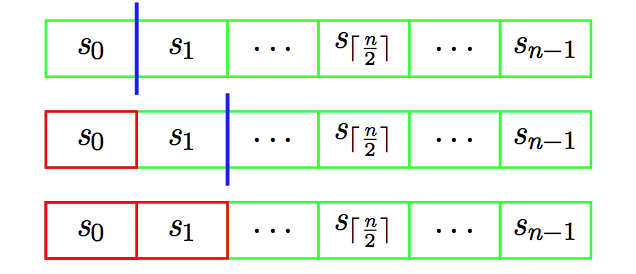
\includegraphics[width=3in]{L5-incremental-dc1.png}
%\end{figure}
%
%
% \item \textcolor{red}{\bf divide-and-conquer}: the original problem is decomposed into several independent sub-problems; thus, a feasible solution to the original problem can be constructed by assembling the solutions to independent sub-problems. 
%\begin{figure} 
%  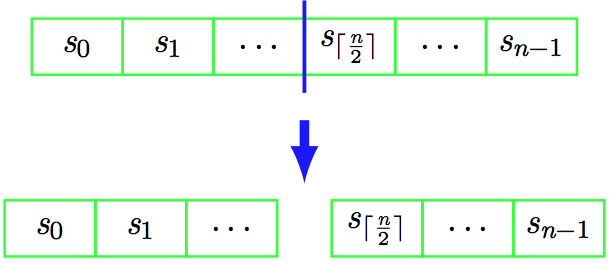
\includegraphics[width=3in]{L5-incremental-dc2.png}
%\end{figure}
%
%\end{enumerate}
%\end{itemize} 
%
%}


\frame{
\frametitle{Dynamic programming and its connection with divide-and-conquer}
\begin{itemize}
	 \item Dynamic programming typically applies to \textcolor{red}{\bf optimization problems} if: 
	 	\begin{enumerate}
			\item The original problem can be divided into smaller subproblems, and 
			\item The recursion among sub-problems has  \textcolor{red}{\bf optimal-substructure property}, i.e., the optimal solution to the original problem can be calculated through \textcolor{red}{\bf combining the optimal solutions to subproblems}. 
		\end{enumerate}
	\item Unlike the general divide-and-conquer framework, a dynamic programming algorithm usually \textcolor{red}{\bf enumerates} all possible dividing strategies. 
	\item To identify meaningful recursions, one of the key steps is to define \textcolor{red}{\bf  an appropriate general form of sub-problems}. For this aim, it is helpful to describe the solving process as \textcolor{red}{\bf a multistage decision process}.  	
	% In addition, \textcolor{red}{\bf  the repetition of computing the common subproblems} is avoided through ``programing''. 

%	 , where the original problem is a specific case of the sub-problems or can be solved using solutions to sub-problems. 
%\footnote{Here, ``programming'' means ``tabular'' rather than ``coding''. The best example of programming might be the calculation of Fibonacci numbers.  Program:   [Date: 1600-1700; Language: French;  'to write before'] } 


%\item
%Both dynamic programming and greedy techniques are \textcolor{red}{\bf  typically} applied to \textcolor{red}{\bf optimization} problems. \\
%{\it  \begin{small}
% In such problems, there can be many possible solutions. Each solution is associated with a value, and we wish to find the solution with the minimum/maximum value.
%\end{small}
%}

% \item Dynamic programming (and greedy technique) is typically used to solve an optimization problem. {\it  \begin{small}  An optimization problem usually has multiple feasible solutions, and each solution is associated with a value. The goal is to find the solution with the minimum/maximum value. \end{small} }
 %\item However, dynamic programming is not limited to optimization problems. Generally speaking, dynamic programming applies if \textcolor{red}{\bf recursion} exists, e.g. {\sc p-value calculation} problem. Sometimes the original problem should be \textcolor{red}{\bf extended} to identify meaningful \textcolor{red}{\bf recursion}. 

	\end{itemize}
}

\frame{
	\frametitle{The birth of dynamic programming}
	
	\begin{figure}
		\centering
		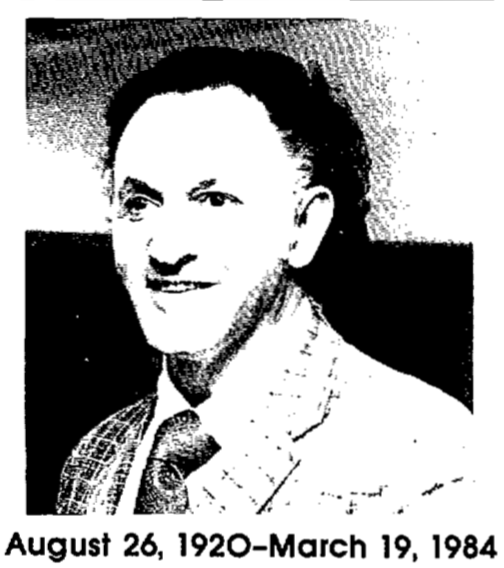
\includegraphics[width=2in]{Bellman.png}
	\end{figure}
	\begin{itemize}
		\item 		In 1952, R. Bellman proposed the dynamic programming technique when he worked at RAND corporation. The motivation is to solve multi-stage decision problems, which are difficult for the calculus of variation technique.
	\end{itemize}

}


\frame{
	\frametitle{Revisiting the {\sc Divide and Conquer} technique}
	\begin{itemize}
		\item To see whether the {\sc Divide and Conquer} technique applies on a given problem, we need to examine both \textcolor{red}{\bf  input} and \textcolor{red}{\bf output} of the problem description. 
		\begin{itemize}
			\item Examine the \textcolor{red}{\bf  input}  part to determine how to decompose the problem into subproblems of same structure but smaller size: It is relatively easy to decompose a problem into subproblems  if the input part is related to the following data structures:
			\begin{itemize}
				\item An \textcolor{red}{\bf array} with $n$ elements; 
				\item A \textcolor{red}{\bf matrix}; 
				\item A \textcolor{red}{\bf set} of $n$ elements;
				\item A \textcolor{red}{\bf tree}; 
				\item A \textcolor{red}{\bf directed acyclic graph};
				\item A \textcolor{red}{\bf general graph}.
			\end{itemize}
			\item Examine the \textcolor{red}{\bf output} part to determine how to construct the solution to the original problem using the solutions to its subproblems. 
		\end{itemize}
	\end{itemize}
}




\frame{
\begin{block}{}
 {\sc MatrixChainMultiplication} problem: recursion over \textcolor{red}{\bf sequences}
\end{block}
}

\frame{
\frametitle{{\sc MatrixChainMultiplication} problem}
\begin{block}{}
{\bf INPUT: }  \\
  A sequence of $n$ matrices $A_1, A_2, ..., A_n$; matrix $A_i$ has dimension $p_{i-1}\times p_i$;  \\
{\bf OUTPUT: } \\
 Fully parenthesizing the product $A_1 A_2 ... A_n$ in a way to minimize the number of scalar multiplications. 
\end{block}
}

\frame{
\frametitle{Let's start from a simple example} 
%\begin{figure}
% 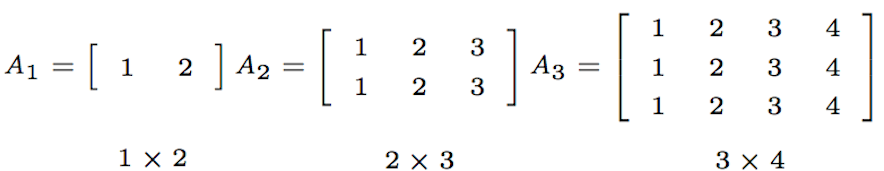
\includegraphics[width=3in] {L6-3matrices.png}
%\end{figure}

\begin{table}[!ht]
\centering
\setlength\tabcolsep{0pt} %cell margin=0
\begin{tiny}
\begin{tabular}{cccccccccccc}
 $A_1=$ & $\begin{bmatrix}
            1 & 2
        \end{bmatrix}$ & 
 $\ A_2=$ & $\begin{bmatrix}
            1 & 2 & 3\\
            1 & 2 & 3
        \end{bmatrix}$ & 
 $\ A_3=$ & $\begin{bmatrix}
            1 & 2 & 3 & 4\\
            1 & 2 & 3 & 4\\
            1 & 2 & 3 & 4
        \end{bmatrix}$ 
%        &
% $\ A_4=$ & $\begin{bmatrix}
%            1 & 2 & 3 & 4 & 5\\
%            1 & 2 & 3 & 4 & 5\\
%            1 & 2 & 3 & 4 & 5\\
%            1 & 2 & 3 & 4 & 5\\
%        \end{bmatrix}$ \\
% & $1\times 2$ & & $2\times 3$ & & $3\times 4$ &  & $4\times 5$
\end{tabular}
\end{tiny}
\end{table}


\begin{eqnarray}
\text{\tt Solutions:} &     ( (A_1) (A_2) )  (A_3 )    &   ( A_1 )  ( (A_2) (A_3) ) \nonumber \\ 
\text{\tt \#Multiplications:} &  1\times 2 \times 3  &  2  \times 3  \times 4   \nonumber \\
& +  1 \times 3 \times 4  & + 1 \times 2 \times 4 \nonumber  \\
& = 18 & = 32 \nonumber
\end{eqnarray}
\begin{itemize}
\item 
Here we assume that the calculation of $A_1 A_2$ needs $1 \times 2 \times 3$ scalar multiplications. 
\item 
The objective is to determine a calculation sequence  such that the number of multiplications is minimized. 
\end{itemize}

}



\frame{
\frametitle{The solution space size } 
\begin{itemize}
 \item Intuitively, a calculation sequence can be described as a binary tree, where each node corresponds to a subproblem.
 
 \begin{figure}
\begin{tikzpicture}[scale=1., auto,swap]
    % Draw a 7,11 network
    % First we draw the vertices
    \foreach \pos/\name in {{(0,0)/A1234}, {(-1,-1)/A12}, {(1,-1)/A34}, {(-1.5,-2)/A1}, {(-.5, -2)/A2}, {(0.5, -2)/A3}, {(1.5, -2)/A4}}
        \node[tinyvertex,draw=black, fill=blue!20] (\name) at \pos {};
    % Connect vertices with edges and draw weights
    \foreach \source/ \dest /\weight in {A1234/A12/{}, A1234/A34/{}, A12/A1/{}, A12/A2/{}, A34/A3/{}, A34/A4/{}  }
        \path[undirectededge] (\source) -- node[weight] {\small $\weight$} (\dest);
%       \draw[dashed, ->] (0,0) arc  (120:60:2);
 
   \node[above] at (0,0.2) {\tiny $ (  ( A_1 )  (A_2 ) ) ( ( A_3 ) ( A_4 ) )$};
   \node[left] at (-1.2, -1) {\tiny $ (  ( A_1 )  (A_2 ) ) $};
   \node[right] at (1.2, -1) {\tiny $ ( ( A_3 ) ( A_4 ) )$};
   \node[below] at (-1.5, -2.2) {\tiny $( A_1 )$};
   \node[below] at (-.5, -2.2) {\tiny $( A_2 )$};
   \node[below] at (.5, -2.2) {\tiny $( A_3 )$};
   \node[below] at (1.5, -2.2) {\tiny $( A_4 )$};
   
   \end{tikzpicture}
\end{figure}

%\begin{figure}
% \includegraphics[width=1.5in] {L6-matrixmultiplicationtree.eps}
%\end{figure}

 \item The total number of possible calculation sequences:  
 	\begin{center}
		${2n-2 \choose n-1 } - {2n-2 \choose n-2}$ (Catalan number) 
	\end{center}
 \item Thus, it takes exponential time to enumerate all possible calculation sequences. 
 \item Question: can we design an efficient algorithm? 
 \end{itemize}
}


\frame{
 \begin{block}{}
 A dynamic programming algorithm (by S. S. Godbole, 1973)
 \end{block} 
}

\frame{
\frametitle{Defining general form of sub-problems}
\begin{enumerate}
\item It is not easy to solve the problem directly when $n$ is large. Let's investigate whether it is possible to reduce into smaller sub-problems. 
\item Solution: a full parentheses. Let's describe the solving process as a process of \textcolor{red}{\bf multistage decisions}, where each decision is to add parentheses at a position.
\item Suppose in the optimal solution $O$, where the first \textcolor{red}{\bf decision} adds two parentheses as $\textcolor{red}{(}A_1 ... A_k\textcolor{red}{)(} A_{k+1}...A_{n}\textcolor{red}{)}$. 
%There are a total of $n-1$ options for this decision, i.e. $k=1$ or $2$, ..., or $n-1$. 
\item This decision decomposes the original problem into two \textcolor{red}{\bf independent sub-problems}: to calculate \textcolor{red}{$A_1 ... A_k$} and \textcolor{red}{$A_{k+1}...A_{n}$}. \\ 

\item Summarizing these two cases, we define the general form of sub-problems as: to calculate $A_{i}...A_{j}$ with the minimal number of scalar multiplications.
\end{enumerate}
%\begin{small} 
%{\it Here, the \textcolor{red}{\bf  independence} means that the calculation of $(A_1 ... A_k)$ does not affect the calculation of $(A_{k+1}...A_{n})$, and vice versa. } 
%\end{small}
} 

\frame{
\frametitle{Optimal substructure property}
\begin{itemize}
\item The general form of sub-problems: to calculate $A_{i}...A_{j}$ with the minimal number of scalar multiplications. Let's denote the optimal solution value to the sub-problem as $OPT(i,j)$, thus the original problem can be solved via calculating $OPT(1,n)$. 
 %\item It should be pointed out that the total number of sub-problems is polynomial ($n^2$).
%\end{itemize}
%}
%
%\frame{
%\frametitle{}
%\begin{itemize}
%\item For \textcolor{red}{\bf any solution} with the first split occurring between $A_{k}$ and $A_{k+1}$, the following equation holds:
%
%$Cost(i, j) = Cost(i, k) + Cost(k+1, j) + p_ip_{k+1}p_{j+1}$ 
%
%(Here, $Cost(i, j)$ denotes the number of multiplications needed to calculate $A_{i}...A_{j}$. The equality holds due to the independence between the two sub-problems $A_{i}...A_{k}$ and $A_{k+1}...A_{j}$.) \\ \ \\ \ \\

 \item The optimal solution to the original problem can be obtained through combining the optimal solutions to sub-problems. This recursion can be stated as the following \textcolor{red}{\bf optimal substructure property}: 
  
$OPT(1, n) = OPT(1, k) + OPT(k+1, n) + p_0p_{k}p_{n}$ 

\end{itemize}
} 

\frame{
\frametitle{Proof of the optimal substructure property}

\begin{itemize}
\item 
``Cut-and-paste'' proof: 
\begin{itemize}
\item Suppose  for  $A_1...A_k$, there is another parentheses $OPT'(1,k)$  better than $OPT(1, k)$. Then the combination of $OPT'(1,k)$ and $OPT(k+1,n)$ leads to a new solution with lower cost than $OPT(1, n)$: a contradiction. 
\item  Here, the independence between $A_1...A_k$ and $A_{k+1}...A_n$ guarantees that the substitution of $OPT(1,k)$ with $OPT'(1,k)$ does not affect solution to $A_{k+1} ... A_n$. 
\end{itemize}
\end{itemize}

}

\frame{
\frametitle{A recursive solution}
\begin{itemize}
 \item 
So far so good! The only difficulty is that we have no idea of the first splitting position $k$ in the optimal solution. \\
\item 
How to overcome this difficulty? \textcolor{red}{\bf Enumeration!} We   \textcolor{red}{\bf enumerate all possible options of the first decision}, i.e. for all $k$, $i \leq k < j$. 

\begin{figure}
\begin{tikzpicture}[scale=1., auto,swap]

    \def\d{0};
    \foreach \pos/\name in {{(0+\d,0)/root}, {(-0.5+\d,-1)/lson}, {(0.5+\d,-1)/rson}}
            \node[tinyvertex,draw=black, fill=blue!20] (\name) at \pos {};
    % Connect vertices with edges and draw weights
    \foreach \source/ \dest /\weight in {root/lson/{}, root/rson/{}}
            \path[undirectededge] (\source) -- node[weight] {\small $\weight$} (\dest);
%       \draw[dashed, ->] (0,0) arc  (120:60:2);
 
   \node[above, red, thick] at (0+\d,0.5) {\tiny $k=1$};
   \node[above] at (0+\d,0.2) {\tiny $ (  A_1 ) ( A_2 A_3 A_4 )$};
   \node[below] at (-0.5+\d, -1.1) {\tiny $( A_1 )$};
   \node[below] at (0.5+\d, -1.1) {\tiny $( A_2 A_3 A_4 )$};

   
   
   
       \def\d{2.5};
    \foreach \pos/\name in {{(0+\d,0)/root}, {(-0.5+\d,-1)/lson}, {(0.5+\d,-1)/rson}}
            \node[tinyvertex,draw=black, fill=blue!20] (\name) at \pos {};
    % Connect vertices with edges and draw weights
    \foreach \source/ \dest /\weight in {root/lson/{}, root/rson/{}}
            \path[undirectededge] (\source) -- node[weight] {\small $\weight$} (\dest);
%       \draw[dashed, ->] (0,0) arc  (120:60:2);
 
   \node[above, red, thick] at (0+\d,0.5) {\tiny $k=2$};
   \node[above] at (0+\d,0.2) {\tiny $ (  A_1  A_2 ) ( A_3 A_4 )$};
   \node[below] at (-0.5+\d, -1.1) {\tiny $( A_1 A_2 )$};
   \node[below] at (0.5+\d, -1.1) {\tiny $( A_3 A_4 )$};


    \def\d{5};
    \foreach \pos/\name in {{(0+\d,0)/root}, {(-0.5+\d,-1)/lson}, {(0.5+\d,-1)/rson}}
            \node[tinyvertex,draw=black, fill=blue!20] (\name) at \pos {};
    % Connect vertices with edges and draw weights
    \foreach \source/ \dest /\weight in {root/lson/{}, root/rson/{}}
            \path[undirectededge] (\source) -- node[weight] {\small $\weight$} (\dest);
%       \draw[dashed, ->] (0,0) arc  (120:60:2);
 
   \node[above, red, thick] at (0+\d,0.5) {\tiny $k=3$};
   \node[above] at (0+\d,0.2) {\tiny $ (  A_1 A_2 A_3 ) ( A_4 )$};
   \node[below] at (-0.5+\d, -1.1) {\tiny $( A_1 A_2 A_3  )$};
   \node[below] at (0.5+\d, -1.1) {\tiny $( A_4 )$};




   \end{tikzpicture}
\end{figure}


\item Thus we have the following recursion: 

\begin{footnotesize}
\begin{equation}
OPT(i, j) = 
\begin{cases} 0 & i=j \\
\textcolor{red}{\bf min_{i\leq k < j} } \{OPT(i, k) + OPT(k+1, j) + p_{i-1}p_{k}p_{j} \} & otherwise 
\end{cases} \nonumber 
\end{equation}
\end{footnotesize}

\end{itemize}
}

%\frame{
%\frametitle{An example of the enumeration }
%\begin{itemize}
% \item 
%Thus we have the following recursion: 
%\begin{footnotesize}
%\begin{equation}
%OPT(i, j) = 
%\begin{cases} 0 & i=j \\
%\textcolor{red}{\bf min_{i\leq k < j} } \{OPT(i, k) + OPT(k+1, j) + p_ip_{k+1}p_{j+1} \} & otherwise 
%\end{cases} \nonumber 
%\end{equation}
%\end{footnotesize}
%For example, 
%\begin{figure}
% \includegraphics[width=3.8in] {L6-matrixmultiplicationtree3.eps}
%\end{figure}
%
%%\item
%%Remember that our objective is to calculate $OPT(1, n)$. 
%\end{itemize}
%}

\frame{
	\begin{block}{}
		Implementing the recursion: trial 1
	\end{block}
} 

\frame{
\frametitle{Trial 1:  Explore the recursion in the top-down manner}
\begin{small}
{\sc RECURSIVE\_MATRIX\_CHAIN}$( i, j)$
\begin{algorithmic}[1]
\IF {$i == j$ }
	\STATE return $0$;
\ENDIF
\STATE $OPT(i, j) = +\infty;$
\FOR{$k=i$ to $j-1$} 
	\STATE $q = $ {\sc RECURSIVE\_MATRIX\_CHAIN}$(i, k)$ 
	\STATE $\quad  + $ {\sc RECURSIVE\_MATRIX\_CHAIN}$(k+1, j)$
	\STATE $\quad  + p_{i-1}p_{k}p_{j};$
	\IF {$q < OPT(i, j) $} 
		\STATE $OPT(i, j) = q;$
	\ENDIF 
\ENDFOR
\RETURN{$OPT(i, j);$}
\end{algorithmic}
\end{small}

\begin{itemize}
\item 
Note: The optimal solution to the original problem  can be obtained through calling {\sc RECURSIVE\_MATRIX\_CHAIN}$(1, n)$.
\end{itemize}

}

\frame{
\frametitle{An example} 

%	\begin{figure}
%		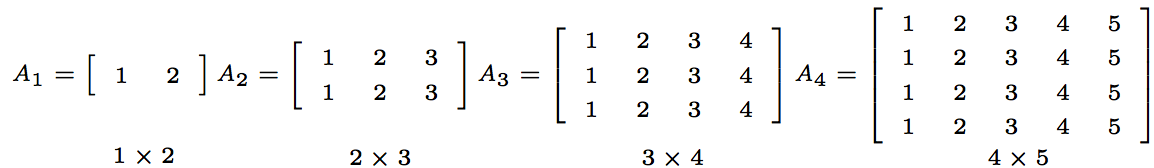
\includegraphics[width=4in]{Problems/L6-4matrices.png}
%	\end{figure}

\begin{table}[!ht]
\centering
\setlength\tabcolsep{0pt} %cell margin=0
\begin{tiny}
\begin{tabular}{cccccccccccc}
 $A_1=$ & $\begin{bmatrix}
            1 & 2
        \end{bmatrix}$ & 
 $\ A_2=$ & $\begin{bmatrix}
            1 & 2 & 3\\
            1 & 2 & 3
        \end{bmatrix}$ & 
 $\ A_3=$ & $\begin{bmatrix}
            1 & 2 & 3 & 4\\
            1 & 2 & 3 & 4\\
            1 & 2 & 3 & 4
        \end{bmatrix}$ &
 $\ A_4=$ & $\begin{bmatrix}
            1 & 2 & 3 & 4 & 5\\
            1 & 2 & 3 & 4 & 5\\
            1 & 2 & 3 & 4 & 5\\
            1 & 2 & 3 & 4 & 5\\
        \end{bmatrix}$ \\
 & $1\times 2$ & & $2\times 3$ & & $3\times 4$ &  & $4\times 5$
\end{tabular}
\end{tiny}
\end{table}


\begin{figure}
\begin{tikzpicture}[scale=0.8, auto,swap]
    % Draw a 7,11 network
    % First we draw the vertices
     \draw[thick] (0,0)  -- (4.5, -1);
     \draw[thick]  (0,0) --  (-4.5, -1);

     \draw[thick] (0,0)  -- (6.5, -1);
     \draw[thick]  (0,0) --  (-6.5, -1);
       \node[tinyvertex,draw=black, fill=blue!20] (A4) at (6.5, -1) {};
        \node[tinyvertex,draw=black, fill=blue!20] (A1) at (-6.5, -1) {};
   \node[left] at (A1.west) {\tiny $A_1$};
    \node[right] at (A4.east) {\tiny $A_{4}$};

 
    \def\dx{0};
    \def\dy{0}
    \foreach \pos/\name in {{(0+\dx,0+\dy)/R1}, {(-1+\dx,-1+\dy)/L}, {(1+\dx,-1+\dy)/R}, {(-1.5+\dx,-2+\dy)/LL}, {(-.5+\dx, -2+\dy)/LR}, {(0.5+\dx, -2+\dy)/RL}, {(1.5+\dx, -2+\dy)/RR}}
        \node[tinyvertex,draw=black, fill=blue!20] (\name) at \pos {};
    % Connect vertices with edges and draw weights
    \foreach \source/ \dest /\weight in {R1/L/{}, R1/R/{}, L/LL/{}, L/LR/{}, R/RL/{}, R/RR/{}  }
        \path[undirectededge] (\source) -- node[weight] {\small $\weight$} (\dest);
%       \draw[dashed, ->] (0,0) arc  (120:60:2);
    \node[above] at (R1.north) {\tiny $A_1A_2A_3A_4$};
   \node[left] at (L.west) {\tiny $A_1A_2$};
   \node[right] at (R.east) {\tiny $A_3A_4$};
   \node[below] at (LL.south) {\tiny $A_1$};
   \node[below] at (LR.south) {\tiny $A_2$};   
   \node[below] at (RL.south) {\tiny $A_3$};
    \node[below] at (RR.south) {\tiny $A_4$};


   
   
   %right sub-tree
      \draw[thick] (4.5,-1)  -- (2.5, -2);
      \draw[thick] (4.5,-1)  -- (6.5, -2);
       \node[tinyvertex,draw=black, fill=blue!20] (A1) at (2.5,-2) {};
        \node[tinyvertex,draw=black, fill=blue!20] (A3) at (6.5, -2) {};
  \node[below] at (A1.south) {\tiny $A_1$};
  \node[below] at (A3.south) {\tiny $A_3$};
 
    \def\dx{4.5};
    \def\dy{-1}
    \foreach \pos/\name in {{(0+\dx,0+\dy)/R1}, {(-1+\dx,-1+\dy)/L}, {(1+\dx,-1+\dy)/R}, {(-1.5+\dx,-2+\dy)/LL}, {(-.5+\dx, -2+\dy)/LR}, {(0.5+\dx, -2+\dy)/RL}, {(1.5+\dx, -2+\dy)/RR}}
        \node[tinyvertex,draw=black, fill=blue!20] (\name) at \pos {};
    % Connect vertices with edges and draw weights
    \foreach \source/ \dest /\weight in {R1/L/{}, R1/R/{}, L/LL/{}, L/LR/{}, R/RL/{}, R/RR/{}  }
        \path[undirectededge] (\source) -- node[weight] {\small $\weight$} (\dest);
%       \draw[dashed, ->] (0,0) arc  (120:60:2);

    \node[left] at (R1.west) {\tiny $A_{1}A_2A_{3}$};   
    \node[right] at (L) {\tiny $A_2A_{3}$};   
    \node[left] at (R) {\tiny $A_1A_{2}$};   
    \node[below] at (LL.south) {\tiny $A_2$};   
    \node[below] at (LR.south) {\tiny $A_3$};   
   \node[below] at (RL.south) {\tiny $A_1$};   
   \node[below] at (RR.south) {\tiny $A_2$};   




%left sub-tree
 
       \draw[thick] (-4.5,-1)  -- (-2.5, -2);
      \draw[thick] (-4.5,-1)  -- (-6.5, -2);
       \node[tinyvertex,draw=black, fill=blue!20] (A2) at (-2.5,-2) {};
        \node[tinyvertex,draw=black, fill=blue!20] (A4) at (-6.5, -2) {};
  \node[below] at (A2.south) {\tiny $A_4$};
  \node[below] at (A4.south) {\tiny $A_2$};

      
    \def\dx{-4.5};
    \def\dy{-1}
    \foreach \pos/\name in {{(0+\dx,0+\dy)/R1}, {(-1+\dx,-1+\dy)/L}, {(1+\dx,-1+\dy)/R}, {(-1.5+\dx,-2+\dy)/LL}, {(-.5+\dx, -2+\dy)/LR}, {(0.5+\dx, -2+\dy)/RL}, {(1.5+\dx, -2+\dy)/RR}}
        \node[tinyvertex,draw=black, fill=blue!20] (\name) at \pos {};
    % Connect vertices with edges and draw weights
    \foreach \source/ \dest /\weight in {R1/L/{}, R1/R/{}, L/LL/{}, L/LR/{}, R/RL/{}, R/RR/{}  }
        \path[undirectededge] (\source) -- node[weight] {\small $\weight$} (\dest);
%       \draw[dashed, ->] (0,0) arc  (120:60:2);
      \node[right] at (R1.east) {\tiny $A_2A_{3}A_{4}$};
    \node[right] at (L) {\tiny $A_3A_{4}$};   
    \node[left] at (R) {\tiny $A_2A_{3}$};   
    \node[below] at (LL.south) {\tiny $A_3$};   
    \node[below] at (LR.south) {\tiny $A_4$};   
   \node[below] at (RL.south) {\tiny $A_2$};   
   \node[below] at (RR.south) {\tiny $A_3$};   

 
 
   
   \end{tikzpicture}
\end{figure}
%
%\begin{figure}
%\begin{center}
% \includegraphics[width=4.2in] {L6-matrixmultiplicationalgo1tree.eps}
%\end{center}
%\end{figure}
\begin{itemize}
	\item Note: each node of the recursion tree represents a subproblem. 
\end{itemize}

}

\frame{
\frametitle{However, this is not a good implementation }
\begin{theorem}
Algorithm {\sc RECURSIVE-MATRIX-CHAIN} costs exponential time. 
\end{theorem}
\begin{itemize}
	\item Let $T(n)$ denote the time used to calculate product of $n$ matrices. 
Then $T(n) \geq 1 + \sum_{k=1}^{n-1} ( T(k) + T(n-k) + 1 )$ for $n>1$.
\end{itemize}

\begin{figure}
\begin{tikzpicture}[scale=0.8, auto,swap]
    % Draw a 7,11 network
    % First we draw the vertices
    
    \draw[ultra thick, red ] (-7.25, -1.3) rectangle (7.25, 1.1);
    
        \node[above, thick, red] at (0, 0.5) {\tiny $T(4)$};

    
     \draw[thick] (0,0)  -- (4.5, -1);
     \draw[thick]  (0,0) --  (-4.5, -1);

     \draw[thick] (0,0)  -- (6.5, -1);
     \draw[thick]  (0,0) --  (-6.5, -1);
       \node[tinyvertex,draw=black, fill=blue!20] (A4) at (6.5, -1) {};
        \node[tinyvertex,draw=black, fill=blue!20] (A1) at (-6.5, -1) {};
   \node[left] at (A1.west) {\tiny $A_1$};
    \node[right] at (A4.east) {\tiny $A_{4}$};

         \node[above, thick, red] at (A1.north) {\tiny $T(1)$};
         \node[above, thick, red] at (A4.north) {\tiny $T(1)$};
 
    \def\dx{0};
    \def\dy{0}
    \foreach \pos/\name in {{(0+\dx,0+\dy)/R1}, {(-1+\dx,-1+\dy)/L}, {(1+\dx,-1+\dy)/R}, {(-1.5+\dx,-2+\dy)/LL}, {(-.5+\dx, -2+\dy)/LR}, {(0.5+\dx, -2+\dy)/RL}, {(1.5+\dx, -2+\dy)/RR}}
        \node[tinyvertex,draw=black, fill=blue!20] (\name) at \pos {};
    % Connect vertices with edges and draw weights
    \foreach \source/ \dest /\weight in {R1/L/{}, R1/R/{}, L/LL/{}, L/LR/{}, R/RL/{}, R/RR/{}  }
        \path[undirectededge] (\source) -- node[weight] {\small $\weight$} (\dest);
%       \draw[dashed, ->] (0,0) arc  (120:60:2);
    \node[above] at (R1.north) {\tiny $A_1A_2A_3A_4$};
   \node[left] at (L.west) {\tiny $A_1A_2$};
   \node[right] at (R.east) {\tiny $A_3A_4$};
   \node[below] at (LL.south) {\tiny $A_1$};
   \node[below] at (LR.south) {\tiny $A_2$};   
   \node[below] at (RL.south) {\tiny $A_3$};
    \node[below] at (RR.south) {\tiny $A_4$};

         \node[above, thick, red] at (L.north) {\tiny $T(2)$};
         \node[above, thick, red] at (R.north) {\tiny $T(2)$};
   
   
   %right sub-tree
      \draw[thick] (4.5,-1)  -- (2.5, -2);
      \draw[thick] (4.5,-1)  -- (6.5, -2);
       \node[tinyvertex,draw=black, fill=blue!20] (A1) at (2.5,-2) {};
        \node[tinyvertex,draw=black, fill=blue!20] (A3) at (6.5, -2) {};
  \node[below] at (A1.south) {\tiny $A_1$};
  \node[below] at (A3.south) {\tiny $A_3$};
 
    \def\dx{4.5};
    \def\dy{-1}
    \foreach \pos/\name in {{(0+\dx,0+\dy)/R1}, {(-1+\dx,-1+\dy)/L}, {(1+\dx,-1+\dy)/R}, {(-1.5+\dx,-2+\dy)/LL}, {(-.5+\dx, -2+\dy)/LR}, {(0.5+\dx, -2+\dy)/RL}, {(1.5+\dx, -2+\dy)/RR}}
        \node[tinyvertex,draw=black, fill=blue!20] (\name) at \pos {};
    % Connect vertices with edges and draw weights
    \foreach \source/ \dest /\weight in {R1/L/{}, R1/R/{}, L/LL/{}, L/LR/{}, R/RL/{}, R/RR/{}  }
        \path[undirectededge] (\source) -- node[weight] {\small $\weight$} (\dest);
%       \draw[dashed, ->] (0,0) arc  (120:60:2);

    \node[left] at (R1.west) {\tiny $A_{1}A_2A_{3}$};   
    \node[right] at (L) {\tiny $A_2A_{3}$};   
    \node[left] at (R) {\tiny $A_1A_{2}$};   
    \node[below] at (LL.south) {\tiny $A_2$};   
    \node[below] at (LR.south) {\tiny $A_3$};   
   \node[below] at (RL.south) {\tiny $A_1$};   
   \node[below] at (RR.south) {\tiny $A_2$};   

         \node[above, thick, red] at (R1.north) {\tiny $T(3)$};



%left sub-tree
 
       \draw[thick] (-4.5,-1)  -- (-2.5, -2);
      \draw[thick] (-4.5,-1)  -- (-6.5, -2);
       \node[tinyvertex,draw=black, fill=blue!20] (A2) at (-2.5,-2) {};
        \node[tinyvertex,draw=black, fill=blue!20] (A4) at (-6.5, -2) {};
  \node[below] at (A2.south) {\tiny $A_4$};
  \node[below] at (A4.south) {\tiny $A_2$};

      
    \def\dx{-4.5};
    \def\dy{-1}
    \foreach \pos/\name in {{(0+\dx,0+\dy)/R1}, {(-1+\dx,-1+\dy)/L}, {(1+\dx,-1+\dy)/R}, {(-1.5+\dx,-2+\dy)/LL}, {(-.5+\dx, -2+\dy)/LR}, {(0.5+\dx, -2+\dy)/RL}, {(1.5+\dx, -2+\dy)/RR}}
        \node[tinyvertex,draw=black, fill=blue!20] (\name) at \pos {};
    % Connect vertices with edges and draw weights
    \foreach \source/ \dest /\weight in {R1/L/{}, R1/R/{}, L/LL/{}, L/LR/{}, R/RL/{}, R/RR/{}  }
        \path[undirectededge] (\source) -- node[weight] {\small $\weight$} (\dest);
%       \draw[dashed, ->] (0,0) arc  (120:60:2);
      \node[right] at (R1.east) {\tiny $A_2A_{3}A_{4}$};
    \node[right] at (L) {\tiny $A_3A_{4}$};   
    \node[left] at (R) {\tiny $A_2A_{3}$};   
    \node[below] at (LL.south) {\tiny $A_3$};   
    \node[below] at (LR.south) {\tiny $A_4$};   
   \node[below] at (RL.south) {\tiny $A_2$};   
   \node[below] at (RR.south) {\tiny $A_3$};   

 
          \node[above, thick, red] at (R1.north) {\tiny $T(3)$};
 
   
   \end{tikzpicture}
\end{figure}


%\begin{figure}
%\begin{center}
% \includegraphics[width=4in] {L6-matrixmultiplicationalgo1analysis.eps}
%\end{center}
%\end{figure}
}

\frame{
%\frametitle{Time-complexity analysis}
%\begin{theorem}
%Algorithm {\sc RECURSIVE-MATRIX-CHAIN} costs exponential time. 
%\end{theorem}
\begin{proof} 
\begin{itemize}
	\item We shall prove $T(n) \geq 2^{n-1}$ using the substitution technique. \\
	\begin{itemize}
		\item  Basis: $T(1) \geq 1 = 2^{1-1}$. 
		\item Induction: 
\begin{eqnarray}
T(n) & \geq &  1 + \sum\nolimits_{k=1}^{n-1} ( T(k) + T(n-k) + 1 ) \\
     & = & n + 2 \sum\nolimits_{k=1}^{n-1} T(k) \\
     & \geq & n + 2 \sum\nolimits_{k=1}^{n-1} 2^{k-1} \\
     & \geq & n + 2 ( 2^{n-1} - 1 ) \\
     & \geq & n + 2^n - 2 \\
     & \geq & 2^{n-1}
\end{eqnarray}
	\end{itemize}
\end{itemize}
\end{proof}
}



\frame{
\frametitle{Why the first trial failed? }
%\begin{figure}
% \includegraphics[width=4.2in] {L6-matrixmultiplicationalgo1repeat.eps}
%\end{figure}


\begin{figure}
\begin{tikzpicture}[scale=0.8, auto,swap]
    % Draw a 7,11 network
    % First we draw the vertices
    
   
     \draw[thick] (0,0)  -- (4.5, -1);
     \draw[thick]  (0,0) --  (-4.5, -1);

     \draw[thick] (0,0)  -- (6.5, -1);
     \draw[thick]  (0,0) --  (-6.5, -1);
       \node[tinyvertex,draw=black, fill=red] (A4) at (6.5, -1) {};
        \node[tinyvertex,draw=black, fill=blue!20] (A1) at (-6.5, -1) {};
   \node[left] at (A1.west) {\tiny $A_1$};
    \node[right] at (A4.east) {\tiny $A_{4}$};


%middle tree
    \def\dx{0};
    \def\dy{0}
    \foreach \pos/\name in {{(0+\dx,0+\dy)/R1}, {(-1+\dx,-1+\dy)/L}, {(1+\dx,-1+\dy)/R}, {(-1.5+\dx,-2+\dy)/LL}, {(-.5+\dx, -2+\dy)/LR}, {(0.5+\dx, -2+\dy)/RL}, {(1.5+\dx, -2+\dy)/RR}}
        \node[tinyvertex,draw=black, fill=blue!20] (\name) at \pos {};
    % Connect vertices with edges and draw weights
    \foreach \source/ \dest /\weight in {R1/L/{}, R1/R/{}, L/LL/{}, L/LR/{}, R/RL/{}, R/RR/{}  }
        \path[undirectededge] (\source) -- node[weight] {\small $\weight$} (\dest);
%       \draw[dashed, ->] (0,0) arc  (120:60:2);
    \node[above] at (R1.north) {\tiny $A_1A_2A_3A_4$};
   \node[left] at (L.west) {\tiny $A_1A_2$};
   \node[right] at (R.east) {\tiny $A_3A_4$};
   \node[below] at (LL.south) {\tiny $A_1$};
   \node[below] at (LR.south) {\tiny $A_2$};   
   \node[below] at (RL.south) {\tiny $A_3$};
    \node[below] at (RR.south) {\tiny $A_4$};

        \node[tinyvertex,draw=black, fill=red]  at  (R) {};
        \node[tinyvertex,draw=black, fill=red]  at  (LR) {};        
         \node[tinyvertex,draw=black, fill=red]  at  (RR) {};
                 \node[tinyvertex,draw=black, fill=red]  at  (RL) {};
                 
                 
                   
   %right sub-tree
      \draw[thick] (4.5,-1)  -- (2.5, -2);
      \draw[thick] (4.5,-1)  -- (6.5, -2);
       \node[tinyvertex,draw=black, fill=red] (A1) at (2.5,-2) {};
        \node[tinyvertex,draw=black, fill=red] (A3) at (6.5, -2) {};
  \node[below] at (A1.south) {\tiny $A_1$};
  \node[below] at (A3.south) {\tiny $A_3$};
 
    \def\dx{4.5};
    \def\dy{-1}
    \foreach \pos/\name in {{(0+\dx,0+\dy)/R1}, {(-1+\dx,-1+\dy)/L}, {(1+\dx,-1+\dy)/R}, {(-1.5+\dx,-2+\dy)/LL}, {(-.5+\dx, -2+\dy)/LR}, {(0.5+\dx, -2+\dy)/RL}, {(1.5+\dx, -2+\dy)/RR}}
        \node[tinyvertex,draw=black, fill=blue!20] (\name) at \pos {};
    % Connect vertices with edges and draw weights
    \foreach \source/ \dest /\weight in {R1/L/{}, R1/R/{}, L/LL/{}, L/LR/{}, R/RL/{}, R/RR/{}  }
        \path[undirectededge] (\source) -- node[weight] {\small $\weight$} (\dest);
%       \draw[dashed, ->] (0,0) arc  (120:60:2);

    \node[left] at (R1.west) {\tiny $A_{1}A_2A_{3}$};   
    \node[right] at (L) {\tiny $A_2A_{3}$};   
    \node[left] at (R) {\tiny $A_1A_{2}$};   
    \node[below] at (LL.south) {\tiny $A_2$};   
    \node[below] at (LR.south) {\tiny $A_3$};   
   \node[below] at (RL.south) {\tiny $A_1$};   
   \node[below] at (RR.south) {\tiny $A_2$};   

        \node[tinyvertex,draw=black, fill=red]  at  (L) {};
        \node[tinyvertex,draw=black, fill=red]  at  (R) {};
        \node[tinyvertex,draw=black, fill=red]  at  (LR) {};
        \node[tinyvertex,draw=black, fill=red]  at  (RR) {};
        \node[tinyvertex,draw=black, fill=red]  at  (RL) {};
        \node[tinyvertex,draw=black, fill=red]  at  (LL) {};
 



%left sub-tree
 
       \draw[thick] (-4.5,-1)  -- (-2.5, -2);
      \draw[thick] (-4.5,-1)  -- (-6.5, -2);
       \node[tinyvertex,draw=black, fill=red] (A4) at (-2.5,-2) {};
        \node[tinyvertex,draw=black, fill=blue!20] (A2) at (-6.5, -2) {};
  \node[below] at (A4.south) {\tiny $A_4$};
  \node[below] at (A2.south) {\tiny $A_2$};

      
    \def\dx{-4.5};
    \def\dy{-1}
    \foreach \pos/\name in {{(0+\dx,0+\dy)/R1}, {(-1+\dx,-1+\dy)/L}, {(1+\dx,-1+\dy)/R}, {(-1.5+\dx,-2+\dy)/LL}, {(-.5+\dx, -2+\dy)/LR}, {(0.5+\dx, -2+\dy)/RL}, {(1.5+\dx, -2+\dy)/RR}}
        \node[tinyvertex,draw=black, fill=blue!20] (\name) at \pos {};
    % Connect vertices with edges and draw weights
    \foreach \source/ \dest /\weight in {R1/L/{}, R1/R/{}, L/LL/{}, L/LR/{}, R/RL/{}, R/RR/{}  }
        \path[undirectededge] (\source) -- node[weight] {\small $\weight$} (\dest);
%       \draw[dashed, ->] (0,0) arc  (120:60:2);
      \node[right] at (R1.east) {\tiny $A_2A_{3}A_{4}$};
    \node[right] at (L) {\tiny $A_3A_{4}$};   
    \node[left] at (R) {\tiny $A_2A_{3}$};   
    \node[below] at (LL.south) {\tiny $A_3$};   
    \node[below] at (LR.south) {\tiny $A_4$};   
   \node[below] at (RL.south) {\tiny $A_2$};   
   \node[below] at (RR.south) {\tiny $A_3$};   

        \node[tinyvertex,draw=black, fill=red]  at  (RL) {};
         \node[tinyvertex,draw=black, fill=red]  at  (RR) {};

   \end{tikzpicture}
\end{figure}

\begin{itemize}
 \item 
Reason: There are only $O(n^2)$ subproblems. However, some subproblems (in red) were solved repeatedly.
\item 
Solution: \textcolor{red}{\bf memorize the solutions to subproblems} using an array $OPT[1..n; 1..n]$ for further look-up. The calculation of Fibonacci number is a good example of the power of the ``memorizing" technique. 

\end{itemize}
}

\frame{
	\begin{block}{}
		Implementing the recursion: trial 2
	\end{block}
} 

\frame{
\frametitle{The ``memorizing"  technique  }
\begin{small}
{\sc MEMORIZE\_MATRIX\_CHAIN}$(i,j)$
\begin{algorithmic}[1]
\IF{\textcolor{red}{$OPT[i, j] \neq NULL $ } }
\RETURN{\textcolor{red}{$OPT(i, j)$; } }
\ENDIF
\IF {$ i == j $ }
\STATE $OPT[ i, j] = 0;$
\ELSE 
\FOR{$k= i$ to $j-1$} 
\STATE $q = $   {\sc MEMORIZE\_MATRIX\_CHAIN}$(i, k)$ 
\STATE $\qquad  + ${\sc MEMORIZE\_MATRIX\_CHAIN}$( k+1, j)$
\STATE $\qquad  + p_{i-1}p_{k}p_{j};$
\IF {$q < OPT[i, j] $} 
\STATE $OPT[i, j] = q;$
\ENDIF 
\ENDFOR
\ENDIF
\RETURN{$OPT[i, j];$ }
\end{algorithmic}
\end{small}

}

\frame{
\frametitle{The ``memorizing"  technique cont'd  }

\begin{itemize}
\item  The original problem can be solved by calling {\sc MEMORIZE\_MATRIX\_CHAIN}$( 1, n)$ with all $OPT[i,j]$  initialized as {\sc NULL}. 
 \item Time complexity: $O(n^3)$ (The calculation of each entry $OPT[i, j]$ makes $O(n)$ recursive calls in line $8$.) 
 \item Note that there are exponential ways of fully parenthesizing. The DP  algorithm find the optimal solution in  only $O(n^3)$ time since it avoids enumerating some redundant  fully parenthesizing. 
 \end{itemize}
}


\frame{
	\begin{block}{}
		Implementing the recursion faster: trial 3
	\end{block}
} 

\frame{
\frametitle{Trial 3: Faster implementation: unrolling the recursion in the bottom-up manner}

\begin{small}
{\sc MATRIX\_CHAIN\_MULTIPLICATION}$(p_0, p_1, ..., p_{n})$
\begin{algorithmic}[1]
\FOR{$i=1$ to $n$ }
\STATE $OPT(i,i)=0;$
\ENDFOR 
\FOR{$l=2$ to $n$ }
  \FOR{$i=1$ to $n-l+1$ }
    \STATE $j=i+l-1;$
    \STATE $OPT(i,j)=+\infty$;
    \FOR{$k= i$ to $j-1$} 
      \STATE $q = OPT(i,k) + OPT(k+1,j) +  p_{i-1}p_{k}p_{j};$
      \IF {$q < OPT(i, j) $} 
	\STATE $OPT(i, j) = q;$
	\STATE $S(i,j) = k;$
      \ENDIF 
    \ENDFOR
  \ENDFOR
\ENDFOR
\RETURN{$OPT(1,n)$;}
\end{algorithmic}
\end{small}
}

\frame{
\frametitle{Recursion tree: an intuitive view of the bottom-up calculation}

%\begin{figure}
% \includegraphics[width=4.2in] {L6-matrixmultiplicationalgo2tree.eps}
%\end{figure}

\begin{figure}
\begin{tikzpicture}[scale=0.8, auto,swap]
    % Draw a 7,11 network
    % First we draw the vertices
    
   
     \draw[thick] (0,0)  -- (4.5, -1);
     \draw[thick]  (0,0) --  (-4.5, -1);

     \draw[thick] (0,0)  -- (6.5, -1);
     \draw[thick]  (0,0) --  (-6.5, -1);
       \node[tinyvertex,draw=black, fill=red] (A4) at (6.5, -1) {};
        \node[tinyvertex,draw=black, fill=red] (A1) at (-6.5, -1) {};
   \node[left] at (A1.west) {\tiny $A_1$};
    \node[right] at (A4.east) {\tiny $A_{4}$};


%middle tree
    \def\dx{0};
    \def\dy{0}
    \foreach \pos/\name in {{(0+\dx,0+\dy)/R1}, {(-1+\dx,-1+\dy)/L}, {(1+\dx,-1+\dy)/R}, {(-1.5+\dx,-2+\dy)/LL}, {(-.5+\dx, -2+\dy)/LR}, {(0.5+\dx, -2+\dy)/RL}, {(1.5+\dx, -2+\dy)/RR}}
        \node[tinyvertex,draw=black, fill=blue!20] (\name) at \pos {};
    % Connect vertices with edges and draw weights
    \foreach \source/ \dest /\weight in {R1/L/{}, R1/R/{}, L/LL/{}, L/LR/{}, R/RL/{}, R/RR/{}  }
        \path[undirectededge] (\source) -- node[weight] {\small $\weight$} (\dest);
%       \draw[dashed, ->] (0,0) arc  (120:60:2);
    \node[above] at (R1.north) {\tiny $A_1A_2A_3A_4$};
   \node[left] at (L.west) {\tiny $A_1A_2$};
   \node[right] at (R.east) {\tiny $A_3A_4$};
   \node[below] at (LL.south) {\tiny $A_1$};
   \node[below] at (LR.south) {\tiny $A_2$};   
   \node[below] at (RL.south) {\tiny $A_3$};
    \node[below] at (RR.south) {\tiny $A_4$};

  \node[tinyvertex,draw=black, fill=blue]  at  (R1) {};
  \node[tinyvertex,draw=black, fill=green]  at  (L) {};
  \node[tinyvertex,draw=black, fill=green]  at  (R) {};
        \node[tinyvertex,draw=black, fill=red]  at  (LL) {};
        \node[tinyvertex,draw=black, fill=red]  at  (LR) {};        
         \node[tinyvertex,draw=black, fill=red]  at  (RR) {};
                 \node[tinyvertex,draw=black, fill=red]  at  (RL) {};
                 
                 
                   
   %right sub-tree
      \draw[thick] (4.5,-1)  -- (2.5, -2);
      \draw[thick] (4.5,-1)  -- (6.5, -2);
       \node[tinyvertex,draw=black, fill=red] (A1) at (2.5,-2) {};
        \node[tinyvertex,draw=black, fill=red] (A3) at (6.5, -2) {};
  \node[below] at (A1.south) {\tiny $A_1$};
  \node[below] at (A3.south) {\tiny $A_3$};
 
    \def\dx{4.5};
    \def\dy{-1}
    \foreach \pos/\name in {{(0+\dx,0+\dy)/R1}, {(-1+\dx,-1+\dy)/L}, {(1+\dx,-1+\dy)/R}, {(-1.5+\dx,-2+\dy)/LL}, {(-.5+\dx, -2+\dy)/LR}, {(0.5+\dx, -2+\dy)/RL}, {(1.5+\dx, -2+\dy)/RR}}
        \node[tinyvertex,draw=black, fill=blue!20] (\name) at \pos {};
    % Connect vertices with edges and draw weights
    \foreach \source/ \dest /\weight in {R1/L/{}, R1/R/{}, L/LL/{}, L/LR/{}, R/RL/{}, R/RR/{}  }
        \path[undirectededge] (\source) -- node[weight] {\small $\weight$} (\dest);
%       \draw[dashed, ->] (0,0) arc  (120:60:2);

    \node[left] at (R1.west) {\tiny $A_{1}A_2A_{3}$};   
    \node[right] at (L) {\tiny $A_2A_{3}$};   
    \node[left] at (R) {\tiny $A_1A_{2}$};   
    \node[below] at (LL.south) {\tiny $A_2$};   
    \node[below] at (LR.south) {\tiny $A_3$};   
   \node[below] at (RL.south) {\tiny $A_1$};   
   \node[below] at (RR.south) {\tiny $A_2$};   

        \node[tinyvertex,draw=black, fill=orange]  at  (R1) {};
        \node[tinyvertex,draw=black, fill=green]  at  (L) {};
        \node[tinyvertex,draw=black, fill=green]  at  (R) {};
        \node[tinyvertex,draw=black, fill=red]  at  (LR) {};
        \node[tinyvertex,draw=black, fill=red]  at  (RR) {};
        \node[tinyvertex,draw=black, fill=red]  at  (RL) {};
        \node[tinyvertex,draw=black, fill=red]  at  (LL) {};
 



%left sub-tree
 
       \draw[thick] (-4.5,-1)  -- (-2.5, -2);
      \draw[thick] (-4.5,-1)  -- (-6.5, -2);
       \node[tinyvertex,draw=black, fill=red] (A4) at (-2.5,-2) {};
        \node[tinyvertex,draw=black, fill=red] (A2) at (-6.5, -2) {};
  \node[below] at (A4.south) {\tiny $A_4$};
  \node[below] at (A2.south) {\tiny $A_2$};

      
    \def\dx{-4.5};
    \def\dy{-1}
    \foreach \pos/\name in {{(0+\dx,0+\dy)/R1}, {(-1+\dx,-1+\dy)/L}, {(1+\dx,-1+\dy)/R}, {(-1.5+\dx,-2+\dy)/LL}, {(-.5+\dx, -2+\dy)/LR}, {(0.5+\dx, -2+\dy)/RL}, {(1.5+\dx, -2+\dy)/RR}}
        \node[tinyvertex,draw=black, fill=blue!20] (\name) at \pos {};
    % Connect vertices with edges and draw weights
    \foreach \source/ \dest /\weight in {R1/L/{}, R1/R/{}, L/LL/{}, L/LR/{}, R/RL/{}, R/RR/{}  }
        \path[undirectededge] (\source) -- node[weight] {\small $\weight$} (\dest);
%       \draw[dashed, ->] (0,0) arc  (120:60:2);
      \node[right] at (R1.east) {\tiny $A_2A_{3}A_{4}$};
    \node[right] at (L) {\tiny $A_3A_{4}$};   
    \node[left] at (R) {\tiny $A_2A_{3}$};   
    \node[below] at (LL.south) {\tiny $A_3$};   
    \node[below] at (LR.south) {\tiny $A_4$};   
   \node[below] at (RL.south) {\tiny $A_2$};   
   \node[below] at (RR.south) {\tiny $A_3$};   


        \node[tinyvertex,draw=black, fill=orange]  at  (R1) {};
        \node[tinyvertex,draw=black, fill=green]  at  (L) {};
        \node[tinyvertex,draw=black, fill=green]  at  (R) {};
        \node[tinyvertex,draw=black, fill=red]  at  (LR) {};
        \node[tinyvertex,draw=black, fill=red]  at  (RR) {};
        \node[tinyvertex,draw=black, fill=red]  at  (RL) {};
        \node[tinyvertex,draw=black, fill=red]  at  (LL) {};
 
         
         
   \end{tikzpicture}
\end{figure}

\begin{itemize}
 	\item Solving sub-problems in a bottom-up manner, i.e.  
	\begin{enumerate}
 		\item Solving the sub-problems in red first;
 		\item Then solving the sub-problems in green;
 		\item Then solving the sub-problems in orange;
 		\item Finally we can solve the original problem in blue.
	\end{enumerate}
\end{itemize}
}

\frame{
\frametitle{Step 1 of the bottom-up algorithm}

	\begin{figure}
    
\begin{tikzpicture}[scale=0.9, auto,swap]
  
  	\def\d{0.7};
	
	%draw index 
 \def\dy{1};
 \def\dx{0};
 \node at ( 2 * \d + \dx * \d, \dy * \d +  \d ) {\tt OPT };

    \foreach \i/\num/\name in {1/1/s1,2/2/s2,3/3/s3,4/4/s4 }{
           \node (\name) at (\i*\d+\d/2 + \dx*\d - \d, \d/2 + \dy * \d) {\tiny $\num$};
    }

 \def\dy{0};
 \def\dx{0};
    \foreach \i/\num/\name in {1/1/s1,2/2/s2,3/3/s3,4/4/s4 }{
         \node (\name) at ( 4*\d+\d/2  + \dx * \d,  0.0 - \i*\d + \d/2 - \dy * \d + \d){\tiny $\num$};
    }

    
	
 \def\dy{0};
 \def\dx{0};
    \foreach \i/\num/\name in {0/0/s8,1/6/s7,2//s6,3//s5 }{
             \draw[  thick ] (\i*\d + \dx*\d,  0+ \dy*\d) rectangle (\i*\d+\d + \dx*\d, \d + \dy*\d);
         \node (\name) at (\i*\d+\d/2 + \dx*\d, \d/2 + \dy*\d) {\tiny $\num$};
    }
 \def\dy{-1};
 \def\dx{1};
    \foreach \i/\num/\name in {0/0/s8,1/24/s7,2//s6}{
             \draw[  thick ] (\i*\d + \dx*\d,  0+ \dy*\d) rectangle (\i*\d+\d + \dx*\d, \d + \dy*\d);
         \node (\name) at (\i*\d+\d/2 + \dx*\d, \d/2 + \dy*\d) {\tiny $\num$};
    }
 \def\dy{-2};
 \def\dx{2};
    \foreach \i/\num/\name in {0/0/s8,1/60/s7}{
             \draw[  thick ] (\i*\d + \dx*\d,  0+ \dy*\d) rectangle (\i*\d+\d + \dx*\d, \d + \dy*\d);
         \node (\name) at (\i*\d+\d/2 + \dx*\d, \d/2 + \dy*\d) {\tiny $\num$};
    }
     \def\dy{-3};
 \def\dx{3};
    \foreach \i/\num/\name in {0/0/s8}{
             \draw[  thick ] (\i*\d + \dx*\d,  0+ \dy*\d) rectangle (\i*\d+\d + \dx*\d, \d + \dy*\d);
         \node (\name) at (\i*\d+\d/2 + \dx*\d, \d/2 + \dy*\d) {\tiny $\num$};
    }


   
   
   
   
   
   
   
   
   %split 
   	%draw index 
 \def\dy{1};
 \def\dx{6};
 \node at ( 2 * \d + \dx * \d, \dy * \d +  \d ) {\tt SPLITTER};

    \foreach \i/\num/\name in {1/1/s1,2/2/s2,3/3/s3,4/4/s4 }{
           \node (\name) at (\i*\d+\d/2 + \dx*\d - \d, \d/2 + \dy * \d) {\tiny $\num$};
    }

 \def\dy{0};
 \def\dx{6};
    \foreach \i/\num/\name in {1/1/s1,2/2/s2,3/3/s3,4/4/s4 }{
         \node (\name) at ( 4*\d+\d/2  + \dx * \d,  0.0 - \i*\d + \d/2 - \dy * \d + \d){\tiny $\num$};
    }

    
	
 \def\dy{0};
 \def\dx{6};
    \foreach \i/\num/\name in {0//s8,1/1/s7,2//s6,3//s5 }{
             \draw[  thick ] (\i*\d + \dx*\d,  0+ \dy*\d) rectangle (\i*\d+\d + \dx*\d, \d + \dy*\d);
         \node (\name) at (\i*\d+\d/2 + \dx*\d, \d/2 + \dy*\d) {\tiny $\num$};
    }
 \def\dy{-1};
 \def\dx{7};
    \foreach \i/\num/\name in {0//s8,1/2/s7,2//s6}{
             \draw[  thick ] (\i*\d + \dx*\d,  0+ \dy*\d) rectangle (\i*\d+\d + \dx*\d, \d + \dy*\d);
         \node (\name) at (\i*\d+\d/2 + \dx*\d, \d/2 + \dy*\d) {\tiny $\num$};
    }
 \def\dy{-2};
 \def\dx{8};
    \foreach \i/\num/\name in {0//s8,1/3/s7}{
             \draw[  thick ] (\i*\d + \dx*\d,  0+ \dy*\d) rectangle (\i*\d+\d + \dx*\d, \d + \dy*\d);
         \node (\name) at (\i*\d+\d/2 + \dx*\d, \d/2 + \dy*\d) {\tiny $\num$};
    }
     \def\dy{-3};
 \def\dx{9};
    \foreach \i/\num/\name in {0//s8}{
             \draw[  thick ] (\i*\d + \dx*\d,  0+ \dy*\d) rectangle (\i*\d+\d + \dx*\d, \d + \dy*\d);
         \node (\name) at (\i*\d+\d/2 + \dx*\d, \d/2 + \dy*\d) {\tiny $\num$};
    }

    
    

\end{tikzpicture} 
\end{figure}     

{\tt Step 1:} \\
$OPT[1,2] = p_{0} \times p_{1} \times p_{2}  = 1\times 2 \times 3 = 6; $
$OPT[2,3] = p_{1} \times p_{2} \times p_{3}  = 2\times 3 \times 4 = 24; $
$OPT[3,4] = p_{2} \times p_{3} \times p_{4}  = 3\times 4 \times 5 = 60; $

%\begin{figure}
% \includegraphics[width=4.5in] {L6-matrixmultiplicationalgo2examplestep1.eps}
%\end{figure}
}

\frame{
\frametitle{Step 2 of the bottom-up algorithm}
%\begin{figure}
% \includegraphics[width=4.5in] {L6-matrixmultiplicationalgo2examplestep2.eps}
%\end{figure}

	\begin{figure}
    
\begin{tikzpicture}[scale=0.9, auto,swap]
  
  	\def\d{0.7};
	
	%draw index 
 \def\dy{1};
 \def\dx{0};
 \node at ( 2 * \d + \dx * \d, \dy * \d +  \d ) {\tt OPT };

    \foreach \i/\num/\name in {1/1/s1,2/2/s2,3/3/s3,4/4/s4 }{
           \node (\name) at (\i*\d+\d/2 + \dx*\d - \d, \d/2 + \dy * \d) {\tiny $\num$};
    }

 \def\dy{0};
 \def\dx{0};
    \foreach \i/\num/\name in {1/1/s1,2/2/s2,3/3/s3,4/4/s4 }{
         \node (\name) at ( 4*\d+\d/2  + \dx * \d,  0.0 - \i*\d + \d/2 - \dy * \d + \d){\tiny $\num$};
    }

    
	
 \def\dy{0};
 \def\dx{0};
    \foreach \i/\num/\name in {0/0/s8,1/6/s7,2/18/s6,3//s5 }{
             \draw[  thick ] (\i*\d + \dx*\d,  0+ \dy*\d) rectangle (\i*\d+\d + \dx*\d, \d + \dy*\d);
         \node (\name) at (\i*\d+\d/2 + \dx*\d, \d/2 + \dy*\d) {\tiny $\num$};
    }
 \def\dy{-1};
 \def\dx{1};
    \foreach \i/\num/\name in {0/0/s8,1/24/s7,2/64/s6}{
             \draw[  thick ] (\i*\d + \dx*\d,  0+ \dy*\d) rectangle (\i*\d+\d + \dx*\d, \d + \dy*\d);
         \node (\name) at (\i*\d+\d/2 + \dx*\d, \d/2 + \dy*\d) {\tiny $\num$};
    }
 \def\dy{-2};
 \def\dx{2};
    \foreach \i/\num/\name in {0/0/s8,1/60/s7}{
             \draw[  thick ] (\i*\d + \dx*\d,  0+ \dy*\d) rectangle (\i*\d+\d + \dx*\d, \d + \dy*\d);
         \node (\name) at (\i*\d+\d/2 + \dx*\d, \d/2 + \dy*\d) {\tiny $\num$};
    }
     \def\dy{-3};
 \def\dx{3};
    \foreach \i/\num/\name in {0/0/s8}{
             \draw[  thick ] (\i*\d + \dx*\d,  0+ \dy*\d) rectangle (\i*\d+\d + \dx*\d, \d + \dy*\d);
         \node (\name) at (\i*\d+\d/2 + \dx*\d, \d/2 + \dy*\d) {\tiny $\num$};
    }


   
   
   
   
   
   
   
   
   %split 
   	%draw index 
 \def\dy{1};
 \def\dx{6};
 \node at ( 2 * \d + \dx * \d, \dy * \d +  \d ) {\tt SPLITTER};

    \foreach \i/\num/\name in {1/1/s1,2/2/s2,3/3/s3,4/4/s4 }{
           \node (\name) at (\i*\d+\d/2 + \dx*\d - \d, \d/2 + \dy * \d) {\tiny $\num$};
    }

 \def\dy{0};
 \def\dx{6};
    \foreach \i/\num/\name in {1/1/s1,2/2/s2,3/3/s3,4/4/s4 }{
         \node (\name) at ( 4*\d+\d/2  + \dx * \d,  0.0 - \i*\d + \d/2 - \dy * \d + \d){\tiny $\num$};
    }

    
	
 \def\dy{0};
 \def\dx{6};
    \foreach \i/\num/\name in {0//s8,1/1/s7,2/2/s6,3//s5 }{
             \draw[  thick ] (\i*\d + \dx*\d,  0+ \dy*\d) rectangle (\i*\d+\d + \dx*\d, \d + \dy*\d);
         \node (\name) at (\i*\d+\d/2 + \dx*\d, \d/2 + \dy*\d) {\tiny $\num$};
    }
 \def\dy{-1};
 \def\dx{7};
    \foreach \i/\num/\name in {0//s8,1/2/s7,2/3/s6}{
             \draw[  thick ] (\i*\d + \dx*\d,  0+ \dy*\d) rectangle (\i*\d+\d + \dx*\d, \d + \dy*\d);
         \node (\name) at (\i*\d+\d/2 + \dx*\d, \d/2 + \dy*\d) {\tiny $\num$};
    }
 \def\dy{-2};
 \def\dx{8};
    \foreach \i/\num/\name in {0//s8,1/3/s7}{
             \draw[  thick ] (\i*\d + \dx*\d,  0+ \dy*\d) rectangle (\i*\d+\d + \dx*\d, \d + \dy*\d);
         \node (\name) at (\i*\d+\d/2 + \dx*\d, \d/2 + \dy*\d) {\tiny $\num$};
    }
     \def\dy{-3};
 \def\dx{9};
    \foreach \i/\num/\name in {0//s8}{
             \draw[  thick ] (\i*\d + \dx*\d,  0+ \dy*\d) rectangle (\i*\d+\d + \dx*\d, \d + \dy*\d);
         \node (\name) at (\i*\d+\d/2 + \dx*\d, \d/2 + \dy*\d) {\tiny $\num$};
    }

    
    

\end{tikzpicture} 
\end{figure}     


{\tt Step 2:} \\
\begin{small} 
$OPT[1,3] = \min \begin{cases} OPT[1,2] + OPT[3,3] + p_{0} \times p_{2} \times p_{3}  (=18) \\ 
OPT[1,1] + OPT[2,3] + p_{0} \times p_{1} \times p_{3}  (=32) 
\end{cases}$
Thus, $SPLITTER[1,3] =2$.  \ \\
\ \\
$OPT[2,4] = \min \begin{cases} OPT[2,2] + OPT[3,4] + p_{1} \times p_{2} \times p_{4}  (=90) \\ 
OPT[2,3] + OPT[4,4] + p_{1} \times p_{3} \times p_{4}  (=64) 
\end{cases}$
Thus, $SPLITTER[2,4] =3$. 

\end{small} 
}

\frame{
\frametitle{Step 3 of the bottom-up algorithm}
%\begin{figure}
% \includegraphics[width=4.5in] {L6-matrixmultiplicationalgo2examplestep3.eps}
%\end{figure}

	\begin{figure}
    
\begin{tikzpicture}[scale=0.9, auto,swap]
  
  	\def\d{0.7};
	
	%draw index 
 \def\dy{1};
 \def\dx{0};
 \node at ( 2 * \d + \dx * \d, \dy * \d +  \d ) {\tt OPT };

    \foreach \i/\num/\name in {1/1/s1,2/2/s2,3/3/s3,4/4/s4 }{
           \node (\name) at (\i*\d+\d/2 + \dx*\d - \d, \d/2 + \dy * \d) {\tiny $\num$};
    }

 \def\dy{0};
 \def\dx{0};
    \foreach \i/\num/\name in {1/1/s1,2/2/s2,3/3/s3,4/4/s4 }{
         \node (\name) at ( 4*\d+\d/2  + \dx * \d,  0.0 - \i*\d + \d/2 - \dy * \d + \d){\tiny $\num$};
    }

    
	
 \def\dy{0};
 \def\dx{0};
    \foreach \i/\num/\name in {0/0/s8,1/6/s7,2/18/s6,3/38/s5 }{
             \draw[  thick ] (\i*\d + \dx*\d,  0+ \dy*\d) rectangle (\i*\d+\d + \dx*\d, \d + \dy*\d);
         \node (\name) at (\i*\d+\d/2 + \dx*\d, \d/2 + \dy*\d) {\tiny $\num$};
    }
      \draw[thick, green] (s8) circle [radius=0.3];  
      \draw[thick, blue] (s7) circle [radius=0.3];   
            \draw[thick, red] (s6) circle [radius=0.3];      
               
 \def\dy{-1};
 \def\dx{1};
    \foreach \i/\num/\name in {0/0/s8,1/24/s7,2/64/s6}{
             \draw[  thick ] (\i*\d + \dx*\d,  0+ \dy*\d) rectangle (\i*\d+\d + \dx*\d, \d + \dy*\d);
         \node (\name) at (\i*\d+\d/2 + \dx*\d, \d/2 + \dy*\d) {\tiny $\num$};
    }
          \draw[thick, green] (s6) circle [radius=0.3];  
          
 \def\dy{-2};
 \def\dx{2};
    \foreach \i/\num/\name in {0/0/s8,1/60/s7}{
             \draw[  thick ] (\i*\d + \dx*\d,  0+ \dy*\d) rectangle (\i*\d+\d + \dx*\d, \d + \dy*\d);
         \node (\name) at (\i*\d+\d/2 + \dx*\d, \d/2 + \dy*\d) {\tiny $\num$};
    }
              \draw[thick, blue] (s7) circle [radius=0.3];  
              
     \def\dy{-3};
 \def\dx{3};
    \foreach \i/\num/\name in {0/0/s8}{
             \draw[  thick ] (\i*\d + \dx*\d,  0+ \dy*\d) rectangle (\i*\d+\d + \dx*\d, \d + \dy*\d);
         \node (\name) at (\i*\d+\d/2 + \dx*\d, \d/2 + \dy*\d) {\tiny $\num$};
    }
              \draw[thick, red] (s8) circle [radius=0.3];  

   
   
   
   
   
   
   
   
   %split 
   	%draw index 
 \def\dy{1};
 \def\dx{6};
 \node at ( 2 * \d + \dx * \d, \dy * \d +  \d ) {\tt SPLITTER};

    \foreach \i/\num/\name in {1/1/s1,2/2/s2,3/3/s3,4/4/s4 }{
           \node (\name) at (\i*\d+\d/2 + \dx*\d - \d, \d/2 + \dy * \d) {\tiny $\num$};
    }

 \def\dy{0};
 \def\dx{6};
    \foreach \i/\num/\name in {1/1/s1,2/2/s2,3/3/s3,4/4/s4 }{
         \node (\name) at ( 4*\d+\d/2  + \dx * \d,  0.0 - \i*\d + \d/2 - \dy * \d + \d){\tiny $\num$};
    }

    
	
 \def\dy{0};
 \def\dx{6};
    \foreach \i/\num/\name in {0//s8,1/1/s7,2/2/s6,3/3/s5 }{
             \draw[  thick ] (\i*\d + \dx*\d,  0+ \dy*\d) rectangle (\i*\d+\d + \dx*\d, \d + \dy*\d);
         \node (\name) at (\i*\d+\d/2 + \dx*\d, \d/2 + \dy*\d) {\tiny $\num$};
    }

    
 \def\dy{-1};
 \def\dx{7};
    \foreach \i/\num/\name in {0//s8,1/2/s7,2/3/s6}{
             \draw[  thick ] (\i*\d + \dx*\d,  0+ \dy*\d) rectangle (\i*\d+\d + \dx*\d, \d + \dy*\d);
         \node (\name) at (\i*\d+\d/2 + \dx*\d, \d/2 + \dy*\d) {\tiny $\num$};
    }
 \def\dy{-2};
 \def\dx{8};
    \foreach \i/\num/\name in {0//s8,1/3/s7}{
             \draw[  thick ] (\i*\d + \dx*\d,  0+ \dy*\d) rectangle (\i*\d+\d + \dx*\d, \d + \dy*\d);
         \node (\name) at (\i*\d+\d/2 + \dx*\d, \d/2 + \dy*\d) {\tiny $\num$};
    }
     \def\dy{-3};
 \def\dx{9};
    \foreach \i/\num/\name in {0//s8}{
             \draw[  thick ] (\i*\d + \dx*\d,  0+ \dy*\d) rectangle (\i*\d+\d + \dx*\d, \d + \dy*\d);
         \node (\name) at (\i*\d+\d/2 + \dx*\d, \d/2 + \dy*\d) {\tiny $\num$};
    }

    
    

\end{tikzpicture} 
\end{figure}     

{\tt Step 3:} \\
\begin{small} 
$OPT[1,4] = \min \begin{cases} OPT[1,1] + OPT[2,4] + p_{0} \times p_{1} \times p_{4}  (=74) \\ 
OPT[1,2] + OPT[3,4] + p_{0} \times p_{2} \times p_{4}  (=81)  \\
OPT[1,3] + OPT[4,4] + p_{0} \times p_{3} \times p_{4}  (=38)  
\end{cases}$
Thus, $SPLITTER[1,4] = 3$. 
\end{small} 

}
% \frame{
% \frametitle{Trial 3: A bottom-up algorithm by using tabular technique}
% \begin{figure}
%  \includegraphics[width=4.5in] {L6-matrixmultiplicationalgo2examplestep4.eps}
% \end{figure}
% }

\frame{
	\begin{block}{}
	Question: We have calculated the optimal \textcolor{red}{\bf value}, but how to get the optimal \textcolor{red}{\bf calculation sequence}?
	\end{block}
}

\frame{
\frametitle{Final step: constructing an optimal solution through ``backtracking'' the optimal options}
\begin{itemize} 
 \item 
Idea: \textcolor{red}{\bf backtracking!} Starting from $OPT[1,n]$, we trace back the source of $OPT[1,n]$, i.e.  which option we take at each decision stage. 
\item Specifically, an auxiliary array $S[1..n,1..n]$ is used.
\begin{itemize}
 \item Each entry $S[i, j]$ records the optimal decision, i.e.  the value of $k$ such that the optimal parentheses of $A_i...A_j$ occurs between $A_kA_{k+1}$. 
\item Thus, the optimal solution to the original problem $A_{1..n}$ is $A_{1..S[1,n]}A_{S[1,n]+1..n}$.
\end{itemize}
\item Note: 
The optimal option cannot be determined before solving all subproblems. 
\end{itemize}
}

\frame{
\frametitle{Backtracking: step 1} 
%\begin{figure}
%\centering
% \includegraphics[width=4.5in] {L6-matrixmultiplicationalgo2examplebacktrackstep1.eps}
%\end{figure}

	\begin{figure}
    
\begin{tikzpicture}[scale=0.9, auto,swap]
  
  	\def\d{0.7};
 
 
   	\def\d{0.7};
	
	%draw index 
 \def\dy{1};
 \def\dx{0};
 \node at ( 2 * \d + \dx * \d, \dy * \d +  \d ) {\tt OPT };

    \foreach \i/\num/\name in {1/1/s1,2/2/s2,3/3/s3,4/4/s4 }{
           \node (\name) at (\i*\d+\d/2 + \dx*\d - \d, \d/2 + \dy * \d) {\tiny $\num$};
    }

 \def\dy{0};
 \def\dx{0};
    \foreach \i/\num/\name in {1/1/s1,2/2/s2,3/3/s3,4/4/s4 }{
         \node (\name) at ( 4*\d+\d/2  + \dx * \d,  0.0 - \i*\d + \d/2 - \dy * \d + \d){\tiny $\num$};
    }

    
	
 \def\dy{0};
 \def\dx{0};
    \foreach \i/\num/\name in {0/0/s8,1/6/s7,2/18/s6,3/38/s5 }{
             \draw[  thick ] (\i*\d + \dx*\d,  0+ \dy*\d) rectangle (\i*\d+\d + \dx*\d, \d + \dy*\d);
         \node (\name) at (\i*\d+\d/2 + \dx*\d, \d/2 + \dy*\d) {\tiny $\num$};
    }
%      \draw[thick, green] (s8) circle [radius=0.3];  
%      \draw[thick, blue] (s7) circle [radius=0.3];   
%            \draw[thick, red] (s6) circle [radius=0.3];      
               
 \def\dy{-1};
 \def\dx{1};
    \foreach \i/\num/\name in {0/0/s8,1/24/s7,2/64/s6}{
             \draw[  thick ] (\i*\d + \dx*\d,  0+ \dy*\d) rectangle (\i*\d+\d + \dx*\d, \d + \dy*\d);
         \node (\name) at (\i*\d+\d/2 + \dx*\d, \d/2 + \dy*\d) {\tiny $\num$};
    }
        %  \draw[thick, green] (s6) circle [radius=0.3];  
          
 \def\dy{-2};
 \def\dx{2};
    \foreach \i/\num/\name in {0/0/s8,1/60/s7}{
             \draw[  thick ] (\i*\d + \dx*\d,  0+ \dy*\d) rectangle (\i*\d+\d + \dx*\d, \d + \dy*\d);
         \node (\name) at (\i*\d+\d/2 + \dx*\d, \d/2 + \dy*\d) {\tiny $\num$};
    }
            %  \draw[thick, blue] (s7) circle [radius=0.3];  
              
     \def\dy{-3};
 \def\dx{3};
    \foreach \i/\num/\name in {0/0/s8}{
             \draw[  thick ] (\i*\d + \dx*\d,  0+ \dy*\d) rectangle (\i*\d+\d + \dx*\d, \d + \dy*\d);
         \node (\name) at (\i*\d+\d/2 + \dx*\d, \d/2 + \dy*\d) {\tiny $\num$};
    }
         %     \draw[thick, red] (s8) circle [radius=0.3];  


   %split 
   	%draw index 
 \def\dy{1};
 \def\dx{6};
 \node at ( 2 * \d + \dx * \d, \dy * \d +  \d ) {\tt SPLITTER};

    \foreach \i/\num/\name in {1/1/s1,2/2/s2,3/3/s3,4/4/s4 }{
           \node (\name) at (\i*\d+\d/2 + \dx*\d - \d, \d/2 + \dy * \d) {\tiny $\num$};
    }

 \def\dy{0};
 \def\dx{6};
    \foreach \i/\num/\name in {1/1/s1,2/2/s2,3/3/s3,4/4/s4 }{
         \node (\name) at ( 4*\d+\d/2  + \dx * \d,  0.0 - \i*\d + \d/2 - \dy * \d + \d){\tiny $\num$};
    }

    
	
 \def\dy{0};
 \def\dx{6};
    \foreach \i/\num/\name in {0//s11,1/1/s12,2/2/s13,3/3/s14}{
             \draw[  thick ] (\i*\d + \dx*\d,  0+ \dy*\d) rectangle (\i*\d+\d + \dx*\d, \d + \dy*\d);
         \node (\name) at (\i*\d+\d/2 + \dx*\d, \d/2 + \dy*\d) {\tiny $\num$};
    }

    
 \def\dy{-1};
 \def\dx{7};
    \foreach \i/\num/\name in {0//s21,1/2/s22,2/3/s23}{
             \draw[  thick ] (\i*\d + \dx*\d,  0+ \dy*\d) rectangle (\i*\d+\d + \dx*\d, \d + \dy*\d);
         \node (\name) at (\i*\d+\d/2 + \dx*\d, \d/2 + \dy*\d) {\tiny $\num$};
    }
 \def\dy{-2};
 \def\dx{8};
    \foreach \i/\num/\name in {0//s31,1/3/s32}{
             \draw[  thick ] (\i*\d + \dx*\d,  0+ \dy*\d) rectangle (\i*\d+\d + \dx*\d, \d + \dy*\d);
         \node (\name) at (\i*\d+\d/2 + \dx*\d, \d/2 + \dy*\d) {\tiny $\num$};
    }
     \def\dy{-3};
 \def\dx{9};
    \foreach \i/\num/\name in {0//s41}{
             \draw[  thick ] (\i*\d + \dx*\d,  0+ \dy*\d) rectangle (\i*\d+\d + \dx*\d, \d + \dy*\d);
         \node (\name) at (\i*\d+\d/2 + \dx*\d, \d/2 + \dy*\d) {\tiny $\num$};
    }

\draw[red, thick, ->] (s14) -- (s13);     
\draw[red, thick, ->] (s14) -- (s41);       

\end{tikzpicture} 
\end{figure}     

{\tt  Step 1: }  \textcolor{red}{(} $A_1A_2A_3$  \textcolor{red}{) (} $A_4$  \textcolor{red}{)}


}


\frame{
\frametitle{Backtracking: step 2} 
%\begin{figure}
%\centering
% \includegraphics[width=4.5in] {L6-matrixmultiplicationalgo2examplebacktrackstep2.eps}
%\end{figure}

	\begin{figure}
    
\begin{tikzpicture}[scale=0.9, auto,swap]
  
  	\def\d{0.7};
 
 
   	\def\d{0.7};
	
	%draw index 
 \def\dy{1};
 \def\dx{0};
 \node at ( 2 * \d + \dx * \d, \dy * \d +  \d ) {\tt OPT };

    \foreach \i/\num/\name in {1/1/s1,2/2/s2,3/3/s3,4/4/s4 }{
           \node (\name) at (\i*\d+\d/2 + \dx*\d - \d, \d/2 + \dy * \d) {\tiny $\num$};
    }

 \def\dy{0};
 \def\dx{0};
    \foreach \i/\num/\name in {1/1/s1,2/2/s2,3/3/s3,4/4/s4 }{
         \node (\name) at ( 4*\d+\d/2  + \dx * \d,  0.0 - \i*\d + \d/2 - \dy * \d + \d){\tiny $\num$};
    }

    
	
 \def\dy{0};
 \def\dx{0};
    \foreach \i/\num/\name in {0/0/s8,1/6/s7,2/18/s6,3/38/s5 }{
             \draw[  thick ] (\i*\d + \dx*\d,  0+ \dy*\d) rectangle (\i*\d+\d + \dx*\d, \d + \dy*\d);
         \node (\name) at (\i*\d+\d/2 + \dx*\d, \d/2 + \dy*\d) {\tiny $\num$};
    }
%      \draw[thick, green] (s8) circle [radius=0.3];  
%      \draw[thick, blue] (s7) circle [radius=0.3];   
%            \draw[thick, red] (s6) circle [radius=0.3];      
               
 \def\dy{-1};
 \def\dx{1};
    \foreach \i/\num/\name in {0/0/s8,1/24/s7,2/64/s6}{
             \draw[  thick ] (\i*\d + \dx*\d,  0+ \dy*\d) rectangle (\i*\d+\d + \dx*\d, \d + \dy*\d);
         \node (\name) at (\i*\d+\d/2 + \dx*\d, \d/2 + \dy*\d) {\tiny $\num$};
    }
        %  \draw[thick, green] (s6) circle [radius=0.3];  
          
 \def\dy{-2};
 \def\dx{2};
    \foreach \i/\num/\name in {0/0/s8,1/60/s7}{
             \draw[  thick ] (\i*\d + \dx*\d,  0+ \dy*\d) rectangle (\i*\d+\d + \dx*\d, \d + \dy*\d);
         \node (\name) at (\i*\d+\d/2 + \dx*\d, \d/2 + \dy*\d) {\tiny $\num$};
    }
            %  \draw[thick, blue] (s7) circle [radius=0.3];  
              
     \def\dy{-3};
 \def\dx{3};
    \foreach \i/\num/\name in {0/0/s8}{
             \draw[  thick ] (\i*\d + \dx*\d,  0+ \dy*\d) rectangle (\i*\d+\d + \dx*\d, \d + \dy*\d);
         \node (\name) at (\i*\d+\d/2 + \dx*\d, \d/2 + \dy*\d) {\tiny $\num$};
    }
         %     \draw[thick, red] (s8) circle [radius=0.3];  


   %split 
   	%draw index 
 \def\dy{1};
 \def\dx{6};
 \node at ( 2 * \d + \dx * \d, \dy * \d +  \d ) {\tt SPLITTER};

    \foreach \i/\num/\name in {1/1/s1,2/2/s2,3/3/s3,4/4/s4 }{
           \node (\name) at (\i*\d+\d/2 + \dx*\d - \d, \d/2 + \dy * \d) {\tiny $\num$};
    }

 \def\dy{0};
 \def\dx{6};
    \foreach \i/\num/\name in {1/1/s1,2/2/s2,3/3/s3,4/4/s4 }{
         \node (\name) at ( 4*\d+\d/2  + \dx * \d,  0.0 - \i*\d + \d/2 - \dy * \d + \d){\tiny $\num$};
    }

    
	
 \def\dy{0};
 \def\dx{6};
    \foreach \i/\num/\name in {0//s11,1/1/s12,2/2/s13,3/3/s14}{
             \draw[  thick ] (\i*\d + \dx*\d,  0+ \dy*\d) rectangle (\i*\d+\d + \dx*\d, \d + \dy*\d);
         \node (\name) at (\i*\d+\d/2 + \dx*\d, \d/2 + \dy*\d) {\tiny $\num$};
    }

    
 \def\dy{-1};
 \def\dx{7};
    \foreach \i/\num/\name in {0//s21,1/2/s22,2/3/s23}{
             \draw[  thick ] (\i*\d + \dx*\d,  0+ \dy*\d) rectangle (\i*\d+\d + \dx*\d, \d + \dy*\d);
         \node (\name) at (\i*\d+\d/2 + \dx*\d, \d/2 + \dy*\d) {\tiny $\num$};
    }
 \def\dy{-2};
 \def\dx{8};
    \foreach \i/\num/\name in {0//s31,1/3/s32}{
             \draw[  thick ] (\i*\d + \dx*\d,  0+ \dy*\d) rectangle (\i*\d+\d + \dx*\d, \d + \dy*\d);
         \node (\name) at (\i*\d+\d/2 + \dx*\d, \d/2 + \dy*\d) {\tiny $\num$};
    }
     \def\dy{-3};
 \def\dx{9};
    \foreach \i/\num/\name in {0//s41}{
             \draw[  thick ] (\i*\d + \dx*\d,  0+ \dy*\d) rectangle (\i*\d+\d + \dx*\d, \d + \dy*\d);
         \node (\name) at (\i*\d+\d/2 + \dx*\d, \d/2 + \dy*\d) {\tiny $\num$};
    }

\draw[red, thick, ->] (s14) -- (s13);     
\draw[red, thick, ->] (s14) -- (s41);    
\draw[red, thick, ->] (s13) -- (s12);     
\draw[red, thick, ->] (s13) -- (s31);    
   

\end{tikzpicture} 
\end{figure}     

{\tt  Step 1: }  \textcolor{red}{(} $A_1A_2A_3$  \textcolor{red}{) (} $A_4$  \textcolor{red}{)} \\
{\tt  Step 2: }  \textcolor{red}{( (} $A_1A_2$ \textcolor{red}{) (}  $A_3$  \textcolor{red}{) ) (} $A_4$  \textcolor{red}{)}



}


\frame{
\frametitle{Backtracking: step 3} 
%\begin{figure}
%\centering
% \includegraphics[width=4.5in] {L6-matrixmultiplicationalgo2examplebacktrackstep3.eps}
%\end{figure}

	\begin{figure}
    
\begin{tikzpicture}[scale=0.9, auto,swap]
  
  	\def\d{0.7};
 
 
   	\def\d{0.7};
	
	%draw index 
 \def\dy{1};
 \def\dx{0};
 \node at ( 2 * \d + \dx * \d, \dy * \d +  \d ) {\tt OPT };

    \foreach \i/\num/\name in {1/1/s1,2/2/s2,3/3/s3,4/4/s4 }{
           \node (\name) at (\i*\d+\d/2 + \dx*\d - \d, \d/2 + \dy * \d) {\tiny $\num$};
    }

 \def\dy{0};
 \def\dx{0};
    \foreach \i/\num/\name in {1/1/s1,2/2/s2,3/3/s3,4/4/s4 }{
         \node (\name) at ( 4*\d+\d/2  + \dx * \d,  0.0 - \i*\d + \d/2 - \dy * \d + \d){\tiny $\num$};
    }

    
	
 \def\dy{0};
 \def\dx{0};
    \foreach \i/\num/\name in {0/0/s8,1/6/s7,2/18/s6,3/38/s5 }{
             \draw[  thick ] (\i*\d + \dx*\d,  0+ \dy*\d) rectangle (\i*\d+\d + \dx*\d, \d + \dy*\d);
         \node (\name) at (\i*\d+\d/2 + \dx*\d, \d/2 + \dy*\d) {\tiny $\num$};
    }
%      \draw[thick, green] (s8) circle [radius=0.3];  
%      \draw[thick, blue] (s7) circle [radius=0.3];   
%            \draw[thick, red] (s6) circle [radius=0.3];      
               
 \def\dy{-1};
 \def\dx{1};
    \foreach \i/\num/\name in {0/0/s8,1/24/s7,2/64/s6}{
             \draw[  thick ] (\i*\d + \dx*\d,  0+ \dy*\d) rectangle (\i*\d+\d + \dx*\d, \d + \dy*\d);
         \node (\name) at (\i*\d+\d/2 + \dx*\d, \d/2 + \dy*\d) {\tiny $\num$};
    }
        %  \draw[thick, green] (s6) circle [radius=0.3];  
          
 \def\dy{-2};
 \def\dx{2};
    \foreach \i/\num/\name in {0/0/s8,1/60/s7}{
             \draw[  thick ] (\i*\d + \dx*\d,  0+ \dy*\d) rectangle (\i*\d+\d + \dx*\d, \d + \dy*\d);
         \node (\name) at (\i*\d+\d/2 + \dx*\d, \d/2 + \dy*\d) {\tiny $\num$};
    }
            %  \draw[thick, blue] (s7) circle [radius=0.3];  
              
     \def\dy{-3};
 \def\dx{3};
    \foreach \i/\num/\name in {0/0/s8}{
             \draw[  thick ] (\i*\d + \dx*\d,  0+ \dy*\d) rectangle (\i*\d+\d + \dx*\d, \d + \dy*\d);
         \node (\name) at (\i*\d+\d/2 + \dx*\d, \d/2 + \dy*\d) {\tiny $\num$};
    }
         %     \draw[thick, red] (s8) circle [radius=0.3];  


   %split 
   	%draw index 
 \def\dy{1};
 \def\dx{6};
 \node at ( 2 * \d + \dx * \d, \dy * \d +  \d ) {\tt SPLITTER};

    \foreach \i/\num/\name in {1/1/s1,2/2/s2,3/3/s3,4/4/s4 }{
           \node (\name) at (\i*\d+\d/2 + \dx*\d - \d, \d/2 + \dy * \d) {\tiny $\num$};
    }

 \def\dy{0};
 \def\dx{6};
    \foreach \i/\num/\name in {1/1/s1,2/2/s2,3/3/s3,4/4/s4 }{
         \node (\name) at ( 4*\d+\d/2  + \dx * \d,  0.0 - \i*\d + \d/2 - \dy * \d + \d){\tiny $\num$};
    }

    
	
 \def\dy{0};
 \def\dx{6};
    \foreach \i/\num/\name in {0//s11,1/1/s12,2/2/s13,3/3/s14}{
             \draw[  thick ] (\i*\d + \dx*\d,  0+ \dy*\d) rectangle (\i*\d+\d + \dx*\d, \d + \dy*\d);
         \node (\name) at (\i*\d+\d/2 + \dx*\d, \d/2 + \dy*\d) {\tiny $\num$};
    }

    
 \def\dy{-1};
 \def\dx{7};
    \foreach \i/\num/\name in {0//s21,1/2/s22,2/3/s23}{
             \draw[  thick ] (\i*\d + \dx*\d,  0+ \dy*\d) rectangle (\i*\d+\d + \dx*\d, \d + \dy*\d);
         \node (\name) at (\i*\d+\d/2 + \dx*\d, \d/2 + \dy*\d) {\tiny $\num$};
    }
 \def\dy{-2};
 \def\dx{8};
    \foreach \i/\num/\name in {0//s31,1/3/s32}{
             \draw[  thick ] (\i*\d + \dx*\d,  0+ \dy*\d) rectangle (\i*\d+\d + \dx*\d, \d + \dy*\d);
         \node (\name) at (\i*\d+\d/2 + \dx*\d, \d/2 + \dy*\d) {\tiny $\num$};
    }
     \def\dy{-3};
 \def\dx{9};
    \foreach \i/\num/\name in {0//s41}{
             \draw[  thick ] (\i*\d + \dx*\d,  0+ \dy*\d) rectangle (\i*\d+\d + \dx*\d, \d + \dy*\d);
         \node (\name) at (\i*\d+\d/2 + \dx*\d, \d/2 + \dy*\d) {\tiny $\num$};
    }

\draw[red, thick, ->] (s14) -- (s13);     
\draw[red, thick, ->] (s14) -- (s41);    

\draw[red, thick, ->] (s13) -- (s12);     
\draw[red, thick, ->] (s13) -- (s31);    

\draw[red, thick, ->] (s12) -- (s11);     
\draw[red, thick, ->] (s12) -- (s21);       

\end{tikzpicture} 
\end{figure}     

{\tt  Step 1: }  \textcolor{red}{(} $A_1A_2A_3$  \textcolor{red}{) (} $A_4$  \textcolor{red}{)} \\
{\tt  Step 2: }  \textcolor{red}{( (} $A_1A_2$ \textcolor{red}{) (}  $A_3$  \textcolor{red}{) ) (} $A_4$  \textcolor{red}{)}\\
{\tt  Step 3: }  \textcolor{red}{( ( (} $A_1$ \textcolor{red}{) (}  $A_2$ \textcolor{red}{) ) (}  $A_3$  \textcolor{red}{) ) (} $A_4$  \textcolor{red}{)}



}


\frame{
\frametitle{Summary: elements of dynamics programming}

\begin{footnotesize}
 
\begin{enumerate}
 \item It is usually not easy to solve a large problem directly. Let's consider whether the problem can be decomposed into smaller sub-problems. \\
 How to define sub-problems? 
 %\footnote{\textcolor{red}{Sometimes problem should be extended  to identify meaningful recursion. } }

\begin{itemize}
\begin{footnotesize}
\item Let's describe the solving process as  a process of multistage \textcolor{red}{\bf decisions} first. 
\item Let examine some examples of subproblems first. 
%Suppose that we have already worked out the optimal solution.  
We consider the \textcolor{red}{\bf first/final decision (in some order)} in the optimal solution. The \textcolor{red}{\bf first/final decision} might have several options. We enumerate all possible options for the decision, and examine the generated sub-problems.
\item Next we defined the general form of sub-problems via summarizing all possible forms of sub-problems. 
% \item Suppose that you are given the choice leading to an optimal solution, you should determine which subproblems ensue and characterize the resulting space of subproblems; (how many subproblems? how many choices?)
% \item Apply ``cut-and-paste'' technique to prove the existence of optimal substructure;  
\end{footnotesize}
\end{itemize}
 \item Show that the recursion among sub-problems can be stated as the \textcolor{red}{\bf optimal substructure property}, i.e.  the optimal solution to the problem contains within it optimal solutions to subproblems.

 \item Programming: if recursive algorithm solves the same subproblem over and over,  ``tabular'' can be used to avoid the repetition of solving same sub-problems.  
\end{enumerate}
\end{footnotesize}
}

%\frame{
%	\begin{block}{}
%		Question: How does the DP algorithm find the optimal solution from exponential candidates of fully parenthesizing in $O(n^3)$ time?   
%	\end{block}
%}
%
%
%\frame{
%	\frametitle{Redundant fully parethesizing}
%	
%	\begin{table}[!ht]
%\centering
%\setlength\tabcolsep{0pt} %cell margin=0
%\begin{tiny}
%\begin{tabular}{cccccccccccc}
% $A_1=$&$\begin{bmatrix}
%            1&2
%        \end{bmatrix}$ & 
% $A_2=$&$\begin{bmatrix}
%            1&2&3\\
%            1&2&3
%        \end{bmatrix}$&
%$A_3=$&$\begin{bmatrix}
%            1&2&3&4\\
%            1&2&3&4\\
%            1&2&3&4
%        \end{bmatrix}$&
%$A_4=$&$\begin{bmatrix}
%            1&2&3&4&5\\
%            1&2 & 3 & 4 & 5\\
%            1& 2 & 3 & 4 & 5\\
%            1& 2 & 3 & 4 & 5\\
%        \end{bmatrix}$ 
% &$A_5=$&$\begin{bmatrix}
%            1 & 2 & 3 & 4 & 5&6\\
%            1 & 2 & 3 & 4 & 5&6\\
%            1 & 2 & 3 & 4 & 5&6\\
%            1 & 2 & 3 & 4 & 5&6\\
%            1 & 2 & 3 & 4 & 5&6
%        \end{bmatrix}$        \\
% & $1\times 2$ & & $2\times 3$ & & $3\times 4$ &  & $4\times 5$ & & $5\times 6$
%\end{tabular}
%\end{tiny}
%\end{table}
%
%	\begin{figure} 
%\begin{tikzpicture}[scale=0.9, auto,swap]
%  
%  	\def\d{0.7};
%	
%	%draw index 
% \def\dy{1};
% \def\dx{0};
% \node at (-2 + 2 * \d + \dx * \d, \dy * \d +  \d /2 -  \d) {\tt OPT };
%
%    \foreach \i/\num/\name in {1/1/s1,2/2/s2,3/3/s3,4/4/s4 }{
%           \node (\name) at (\i*\d+\d/2 + \dx*\d - \d, \d/2 + \dy * \d) {\tiny $\num$};
%    }
%
% \def\dy{0};
% \def\dx{0};
%    \foreach \i/\num/\name in {1/1/s1,2/2/s2,3/3/s3,4/4/s4 }{
%         \node (\name) at ( 4*\d+\d/2  + \dx * \d,  0.0 - \i*\d + \d/2 - \dy * \d + \d){\tiny $\num$};
%    }
%
%    
%	
% \def\dy{0};
% \def\dx{0};
%    \foreach \i/\num/\name in {0/0/s8,1/6/s7,2/18/s6,3/38/s5 }{
%             \draw[  thick ] (\i*\d + \dx*\d,  0+ \dy*\d) rectangle (\i*\d+\d + \dx*\d, \d + \dy*\d);
%         \node (\name) at (\i*\d+\d/2 + \dx*\d, \d/2 + \dy*\d) {\tiny $\num$};
%    }
%      \draw[thick, green] (s8) circle [radius=0.3];  
%      \draw[thick, blue] (s7) circle [radius=0.3];   
%            \draw[thick, red] (s6) circle [radius=0.3];      
%               
% \def\dy{-1};
% \def\dx{1};
%    \foreach \i/\num/\name in {0/0/s8,1/24/s7,2/64/s6}{
%             \draw[  thick ] (\i*\d + \dx*\d,  0+ \dy*\d) rectangle (\i*\d+\d + \dx*\d, \d + \dy*\d);
%         \node (\name) at (\i*\d+\d/2 + \dx*\d, \d/2 + \dy*\d) {\tiny $\num$};
%    }
%          \draw[thick, green] (s6) circle [radius=0.3];  
%          
% \def\dy{-2};
% \def\dx{2};
%    \foreach \i/\num/\name in {0/0/s8,1/60/s7}{
%             \draw[  thick ] (\i*\d + \dx*\d,  0+ \dy*\d) rectangle (\i*\d+\d + \dx*\d, \d + \dy*\d);
%         \node (\name) at (\i*\d+\d/2 + \dx*\d, \d/2 + \dy*\d) {\tiny $\num$};
%    }
%              \draw[thick, blue] (s7) circle [radius=0.3];  
%              
%     \def\dy{-3};
% \def\dx{3};
%    \foreach \i/\num/\name in {0/0/s8}{
%             \draw[  thick ] (\i*\d + \dx*\d,  0+ \dy*\d) rectangle (\i*\d+\d + \dx*\d, \d + \dy*\d);
%         \node (\name) at (\i*\d+\d/2 + \dx*\d, \d/2 + \dy*\d) {\tiny $\num$};
%    }
%              \draw[thick, red] (s8) circle [radius=0.3];  
%
%   
%   
%   
%   
%   
%   
%   
%%   
%%   %split 
%%   	%draw index 
%% \def\dy{1};
%% \def\dx{6};
%% \node at ( 2 * \d + \dx * \d, \dy * \d +  \d ) {\tt SPLITTER};
%%
%%    \foreach \i/\num/\name in {1/1/s1,2/2/s2,3/3/s3,4/4/s4 }{
%%           \node (\name) at (\i*\d+\d/2 + \dx*\d - \d, \d/2 + \dy * \d) {\tiny $\num$};
%%    }
%%
%% \def\dy{0};
%% \def\dx{6};
%%    \foreach \i/\num/\name in {1/1/s1,2/2/s2,3/3/s3,4/4/s4 }{
%%         \node (\name) at ( 4*\d+\d/2  + \dx * \d,  0.0 - \i*\d + \d/2 - \dy * \d + \d){\tiny $\num$};
%%    }
%%
%%    
%%	
%% \def\dy{0};
%% \def\dx{6};
%%    \foreach \i/\num/\name in {0//s8,1/1/s7,2/2/s6,3/3/s5 }{
%%             \draw[  thick ] (\i*\d + \dx*\d,  0+ \dy*\d) rectangle (\i*\d+\d + \dx*\d, \d + \dy*\d);
%%         \node (\name) at (\i*\d+\d/2 + \dx*\d, \d/2 + \dy*\d) {\tiny $\num$};
%%    }
%%
%%    
%% \def\dy{-1};
%% \def\dx{7};
%%    \foreach \i/\num/\name in {0//s8,1/2/s7,2/3/s6}{
%%             \draw[  thick ] (\i*\d + \dx*\d,  0+ \dy*\d) rectangle (\i*\d+\d + \dx*\d, \d + \dy*\d);
%%         \node (\name) at (\i*\d+\d/2 + \dx*\d, \d/2 + \dy*\d) {\tiny $\num$};
%%    }
%% \def\dy{-2};
%% \def\dx{8};
%%    \foreach \i/\num/\name in {0//s8,1/3/s7}{
%%             \draw[  thick ] (\i*\d + \dx*\d,  0+ \dy*\d) rectangle (\i*\d+\d + \dx*\d, \d + \dy*\d);
%%         \node (\name) at (\i*\d+\d/2 + \dx*\d, \d/2 + \dy*\d) {\tiny $\num$};
%%    }
%%     \def\dy{-3};
%% \def\dx{9};
%%    \foreach \i/\num/\name in {0//s8}{
%%             \draw[  thick ] (\i*\d + \dx*\d,  0+ \dy*\d) rectangle (\i*\d+\d + \dx*\d, \d + \dy*\d);
%%         \node (\name) at (\i*\d+\d/2 + \dx*\d, \d/2 + \dy*\d) {\tiny $\num$};
%%    }
%%
%    
%    
%
%\end{tikzpicture} 
%\end{figure}     
%
%}

\frame{
	\begin{block}{}
	Question: is $O(n^{3})$ the lower bound? 
	\end{block} 
}

\frame{
	\frametitle{An $O(n \log n)$ algorithm by Hu and Shing 1981 } 

	
\begin{figure}
\begin{tikzpicture}[scale=0.34, auto,swap]
    % Draw a 7,11 network
    % First we draw the vertices
    \foreach \pos/\num/\name in {{(-3,-4)/1/V1}, {(-5,2)/2/V2}, {(0,5)/3/V3}, {(5,2)/4/V4}, {(3, -4)/5/V5}}
            \node[smallvertex,draw=black, fill=blue!20] (\name) at \pos {\tiny $\num$};

    \foreach \source/ \dest /\weight in {V2/V1/{A_1}, V3/V2/{A_2}, V4/V3/{A_3}, V5/V4/{A_4}, V5/V1/{}}
        \path[undirectededge] (\source) -- node[weight] {\tiny $\weight$} (\dest);
   
   \draw[thick, dashed, red] (V1) -- (V3); 
   \draw[thick, dashed, red] (V1) -- (V4); 
   
   
   \end{tikzpicture}
\end{figure}

	
	
	\begin{itemize}
		
		\item One-to-one correspondence between parenthesis and partioning a convex polygon into non-intersecting triangles. 
		\begin{itemize}
		\item Each node has a weight $w_{i}$, and a triangle corresponds to a product of the weight of its nodes. 
		\item The decomposition (red, dashed lines) has a weight sum of $38$. In fact, it corresponds to the parenthesis \textcolor{red}{( ( (} $A_1$ \textcolor{red}{) (}  $A_2$ \textcolor{red}{) (}  $A_3$  \textcolor{red}{) ) (} $A_4$  \textcolor{red}{)}. 
	\end{itemize}
\item 		The optimal decomposition can be found in $O( n \log n)$ time. 

	\end{itemize}
	(See Hu and Shing 1981 for details)
} 

 \frame{
\begin{block}{}
 {\sc 0-1 Knapsack} problem: recursion over \textcolor{red}{\bf sets}
\end{block}
 }


\frame
{
	\frametitle{A Knapsack instance}
\begin{itemize}
	\item Consider a set of items, where each item has a weight and a value.  The objective is to select a subset of items such that the total weight is less than a given limit and the total value is as large as possible.
\end{itemize}

	\begin{center}
	\begin{figure}
		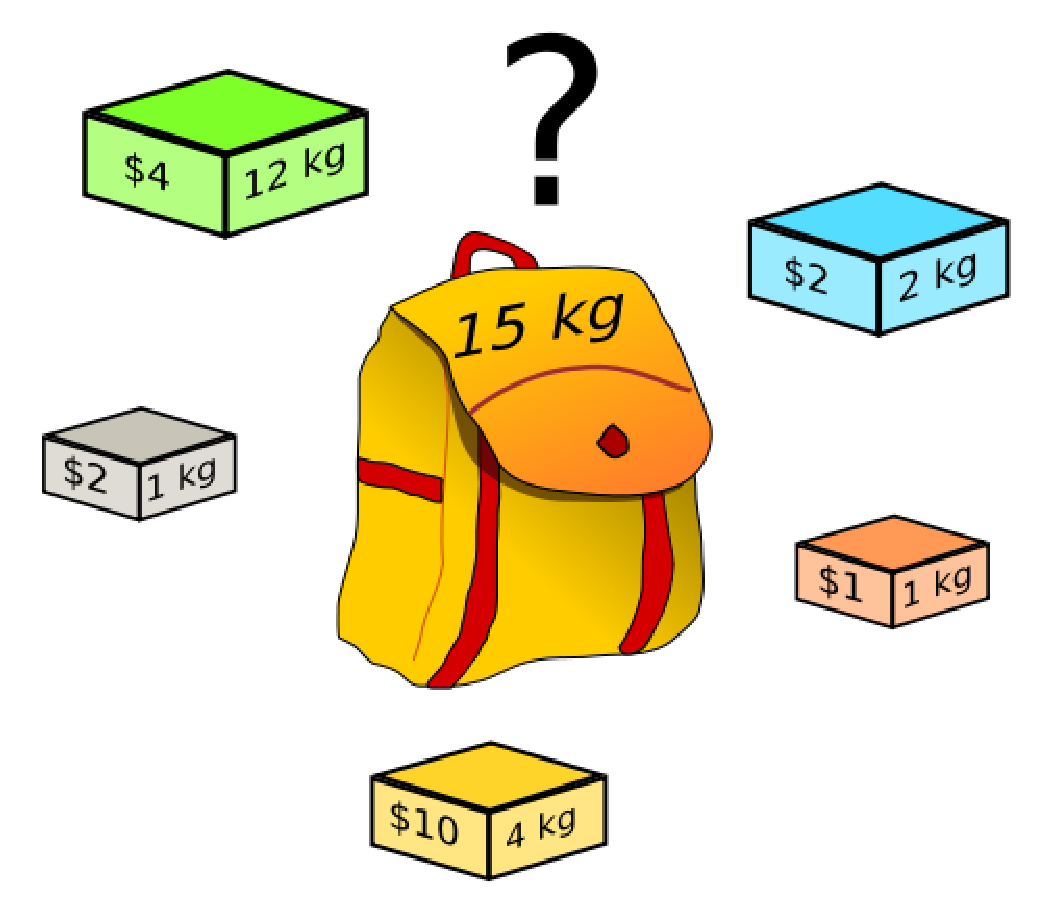
\includegraphics[width=1.5in]{486px-Knapsack.eps}
	\end{figure}
	\end{center}

}

\frame{
\frametitle{{\sc 0-1 Knapsack} problem}


\begin{block}{Formalized Definition:}
{\bf INPUT:} A set of items $S=\{1, 2, ..., n\}$. Item $i$ has weight $w_i$ and value $v_i$. A total weight limit $W$; \\
	{\bf OUTPUT:}  A subset of items to maximize the total value with  total weight below $W$.
\end{block}


\begin{itemize}
\item Here, ``$0-1$'' means that we should select an item (1) or abandon it (0), and we cannot select parts of an item.
\item In contrast, {\sc Fractional Knapsack} problem allow one to select a fractional, say 0.5, of an item. 
\end{itemize}

}




\frame
{
\frametitle{0-1 Knapsack problem: an intuitive algorithm}
	\begin{figure}
	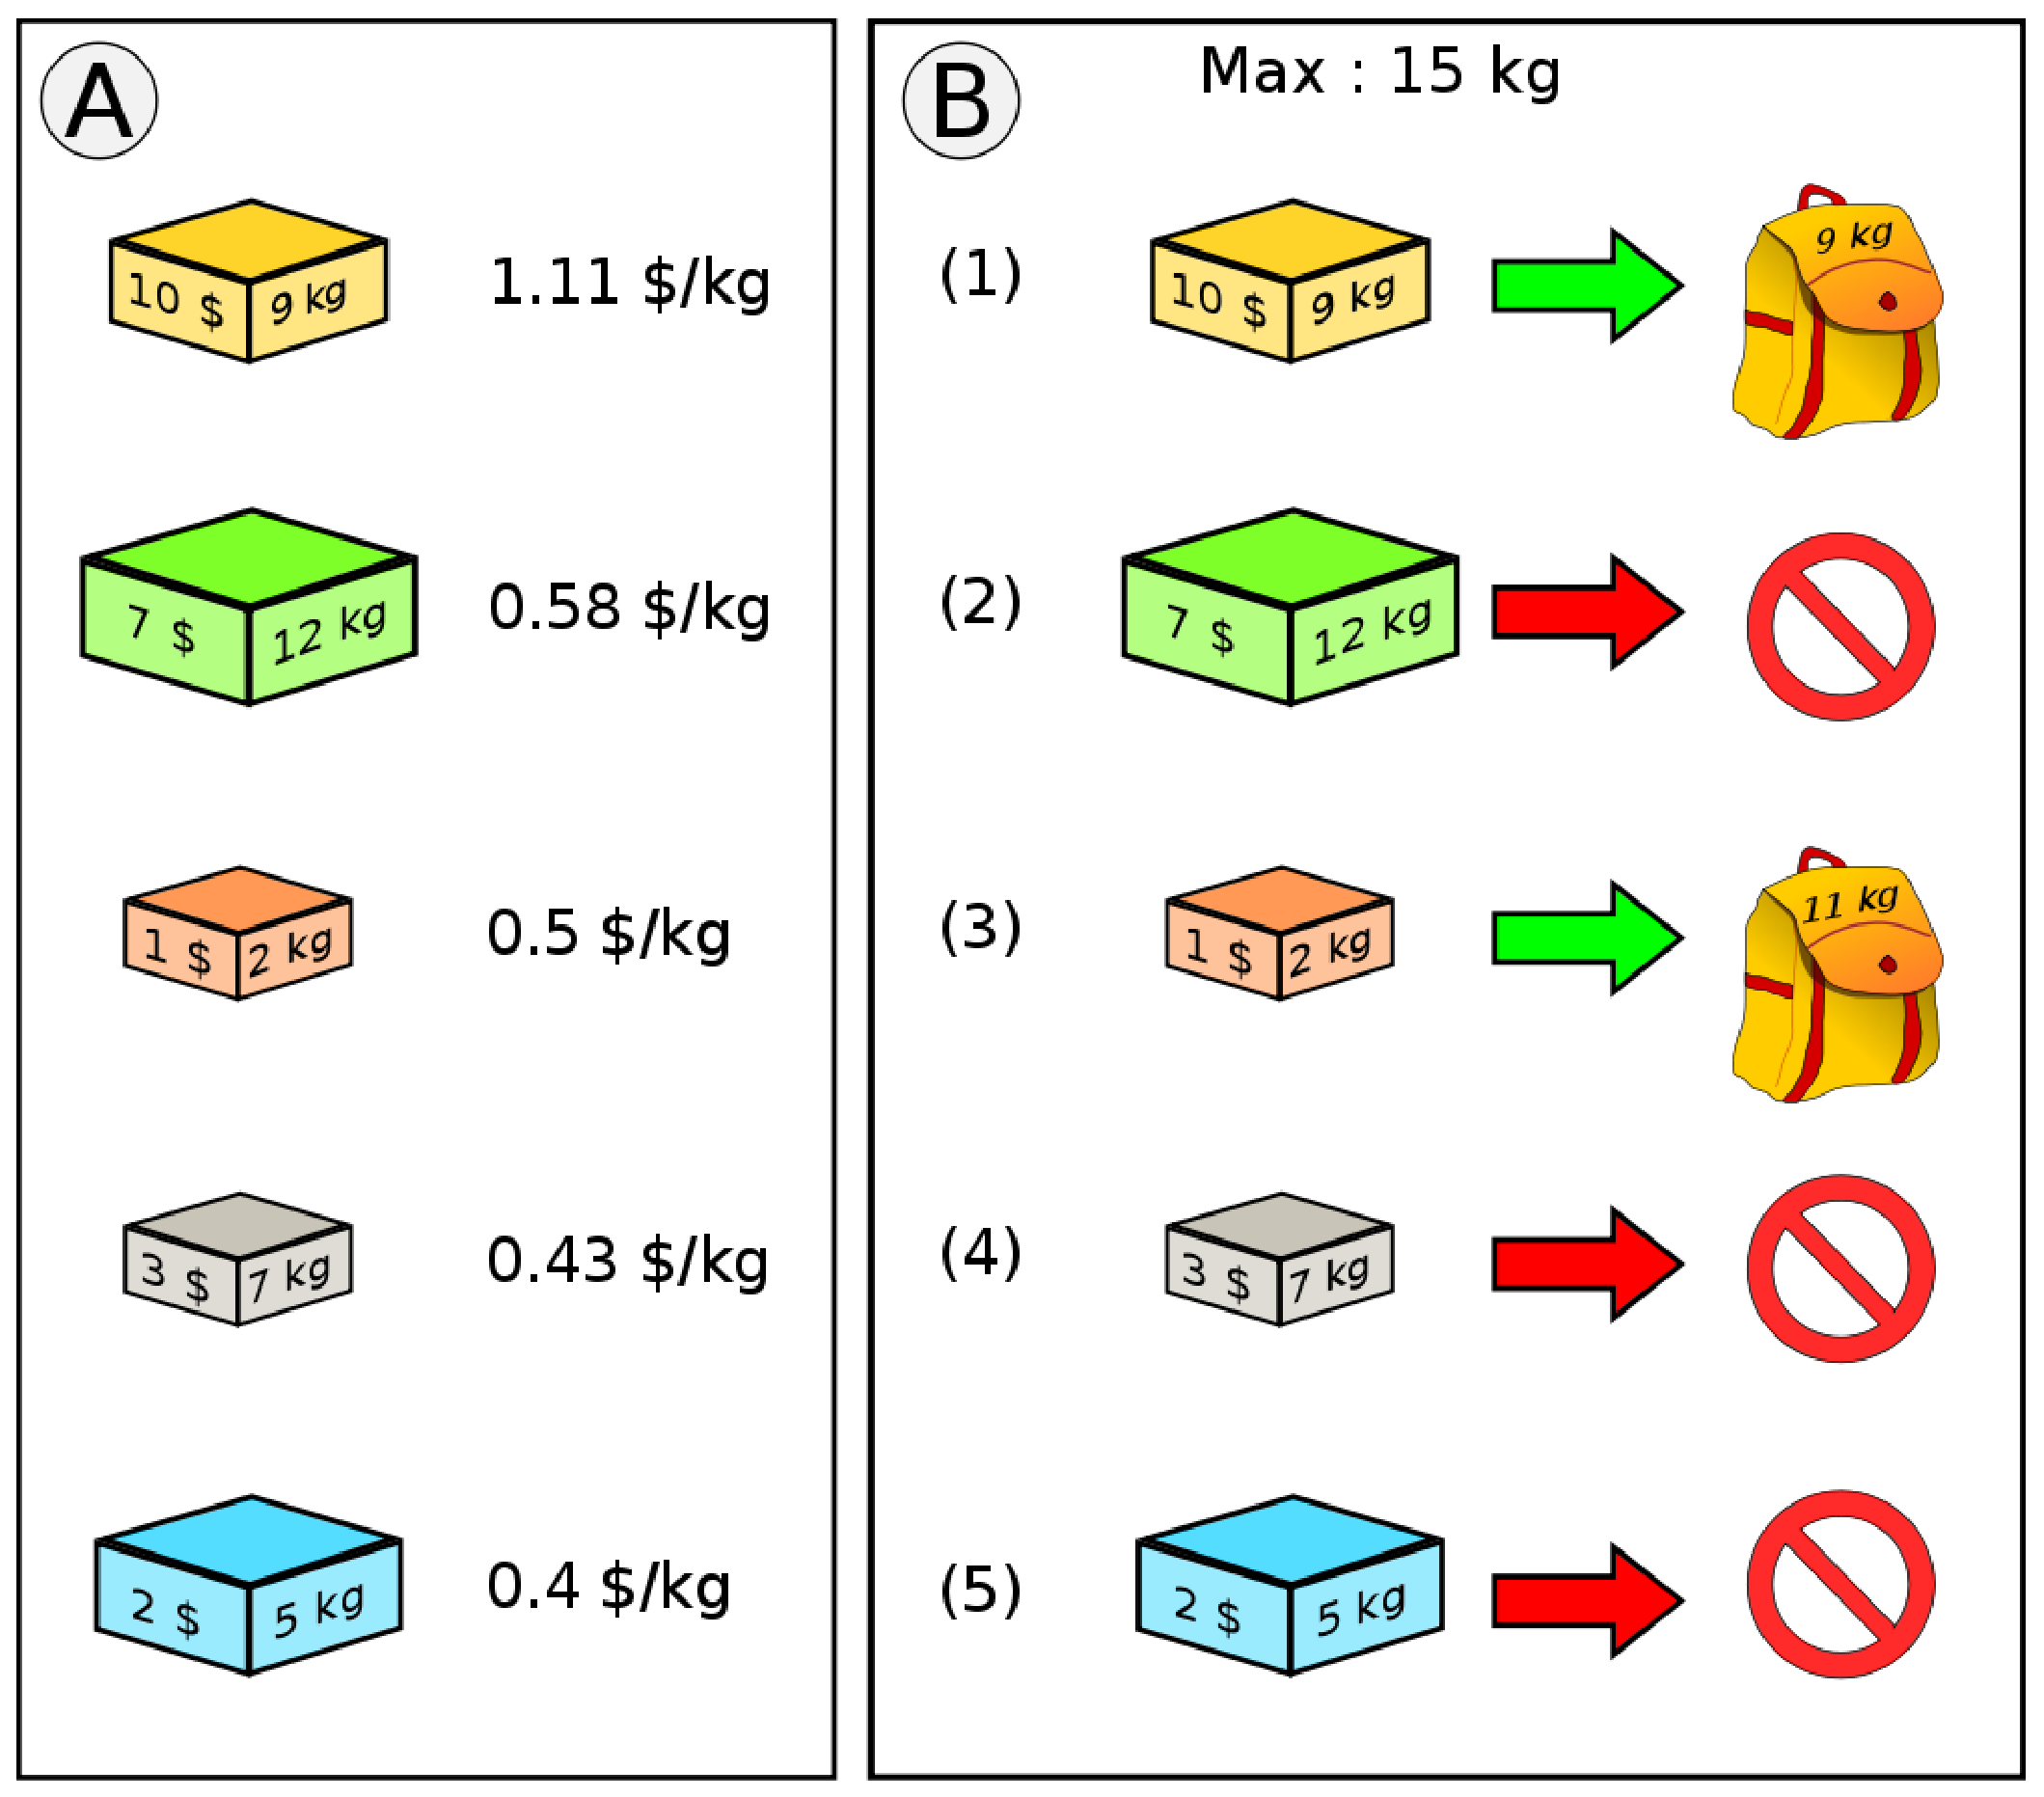
\includegraphics[width=2.3in]{1000px-Knapsack_greedy.eps}
	\end{figure}
  	\begin{itemize}
		\item Intuitive method: selecting ``expensive'' items first.
		\item But this is not the optimal solution. 
	\end{itemize}
%	NP-Completeness: {\sc SubsetSum} $\leq_P$ {\sc Knapsack}. (Hint: simply setting $v_i = w_i$). 
}

 
\frame{
	\frametitle{Defining the general form of sub-problems}
	\begin{itemize}
		\item It is not easy to solve the problem with $n$ items directly. Let's examine whether it is possible to reduce into smaller sub-problems. 
		\item Solution: a subset of items. Let's describe the solving process as a process of \textcolor{red}{\bf multistage  decisions}. At the $i$-th decision stage, we decide whether item $i$ should be selected. 
		\item 
		Let's consider  \textcolor{red}{\bf the first decision}, i.e.  whether the optimal solution contains item $n$ or not (here we assume an order of the items and consider the items from end to beginning). This decision has two options: 
		\begin{enumerate}
		\item {\sc Select}: Then it suffices to select items as ``expensive'' as possible from $\{1,2,...,n-1\}$ with weight limit $W-w_n$.
		\item {\sc Abandon}: Otherwise, we should select items as ``expensive'' as possible from $\{1,2,...,n-1\}$ with weight limit $W$.
		\end{enumerate}
		\item In both cases, the original problem is reduced into smaller sub-problems. 
%	\begin{figure}
%	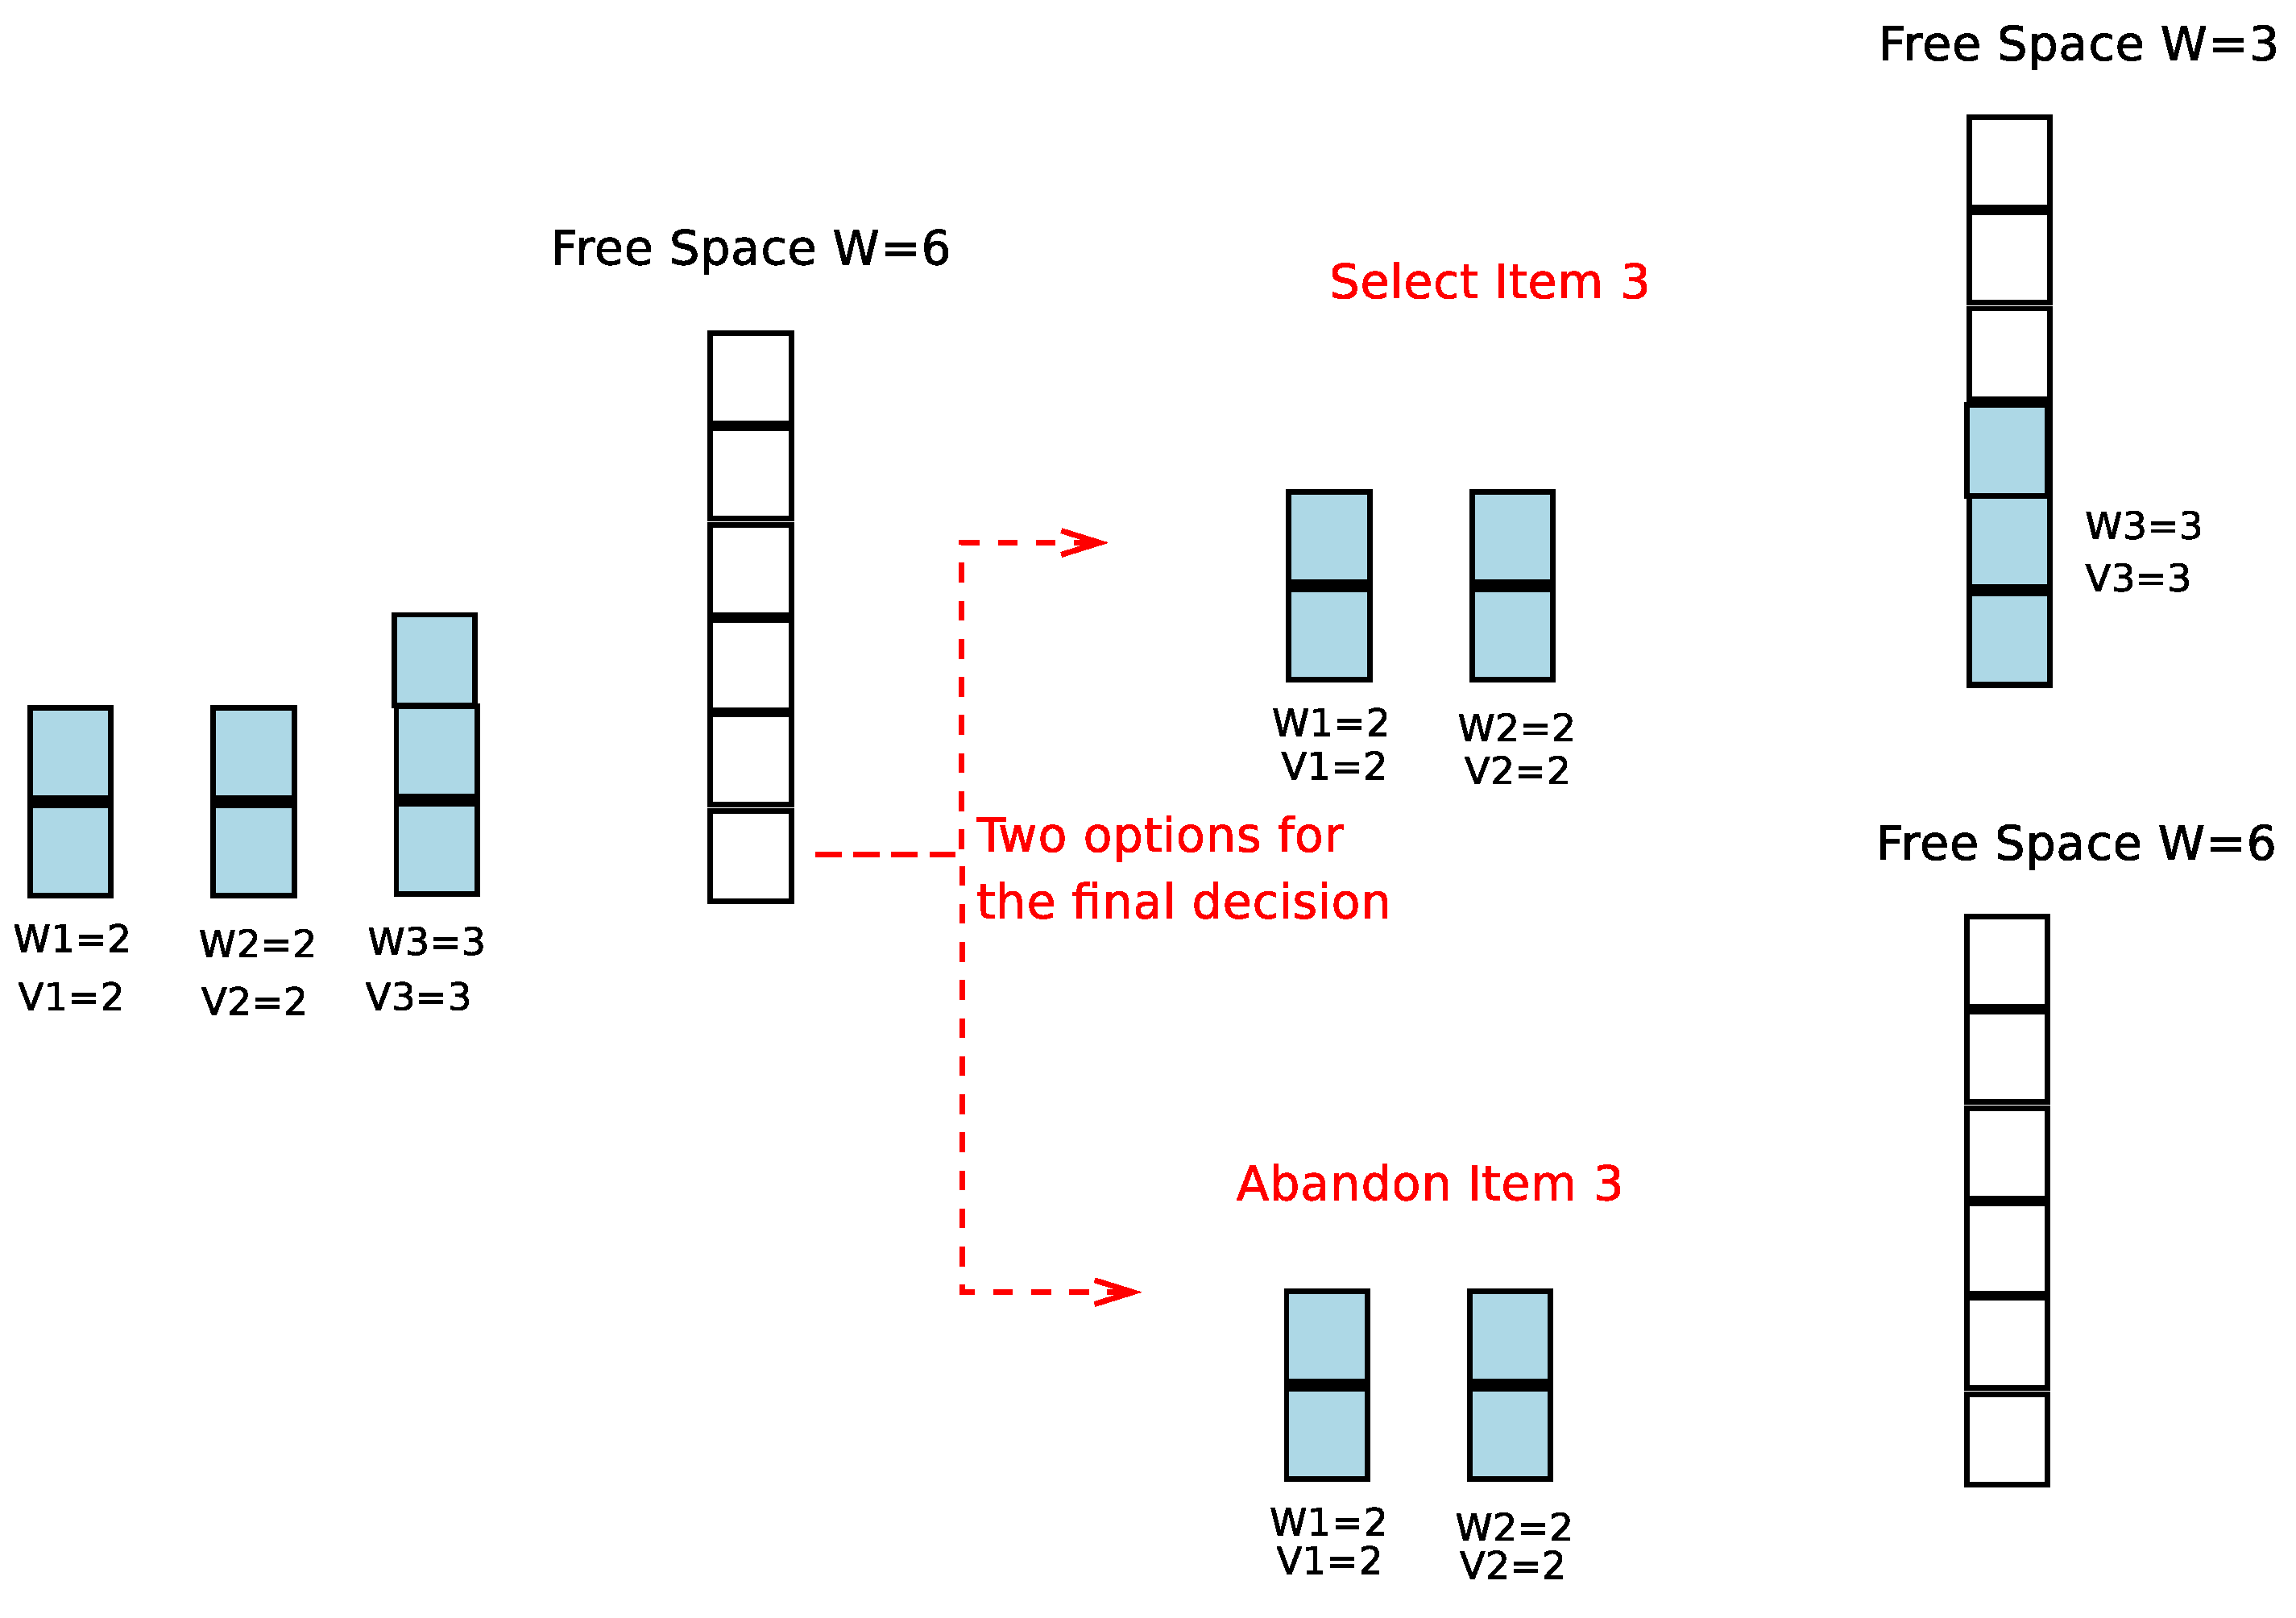
\includegraphics[width=2.3in]{L6-Knapsackexample.eps}
%	\end{figure}
	\end{itemize}
}

\frame{
	\frametitle{Optimal sub-structure property}
	\begin{itemize}
		\item Summarizing these two cases, we can set the general form of sub-problems as: to select items as ``expensive'' as possible from $\{1,2,...,i\}$ with weight limit $w$. Denote the optimal solution value as $OPT(\{1, 2, ..., i\}, w)$.
		\item Then we can prove the optimal sub-structure property: 	
\begin{footnotesize}
\[
OPT(\{1, 2, ..., n\}, W) = \max\begin{cases}
	OPT(\{1, 2, ..., n-1\}, W) \nonumber \\ 
	OPT(\{1, 2, ..., n-1\}, W-w_{n}) + v_{n} \nonumber
\end{cases}
\]
 \end{footnotesize}		
%		
%		\begin{small}	
%		$OPT( n, W )=\max\{OPT(n-1, W), OPT(n-1, W-w_n) + v_n\}$
%		\end{small}
%	\begin{figure}
%		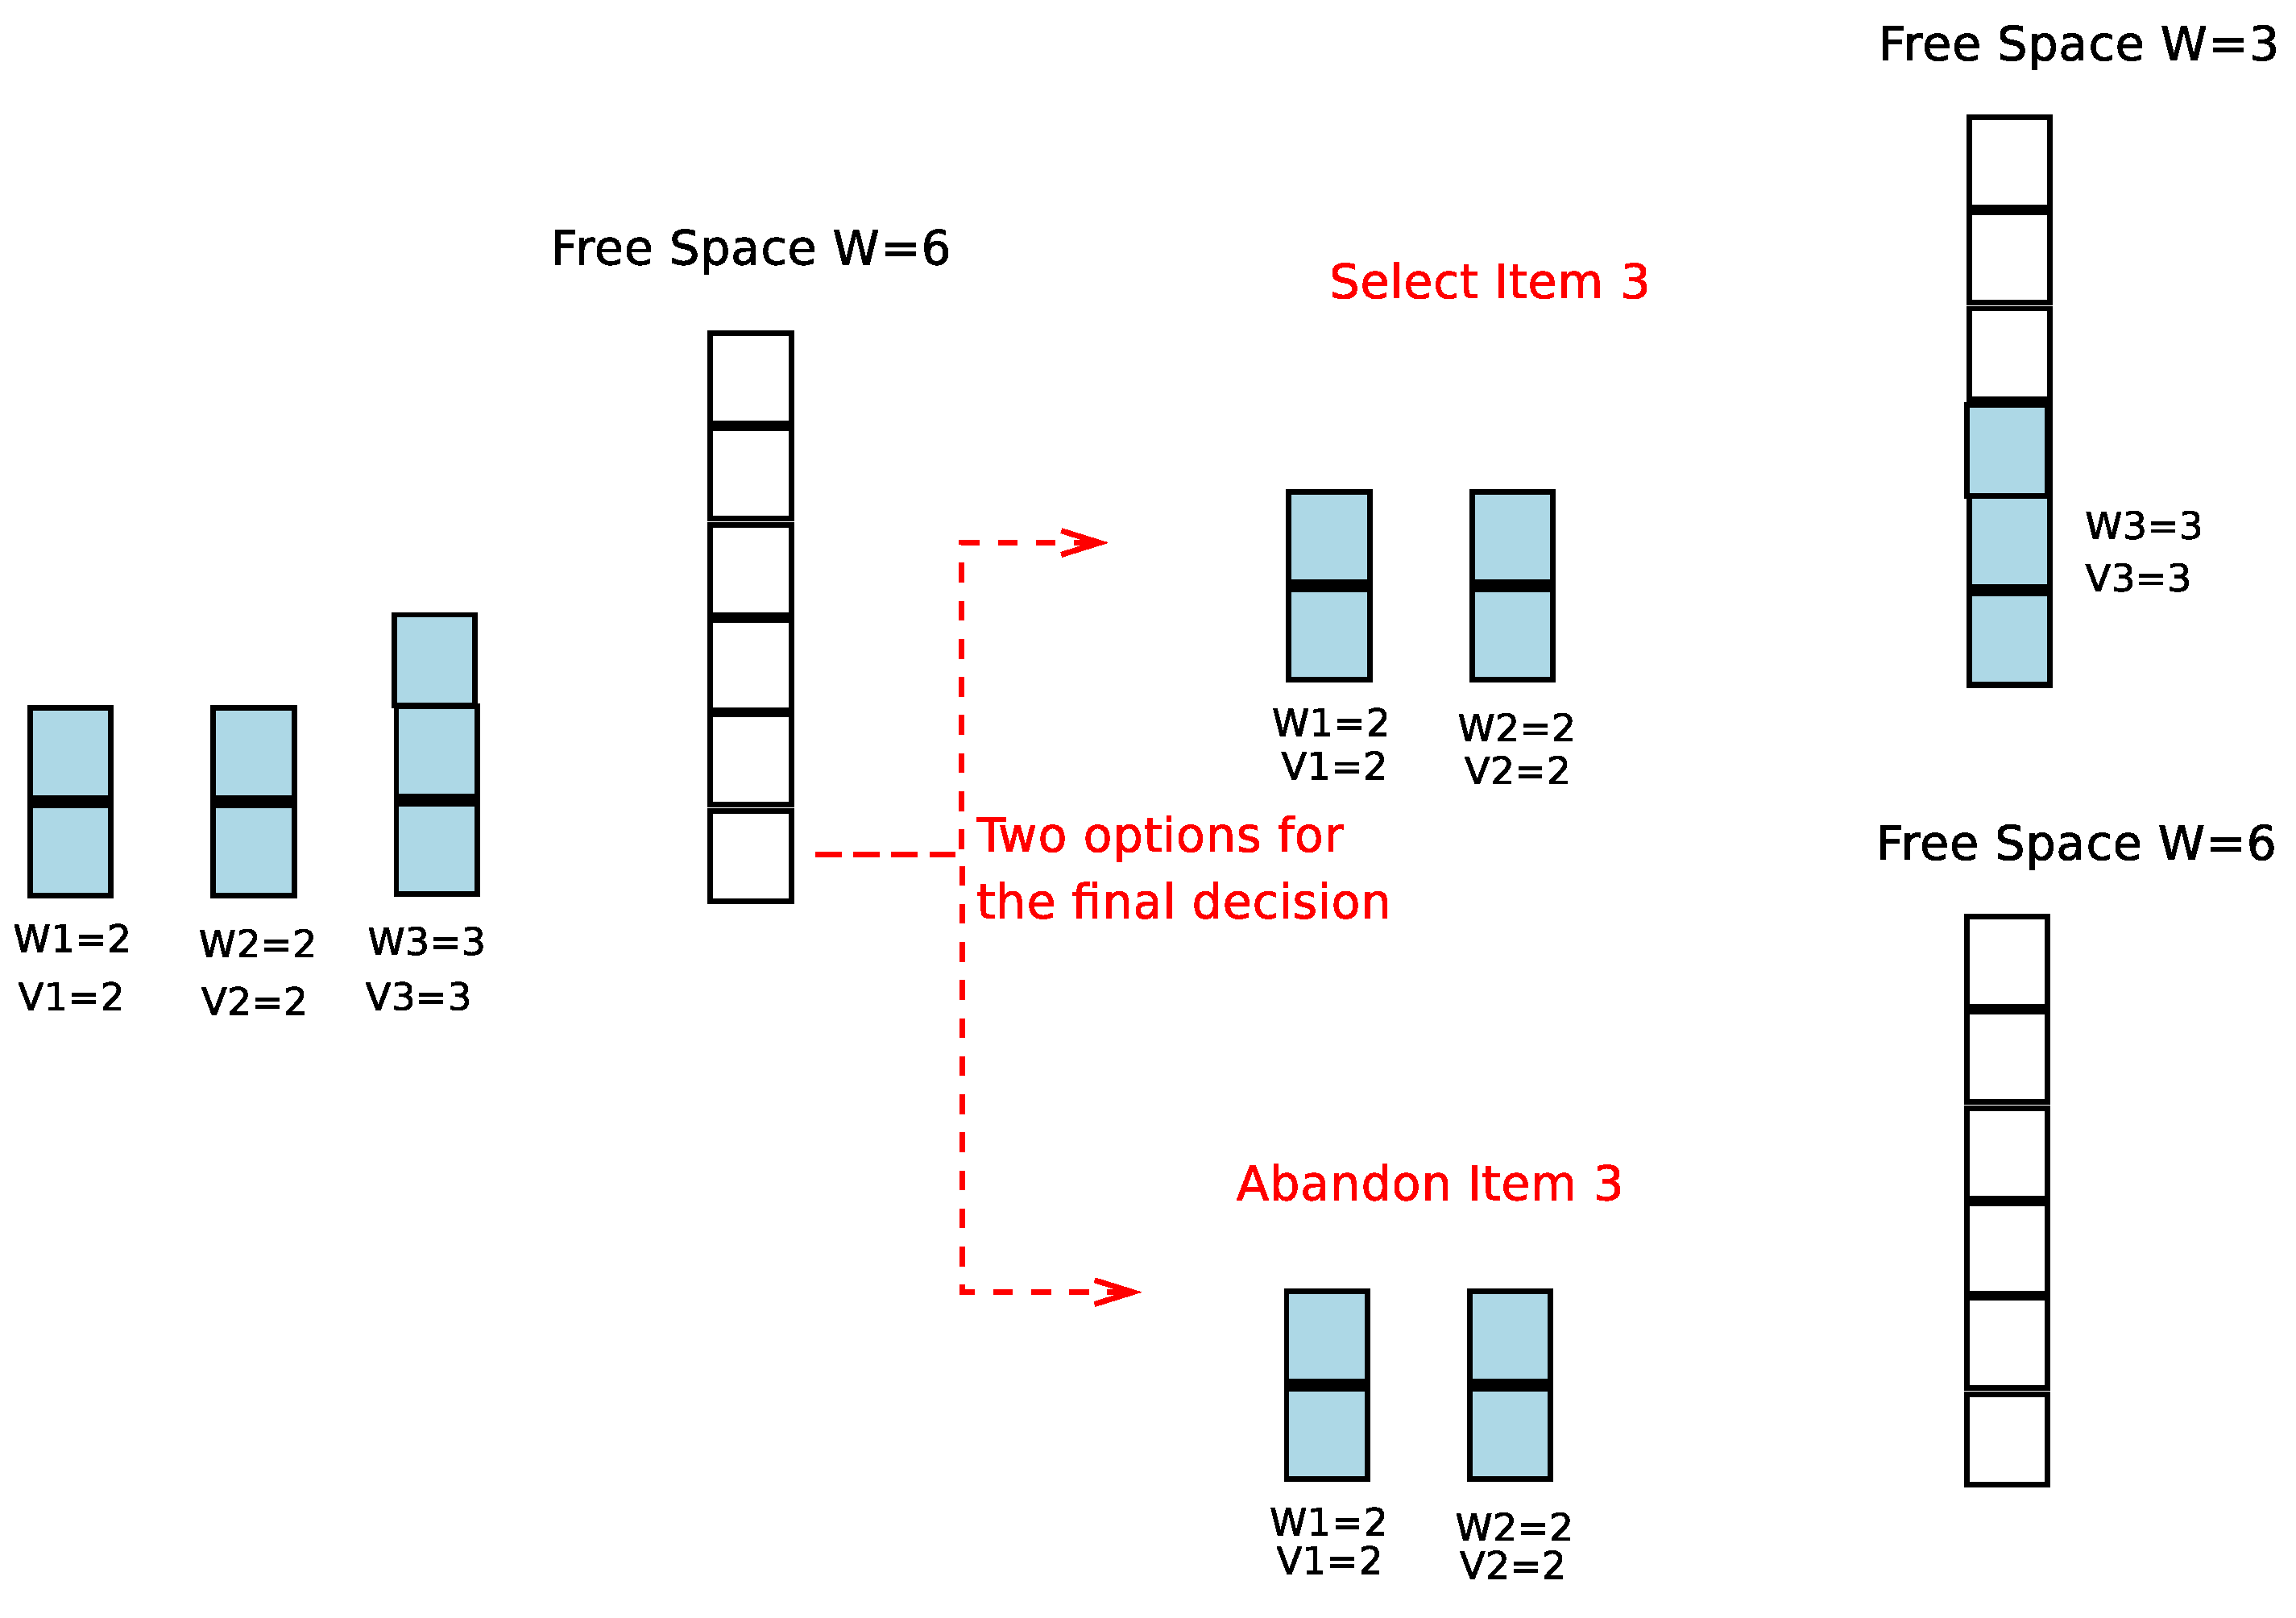
\includegraphics[width=2.6in]{L6-Knapsackexample.eps}
%	\end{figure}
\end{itemize}
}


\frame{
\frametitle{Algorithm}
{\sc Knapsack}$(n, W)$
\begin{algorithmic}[1]
\FOR{$w=1$ to $W$ }
	\STATE $OPT[0, w] = 0$;
\ENDFOR
\FOR{$i=1$ to $n$ }
	\FOR{$w=1$ to $W$ }
		\STATE $OPT[i,w] = \max \{OPT[i-1, w], v_i+OPT[i-1, w-w_i]\}$;
	\ENDFOR
\ENDFOR
\RETURN{$OPT[n, W]$};
\end{algorithmic}

\begin{itemize}
	\item Here we use $OPT[i, w]$ to represent $OPT(\{1, 2, ..., i\}, w)$ for simplicity.  
\end{itemize}
}


\frame{
	\frametitle{An example: Step 1}

\begin{figure}
    
\begin{tikzpicture}[scale=0.9, auto,swap]

  
  	\def\d{0.5};
 	\def\dy{0};
	\def\dx{0};
         	\draw[  thick, fill=blue!20 ] (0 + \dx,  0 + \dy) rectangle (0 + \dx + \d,  0 + \dy + 2*\d);
	\node at (0.5*\d+\dx, -0.5+\dy) {\tiny $w_1=2$}; 
	\node at (0.5*\d+\dx, -0.8+\dy) {\tiny $v_1=2$}; 
	
	\def\dx{1.5};
         	\draw[  thick, fill=blue!20 ] (0 + \dx,  0 + \dy) rectangle (0 + \dx + \d,  0 + \dy + 2*\d);
	\node at (0.5*\d+\dx, -0.5+\dy) {\tiny $w_2=2$}; 
	\node at (0.5*\d+\dx, -0.8+\dy) {\tiny $v_2=2$}; 
	
	\def\dx{3};
         	\draw[  thick, fill=blue!20 ] (0 + \dx,  0 + \dy) rectangle (0 + \dx + \d,  0 + \dy + 3*\d);
	\node at (0.5*\d+\dx, -0.5+\dy) {\tiny $w_3=3$}; 
	\node at (0.5*\d+\dx, -0.8+\dy) {\tiny $v_3=3$}; 
	
	
	\def\dx{4.5};
         	\draw[  thick, fill=white ] (0 + \dx,  0 + \dy) rectangle (0 + \dx + \d,  0 + \dy + 6*\d);
	\node at (0.5*\d+\dx, -0.5+\dy) {\tiny $W=6$}; 
	

\end{tikzpicture}
\end{figure}


\begin{figure}[!ht]
  \centering
  \begin{minipage}[c]{0.45\linewidth}
    \makebox[10ex][s]{Initially all $OPT[0,w]=0$}
  \end{minipage}
  \begin{minipage}[c]{0.45\linewidth}
    %\centering
    %\begin{table}
      %\entering
      \begin{tabular}{c|c|c|c|c|c|c|c|}
        \multicolumn{1}{r}{$w=$}& \multicolumn{1}{c}{0} & \multicolumn{1}{c}{1} & \multicolumn{1}{c}{2} & \multicolumn{1}{c}{3} & \multicolumn{1}{c}{4} & \multicolumn{1}{c}{5} & \multicolumn{1}{c}{6}\\
        \hhline{~-------}
        $i=3$ &  &  &  &  &  &  &  \\
        \hhline{~-------}
        $i=2$ &  &  &  &  &  &  &     \\
        \hhline{~-------}
        $i=1$ &  &  &  &  &  &  &     \\
        \hhline{~-------}
        $i=0$ & 0 & 0 & 0 & 0 & 0 & 0 & 0 \\
        \hhline{~-------}
      \end{tabular}
  \end{minipage}
\end{figure}
}

\frame{
	\frametitle{Step 2}

\begin{figure}[!ht]
  \centering
  \begin{minipage}[c]{0.45\linewidth}
    $OPT[1,2]=\max\{\\ \hspace*{.5cm}OPT[0,2](=0),\\ \hspace*{.5cm}OPT[0,0]+V_1(=0+2)\}$\\ \hspace*{1.7cm}$=2$
    %\parbox{OPT[1,2]=max\{\\OPT[0,2](=0),\\~~OPT[0,0]+V1(=0+2)\}\\~~=2}
  \end{minipage}
  \begin{minipage}[c]{0.45\linewidth}
    \centering
    %\begin{table}[!ht]
      \centering
      \begin{tabular}{c|c|c|c|c|c|c|c|}
        \multicolumn{1}{r}{$w=$}& \multicolumn{1}{c}{0} & \multicolumn{1}{c}{1} & \multicolumn{1}{c}{2} & \multicolumn{1}{c}{3} & \multicolumn{1}{c}{4} & \multicolumn{1}{c}{5} & \multicolumn{1}{c}{6}\\
        \hhline{~-------}
        $i=3$ &  &  &  &  &  &  &  \\
        \hhline{~-------}
        $i=2$ &  &  &  &  &  &  &     \\
        \hhline{~-------}
        $i=1$ & 0 & 0 & 2 & 2 & 2 & 2 & 2    \\
        \hhline{~-------}
        $i=0$ & 0 & 0 & 0 & 0 & 0 & 0 & 0 \\
        \hhline{~-------}
      \end{tabular}
      \begin{tikzpicture}[overlay]
      \draw[red, line width=1pt] (0.35,0.8) circle (0.25cm);
      \draw[->,red, line width=1pt] (-0.8,0.3) -- (0.10,0.8);
      \draw[->,red, line width=1pt] (0.6,0.15) -- (0.6,0.6);
      \end{tikzpicture}
    %\end{table}
  \end{minipage}
\end{figure}
}

\frame{
	\frametitle{Step 3}

\begin{figure}[!ht]
  \centering
  \begin{minipage}[c]{0.45\linewidth}
    $OPT[2,4]=\max\{\\ \hspace*{.5cm}OPT[1,4](=2),\\ \hspace*{.5cm}OPT[1,2]+V_2(=2+2)\}$\\ \hspace*{1.7cm}$=4$
  \end{minipage}
  \begin{minipage}[c]{0.45\linewidth}
    \centering
    %\begin{table}[!ht]
      \centering
      \begin{tabular}{c|c|c|c|c|c|c|c|}
        \multicolumn{1}{r}{$w=$}& \multicolumn{1}{c}{0} & \multicolumn{1}{c}{1} & \multicolumn{1}{c}{2} & \multicolumn{1}{c}{3} & \multicolumn{1}{c}{4} & \multicolumn{1}{c}{5} & \multicolumn{1}{c}{6}\\
        \hhline{~-------}
        $i=3$ &  &  &  &  &  &  &  \\
        \hhline{~-------}
        $i=2$ & 0 & 0 & 2 & 2 & 4 & 4 & 4    \\
        \hhline{~-------}
        $i=1$ & 0 & 0 & 2 & 2 & 2 & 2 & 2    \\
        \hhline{~-------}
        $i=0$ & 0 & 0 & 0 & 0 & 0 & 0 & 0 \\
        \hhline{~-------}
      \end{tabular}
      \begin{tikzpicture}[overlay]
      \draw[red, line width=1pt] (1.6,1.3) circle (0.25cm);
      \draw[->,red, line width=1pt] (.6,.75) -- (1.3,1.3);
      \draw[->,red, line width=1pt] (1.85,.6) -- (1.85,1.1);
      \end{tikzpicture}
    %\end{table}
  \end{minipage}
\end{figure}
}

\frame{
	\frametitle{Step 4}

\begin{figure}[!ht]
  \centering
  \begin{minipage}[c]{0.45\linewidth}
    $OPT[3,3]=\max\{\\ \hspace*{.5cm}OPT[2,3](=2),\\ \hspace*{.5cm}OPT[2,0]+V_3(=0+3)\}$\\ \hspace*{1.7cm}$=3$
  \end{minipage}
  \begin{minipage}[c]{0.45\linewidth}
    \centering
    %\begin{table}[!ht]
      \centering
      \begin{tabular}{c|c|c|c|c|c|c|c|}
        \multicolumn{1}{r}{$w=$}& \multicolumn{1}{c}{0} & \multicolumn{1}{c}{1} & \multicolumn{1}{c}{2} & \multicolumn{1}{c}{3} & \multicolumn{1}{c}{4} & \multicolumn{1}{c}{5} & \multicolumn{1}{c}{6}\\
        \hhline{~-------}
        $i=3$ & 0 & 0 & 2 & 3 & 4 & 5 & 5 \\
        \hhline{~-------}
        $i=2$ & 0 & 0 & 2 & 2 & 4 & 4 & 4    \\
        \hhline{~-------}
        $i=1$ & 0 & 0 & 2 & 2 & 2 & 2 & 2    \\
        \hhline{~-------}
        $i=0$ & 0 & 0 & 0 & 0 & 0 & 0 & 0 \\
        \hhline{~-------}
      \end{tabular}
      \begin{tikzpicture}[overlay]
      \draw[red, line width=1pt] (1.0,1.8) circle (0.25cm);
      \draw[->,red, line width=1pt] (-0.8,1.3) -- (0.7,1.8);
      \draw[->,red, line width=1pt] (1.2,1.15) -- (1.2,1.60);
      \end{tikzpicture}
    %\end{table}
  \end{minipage}
\end{figure}
}

\frame{
	\frametitle{Backtracking}


\begin{figure}[!ht]
  \centering
  \begin{minipage}[c]{0.45\linewidth}
    
    $OPT[3,6]=\max\{\\ \hspace*{.5cm}OPT[2,6](=4),\\ \hspace*{.5cm}OPT[2,3]+V_3(=2+3)\}$\\ \hspace*{1.7cm}$=5$\\
    Decision: Select item 3\\


    $OPT[2,3]=\max\{\\ \hspace*{.5cm}OPT[1,3](=2),\\ \hspace*{.5cm}OPT[1,1]+V_2(=0+2)\}$\\ \hspace*{1.7cm}$=2$\\
    Decision: Select item 2

  \end{minipage}
  \begin{minipage}[c]{0.45\linewidth}
    \centering
    %\begin{table}[!ht]
      \centering
      \begin{tabular}{r|c|c|c|c|c|c|c|}
        \multicolumn{1}{r}{$w=$}& \multicolumn{1}{c}{0} & \multicolumn{1}{c}{1} & \multicolumn{1}{c}{2} & \multicolumn{1}{c}{3} & \multicolumn{1}{c}{4} & \multicolumn{1}{c}{5} & \multicolumn{1}{c}{6}\\
        \hhline{~-------}
        $i=3$ & 0 & 0 & 2 & 3 & 4 & 5 & 5 \\
        \hhline{~-------}
        $i=2$ & 0 & 0 & 2 & 2 & 4 & 4 & 4    \\
        \hhline{~-------}
        $i=1$ & 0 & 0 & 2 & 2 & 2 & 2 & 2    \\
        \hhline{~-------}
        $i=0$ & 0 & 0 & 0 & 0 & 0 & 0 & 0 \\
        \hhline{~-------}
      \end{tabular}
      \begin{tikzpicture}[overlay]
      \draw[red, line width=1pt] (2.8,1.8) circle (0.25cm);
      \draw[red, line width=1pt] (0.97,1.3) circle (0.25cm);
      \draw[->,red, line width=1pt] (2.55,1.8) -- (1.25,1.32);

      \draw[red, line width=1pt] (-0.275,0.8) circle (0.25cm);
      \draw[->,red, line width=1pt] (0.67, 1.2) -- (-0.08, 0.9);
      
      \end{tikzpicture}
    %\end{table}
  \end{minipage}
\end{figure}
}

%
%\frame[allowframebreaks]{
%\frametitle{Example}
%
%	\begin{figure}
%	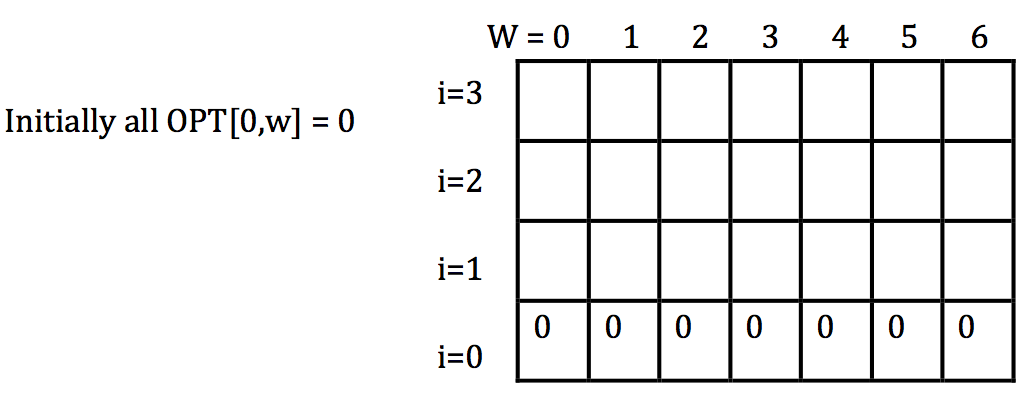
\includegraphics[width=4in]{L5-Knapsackalgostep1.png}
%	\end{figure}
%	\begin{figure}
%	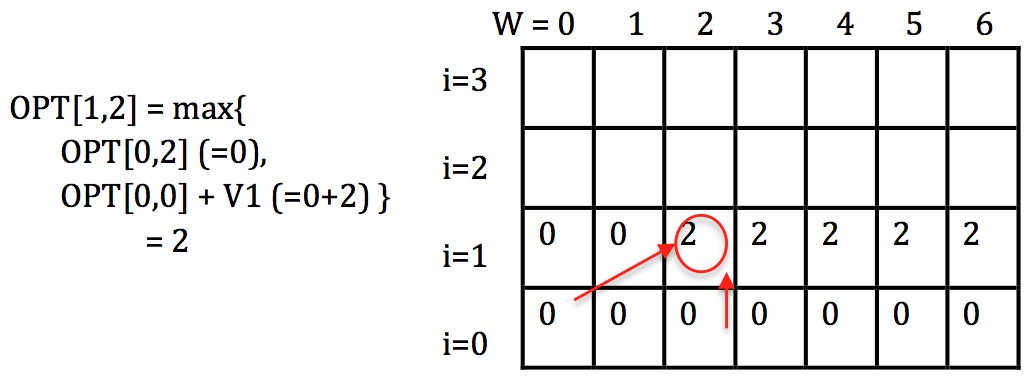
\includegraphics[width=4in]{L5-Knapsackalgostep2.png}
%	\end{figure}	
%	\begin{figure}
%	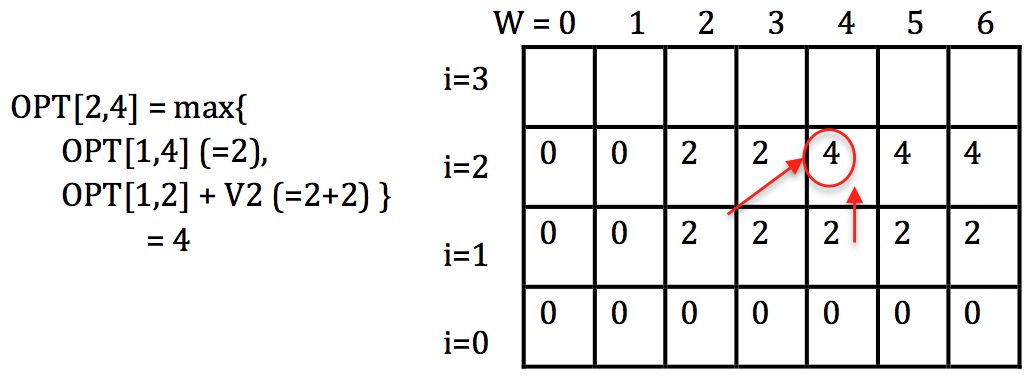
\includegraphics[width=4in]{L5-Knapsackalgostep3.png}
%	\end{figure}	
%	\begin{figure}
%	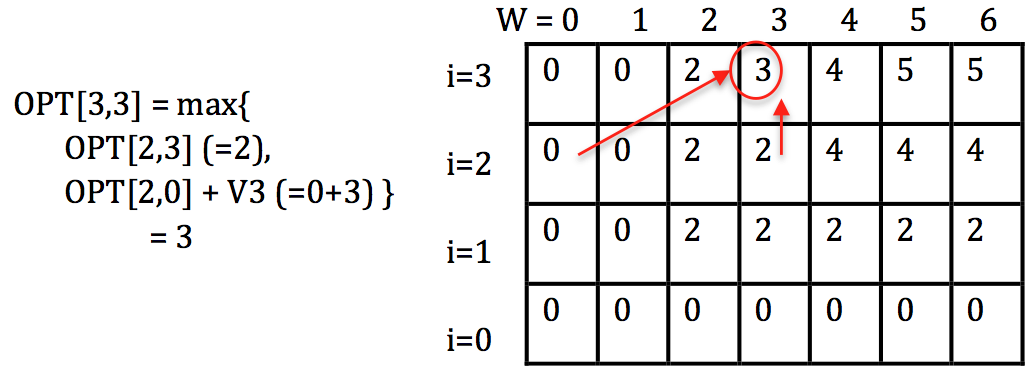
\includegraphics[width=4in]{L5-Knapsackalgostep4.png}
%	\end{figure}
%}
%
%\frame{
%\frametitle{Backtracking: step 1}
%	\begin{figure}
%	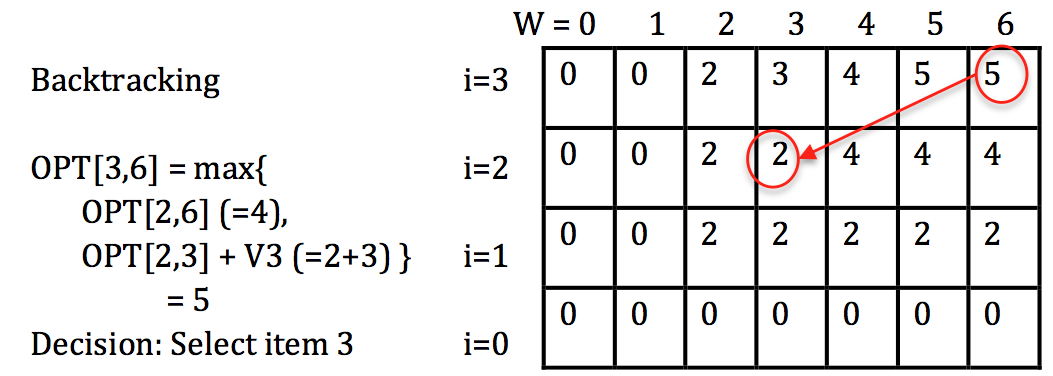
\includegraphics[width=4in]{L5-Knapsackalgobacktrackstep1.png}
%	\end{figure}
%}
%
%\frame{
%\frametitle{Backtracking: step 2}
%	\begin{figure}
%	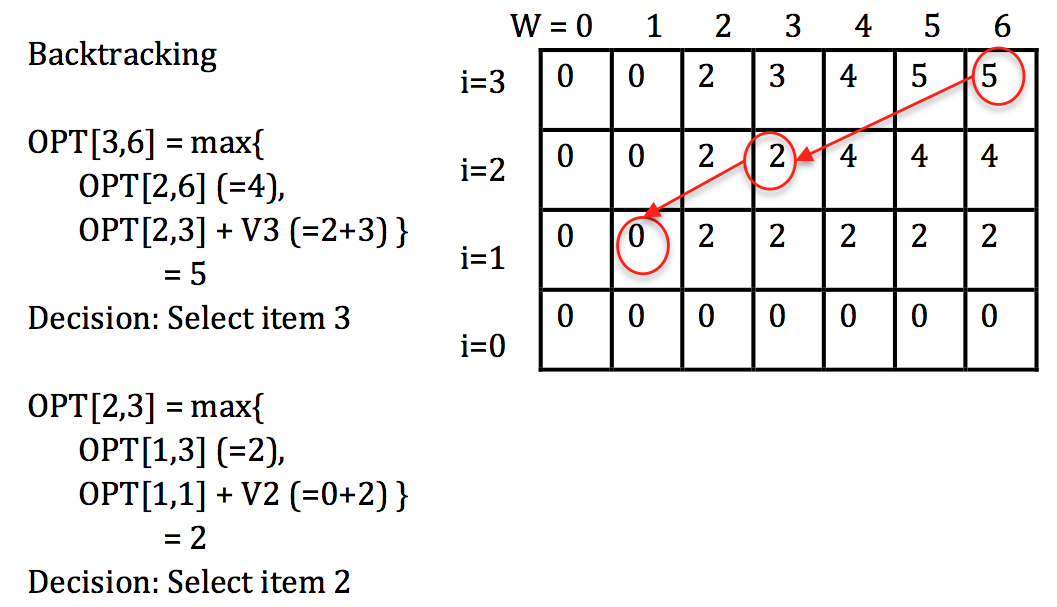
\includegraphics[width=4in]{L5-Knapsackalgobacktrackstep2.png}
%	\end{figure}
%}

\frame{
\frametitle{Time complexity analysis}
\begin{itemize}
 \item Time complexity: $O(nW)$. (Hint: for each entry in the matrix, only a comparison is needed;  we have $O(nW)$ entries in the matrix.)
\item Notes: 
	\begin{enumerate}
	% \item $W$ should be integer. (Why? Otherwise, we cannot construct an array $OPT[1..W, 1..n]$)
	 \item This algorithm is inefficient when $W$ is large, say $W=1M$.
	\item Remember that a polynomial time algorithm costs time polynomial in the \textcolor{red}{\bf input length}. However, this algorithm costs time $mW=m2^{\log W}=m2^{\text{input length} }$. Exponential!
	 \item Pseudo-polynomial time algorithm: polynominal in the \textcolor{red}{\bf value} of $W$ rather than the \textcolor{red}{\bf length} of $W$ ($\log W$). 
	\item We will revisit this algorithm in approximation algorithm design. 
	\end{enumerate}
\end{itemize}
}


\frame{
	\frametitle{Why should we consider items from end to beginning? } 

\begin{itemize}    
\item 
Let's examine the following two types of selection of items: 
\begin{enumerate}
 \item 
 If we consider an arbitrary item $i$, then the sub-problem becomes into ``selecting items as expensive as possible from \textcolor{red}{\bf a subset $s$} with weight limit $w$''.  We have the following recursion: 
 \begin{footnotesize}
\[
OPT(\{1, 2, ..., n\}, W) = \max\begin{cases} OPT(\{1, 2, ..., n\} - \{i\}, W) \nonumber \\
	OPT(\{1, 2, ..., n\} - \{i\}, W-w_{i}) + v_{i} \nonumber
	\end{cases}
\]
 \end{footnotesize}

 
\item
In contrast, if we assume an order of the items and consider them from end to beginning, then the subproblem can be set as ``selecting items as expensive as possible from $\{1,2,...,i\}$ with weight limit $w$'' and we have the following recursion: 
 \begin{footnotesize}
\[
OPT(\{1, 2, ..., n\}, W) = \max\begin{cases}
	OPT(\{1, 2, ..., n-1\}, W) \nonumber \\ 
	OPT(\{1, 2, ..., n-1\}, W-w_{n}) + v_{n} \nonumber
\end{cases}
\]
 \end{footnotesize}
\end{enumerate} 
\item In fact, the first one exploits  \textcolor{red}{\bf recursion over sets}, which leads to an exponential number of subproblems. In contrast,  the second one is a \textcolor{red}{\bf recursion over sequences} and the number of subproblems is only $O(nW)$.  
\end{itemize}

%The Subset-Sum($n$,$W$) Algorithm, using dynamic programming, correctly computes the optimal value of the problem, and runs in $O$($nW$) time. The problem is $NP$-hard and the algorithm is \emph{pseudo-polynomial}.
		%\item We can design an improved algorithm, using approximation.
}

\frame{
	\frametitle{Extension: The first public-key encryption system} 
	\begin{itemize}
		\item {\it Cryptosystems based on the knapsack problem were among the first public key systems to be
invented, and for a while were considered to be among the most promising. However, essentially
all of the knapsack cryptosystems that have been proposed so far have been broken. These notes
outline the basic constructions of these cryptosystems and attacks that have been developed on
them. } 	\end{itemize}	 
	
	See {\it The Rise and Fall of Knapsack Cryptosystems} for details.

}

\frame{
\begin{block}{}
 	{\sc Vertex Cover}: recursion over \textcolor{red}{\bf trees} 
\end{block}
}


\frame{
\frametitle{{\sc Vertex Cover } Problem }

\begin{itemize}
 \item 
Practical problem: \\ {\em 
Given $n$ sites connected with paths, how many guards (or cameras)  should be deployed on sites to surveille {\bf all} the paths?}

\begin{block}{Formalized Definition:}
 {\bf Input:} Given a graph $G=<V,E>$\\
 {\bf Output:} the minimum of nodes $S  \subseteq V$, such that each edge has at least one of its endpoints in $S$ 
\end{block}

\item For example,  how many nodes are needed to cover all edges in the following graph? 

\begin{figure}
\begin{tikzpicture}[scale=1.1, auto,swap]
    % Draw a 7,11 network
    % First we draw the vertices
    \foreach \pos/\name in {{(0,2)/v1}, {(2,2)/v2}, {(1,1)/v3}, {(2,1)/v4}, {(3,1)/v5}, {(0,0)/v6}, {(2,0)/v7}}
        \node[smallvertex] (\name) at \pos {};
        
    % Connect vertices with edges and draw weights
    \foreach \source/ \dest /\weight in {v1/v2/{}, v1/v3/{}, v2/v3/{}, v2/v4/{}, v2/v5/{}, v3/v6/{}, v3/v7/{}, v6/v7/{}, v4/v7/{}, v5/v7/{}  }
        \path[undirectededge] (\source) -- node[weight] {\small $\weight$} (\dest);
%       \draw[dashed, ->] (0,0) arc  (120:60:2);

      \end{tikzpicture}

\end{figure}

\end{itemize} 

} 

\frame{
\frametitle{Vertex cover} 

\begin{figure}
\begin{tikzpicture}[scale=1.1, auto,swap]
    % Draw a 7,11 network
    % First we draw the vertices
    \foreach \pos/\name in {{(0,2)/v1}, {(2,2)/v2}, {(1,1)/v3}, {(2,1)/v4}, {(3,1)/v5}, {(0,0)/v6}, {(2,0)/v7}}
        \node[smallvertex] (\name) at \pos {};
        
    % Connect vertices with edges and draw weights
    \foreach \source/ \dest /\weight in {v1/v2/{}, v1/v3/{}, v2/v3/{}, v2/v4/{}, v2/v5/{}, v3/v6/{}, v3/v7/{}, v6/v7/{}, v4/v7/{}, v5/v7/{}  }
        \path[undirectededge] (\source) -- node[weight] {\small $\weight$} (\dest);
%       \draw[dashed, ->] (0,0) arc  (120:60:2);

%    \foreach \pos/\name in {{(1,1)/v3}, {(2,1)/v4}, {(3,1)/v5}}
%        \node[blue smallvertex] (\name) at \pos {};

    \foreach \pos/\name in {{(1,1)/v3}, {(2,2)/v2},  {(2,0)/v7}}
        \node[red smallvertex] (\name) at \pos {};
      \end{tikzpicture}

\end{figure}

\begin{itemize}
\item The nodes in red form a vertex cover. 
\item {\sc Vertex Cover} is a hard problem for general graph. 
\item However, it is easy to find the minimum vertex cover for \textcolor{red}{\bf trees}. 
%Observation: the complement of an independent set (in blue) forms a vertex cover (in red).
\end{itemize}
}

\frame{
\frametitle{Optimal sub-structure property}
\begin{figure}
\begin{tikzpicture}[scale=1., auto,swap]

  \def\dx{0};
  \def\dy{0}; 
  \def\u{0.8};
  
   \foreach \x/\y/\name/\label in {0/0/root/0, 0/-1/L11/1, 1/-1/L12/2, 2/-1/L13/3, 4/-1/L14/4} 
          \node[smallvertex,draw=black, fill=white!20] (\name) at (\x*\u+\dx, \y + \dy) {\tiny $\label$};
  
   \foreach \x/\y/\name/\label in {2/-2/L22/5/, 4/-2/L24/6, 5/-2/L25/7}
          \node[smallvertex,draw=black, fill=yellow] (\name) at (\x*\u+\dx, \y + \dy) {\tiny $\label$};



%   \foreach \x/\y/\name/\label in {1/-1/L12/9, 2/-1/L13/7, 4/-1/L14/5,5/-2/L25/12} 
%          \node[smallvertex,draw=black, fill=yellow] (\name) at (\x*\u+\dx, \y + \dy) {\tiny $\label$};
  

  
  \foreach \source/ \dest /\weight in {root/L11/{}, root/L12/{}, root/L13/{}, root/L14/{}}
         \path[undirectededge] (\source) -- node[weight] {\small $\weight$} (\dest);
 
  \foreach \source/ \dest /\weight in {L13/L22/{},  L14/L24/{}, L14/L25/{}}
         \path[undirectededge] (\source) -- node[weight] {\small $\weight$} (\dest);
 

  \node[above, blue, ultra thick] at (root.north) {$root$};
  
  
   \end{tikzpicture}
\end{figure}

	\begin{itemize}
		\item It is not easy to solve the problem with $n$ nodes. Let's whether it is possible to reduce into smaller sub-problems. 
		\item Solution: selection a subset of nodes. Describe the solving process as as  a process of multistage \textcolor{red}{\bf decisions}. At each decision stage, we decide whether a node should be selected. 
%		\item Suppose we have already worked out the optimal solution. 
		\item Let's consider the \textcolor{red}{\bf first} decision in the optimal solution, i.e.  whether the optimal solution contains the \textcolor{red}{\bf root} node or not. The decision has two options: 
		\begin{enumerate}
		\item {\sc Select}:  it suffices to consider the sub-trees; 
		\item {\sc Abandon}: we should select all the children nodes, and then consider all grand-children. 
		\end{enumerate}
%		\item General form of sub-problems: find minimum vertex cover on a tree rooted at node $v$. Let's denote the optimal solution as $OPT(v)$. 
%		In both cases, the original problem is reduced into smaller sub-problems. 
%	\begin{figure}
%	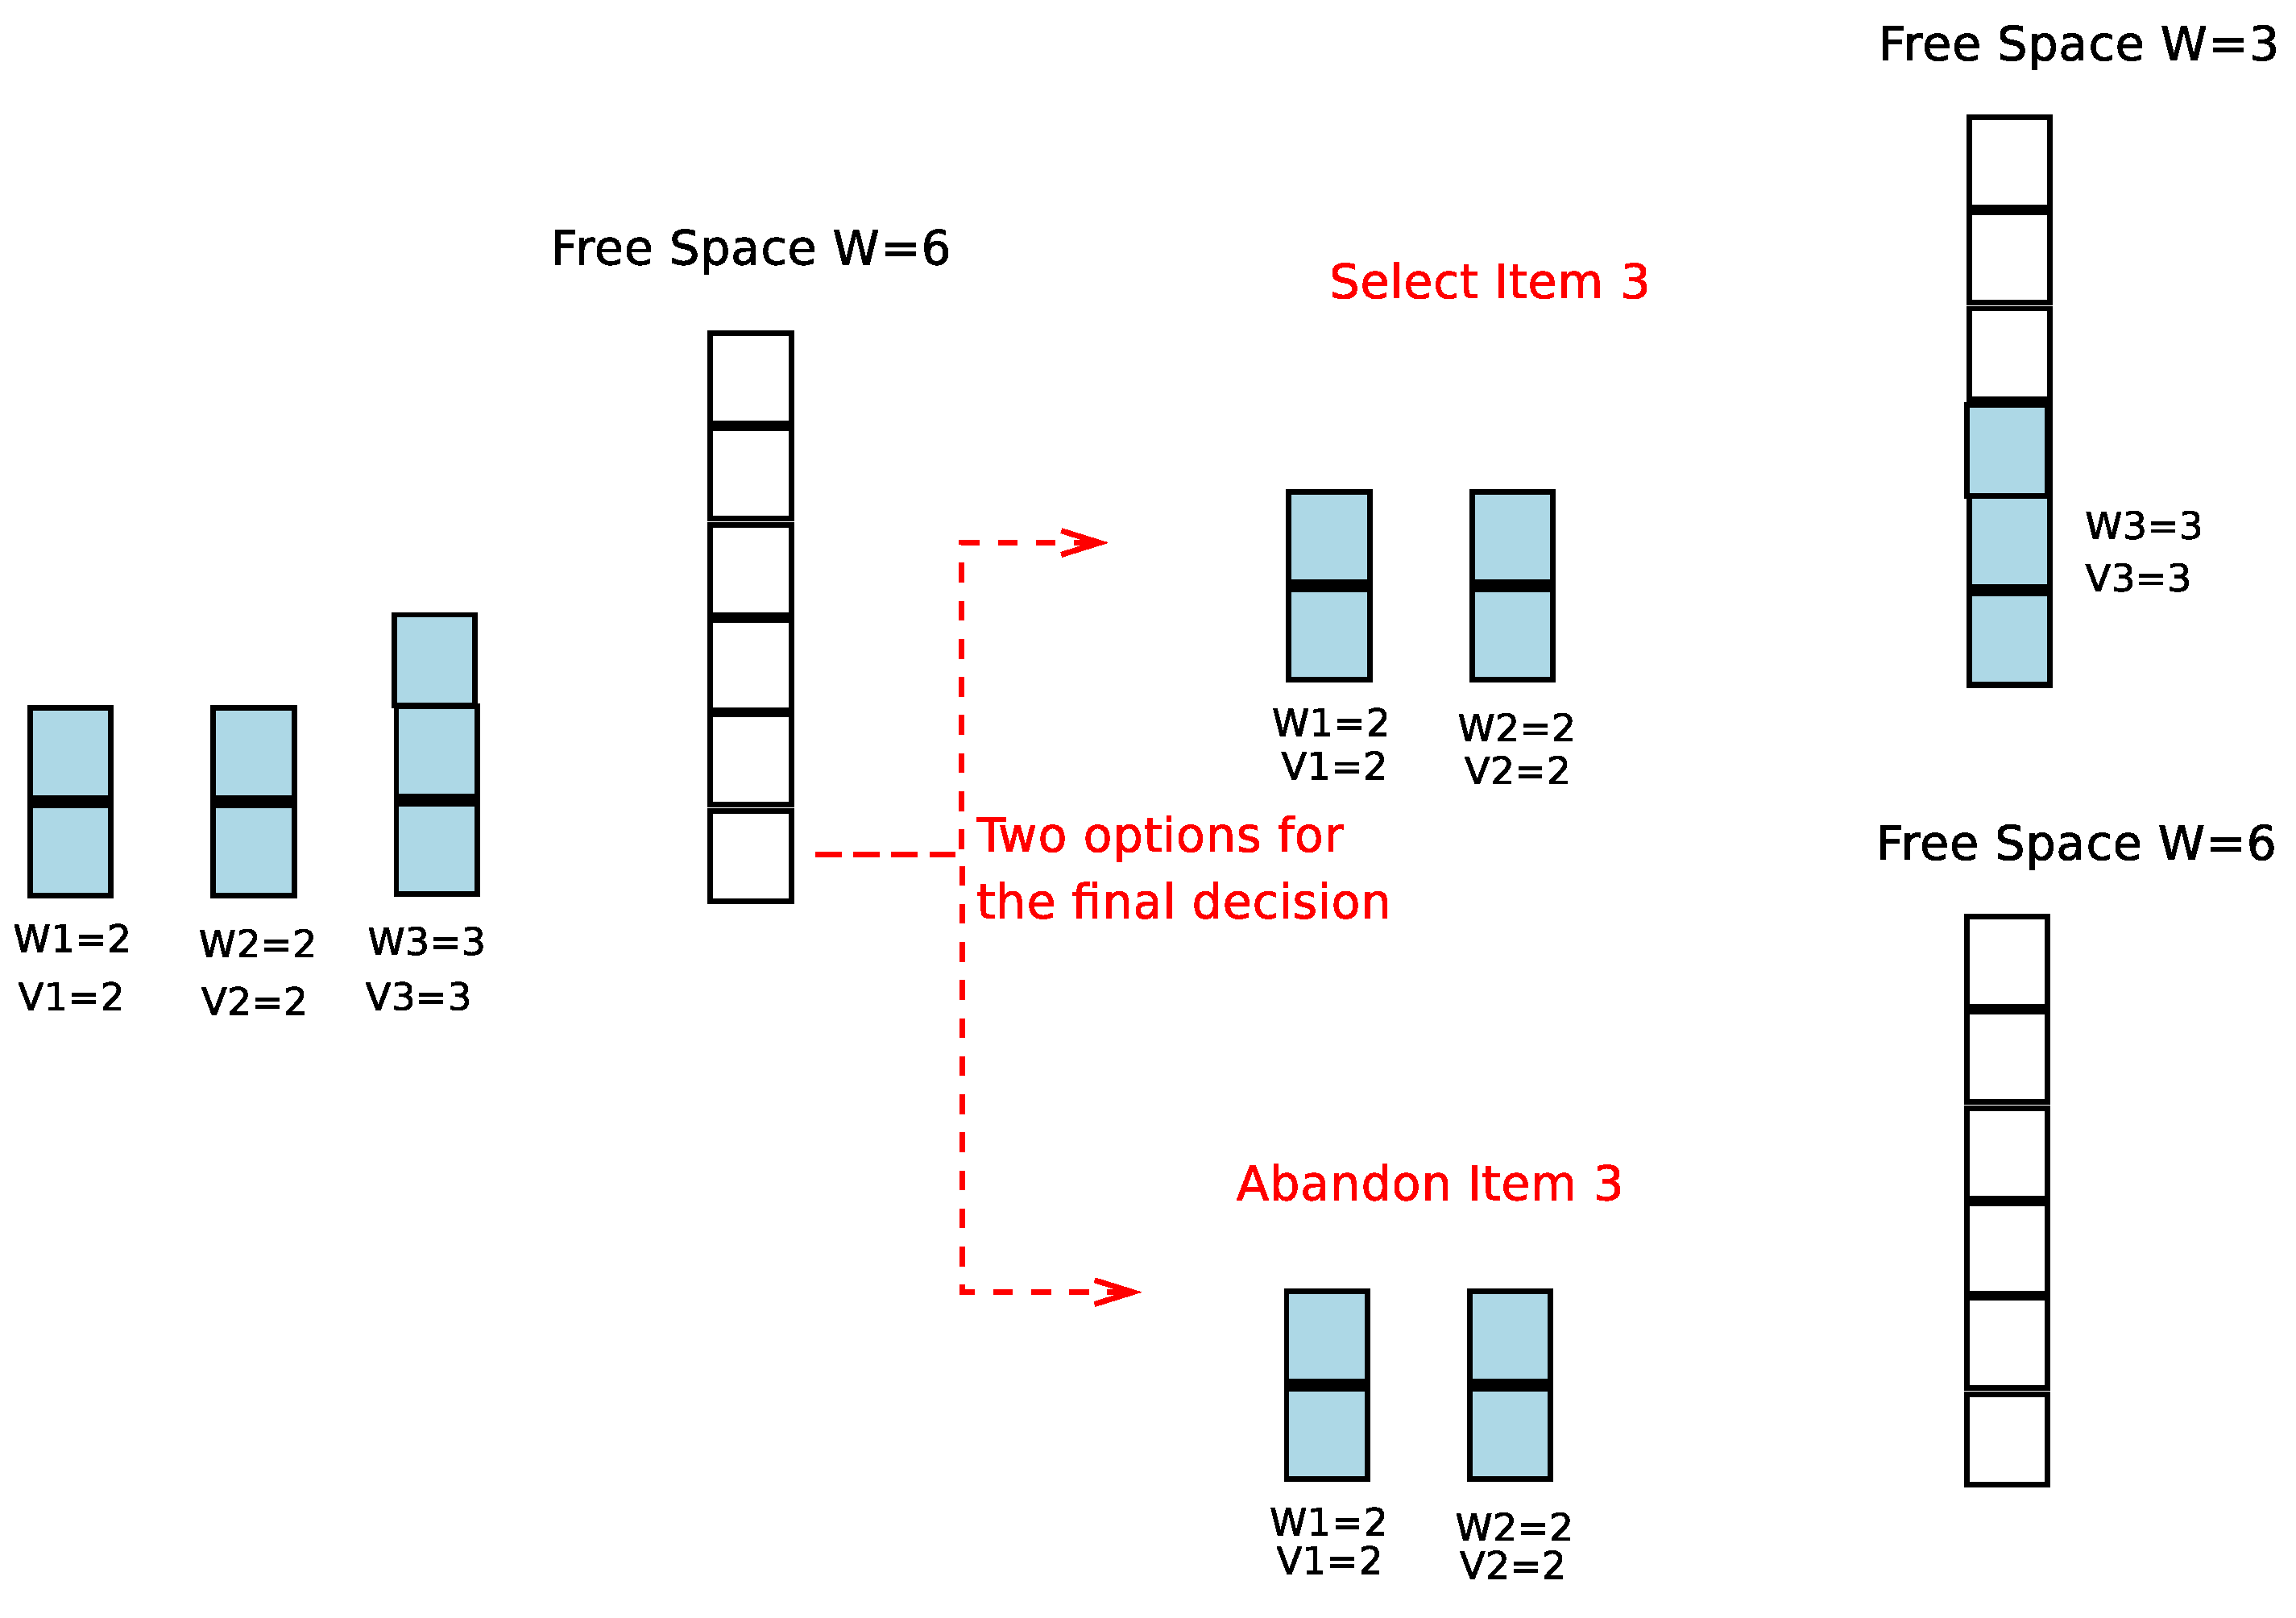
\includegraphics[width=2.3in]{L6-Knapsackexample.eps}
%	\end{figure}
	\end{itemize}

 

} 


\frame{
\frametitle{An example}
\begin{figure}
\begin{tikzpicture}[scale=1., auto,swap]

  \def\dx{0};
  \def\dy{0}; 
  \def\u{0.8};
  
   \foreach \x/\y/\name/\label in {0/0/root/0, 0/-1/L11/1, 1/-1/L12/2, 2/-1/L13/3, 4/-1/L14/4} 
          \node[smallvertex,draw=black, fill=white!20] (\name) at (\x*\u+\dx, \y + \dy) {\tiny $\label$};
  
   \foreach \x/\y/\name/\label in {2/-2/L22/5/, 4/-2/L24/6, 5/-2/L25/7}
          \node[smallvertex,draw=black, fill=yellow] (\name) at (\x*\u+\dx, \y + \dy) {\tiny $\label$};



%   \foreach \x/\y/\name/\label in {1/-1/L12/9, 2/-1/L13/7, 4/-1/L14/5,5/-2/L25/12} 
%          \node[smallvertex,draw=black, fill=yellow] (\name) at (\x*\u+\dx, \y + \dy) {\tiny $\label$};
  

  
  \foreach \source/ \dest /\weight in {root/L11/{}, root/L12/{}, root/L13/{}, root/L14/{}}
         \path[undirectededge] (\source) -- node[weight] {\small $\weight$} (\dest);
 
  \foreach \source/ \dest /\weight in {L13/L22/{},  L14/L24/{}, L14/L25/{}}
         \path[undirectededge] (\source) -- node[weight] {\small $\weight$} (\dest);
 

  \node[above, blue, ultra thick] at (root.north) {$root$};
  
  
   \end{tikzpicture}
\end{figure}

	\begin{itemize}
		\item In both cases, the original problem is reduced into smaller sub-problems.
		\item General form of sub-problems: find minimum vertex cover on a tree rooted at node $v$. Let's denote the optimal solution as $OPT(v)$. 
		\item Thus we have the following recursion: 
\begin{small}
		$OPT(root)  = \min\begin{cases}		
1 + \sum_{c} OPT(c) & c \text{ is a child}  \\
\#children + \sum_{g} OPT(g) & g \text{ is a grand-child} 
                                   \end{cases}$
\end{small}

		\item Time complexity: $O(n)$ (Reason: each node will be visited twice.)
%		In both cases, the original problem is reduced into smaller sub-problems. 
%	\begin{figure}
%	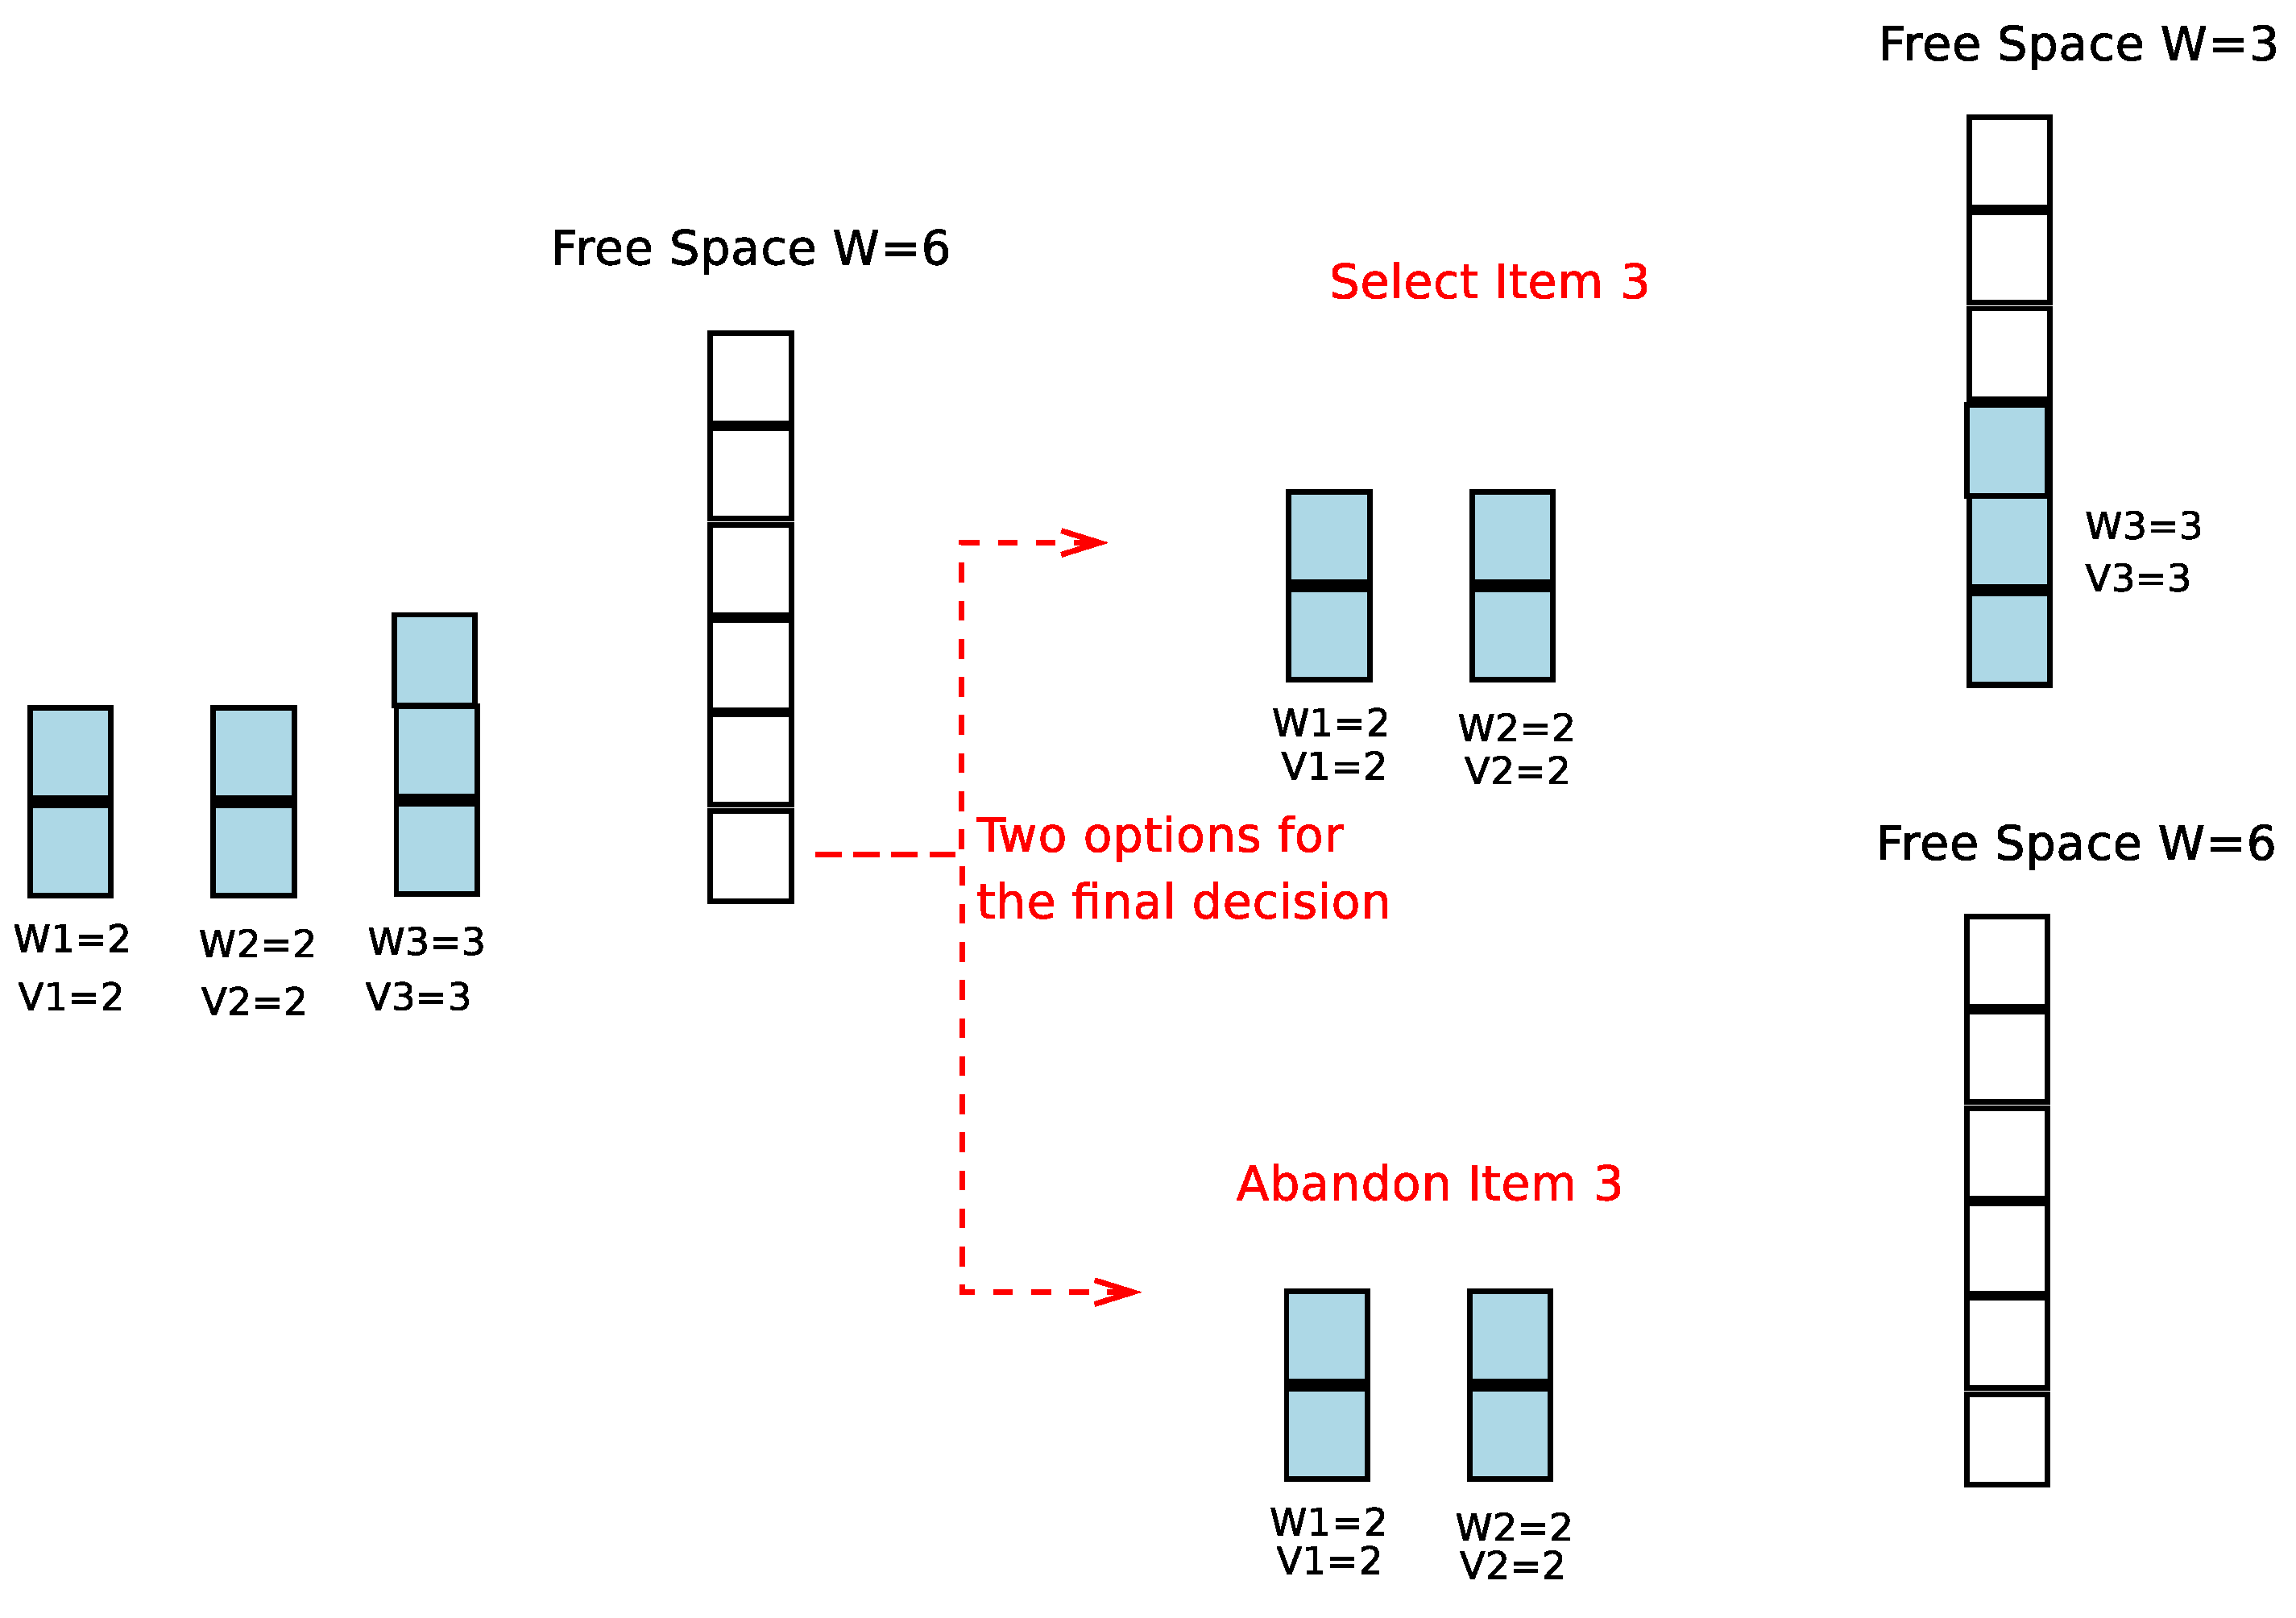
\includegraphics[width=2.3in]{L6-Knapsackexample.eps}
%	\end{figure}
	\end{itemize}

 

} 


\frame{
\begin{block}{}
 {\sc RNA Secondary Structure Prediction}: recursion over \textcolor{red}{\bf sequence} 
\end{block}
}

\frame
{
  \frametitle{RNA secondary structure}
  \begin{itemize}
   \item RNA is a sequence of nucleic acids. It will automatically form structures in water through the formation of bonds $A-U$ and $C-G$. 
\item The native structure is the conformation with the lowest energy. Here, we simply use the number of base pairs as the energy function. 
  \end{itemize}
	\begin{figure}
	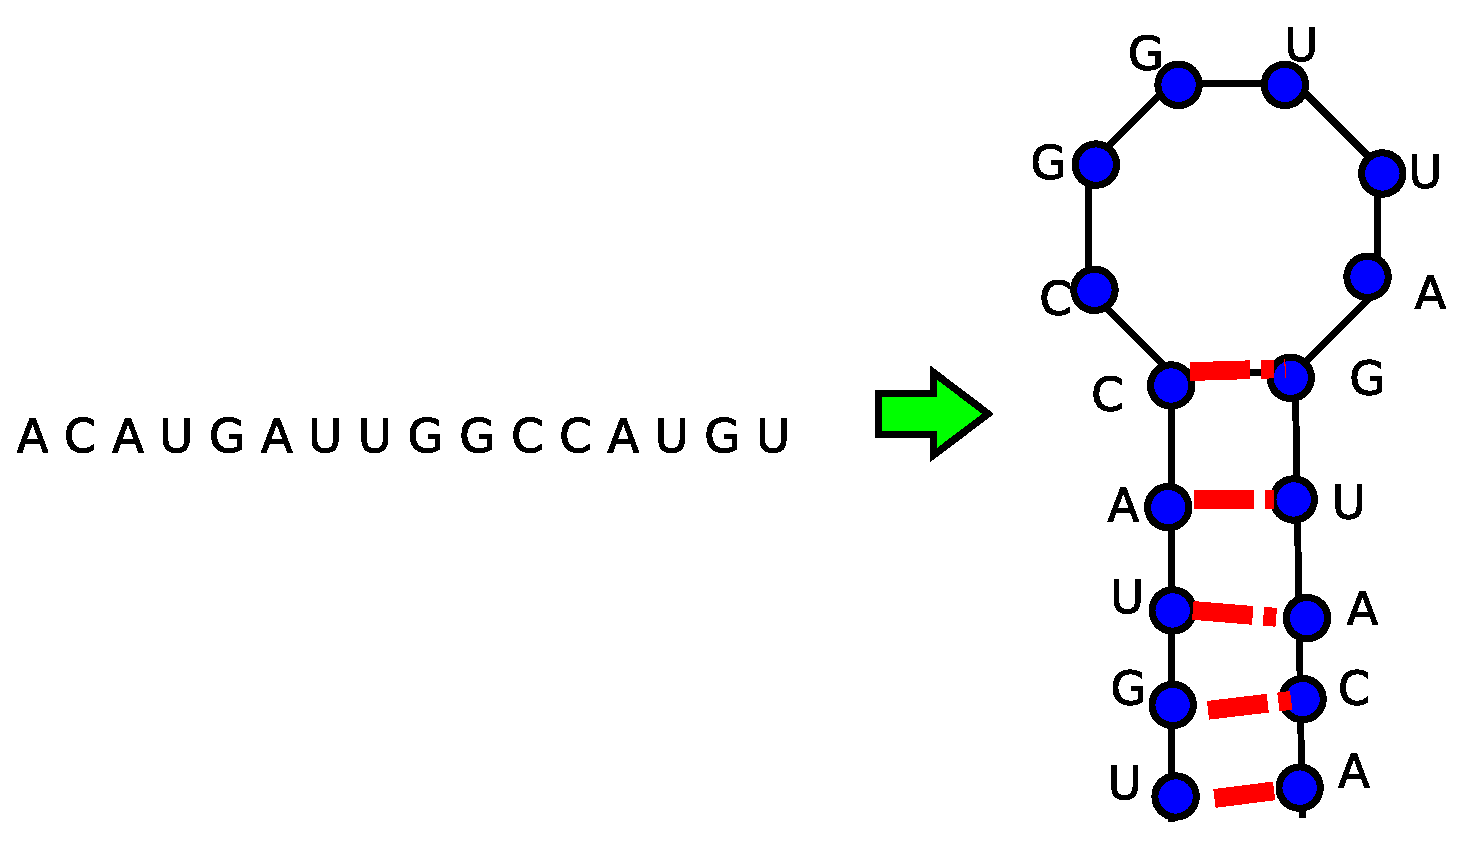
\includegraphics[width=3in]{L6-RNA.eps}
	\end{figure}
}

\frame
{
  \frametitle{Formulation}

\begin{block}{}
{\bf  INPUT: }\\ A sequence in alphabet $\Sigma=\{A, U, C, G\}$;	\\
{\bf OUTPUT: }\\ A pairing scheme with the maximum pairing number
\end{block}

Requirements of base pairs: 
\begin{enumerate}
	 \item Watson-Crick pair: $A$ pairs with $U$, and $C$ pairs with $G$;
 	\item There is no base occurring in more than $1$ base pairs; 
 	\item No cross-over (nesting): there is no crossover under the assumption of free pseudo-knots. 
 	\item And two bases $i, j $ $(|i-j| \leq 4)$ cannot form a base pair. 
\end{enumerate}

}

%\frame{
%\frametitle{An example}
%	\begin{figure}
%	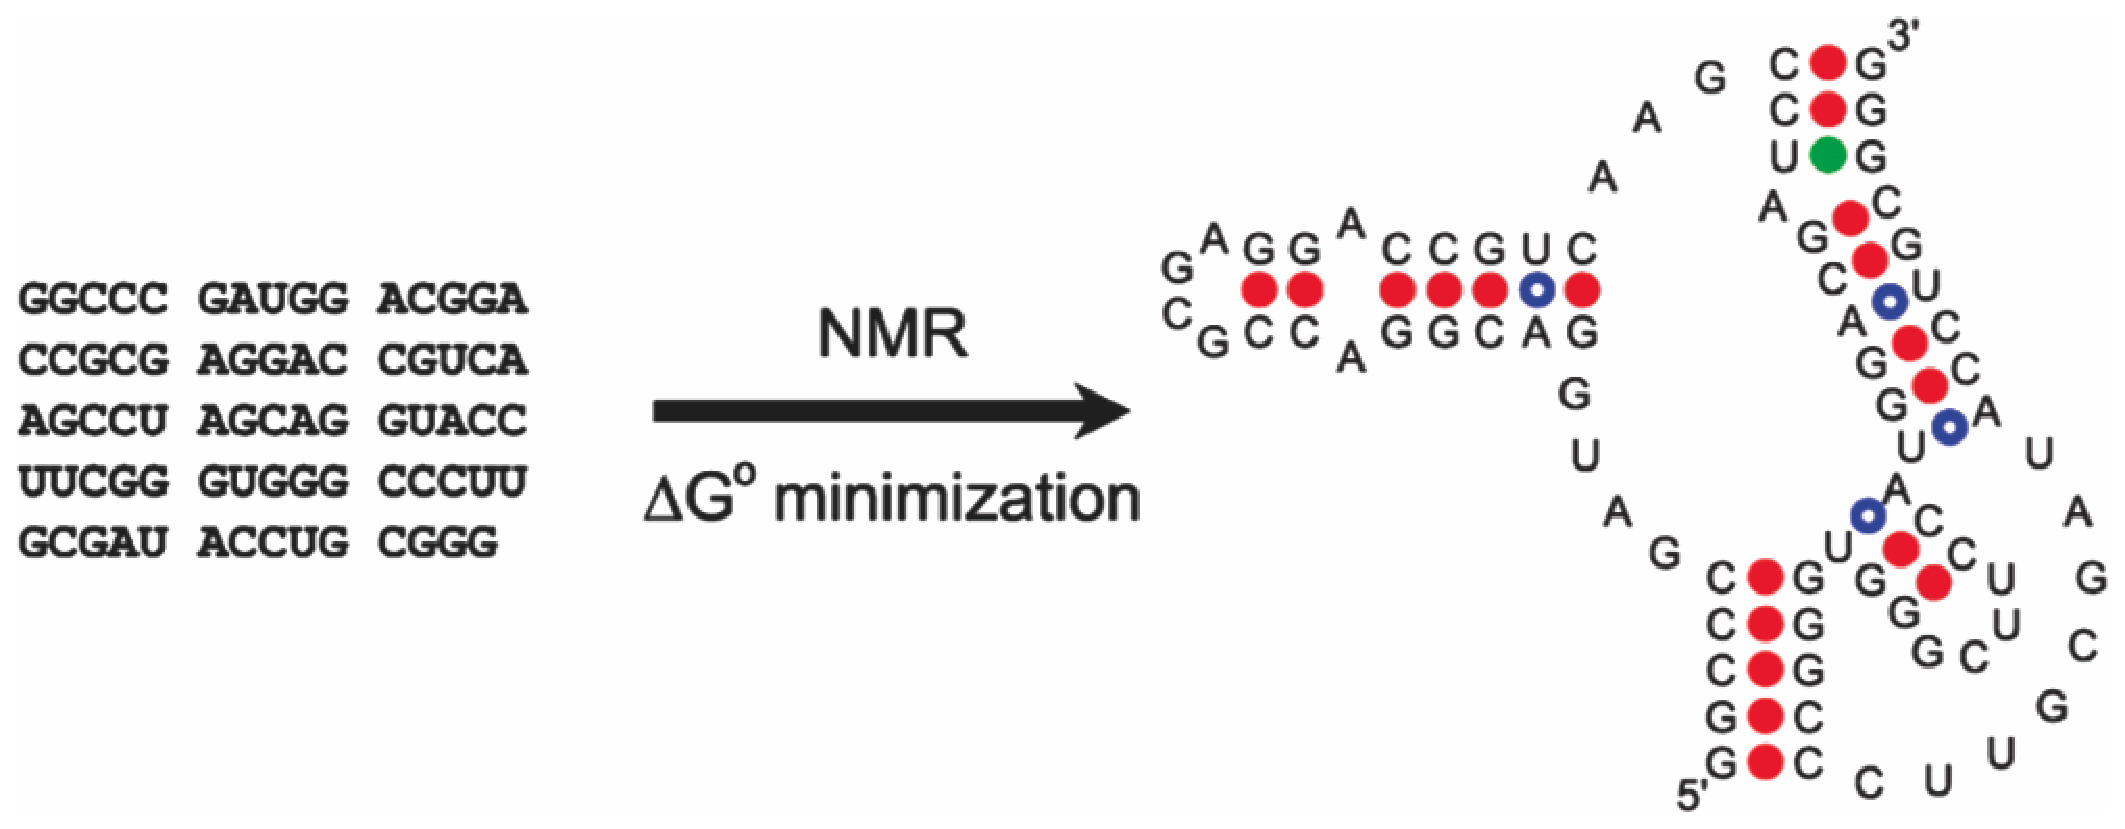
\includegraphics[width=4in]{L6-RNA-2D.eps}
%	\end{figure}
%}


\frame{
\frametitle{Nesting and Pseudo-knot}

\begin{figure}[H]\centering
\begin{tikzpicture}[scale=0.8, auto,swap]
 
 
    \def\dx{0};
    \def\dy{0};
%    \foreach \x/\y/\letter in { 0/0/G/R0,  1/0/U/R1, 2/0/G/R1, 3/0/A/R1, 4/0/U/R1, 5/0/C/R1, 6/0/U/R1, 7/0/G/R1, 8/0/G, 9/0/A, 10/0/C, 11/0/U, 12/0/A, 13/0/G, 14/0/A, 15/0/C, 16/0/A, 17/0/G, 18/0/A, 19/0/U, 20/0/C, 21/0/C, 22/0/U }

    \foreach \x/\y/\letter in { 0/0/G,  1/0/U, 2/0/G, 3/0/A, 4/0/U, 5/0/C, 6/0/U, 7/0/G, 8/0/G, 9/0/A, 10/0/C, 11/0/U, 12/0/A, 13/0/G, 14/0/A, 15/0/C, 16/0/A, 17/0/G, 18/0/A, 19/0/U, 20/0/C, 21/0/C, 22/0/U }
        \node[smallvertex, fill=blue!20] (R\x) at (\x*0.6+\dx, \y+\dy) {\small {\tt \letter}};
        
        
    \foreach \source/\dest/\weight in {R0/R1/, R1/R2/, R2/R3/, R3/R4/, R4/R5/, R5/R6/, R6/R7/, R7/R8/, R8/R9/, R9/R10/, R10/R11/, R11/R12/, R12/R13/, R13/R14/, R14/R15/, R15/R16/, R16/R17/, R17/R18/, R18/R19/, R19/R20/, R20/R21/, R21/R22/  } 
            \path[undirectededge] (\source) -- node{\small $\weight$} (\dest);

    \draw[-, thick, blue] (R1) to[out=30, in=150]  (R9);
    \draw[-, thick, blue] (R12) to[out=30, in=150]  (R22);
    \draw[-, thick, blue] (R13) to[out=30, in=150]  (R21);
    \node[below] at (R11.south) {$(a)$}; 		
				
 
    \def\dx{0};
    \def\dy{-2.};
%    \foreach \x/\y/\letter in { 0/0/G/R0,  1/0/U/R1, 2/0/G/R1, 3/0/A/R1, 4/0/U/R1, 5/0/C/R1, 6/0/U/R1, 7/0/G/R1, 8/0/G, 9/0/A, 10/0/C, 11/0/U, 12/0/A, 13/0/G, 14/0/A, 15/0/C, 16/0/A, 17/0/G, 18/0/A, 19/0/U, 20/0/C, 21/0/C, 22/0/U }

    \foreach \x/\y/\letter in { 0/0/G,  1/0/U, 2/0/G, 3/0/A, 4/0/U, 5/0/C, 6/0/U, 7/0/G, 8/0/G, 9/0/A, 10/0/C, 11/0/U, 12/0/A, 13/0/G, 14/0/A, 15/0/C, 16/0/A, 17/0/G, 18/0/A, 19/0/U, 20/0/C, 21/0/C, 22/0/U }
        \node[smallvertex, fill=blue!20] (R\x) at (\x*0.6+\dx, \y+\dy) {\small {\tt \letter}};
        
        
    \foreach \source/\dest/\weight in {R0/R1/, R1/R2/, R2/R3/, R3/R4/, R4/R5/, R5/R6/, R6/R7/, R7/R8/, R8/R9/, R9/R10/, R10/R11/, R11/R12/, R12/R13/, R13/R14/, R14/R15/, R15/R16/, R16/R17/, R17/R18/, R18/R19/, R19/R20/, R20/R21/, R21/R22/  } 
            \path[undirectededge] (\source) -- node{\small $\weight$} (\dest);

    \draw[-, thick, red] (R1) to[out=30, in=150]  (R9);
    \draw[-, thick, red] (R5) to[out=30, in=150]  (R13);

    \node[below] at (R11.south) {$(b)$}; 		
				

		
\end{tikzpicture} 
\label{PseudoKnot}
\caption{ Two base pairs should be independent of nested $(a)$ but cannot form cross-over ($b$).}

\end{figure}    

}

%\frame{
%\frametitle{Feymann graph }
%\begin{figure}%
% 	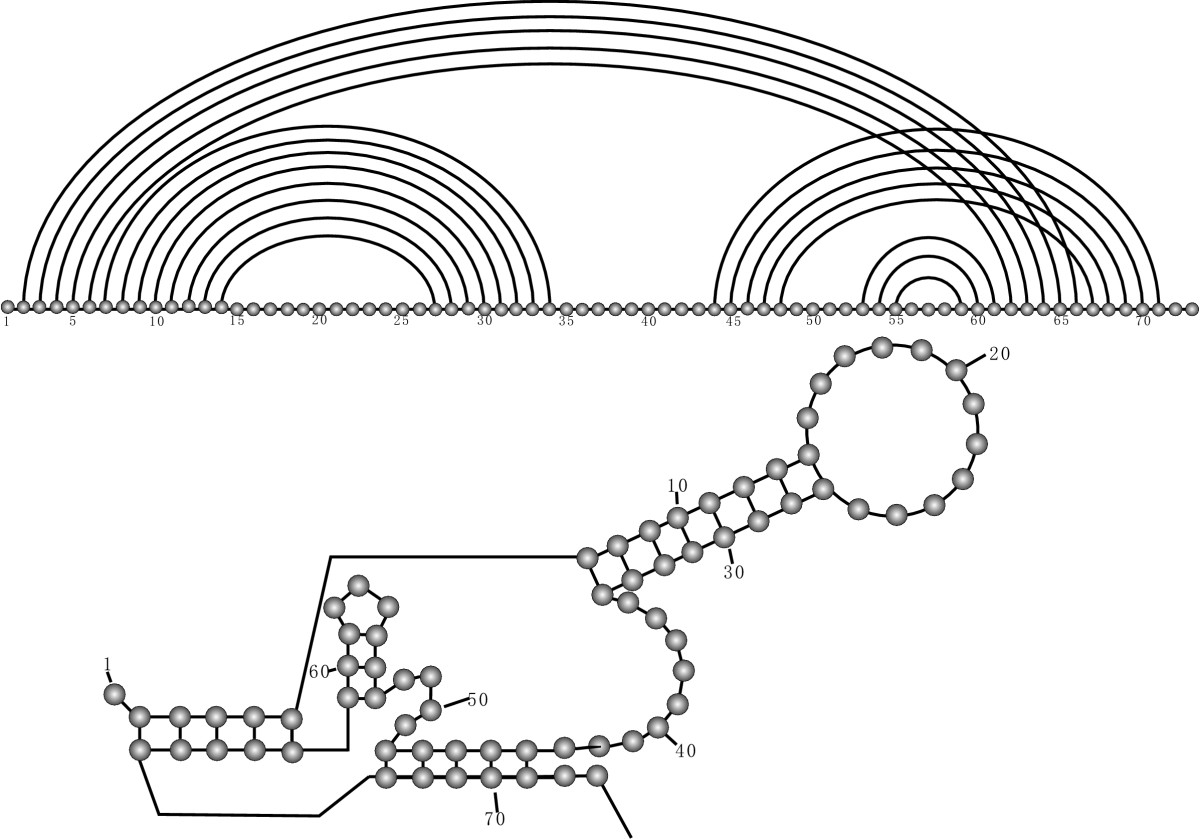
\includegraphics[width=3.0in]{L6-RNA-Feymann.png}
%\end{figure}
%Feymann graph: an intuitive representation form of RNA secondary structure, i.e.  two bases are connected by an edge if they form a Watson-Crick pair.
%} 

\frame{
\frametitle{Defining general form of sub-problems}
\begin{itemize}
 	\item Solution: a set of \textcolor{red}{nested} base pairs. Describe the solving process as as  a process of multistage \textcolor{red}{\bf decisions}. At the $i$-th decision stage, we determine whether base $i$ forms pair or not. 
%  	\item Suppose we have already worked out the optimal solution. 
 	\item Let's consider the $first$ decision made for base $n$ in the optimal solution. There are two options: 
 \begin{enumerate}
  	\item Base $n$ pairs with a base $i$: we should calculate optimal pairs for regions $i+1..n-1$ and $1..i-1$.  Note that these two sub-problems are independent due to the ``nested'' property. 
  	\item Base $n$ doesn't form a pair: we should calculate optimal pairs for regions $1..n-1$. 
 \end{enumerate}
	\item Thus we can design the general form of sub-problems as: to calculate the optimal pairs for region $i..j$. (Denote the optimal solution value as: $OPT(i,j)$.)
\end{itemize}

 }
 
 \frame{
 	\frametitle{Optimal sub-structure property}  

\begin{figure}[H]\centering
\begin{tikzpicture}[scale=0.8, auto,swap]
 
 
    \def\dx{0};
    \def\dy{0};
    \def\scale{0.6};
%    \foreach \x/\y/\letter in { 0/0/G/R0,  1/0/U/R1, 2/0/G/R1, 3/0/A/R1, 4/0/U/R1, 5/0/C/R1, 6/0/U/R1, 7/0/G/R1, 8/0/G, 9/0/A, 10/0/C, 11/0/U, 12/0/A, 13/0/G, 14/0/A, 15/0/C, 16/0/A, 17/0/G, 18/0/A, 19/0/U, 20/0/C, 21/0/C, 22/0/U }

    \foreach \x/\y/\letter in { 0/0/G,  1/0/U, 2/0/G, 3/0/A, 4/0/U, 5/0/C, 6/0/U, 7/0/G, 8/0/G, 9/0/A, 10/0/C, 11/0/U, 12/0/A, 13/0/G, 14/0/A, 15/0/C, 16/0/A, 17/0/G, 18/0/A, 19/0/U, 20/0/C, 21/0/C, 22/0/U }
        \node[smallvertex, fill=blue!20] (R\x) at (\x*0.6+\dx, \y+\dy) {\small {\tt \letter}};
        
        
    \foreach \source/\dest/\weight in {R0/R1/, R1/R2/, R2/R3/, R3/R4/, R4/R5/, R5/R6/, R6/R7/, R7/R8/, R8/R9/, R9/R10/, R10/R11/, R11/R12/, R12/R13/, R13/R14/, R14/R15/, R15/R16/, R16/R17/, R17/R18/, R18/R19/, R19/R20/, R20/R21/, R21/R22/  } 
            \path[undirectededge] (\source) -- node{\small $\weight$} (\dest);

%    \draw[-, thick, blue] (R1) to[out=30, in=150]  (R9);
%    \draw[-, thick, blue] (R12) to[out=30, in=150]  (R22);
%    \draw[-, thick, blue] (R13) to[out=30, in=150]  (R21);
    \node[below] at (R22.south) {$R_n$};
    \draw[thick, red] ( 0 * \scale + \dx - 0.25, 0 + \dy + 0.25 ) rectangle ( 21 * \scale + \dx + 0.25, 0 + \dy - 0.25); 		
  
    \node[below] at (R11.south) {$(a)$}; 		
				
 
    \def\dx{0};
    \def\dy{-2.};
%    \foreach \x/\y/\letter in { 0/0/G/R0,  1/0/U/R1, 2/0/G/R1, 3/0/A/R1, 4/0/U/R1, 5/0/C/R1, 6/0/U/R1, 7/0/G/R1, 8/0/G, 9/0/A, 10/0/C, 11/0/U, 12/0/A, 13/0/G, 14/0/A, 15/0/C, 16/0/A, 17/0/G, 18/0/A, 19/0/U, 20/0/C, 21/0/C, 22/0/U }

    \foreach \x/\y/\letter in { 0/0/G,  1/0/U, 2/0/G, 3/0/A, 4/0/U, 5/0/C, 6/0/U, 7/0/G, 8/0/G, 9/0/A, 10/0/C, 11/0/U, 12/0/A, 13/0/G, 14/0/A, 15/0/C, 16/0/A, 17/0/G, 18/0/A, 19/0/U, 20/0/C, 21/0/C, 22/0/U }
        \node[smallvertex, fill=blue!20] (R\x) at (\x*0.6+\dx, \y+\dy) {\small {\tt \letter}};
        
        
    \foreach \source/\dest/\weight in {R0/R1/, R1/R2/, R2/R3/, R3/R4/, R4/R5/, R5/R6/, R6/R7/, R7/R8/, R8/R9/, R9/R10/, R10/R11/, R11/R12/, R12/R13/, R13/R14/, R14/R15/, R15/R16/, R16/R17/, R17/R18/, R18/R19/, R19/R20/, R20/R21/, R21/R22/  } 
            \path[undirectededge] (\source) -- node{\small $\weight$} (\dest);

    \draw[-, thick, blue] (R12) to[out=30, in=150]  (R22);
    \draw[thick, red] ( 0  * \scale + \dx - 0.25, 0 + \dy + 0.25 ) rectangle ( 11  * \scale + \dx + 0.25, 0 + \dy - 0.25); 
    \draw[thick, red] ( 13  * \scale + \dx - 0.25, 0 + \dy + 0.25 ) rectangle ( 21  * \scale + \dx + 0.25, 0 + \dy - 0.25); 		
    \node[below] at (R12.south) {$R_{k}$};
    \node[below] at (R22.south) {$R_n$};
    
    \node[below] at (R11.south) {$(b)$}; 		
				

		
\end{tikzpicture} 
\label{RNAFold2Options}
%\caption{\fangsong 多步决策过程中第一步决策的两个选择项:$(a)$ 碱基$R_n$不和任何碱基配对;$(b)$ 碱基$R_n$与碱基$R_i$配对。}

\end{figure}    
	
\begin{itemize}
 	\item Optimal substructures property: 
$OPT(1,n) = \max \begin{cases} OPT(1, n-1) & \\ 
 \max\limits_{\substack{1 \leq k < n-4\\ R_k \text{ pairs with } R_n}}\{1 + OPT( 1, k-1) + OPT( k+1, n-1) \} \} & 
 \end{cases}$. 
\end{itemize}
}

\frame{
\frametitle{Algorithm}
{\sc RNA2D}$( n )$
\begin{algorithmic}[1]
\STATE Initialize all $OPT[i,j]$ with $0$;
\FOR{$i=1$ to $n$ }
	\FOR{$j=i+5$ to $n$ }
		\STATE $OPT[i, j] = \max\{OPT[i,j-1], \max_{t} \{1+OPT[i,t-1]+OPT[t+1,j-1] \} \}$;
		\STATE /* $t$ and $j$ can form Watson-Crick base pair. */
	\ENDFOR
\ENDFOR
\end{algorithmic}
}


\frame{
	\frametitle{An example}
	
	\begin{table}[H]\centering
%\caption{ {\sc RNA2D}算法运行过程示例。}
\label{IterativeRNA2DExample}
 % \begin{minipage}[c]{0.45\linewidth}
 % 	\caption{OPT}
    \centering
%    %\begin{table}[!ht]
%      \centering
      \begin{tabular}{c|c|c|c|c| c|c|c|c|c| c|c|c|c|c| c|c|c|c|c| }
        \multicolumn{1}{r}{$j=$}& \multicolumn{1}{c}{6} & \multicolumn{1}{c}{7} & \multicolumn{1}{c}{8} & \multicolumn{1}{c}{9}&  \multicolumn{1}{r}{ } &   \multicolumn{1}{c}{6} & \multicolumn{1}{c}{7} & \multicolumn{1}{c}{8} & \multicolumn{1}{c}{9}&  \multicolumn{1}{r}{ } &  \multicolumn{1}{c}{6} & \multicolumn{1}{c}{7} & \multicolumn{1}{c}{8} & \multicolumn{1}{c}{9}&   \multicolumn{1}{r}{ }& \multicolumn{1}{c}{6} & \multicolumn{1}{c}{7} & \multicolumn{1}{c}{8} & \multicolumn{1}{c}{9}  \\
        \hhline{~----~----~----~----}
        $i=4$ & 0 & 0 & 0 & 0  &   & 0 & 0 & 0 & 0  &  & 0 & 0 & 0 & 0  &  & 0 & 0 & 0 & 0     \\
        \hhline{~----~----~----~----}
        $i=3$ & 0 & 0 & 1 &    &   & 0 & 0 & 1 & 1   &  & 0 & 0 & 1 & 1  &  & 0 & 0 & 1 & 1      \\
        \hhline{~----~----~----~----}
        $i=2$ & 0 & 0 &   &    &   & 0 & 0 & 1 &       &  & 0 & 0 & 1 & 1  &  & 0 & 0 & 1 & 1     \\
        \hhline{~----~----~----~----}
        $i=1$ & 1 &   &   &   &   & 1 & 1 &   &         &  & 1 & 1 & 1 &      &  & 1 & 1 & 1 & 2     \\
        \hhline{~----~----~----~----} 
       \multicolumn{1}{c}{ } & \multicolumn{4}{c}{$ (a)$}&    \multicolumn{1}{c}{ } & \multicolumn{4}{c}{$ (b)$}&   \multicolumn{1}{c}{ } & \multicolumn{4}{c}{$ (c)$}&   \multicolumn{1}{c}{ } & \multicolumn{4}{c}{$ (d)$} 
      \end{tabular}
\end{table}


\begin{figure}[H]\centering
\begin{tikzpicture}[scale=1.0, auto,swap]
 
 
    \def\dx{0};
    \def\dy{0};
    \def\scale{0.6};



    \foreach \x/\y/\letter in { 0/0/A,  1/0/C, 2/0/C, 3/0/G, 4/0/G, 5/0/U, 6/0/A, 7/0/G, 8/0/U }
        \node[smallvertex, fill=blue!20] (R\x) at (\x*0.6+\dx, \y+\dy) {\small {\tt \letter}};
        
        
    \foreach \source/\dest/\weight in {R0/R1/, R1/R2/, R2/R3/, R3/R4/, R4/R5/, R5/R6/, R6/R7/, R7/R8/ } 
            \path[undirectededge] (\source) -- node{\small $\weight$} (\dest);

    \draw[-, thick, blue] (R0) to[out=30, in=150]  (R8);
    \draw[-, thick, blue] (R1) to[out=30, in=150]  (R7);
    				
\end{tikzpicture} 
\label{RNA2DResult}
%\caption{\fangsong 算法{\sc RNA2D}对RNA序列{\tt ACCGGUAGU}预测出的二级结构。}

\end{figure}    



%		\begin{figure}
%			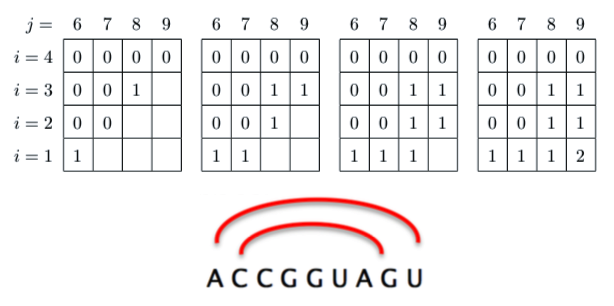
\includegraphics[width=3.5in]{L6-RNAFolding.png}
%		\end{figure}
Time complexity: $O(n^3)$. 
}

%\frame{
%	\frametitle{Step 2}
%
%\begin{figure}
%	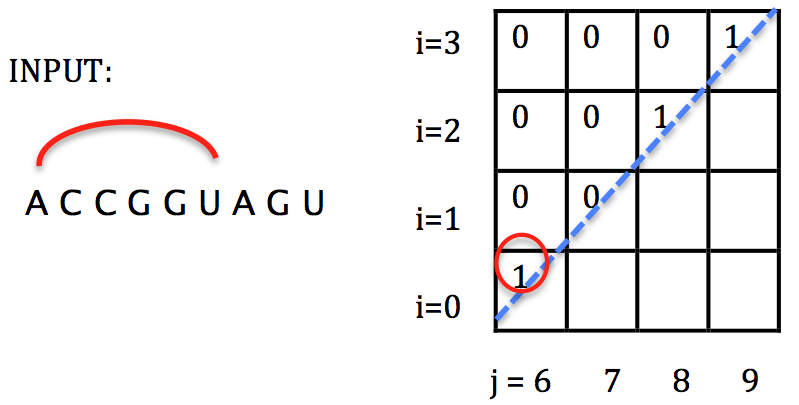
\includegraphics[width=3.5in]{L6-RNAalgostep2.png}
%	\end{figure}
%}
%	
%\frame{
%	\frametitle{Step 3}
%	
%\begin{figure}
%	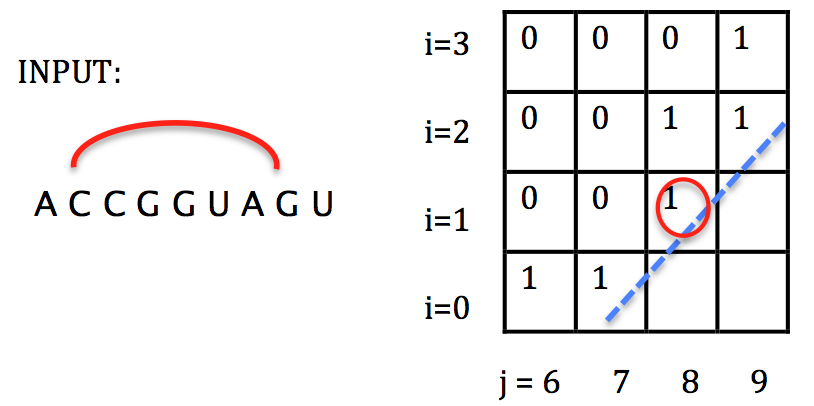
\includegraphics[width=3.5in]{L6-RNAalgostep3.png}
%	\end{figure}
%}
%
%\frame{
%	\frametitle{Step 4}
%	
%\begin{figure}
%	\includegraphics[width=3.5in]{L6-RNAalgostep1-4.png}
%\end{figure}
%Time complexity: $O(n^3)$. 
%}

\frame{
  \frametitle{Extension: RNA is a good example of SCFG.}

  \begin{figure}
  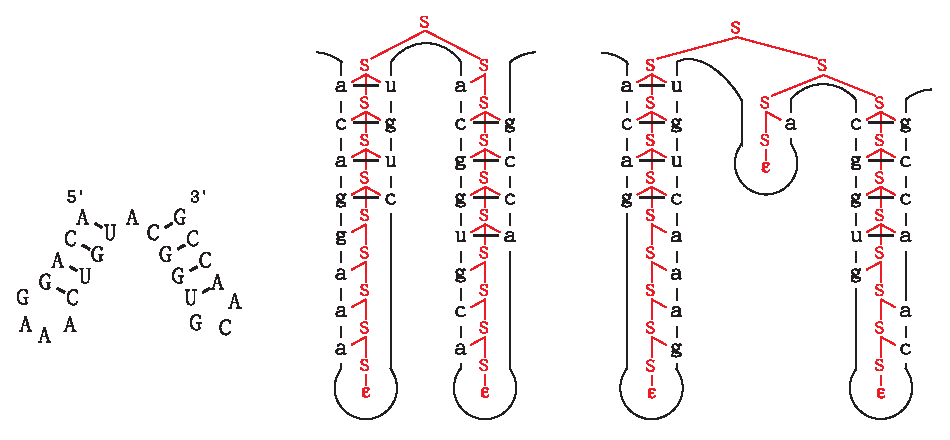
\includegraphics[width=3in]{SCFG.eps}
  \end{figure}

(see extra slides)
}

% \frame[allowframebreaks]
% {
% \frametitle{Sequence Alignment}
% 	\begin{block}{Description}
% 	{\bf Input: } 2 sequences $S_1$ and $S_2$\\
% 	{\bf Output: } a mapping from $S_1$ to $S_2$ allowing \emph{insert} and \emph{delete} to make the \emph{scoring function} smallest.
% 	\end{block}
% 
% 	\begin{block}{Example}
% 		\begin{center}
% 			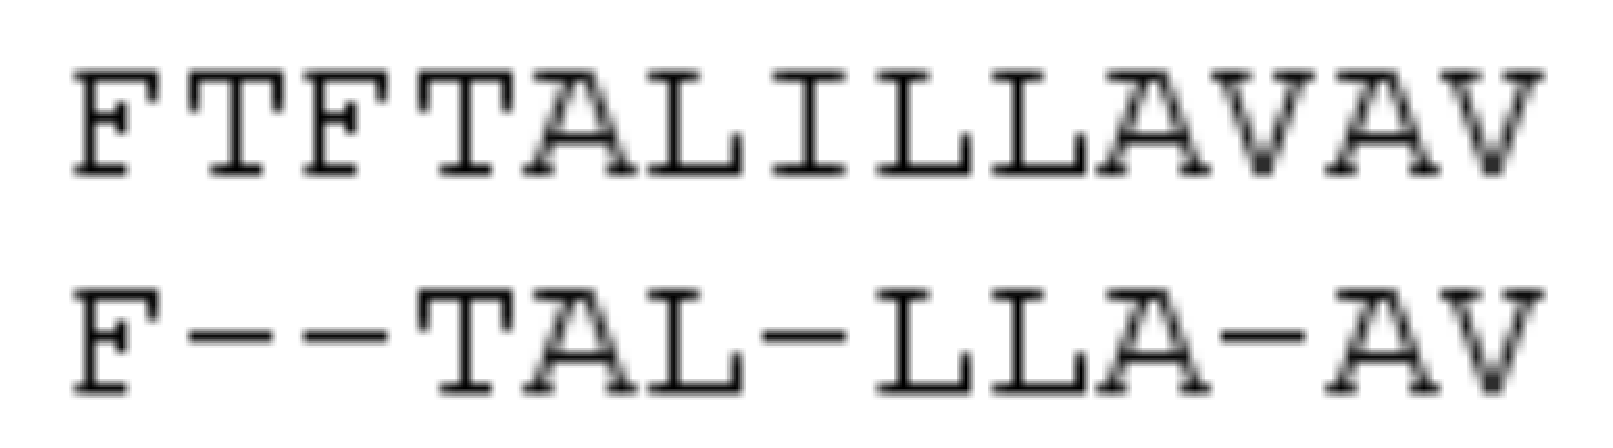
\includegraphics[width=0.5\textwidth]{p51.eps}
% 		\end{center}
% 		\begin{center}
% 			
\includegraphics[width=0.5\textwidth]{p52.eps}
% 		\end{center}
% 
% 	\end{block}
% 
% }
 

\frame{
\begin{block}{}
 {\sc Sequence Alignment}  problem: recursion over \textcolor{red}{\bf sequence pairs}
\end{block}
}

\frame{
\frametitle{Practical  problem: genome similarity  }



\begin{small}
\begin{itemize}
\begin{small}
	\item To identify homology genes of two species, say $Human$ and $Mouse$. Human and Mouse NHPPEs (in KRAS genes) show a high sequence homology (Ref: Cogoi, S., et al. NAR, 2006).  

%\begin{figure}
%\begin{tikzpicture}[scale=0.8, auto,swap]
%	\node at (0, 0) {\texttt{GGGCGGTGTGGGAA-GAGGGAAG-AGGGGGAG}}; 
%	\node at (0, -0.5) {\texttt{|||\ ||\ |\ |||||\ ||||||\ |\ ||||\ |\ \ }}; 
%	\node at (0, -1) {\texttt{GGGAGG-GAGGGAAGGAGGGAGGGAGGGAG--}};
%\end{tikzpicture}
%\end{figure}

\begin{figure}
\begin{tikzpicture}[scale=0.8, auto,swap]
	\node at (0, 0) {\texttt{GGGCGGTGTG}}; 
	\node at (0, -0.5) {\texttt{|||\ ||\ |\ |}}; 
	\node at (0, -1) {\texttt{GGGAGG-GAG}};
\end{tikzpicture}
\end{figure}

	\item Having calculating the similarity of genomes of various species, a reasonable phylogeny tree can be estimated (See https://www.llnl.gov/str/June05/Ovcharenko.html)

\begin{figure}
	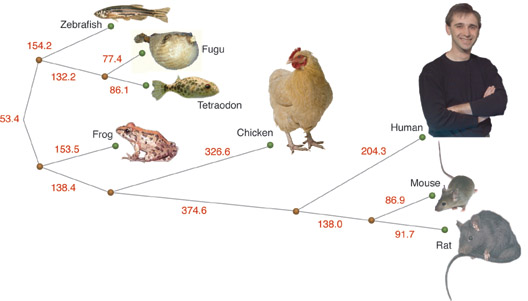
\includegraphics[width=2.9in]{L6-phylogenytree.png}
\end{figure}
\end{small}
\end{itemize}
\end{small}
}


\frame{
\frametitle{Practical problem: spell tool to correct typos}

\begin{itemize}
\item 
When you type in "{\tt OCURRANCE}'', spell tools might guess what you really want to type through the following alignment: 
\begin{figure}
\begin{tikzpicture}[scale=0.8, auto,swap]
	\node at (0, 0) {\texttt{O-CURRANCE}}; 
	\node at (0, -0.5) {\texttt{|\ ||||\ |||}}; 
	\node at (0, -1) {\texttt{OCCURRENCE}};
\end{tikzpicture}
\end{figure}
Here,  `\texttt{|}' represent identical characters. 
\item This alignment suggests that "{\tt OCURRANCE}'' is very similar to "{\tt OCCURRENCE}'', i.e., "{\tt OCURRANCE}'' is generated from  "{\tt OCCURRENCE}'' using several  {\tt INS/DEL/MUTATION} operations. 



%\begin{itemize}
% \item \texttt{O-CURRANCE}
%\item \texttt{OCCURRENCE}
%\end{itemize}

%\item 
%But the following instance is a bit difficult:
%
%\begin{itemize}
%\item 
%\texttt{abbbaa-bbbbaab}
%\item 
%\texttt{ababaaabbbba-b}
%\end{itemize}

\end{itemize}
}




\frame{
\frametitle{What is an alignment? } 

\begin{itemize}

\item Alignment is introduced to describe the generating process of  an erroneous word from the correct word  using a series of {\tt Insertion/Deletion/Match/Mutation} operations. 

%For example, the generating of "{\tt OCURRENCE}'' from "{\tt OCCURRANCE}'' can be described as the following alignment: 
%
%Here,  `\texttt{|}' represent identical characters. 

 \item For this aim, we make the two sequences to have the same length through adding space '-' at appropriate positions, which changes $S$ to $S'$, and changes  $T$ to $T'$ with identical length $|S'| = |T'|$. 
\begin{figure}	
\begin{tikzpicture}[scale=0.8, auto,swap]
	\node at (0, 0) {\texttt{S': O-CURR-ANCE}}; 
	\node at (0, -0.5) {\texttt{\ \ \ \ |\ ||||\ \ |||}}; 
	\node at (0, -1) {\texttt{T': OCCURRE-NCE}};
\end{tikzpicture}
\end{figure}
  \item The generating process of $S$ from $T$ is described using spaces '-': 
%  The spaces '-' are introduced to describe .  There are three cases of aligned characters: 
 \begin{enumerate}
	\item $S'[i]=$'-':  $S'[i]$ represents a {\tt deletion} of $T'[i]$. 
 	\item $T'[i]=$'-':  $S'[i]$ represents an inserted letter. % through inserting an extra letter.%{\tt INSERTION}. 
	\item Otherwise, $S'[i]$ is a copy of $T'[i]$ (with possible {\tt mutation}). 
\end{enumerate}
\end{itemize}
}

\frame{
\frametitle{Measuring the possibility of each generating process} 
\begin{itemize}
	\item For each generating process, we can measure its possibility using a linear function: 
\[
s(T,S)=\sum_{i=1}^{|S'|} s( T'[i], S'[i] ) 
\]

	\item Here we assume a simple setting  of $s(a,b)$ as follows:  
	\begin{enumerate}
 		\item {\sc Match}: +1, e.g.  $s$('C', 'C')$ = 1$.\\ 
 		\item {\sc Mutation}: -1, e.g.  $s$('E', 'A') $= -1$.\\
 		\item {\sc Insertion/Deletion}: -3, e.g.  $s$('C', '-')$ = -3$.\\
	\end{enumerate}
\footnote{Ideally, the score function is designed such that $s(T,S)$ is proportional to $\log \Pr[ S\text{ is generated from } T]$. See extra slides for the statistical model for sequence alignment, and better similarity definition, say BLOSUM62, PAM250 substitution matrix, etc.}
\end{itemize}
}

\frame{
\frametitle{Alignment is useful   }

\begin{itemize}
\item Application 1: Using alignment, we can determine the most likely source of "{\tt OCURRANCE}". 
\begin{enumerate}
	\item $T="$\texttt{OCCURRENCE}'': 
\begin{figure}
\begin{tikzpicture}[scale=0.8, auto,swap]
	\node at (0, 0) {\texttt{S': O-CURRANCE}}; 
	\node at (0, -0.5) {\texttt{\ \ \ \ |\ ||||\ |||}}; 
	\node at (0, -1) {\texttt{T': OCCURRENCE}};
\end{tikzpicture}
\end{figure}$s(T',S') = 1-3+1+1+1+1-1+1+1+1 =4$ 

	\item $T=$"\texttt{OCCUPATION}'': 
	\begin{figure}
\begin{tikzpicture}[scale=0.8, auto,swap]
	\node at (0, 0) {\texttt{S': OC-URRA---NCE}}; 
	\node at (0, -0.5) {\texttt{\ \ \ ||\ |\ \ |\ \ \ |\ \ }}; 
	\node at (0, -1) {\texttt{T': OCCU-PATION--}};
\end{tikzpicture}
\end{figure}
$s(T',S') = 1+1-3+1-3-1+1-3-3-3+1-3-3 = -14$ 
\end{enumerate}
\item 
Thus, it is more likely that "{\tt OCURRANCE}" comes from "{\tt OCCURRENCE}" relative to "{\tt OCCUPATION}". 
\end{itemize}
}


\frame{
\frametitle{Alignment is useful cont'd }

\begin{itemize}
\item 
Application 2: In addition, we can also determine the most likely operations changing  "{\tt OCCURRENCE}'' into "{\tt OCURRANCE}''. 
\begin{enumerate}
	\item Alignment 1: 
\begin{figure}
\begin{tikzpicture}[scale=0.8, auto,swap]
	\node at (0, 0) {\texttt{S': O-CURRANCE}}; 
	\node at (0, -0.5) {\texttt{\ \ \ \ |\ ||||\ |||}}; 
	\node at (0, -1) {\texttt{T': OCCURRENCE}};
\end{tikzpicture}
\end{figure}

$s(T',S') = 1-3+1+1+1+1-1+1+1+1 =4$ 

	\item Alignment 2:
\begin{figure}	
\begin{tikzpicture}[scale=0.8, auto,swap]
	\node at (0, 0) {\texttt{S': O-CURR-ANCE}}; 
	\node at (0, -0.5) {\texttt{\ \ \ \ |\ ||||\ \ |||}}; 
	\node at (0, -1) {\texttt{T': OCCURRE-NCE}};
\end{tikzpicture}
\end{figure}
$s(T', S') = 1-3+1+1+1+1-3-3+1+1+1=-1$ 
\end{enumerate}

\item 
Thus, the first alignment might describes the real generating process of "{\tt OCURRANCE}'' from "{\tt OCCURRENCE}".
\end{itemize} 
} 

\frame{
\frametitle{{\sc Sequence Alignment}: formulation }

\begin{block}{}
{\bf INPUT: } \\ 
Two sequences $T$ and $S$, $|T|=m$, and $|S|=n$;

{\bf OUTPUT: } \\
To identify an alignment of $T$ and $S$ that maximizes a pre-defined scoring function. 
\end{block}

Note: for the sake of simplicity, the following indexing schema are used: $T=T_1T_2...T_m$ and $S=S_1S_2...S_n$. 
%Intuition:   to identify similarity between two sequences.
} 


\frame[allowframebreaks]{
\frametitle{The general form of sub-problems and recursions}
\begin{itemize}
\item It is not easy to consider long sequences directly. Let's consider whether it is possible to reduce into smaller subproblem. 
 \item Solution: insert '-' at appropriate positions to represent the generating process of $S$ from $T$.  Let's describe the solving process as   a process of  \textcolor{red}{\bf multistage decisions}. At each decision stage, we decide whether $T_i$ aligns with $S_j$ (Match/Mutation),  $S_j$ aligns with  a '-' (Insertion), or $T_i$ aligns with a '-' (Deletion). 
 
  \begin{figure}
\begin{tikzpicture}[scale=0.8, auto,swap]
    % Draw a 7,11 network
    % First we draw the vertices


%case 1
   \def\d{0.3};
   \def\dx{0};
   \def\dy{0};
   
   \node[red, thick] at (5*\d + \dx - 0.2, \dy + 3* \d) {\tt Match/Mutation} ;
    \foreach \i/\name/\id in {{-1/{S':}/}, {1/O/S1}, {2/C/}, {3/U/}, {4/R/}, {5/R/}, {6/A/}, {7/N/}, {8/C/SC}, {9/\ E/SE}}
        \node (\id) at (\i*\d*1.11111 + \dx,  \dy) {\tt \name };

   \def\dy{-1.3};
     \foreach \i/\name/\id in {{-1/{T':}/}, {1/O/T1}, {2/C/}, {3/C/}, {4/U/}, {5/R/}, {6/R/}, {7/E/}, {8/N/}, {9/C/TC}, {10/\ E/TE}}
        \node (\id) at (\i*\d + \dx,  \dy) {\tt \name };
      

    \draw[blue,  thick] (S1.south west) rectangle (SC.north east);
      \draw[blue,  thick] (T1.south west) rectangle (TC.north east);
      
      \draw[ thick] (10.5*\d + \dx, \dy + 0.4) -- ( 10.5*\d + \dx, 0-0.4 );     
       
 
 %case 2
   \def\d{0.3};
   \def\dx{4.5};
   \def\dy{0};
   
   \node[red, thick] at (5*\d + \dx, \dy + 3* \d) {\tt Insertion} ;
    \foreach \i/\name/\id in {{-1/{S':}/}, {1/O/S1}, {2/C/}, {3/U/}, {4/R/}, {5/R/}, {6/A/}, {7/N/}, {8/C/SC}, {9/\ E/SE}}
        \node (\id) at (\i*\d*11.0/9.0 + \dx,  \dy) {\tt \name };

   \def\dy{-1.3};
     \foreach \i/\name/\id in {{-1/{T':}/}, {1/O/T1}, {2/C/}, {3/C/}, {4/U/}, {5/R/}, {6/R/}, {7/E/}, {8/N/}, {9/C/T}, {10/E/TC},{11/\ -/TE}}
        \node (\id) at (\i*\d + \dx,  \dy) {\tt \name };
      

    \draw[blue,  thick] (S1.south west) rectangle (SC.north east);
      \draw[blue,  thick] (T1.south west) rectangle (TC.north east);   
   %     \draw[red, ultra thick] (SE) -- (TE);   
    
    
    %case 1
   \def\d{0.3};
   \def\dx{9};
   \def\dy{0};
   
   \node[red, thick] at (5*\d + \dx, \dy + 3* \d) {\tt  Deletion} ;
    \foreach \i/\name/\id in {{-1/{S':}/}, {1/O/S1}, {2/C/}, {3/U/}, {4/R/}, {5/R/}, {6/A/}, {7/N/}, {8/C/S}, {9/E/SC},{10/\ -/SE}}
        \node (\id) at (\i*\d + \dx,  \dy) {\tt \name };

   \def\dy{-1.3};
     \foreach \i/\name/\id in {{-1/{T':}/}, {1/O/T1}, {2/C/}, {3/C/}, {4/U/}, {5/R/}, {6/R/}, {7/E/}, {8/N/}, {9/C/TC}, {10/\ E/TE}}
        \node (\id) at (\i*\d + \dx,  \dy) {\tt \name };
      

    \draw[blue,  thick] (S1.south west) rectangle (SC.north east);
      \draw[blue,  thick] (T1.south west) rectangle (TC.north east);
 %     \draw[red, ultra thick] (SE) -- (TE);     
    
   \end{tikzpicture}
\end{figure}


  \item Let's consider  \textcolor{red}{\bf the first decision made for $S_m$} in the optimal solution. There are three cases: 
  \begin{enumerate}
 \item $S_n$ comes from $T_m$: represented as aligning $S_n$  with $T_m$. Then it suffices to align $T[1..m-1]$ with $S[1..n-1]$.
 \item $S_n$ is an {\tt INSERTION}: represented as aligning $S_n$  with a space '-'. Then it suffices to align  $T[1..m]$ and $S[1..n-1]$. 
 \item $S_n$ comes from $T[1..m-1]$:  represented as aligning $T_m$ with a space '-'. Then it suffices to align $T[1..m-1]$ and $S[1..n]$.
\end{enumerate}
%\item In the three cases, the original problem can be reduced into smaller sub-problems. 



   \begin{figure}
\begin{tikzpicture}[scale=0.8, auto,swap]
    % Draw a 7,11 network
    % First we draw the vertices


%case 1
   \def\d{0.3};
   \def\dx{0};
   \def\dy{0};
   
   \node[red, thick] at (5*\d + \dx - 0.2, \dy + 3* \d) {\tt Match/Mutation} ;
    \foreach \i/\name/\id in {{-1/{S':}/}, {1/O/S1}, {2/C/}, {3/U/}, {4/R/}, {5/R/}, {6/A/}, {7/N/}, {8/C/SC}, {9/\ E/SE}}
        \node (\id) at (\i*\d*1.11111 + \dx,  \dy) {\tt \name };

   \def\dy{-1.3};
     \foreach \i/\name/\id in {{-1/{T':}/}, {1/O/T1}, {2/C/}, {3/C/}, {4/U/}, {5/R/}, {6/R/}, {7/E/}, {8/N/}, {9/C/TC}, {10/\ E/TE}}
        \node (\id) at (\i*\d + \dx,  \dy) {\tt \name };
      

    \draw[blue,  thick] (S1.south west) rectangle (SC.north east);
      \draw[blue,  thick] (T1.south west) rectangle (TC.north east);
      
      \draw[ thick] (10.5*\d + \dx, \dy + 0.4) -- ( 10.5*\d + \dx, 0-0.4 );     
       
 
 %case 2
   \def\d{0.3};
   \def\dx{4.5};
   \def\dy{0};
   
   \node[red, thick] at (5*\d + \dx, \dy + 3* \d) {\tt Insertion} ;
    \foreach \i/\name/\id in {{-1/{S':}/}, {1/O/S1}, {2/C/}, {3/U/}, {4/R/}, {5/R/}, {6/A/}, {7/N/}, {8/C/SC}, {9/\ E/SE}}
        \node (\id) at (\i*\d*11.0/9.0 + \dx,  \dy) {\tt \name };

   \def\dy{-1.3};
     \foreach \i/\name/\id in {{-1/{T':}/}, {1/O/T1}, {2/C/}, {3/C/}, {4/U/}, {5/R/}, {6/R/}, {7/E/}, {8/N/}, {9/C/T}, {10/E/TC},{11/\ -/TE}}
        \node (\id) at (\i*\d + \dx,  \dy) {\tt \name };
      

    \draw[blue,  thick] (S1.south west) rectangle (SC.north east);
      \draw[blue,  thick] (T1.south west) rectangle (TC.north east);   
   %     \draw[red, ultra thick] (SE) -- (TE);   
    
    
    %case 1
   \def\d{0.3};
   \def\dx{9};
   \def\dy{0};
   
   \node[red, thick] at (5*\d + \dx, \dy + 3* \d) {\tt  Deletion} ;
    \foreach \i/\name/\id in {{-1/{S':}/}, {1/O/S1}, {2/C/}, {3/U/}, {4/R/}, {5/R/}, {6/A/}, {7/N/}, {8/C/S}, {9/E/SC},{10/\ -/SE}}
        \node (\id) at (\i*\d + \dx,  \dy) {\tt \name };

   \def\dy{-1.3};
     \foreach \i/\name/\id in {{-1/{T':}/}, {1/O/T1}, {2/C/}, {3/C/}, {4/U/}, {5/R/}, {6/R/}, {7/E/}, {8/N/}, {9/C/TC}, {10/\ E/TE}}
        \node (\id) at (\i*\d + \dx,  \dy) {\tt \name };
      

    \draw[blue,  thick] (S1.south west) rectangle (SC.north east);
      \draw[blue,  thick] (T1.south west) rectangle (TC.north east);
 %     \draw[red, ultra thick] (SE) -- (TE);     
    
   \end{tikzpicture}
\end{figure}


\item Summarizing these three examples of sub-problems, we can design the general form of sub-problems as: aligning a \textcolor{red}{\bf prefix} of $T$ (denoted as $T[1..i]$) and \textcolor{red}{\bf prefix}  of $S$ (denoted as $S[1..j]$). Denote the optimal solution value as $OPT(i,j)$. 
 \item We can prove the following optimal substructure property: \\
 $OPT( i, j) = \max  \left \{\begin{array}{ll}  s(T_i, S_j) + OPT(i-1, j-1) &  \\  
  s(`\_', S_j) + OPT(i, j-1) & \\  
 s(T_i,`\_') + OPT(i-1,j) &  \end{array}  
 \right. $
\end{itemize}

}

\frame{
\frametitle{Needleman-Wunsch algorithm [1970]}

{\sc Needleman-Wunsch}$( T, S )$
\begin{algorithmic}[1]
\FOR{$i=0$ to $m$}  
	\STATE $OPT[i,0] = -3*i;$
\ENDFOR 
\FOR{$j=0$ to $n$}
	\STATE $OPT[0,j] = -3*j;$
\ENDFOR 
\FOR{$j=1$ to $n$}
	\FOR{$i=1$ to $m$}
		\STATE $OPT[i,j] = \max \{OPT[i-1, j-1] + s(T_i,S_j), OPT[i-1, j] - 3, OPT[i, j-1] - 3\};$
	\ENDFOR
\ENDFOR
\RETURN{$OPT[m,n]$};
\end{algorithmic}

Note: the first column is introduced to describe the alignment of prefixes $T[1..i]$ with an empty sequence $\epsilon$, so does the first row.
}

\frame{
\frametitle{The first row/column of the alignment score matrix }
%  \begin{figure}
%  \includegraphics[width=2.2in]{L6-occurencestep0.eps}
%  \end{figure}
 	\begin{figure}
    
\begin{tikzpicture}[scale=0.8, auto,swap]
  
  	\def\d{0.7};
	
	%draw index 
 \def\dy{1};
 \def\dx{0};

    \foreach \i/\num/\name in {0/S:\ /, 1/''/s1,2/O/s2,3/C/s3,4/U/s4,5/R/,6/R/,7/A/,8/N/,9/C/,10/E/}{
           \node[blue,thick] (\name) at (\i*\d+\d/2 + \dx*\d - \d, \d/2 + \dy * \d) {\tt \num};
    }

 \def\dy{0};
 \def\dx{0};
    \foreach \i/\num/\name in {1/T:''/s1,2/O/s2,3/C/s3,4/C/s4, 5/U/,6/R/,7/R/,8/E/,9/N/,10/C/,11/E/}{
         \node[blue,thick] (\name) at ( -1*\d+\d/2 - 0.3,  0.0 - \i*\d + \d/2 - \dy * \d + \d){\tt  \num};
    }

    
%score	
 \def\dy{0};
 \def\dx{0};
    \foreach \i/\num/\name in {0/0/,1/-3/,2/-6/,3/-9/S3,4/-12/,5/-15/,6/-18/,7/-21/,8/-24/,9/-27/}{
             \draw[  thick ] (\i*\d + \dx*\d,  0+ \dy*\d) rectangle (\i*\d+\d + \dx*\d, \d + \dy*\d);
         \node (\name) at (\i*\d+\d/2 + \dx*\d, \d/2 + \dy*\d) {\tiny $\num$};
    }
 \draw[red,ultra thick] (S3) circle[radius=\d/2];

 \def\dy{-1};
 \def\dx{0};
    \foreach \i/\num/\name in {0/-3/,1//,2//,3//S3,4//,5//,6//,7//,8//,9//}{
             \draw[  thick ] (\i*\d + \dx*\d,  0+ \dy*\d) rectangle (\i*\d+\d + \dx*\d, \d + \dy*\d);
         \node (\name) at (\i*\d+\d/2 + \dx*\d, \d/2 + \dy*\d) {\tiny $\num$};
    }
    
 \def\dy{-2};
 \def\dx{0};
    \foreach \i/\num/\name in {0/-6/S0,1//,2//,3//S3,4//,5//,6//,7//,8//,9//}{
             \draw[  thick ] (\i*\d + \dx*\d,  0+ \dy*\d) rectangle (\i*\d+\d + \dx*\d, \d + \dy*\d);
         \node (\name) at (\i*\d+\d/2 + \dx*\d, \d/2 + \dy*\d) {\tiny $\num$};
    }
     \draw[red,ultra thick] (S0) circle[radius=\d/2];
     
 \def\dy{-3};
 \def\dx{0};
    \foreach \i/\num/\name in {0/-9/,1//,2//,3//S3,4//,5//,6//,7//,8//,9//}{
             \draw[  thick ] (\i*\d + \dx*\d,  0+ \dy*\d) rectangle (\i*\d+\d + \dx*\d, \d + \dy*\d);
         \node (\name) at (\i*\d+\d/2 + \dx*\d, \d/2 + \dy*\d) {\tiny $\num$};
    }
    
  \def\dy{-4};
 \def\dx{0};
    \foreach \i/\num/\name in {0/-12/,1//,2//,3//S3,4//,5//,6//,7//,8//,9//}{
             \draw[  thick ] (\i*\d + \dx*\d,  0+ \dy*\d) rectangle (\i*\d+\d + \dx*\d, \d + \dy*\d);
         \node (\name) at (\i*\d+\d/2 + \dx*\d, \d/2 + \dy*\d) {\tiny $\num$};
    }
    
  \def\dy{-5};
 \def\dx{0};
    \foreach \i/\num/\name in {0/-15/,1//,2//,3//S3,4//,5//,6//,7//,8//,9//}{
             \draw[  thick ] (\i*\d + \dx*\d,  0+ \dy*\d) rectangle (\i*\d+\d + \dx*\d, \d + \dy*\d);
         \node (\name) at (\i*\d+\d/2 + \dx*\d, \d/2 + \dy*\d) {\tiny $\num$};
    }
    
  \def\dy{-6};
 \def\dx{0};
    \foreach \i/\num/\name in {0/-18/,1//,2//,3//S3,4//,5//,6//,7//,8//,9//}{
             \draw[  thick ] (\i*\d + \dx*\d,  0+ \dy*\d) rectangle (\i*\d+\d + \dx*\d, \d + \dy*\d);
         \node (\name) at (\i*\d+\d/2 + \dx*\d, \d/2 + \dy*\d) {\tiny $\num$};
    }
    
  \def\dy{-7};
 \def\dx{0};
    \foreach \i/\num/\name in {0/-21/,1//,2//,3//S3,4//,5//,6//,7//,8//,9//}{
             \draw[  thick ] (\i*\d + \dx*\d,  0+ \dy*\d) rectangle (\i*\d+\d + \dx*\d, \d + \dy*\d);
         \node (\name) at (\i*\d+\d/2 + \dx*\d, \d/2 + \dy*\d) {\tiny $\num$};
    }
    
  \def\dy{-8};
 \def\dx{0};
    \foreach \i/\num/\name in {0/-24/,1//,2//,3//S3,4//,5//,6//,7//,8//,9//}{
             \draw[  thick ] (\i*\d + \dx*\d,  0+ \dy*\d) rectangle (\i*\d+\d + \dx*\d, \d + \dy*\d);
         \node (\name) at (\i*\d+\d/2 + \dx*\d, \d/2 + \dy*\d) {\tiny $\num$};
    }
    
  \def\dy{-9};
 \def\dx{0};
    \foreach \i/\num/\name in {0/-27/,1//,2//,3//S3,4//,5//,6//,7//,8//,9//}{
             \draw[  thick ] (\i*\d + \dx*\d,  0+ \dy*\d) rectangle (\i*\d+\d + \dx*\d, \d + \dy*\d);
         \node (\name) at (\i*\d+\d/2 + \dx*\d, \d/2 + \dy*\d) {\tiny $\num$};
    }
    
  \def\dy{-10};
 \def\dx{0};
    \foreach \i/\num/\name in {0/-30/,1//,2//,3//S3,4//,5//,6//,7//,8//,9//}{
             \draw[  thick ] (\i*\d + \dx*\d,  0+ \dy*\d) rectangle (\i*\d+\d + \dx*\d, \d + \dy*\d);
         \node (\name) at (\i*\d+\d/2 + \dx*\d, \d/2 + \dy*\d) {\tiny $\num$};
    }
    
    
                                   


\end{tikzpicture} 
\end{figure}     
  \begin{tiny}

  \begin{table}
  \begin{tabular}{ll||ll}
  Score:  & \texttt{OPT("", "OCU") = -9 }  & Score:  & \texttt{OPT("OC", "") = -6 }  \\ 
  Alignment:  &  \texttt{S'=  OCU }  & Alignment:  &  \texttt{S'=  -- } \\ 
		    &	\texttt{T'=  --- }  &   &	\texttt{T'=  OC } \\
  \end{tabular} 
  \end{table}

  \end{tiny}  
 }

\frame{
\frametitle{Why introducing the first row/column?  }
%  \begin{figure}
%  \includegraphics[width=2.2in]{L6-occurencestep15.eps}
%  \end{figure}
 
 	\begin{figure}
    
\begin{tikzpicture}[scale=0.8, auto,swap]
  
  	\def\d{0.7};
	
	%draw index 
 \def\dy{1};
 \def\dx{0};

    \foreach \i/\num/\name in {0/S:\ /, 1/''/s1,2/O/s2,3/C/s3,4/U/s4,5/R/,6/R/,7/A/,8/N/,9/C/,10/E/}{
           \node[blue,thick] (\name) at (\i*\d+\d/2 + \dx*\d - \d, \d/2 + \dy * \d) {\tt \num};
    }

 \def\dy{0};
 \def\dx{0};
    \foreach \i/\num/\name in {1/T:''/s1,2/O/s2,3/C/s3,4/C/s4, 5/U/,6/R/,7/R/,8/E/,9/N/,10/C/,11/E/}{
         \node[blue,thick] (\name) at ( -1*\d+\d/2  - 0.3,  0.0 - \i*\d + \d/2 - \dy * \d + \d){\tt  \num};
    }

    
%score	
 \def\dy{0};
 \def\dx{0};
    \foreach \i/\num/\name in {0/0/,1/-3/S1,2/-6/S2,3/-9/,4/-12/,5/-15/,6/-18/,7/-21/,8/-24/,9/-27/}{
             \draw[  thick ] (\i*\d + \dx*\d,  0+ \dy*\d) rectangle (\i*\d+\d + \dx*\d, \d + \dy*\d);
         \node (\name) at (\i*\d+\d/2 + \dx*\d, \d/2 + \dy*\d) {\tiny $\num$};
    }


 \def\dy{-1};
 \def\dx{0};
    \foreach \i/\num/\name in {0/-3/,1/1/L,2/-2/C,3/-5/,4/-8/,5/-11/,6/-14/,7/-17/,8/-20/,9/-23/}{
             \draw[  thick ] (\i*\d + \dx*\d,  0+ \dy*\d) rectangle (\i*\d+\d + \dx*\d, \d + \dy*\d);
         \node (\name) at (\i*\d+\d/2 + \dx*\d, \d/2 + \dy*\d) {\tiny $\num$};
    }
    
    \draw[red,ultra thick] (C) circle[radius=\d/2];
   \draw[blue,ultra thick] (S1) circle[radius=\d/2];
   \draw[blue,ultra thick] (S2) circle[radius=\d/2];
   \draw[blue,ultra thick] (L) circle[radius=\d/2];

    
        
 \def\dy{-2};
 \def\dx{0};
    \foreach \i/\num/\name in {0/-6/,1/-2/,2/2/,3/-1/S3,4/-4/,5/-7/,6/-10/,7/-13/,8/-16/,9/-19/}{
             \draw[  thick ] (\i*\d + \dx*\d,  0+ \dy*\d) rectangle (\i*\d+\d + \dx*\d, \d + \dy*\d);
         \node (\name) at (\i*\d+\d/2 + \dx*\d, \d/2 + \dy*\d) {\tiny $\num$};
    }
    
 \def\dy{-3};
 \def\dx{0};
    \foreach \i/\num/\name in {0/-9/,1/-5/,2/-1/,3/1/S3,4/-2/,5/-5/,6/-8/,7/-11/,8/-12/,9/-15/}{
             \draw[  thick ] (\i*\d + \dx*\d,  0+ \dy*\d) rectangle (\i*\d+\d + \dx*\d, \d + \dy*\d);
         \node (\name) at (\i*\d+\d/2 + \dx*\d, \d/2 + \dy*\d) {\tiny $\num$};
    }
    
  \def\dy{-4};
 \def\dx{0};
    \foreach \i/\num/\name in {0/-12/,1/-8/,2/-4/,3/0/S3,4/0/,5/-3/,6/-6/,7/-9/,8/-12/,9/-13/}{
             \draw[  thick ] (\i*\d + \dx*\d,  0+ \dy*\d) rectangle (\i*\d+\d + \dx*\d, \d + \dy*\d);
         \node (\name) at (\i*\d+\d/2 + \dx*\d, \d/2 + \dy*\d) {\tiny $\num$};
    }
    
  \def\dy{-5};
 \def\dx{0};
    \foreach \i/\num/\name in {0/-15/,1/-11/,2/-7/,3/-3/S3,4/1/,5/1/,6/-2/,7/-5/,8/-8/,9/-11/}{
             \draw[  thick ] (\i*\d + \dx*\d,  0+ \dy*\d) rectangle (\i*\d+\d + \dx*\d, \d + \dy*\d);
         \node (\name) at (\i*\d+\d/2 + \dx*\d, \d/2 + \dy*\d) {\tiny $\num$};
    }
    
  \def\dy{-6};
 \def\dx{0};
    \foreach \i/\num/\name in {0/-18/,1/-14/,2/-10/,3/-6/S3,4/-2/,5/2/,6/0/,7/-3/,8/-6/,9/-9/}{
             \draw[  thick ] (\i*\d + \dx*\d,  0+ \dy*\d) rectangle (\i*\d+\d + \dx*\d, \d + \dy*\d);
         \node (\name) at (\i*\d+\d/2 + \dx*\d, \d/2 + \dy*\d) {\tiny $\num$};
    }
    
  \def\dy{-7};
 \def\dx{0};
    \foreach \i/\num/\name in {0/-21/,1/-17/,2/-13/,3/-9/S3,4/-5/,5/-1/,6/1/,7/-1/,8/-4/,9/-5/}{
             \draw[  thick ] (\i*\d + \dx*\d,  0+ \dy*\d) rectangle (\i*\d+\d + \dx*\d, \d + \dy*\d);
         \node (\name) at (\i*\d+\d/2 + \dx*\d, \d/2 + \dy*\d) {\tiny $\num$};
    }
    
  \def\dy{-8};
 \def\dx{0};
    \foreach \i/\num/\name in {0/-24/,1/-20/,2/-16/,3/-12/S3,4/-8/,5/-4/,6/-2/,7/2/,8/-1/,9/-4/}{
             \draw[  thick ] (\i*\d + \dx*\d,  0+ \dy*\d) rectangle (\i*\d+\d + \dx*\d, \d + \dy*\d);
         \node (\name) at (\i*\d+\d/2 + \dx*\d, \d/2 + \dy*\d) {\tiny $\num$};
    }
    
  \def\dy{-9};
 \def\dx{0};
    \foreach \i/\num/\name in {0/-27/,1/-23/,2/-19/,3/-15/S3,4/-11/,5/-7/,6/-5/,7/-1/,8/3/,9/0/}{
             \draw[  thick ] (\i*\d + \dx*\d,  0+ \dy*\d) rectangle (\i*\d+\d + \dx*\d, \d + \dy*\d);
         \node (\name) at (\i*\d+\d/2 + \dx*\d, \d/2 + \dy*\d) {\tiny $\num$};
    }
    
  \def\dy{-10};
 \def\dx{0};
    \foreach \i/\num/\name in {0/-30/,1/-26/,2/-22/,3/-18/S3,4/-14/,5/-10/,6/-8/,7/-4/,8/0/,9/4/}{
             \draw[  thick ] (\i*\d + \dx*\d,  0+ \dy*\d) rectangle (\i*\d+\d + \dx*\d, \d + \dy*\d);
         \node (\name) at (\i*\d+\d/2 + \dx*\d, \d/2 + \dy*\d) {\tiny $\num$};
    }
       
    
                                   


\end{tikzpicture} 
\end{figure}     

 
   \begin{tiny}
 
  \begin{table}
  \begin{tabular}{ll}
  Score:  & \texttt{OPT("O", "OC") = } $  \max \left \{\begin{array}{lll} \text{OPT("", "OC") } & -3  & \text{(=-9) } \\ 
  													\text{OPT("", "O") }      & -1  & \text{(=-4) } \\
													\text{OPT("O","O") }   &  -3 & \text{(=-2) } \end{array} \right.  $       \\
    Alignment:  &  \texttt{S'=  OC } \\ 
   		     &	\texttt{T'=  O- } \\
  \end{tabular} 
  \end{table}
  \end{tiny}  
 }


\frame{
\frametitle{General cases}
%  \begin{figure}
%  \includegraphics[width=2.2in]{L6-occurencestep1.eps}
%  \end{figure}
 
 	\begin{figure}
    
\begin{tikzpicture}[scale=0.8, auto,swap]
  
  	\def\d{0.7};
	
	%draw index 
 \def\dy{1};
 \def\dx{0};

    \foreach \i/\num/\name in {0/S:\ /, 1/''/s1,2/O/s2,3/C/s3,4/U/s4,5/R/,6/R/,7/A/,8/N/,9/C/,10/E/}{
           \node[blue,thick] (\name) at (\i*\d+\d/2 + \dx*\d - \d, \d/2 + \dy * \d) {\tt \num};
    }

 \def\dy{0};
 \def\dx{0};
    \foreach \i/\num/\name in {1/T:''/s1,2/O/s2,3/C/s3,4/C/s4, 5/U/,6/R/,7/R/,8/E/,9/N/,10/C/,11/E/}{
         \node[blue,thick] (\name) at ( -1*\d+\d/2  - 0.3,  0.0 - \i*\d + \d/2 - \dy * \d + \d){\tt  \num};
    }

    
%score	
 \def\dy{0};
 \def\dx{0};
    \foreach \i/\num/\name in {0/0/,1/-3/S1,2/-6/S2,3/-9/,4/-12/,5/-15/,6/-18/,7/-21/,8/-24/,9/-27/}{
             \draw[  thick ] (\i*\d + \dx*\d,  0+ \dy*\d) rectangle (\i*\d+\d + \dx*\d, \d + \dy*\d);
         \node (\name) at (\i*\d+\d/2 + \dx*\d, \d/2 + \dy*\d) {\tiny $\num$};
    }


 \def\dy{-1};
 \def\dx{0};
    \foreach \i/\num/\name in {0/-3/,1/1/,2/-2/C,3/-5/LU,4/-8/U,5/-11/,6/-14/,7/-17/,8/-20/,9/-23/}{
             \draw[  thick ] (\i*\d + \dx*\d,  0+ \dy*\d) rectangle (\i*\d+\d + \dx*\d, \d + \dy*\d);
         \node (\name) at (\i*\d+\d/2 + \dx*\d, \d/2 + \dy*\d) {\tiny $\num$};
    }
    

    
        
 \def\dy{-2};
 \def\dx{0};
    \foreach \i/\num/\name in {0/-6/,1/-2/,2/2/,3/-1/L,4/-4/C,5/-7/,6/-10/,7/-13/,8/-16/,9/-19/}{
             \draw[  thick ] (\i*\d + \dx*\d,  0+ \dy*\d) rectangle (\i*\d+\d + \dx*\d, \d + \dy*\d);
         \node (\name) at (\i*\d+\d/2 + \dx*\d, \d/2 + \dy*\d) {\tiny $\num$};
    }
    
        \draw[red,ultra thick] (C) circle[radius=\d/2];
   \draw[blue,ultra thick] (U) circle[radius=\d/2];
   \draw[blue,ultra thick] (LU) circle[radius=\d/2];
   \draw[blue,ultra thick] (L) circle[radius=\d/2];


    
 \def\dy{-3};
 \def\dx{0};
    \foreach \i/\num/\name in {0/-9/,1/-5/,2/-1/,3/1/S3,4/-2/,5/-5/,6/-8/,7/-11/,8/-12/,9/-15/}{
             \draw[  thick ] (\i*\d + \dx*\d,  0+ \dy*\d) rectangle (\i*\d+\d + \dx*\d, \d + \dy*\d);
         \node (\name) at (\i*\d+\d/2 + \dx*\d, \d/2 + \dy*\d) {\tiny $\num$};
    }
    
  \def\dy{-4};
 \def\dx{0};
    \foreach \i/\num/\name in {0/-12/,1/-8/,2/-4/,3/0/S3,4/0/,5/-3/,6/-6/,7/-9/,8/-12/,9/-13/}{
             \draw[  thick ] (\i*\d + \dx*\d,  0+ \dy*\d) rectangle (\i*\d+\d + \dx*\d, \d + \dy*\d);
         \node (\name) at (\i*\d+\d/2 + \dx*\d, \d/2 + \dy*\d) {\tiny $\num$};
    }
    
  \def\dy{-5};
 \def\dx{0};
    \foreach \i/\num/\name in {0/-15/,1/-11/,2/-7/,3/-3/S3,4/1/,5/1/,6/-2/,7/-5/,8/-8/,9/-11/}{
             \draw[  thick ] (\i*\d + \dx*\d,  0+ \dy*\d) rectangle (\i*\d+\d + \dx*\d, \d + \dy*\d);
         \node (\name) at (\i*\d+\d/2 + \dx*\d, \d/2 + \dy*\d) {\tiny $\num$};
    }
    
  \def\dy{-6};
 \def\dx{0};
    \foreach \i/\num/\name in {0/-18/,1/-14/,2/-10/,3/-6/S3,4/-2/,5/2/,6/0/,7/-3/,8/-6/,9/-9/}{
             \draw[  thick ] (\i*\d + \dx*\d,  0+ \dy*\d) rectangle (\i*\d+\d + \dx*\d, \d + \dy*\d);
         \node (\name) at (\i*\d+\d/2 + \dx*\d, \d/2 + \dy*\d) {\tiny $\num$};
    }
    
  \def\dy{-7};
 \def\dx{0};
    \foreach \i/\num/\name in {0/-21/,1/-17/,2/-13/,3/-9/S3,4/-5/,5/-1/,6/1/,7/-1/,8/-4/,9/-5/}{
             \draw[  thick ] (\i*\d + \dx*\d,  0+ \dy*\d) rectangle (\i*\d+\d + \dx*\d, \d + \dy*\d);
         \node (\name) at (\i*\d+\d/2 + \dx*\d, \d/2 + \dy*\d) {\tiny $\num$};
    }
    
  \def\dy{-8};
 \def\dx{0};
    \foreach \i/\num/\name in {0/-24/,1/-20/,2/-16/,3/-12/S3,4/-8/,5/-4/,6/-2/,7/2/,8/-1/,9/-4/}{
             \draw[  thick ] (\i*\d + \dx*\d,  0+ \dy*\d) rectangle (\i*\d+\d + \dx*\d, \d + \dy*\d);
         \node (\name) at (\i*\d+\d/2 + \dx*\d, \d/2 + \dy*\d) {\tiny $\num$};
    }
    
  \def\dy{-9};
 \def\dx{0};
    \foreach \i/\num/\name in {0/-27/,1/-23/,2/-19/,3/-15/S3,4/-11/,5/-7/,6/-5/,7/-1/,8/3/,9/0/}{
             \draw[  thick ] (\i*\d + \dx*\d,  0+ \dy*\d) rectangle (\i*\d+\d + \dx*\d, \d + \dy*\d);
         \node (\name) at (\i*\d+\d/2 + \dx*\d, \d/2 + \dy*\d) {\tiny $\num$};
    }
    
  \def\dy{-10};
 \def\dx{0};
    \foreach \i/\num/\name in {0/-30/,1/-26/,2/-22/,3/-18/S3,4/-14/,5/-10/,6/-8/,7/-4/,8/0/,9/4/}{
             \draw[  thick ] (\i*\d + \dx*\d,  0+ \dy*\d) rectangle (\i*\d+\d + \dx*\d, \d + \dy*\d);
         \node (\name) at (\i*\d+\d/2 + \dx*\d, \d/2 + \dy*\d) {\tiny $\num$};
    }
    
    
                                   


\end{tikzpicture} 
\end{figure}     


 
  \begin{tiny}
 
  \begin{table}
  \begin{tabular}{ll}
  Score:  & \texttt{OPT("OC", "OCUR") = } $  \max \left \{\begin{array}{lll} \text{\tt OPT("O","OCUR") } & -3  & \text{(=-11) } \\ 
  													\text{\tt OPT("O","OCU") }      & -1  & \text{(=-6) } \\
													\text{\tt OPT("OC","OCU") }   &  -3 & \text{(=-4) } \end{array} \right.  $       \\
    Alignment:  &  \texttt{S'=  OCUR } \\ 
   		     &	\texttt{T'=  OC-- } \\
  \end{tabular} 
  \end{table}
  \end{tiny}  

}

\frame{
\frametitle{The final entry}
%  \begin{figure}
%  \includegraphics[width=2.2in]{L6-occurencestep2.eps}
%  \end{figure}
 
 	\begin{figure}
    
\begin{tikzpicture}[scale=0.78, auto,swap]
  
  	\def\d{0.7};
	
	%draw index 
 \def\dy{1};
 \def\dx{0};

    \foreach \i/\num/\name in {0/S:\ /, 1/''/s1,2/O/s2,3/C/s3,4/U/s4,5/R/,6/R/,7/A/,8/N/,9/C/,10/E/}{
           \node[blue,thick] (\name) at (\i*\d+\d/2 + \dx*\d - \d, \d/2 + \dy * \d) {\tt \num};
    }

 \def\dy{0};
 \def\dx{0};
    \foreach \i/\num/\name in {1/T:''/s1,2/O/s2,3/C/s3,4/C/s4, 5/U/,6/R/,7/R/,8/E/,9/N/,10/C/,11/E/}{
         \node[blue,thick] (\name) at ( -1*\d+\d/2  - 0.3,  0.0 - \i*\d + \d/2 - \dy * \d + \d){\tt  \num};
    }

    
%score	
 \def\dy{0};
 \def\dx{0};
    \foreach \i/\num/\name in {0/0/,1/-3/S1,2/-6/S2,3/-9/,4/-12/,5/-15/,6/-18/,7/-21/,8/-24/,9/-27/}{
             \draw[  thick ] (\i*\d + \dx*\d,  0+ \dy*\d) rectangle (\i*\d+\d + \dx*\d, \d + \dy*\d);
         \node (\name) at (\i*\d+\d/2 + \dx*\d, \d/2 + \dy*\d) {\tiny $\num$};
    }


 \def\dy{-1};
 \def\dx{0};
    \foreach \i/\num/\name in {0/-3/,1/1/,2/-2/C,3/-5/LU,4/-8/U,5/-11/,6/-14/,7/-17/,8/-20/,9/-23/}{
             \draw[  thick ] (\i*\d + \dx*\d,  0+ \dy*\d) rectangle (\i*\d+\d + \dx*\d, \d + \dy*\d);
         \node (\name) at (\i*\d+\d/2 + \dx*\d, \d/2 + \dy*\d) {\tiny $\num$};
    }
    

    
        
 \def\dy{-2};
 \def\dx{0};
    \foreach \i/\num/\name in {0/-6/,1/-2/,2/2/,3/-1/L,4/-4/C,5/-7/,6/-10/,7/-13/,8/-16/,9/-19/}{
             \draw[  thick ] (\i*\d + \dx*\d,  0+ \dy*\d) rectangle (\i*\d+\d + \dx*\d, \d + \dy*\d);
         \node (\name) at (\i*\d+\d/2 + \dx*\d, \d/2 + \dy*\d) {\tiny $\num$};
    }
    



    
 \def\dy{-3};
 \def\dx{0};
    \foreach \i/\num/\name in {0/-9/,1/-5/,2/-1/,3/1/S3,4/-2/,5/-5/,6/-8/,7/-11/,8/-12/,9/-15/}{
             \draw[  thick ] (\i*\d + \dx*\d,  0+ \dy*\d) rectangle (\i*\d+\d + \dx*\d, \d + \dy*\d);
         \node (\name) at (\i*\d+\d/2 + \dx*\d, \d/2 + \dy*\d) {\tiny $\num$};
    }
    
  \def\dy{-4};
 \def\dx{0};
    \foreach \i/\num/\name in {0/-12/,1/-8/,2/-4/,3/0/S3,4/0/,5/-3/,6/-6/,7/-9/,8/-12/,9/-13/}{
             \draw[  thick ] (\i*\d + \dx*\d,  0+ \dy*\d) rectangle (\i*\d+\d + \dx*\d, \d + \dy*\d);
         \node (\name) at (\i*\d+\d/2 + \dx*\d, \d/2 + \dy*\d) {\tiny $\num$};
    }
    
  \def\dy{-5};
 \def\dx{0};
    \foreach \i/\num/\name in {0/-15/,1/-11/,2/-7/,3/-3/S3,4/1/,5/1/,6/-2/,7/-5/,8/-8/,9/-11/}{
             \draw[  thick ] (\i*\d + \dx*\d,  0+ \dy*\d) rectangle (\i*\d+\d + \dx*\d, \d + \dy*\d);
         \node (\name) at (\i*\d+\d/2 + \dx*\d, \d/2 + \dy*\d) {\tiny $\num$};
    }
    
  \def\dy{-6};
 \def\dx{0};
    \foreach \i/\num/\name in {0/-18/,1/-14/,2/-10/,3/-6/S3,4/-2/,5/2/,6/0/,7/-3/,8/-6/,9/-9/}{
             \draw[  thick ] (\i*\d + \dx*\d,  0+ \dy*\d) rectangle (\i*\d+\d + \dx*\d, \d + \dy*\d);
         \node (\name) at (\i*\d+\d/2 + \dx*\d, \d/2 + \dy*\d) {\tiny $\num$};
    }
    
  \def\dy{-7};
 \def\dx{0};
    \foreach \i/\num/\name in {0/-21/,1/-17/,2/-13/,3/-9/S3,4/-5/,5/-1/,6/1/,7/-1/,8/-4/,9/-5/}{
             \draw[  thick ] (\i*\d + \dx*\d,  0+ \dy*\d) rectangle (\i*\d+\d + \dx*\d, \d + \dy*\d);
         \node (\name) at (\i*\d+\d/2 + \dx*\d, \d/2 + \dy*\d) {\tiny $\num$};
    }
    
  \def\dy{-8};
 \def\dx{0};
    \foreach \i/\num/\name in {0/-24/,1/-20/,2/-16/,3/-12/S3,4/-8/,5/-4/,6/-2/,7/2/,8/-1/,9/-4/}{
             \draw[  thick ] (\i*\d + \dx*\d,  0+ \dy*\d) rectangle (\i*\d+\d + \dx*\d, \d + \dy*\d);
         \node (\name) at (\i*\d+\d/2 + \dx*\d, \d/2 + \dy*\d) {\tiny $\num$};
    }
    
  \def\dy{-9};
 \def\dx{0};
    \foreach \i/\num/\name in {0/-27/,1/-23/,2/-19/,3/-15/S3,4/-11/,5/-7/,6/-5/,7/-1/,8/3/LU,9/0/U}{
             \draw[  thick ] (\i*\d + \dx*\d,  0+ \dy*\d) rectangle (\i*\d+\d + \dx*\d, \d + \dy*\d);
         \node (\name) at (\i*\d+\d/2 + \dx*\d, \d/2 + \dy*\d) {\tiny $\num$};
    }
    
  \def\dy{-10};
 \def\dx{0};
    \foreach \i/\num/\name in {0/-30/,1/-26/,2/-22/,3/-18/S3,4/-14/,5/-10/,6/-8/,7/-4/,8/0/L,9/4/C}{
             \draw[  thick ] (\i*\d + \dx*\d,  0+ \dy*\d) rectangle (\i*\d+\d + \dx*\d, \d + \dy*\d);
         \node (\name) at (\i*\d+\d/2 + \dx*\d, \d/2 + \dy*\d) {\tiny $\num$};
    }
    
    
           \draw[red,ultra thick] (C) circle[radius=\d/2];
   \draw[blue,ultra thick] (U) circle[radius=\d/2];
   \draw[blue,ultra thick] (LU) circle[radius=\d/2];
   \draw[blue,ultra thick] (L) circle[radius=\d/2];                                


\end{tikzpicture} 
\end{figure}     


  
  \begin{tiny}
 
  \begin{table}
  \begin{tabular}{ll}
  Score:  & \texttt{OPT("OCCURRENCE", "OCURRANCE") = } $  \max \left \{\begin{array}{lll} \text{\tt OPT("OCCURRENC", "OCURRANCE") } & -3  & \text{(=-3) } \\ 
\text{\tt OPT("OCCURRENC", "OCURRANC") }      & +1  & \text{(=4) } \\
\text{\tt OPT("OCCURRENCE", "OCURRANC") }   &  -3 & \text{(=-3) } \end{array} \right.  $       \\
    Alignment:  &  \texttt{S'=  O-CURRANCE } \\ 
   		     &	\texttt{T'=  OCCURRENCE } \\
  \end{tabular} 
  \end{table}
  \end{tiny}  
}

%\frame{
%\frametitle{Any path from $(m,n)$ left-up to $(0,0)$ is an alignment  }
%  \begin{figure}
%  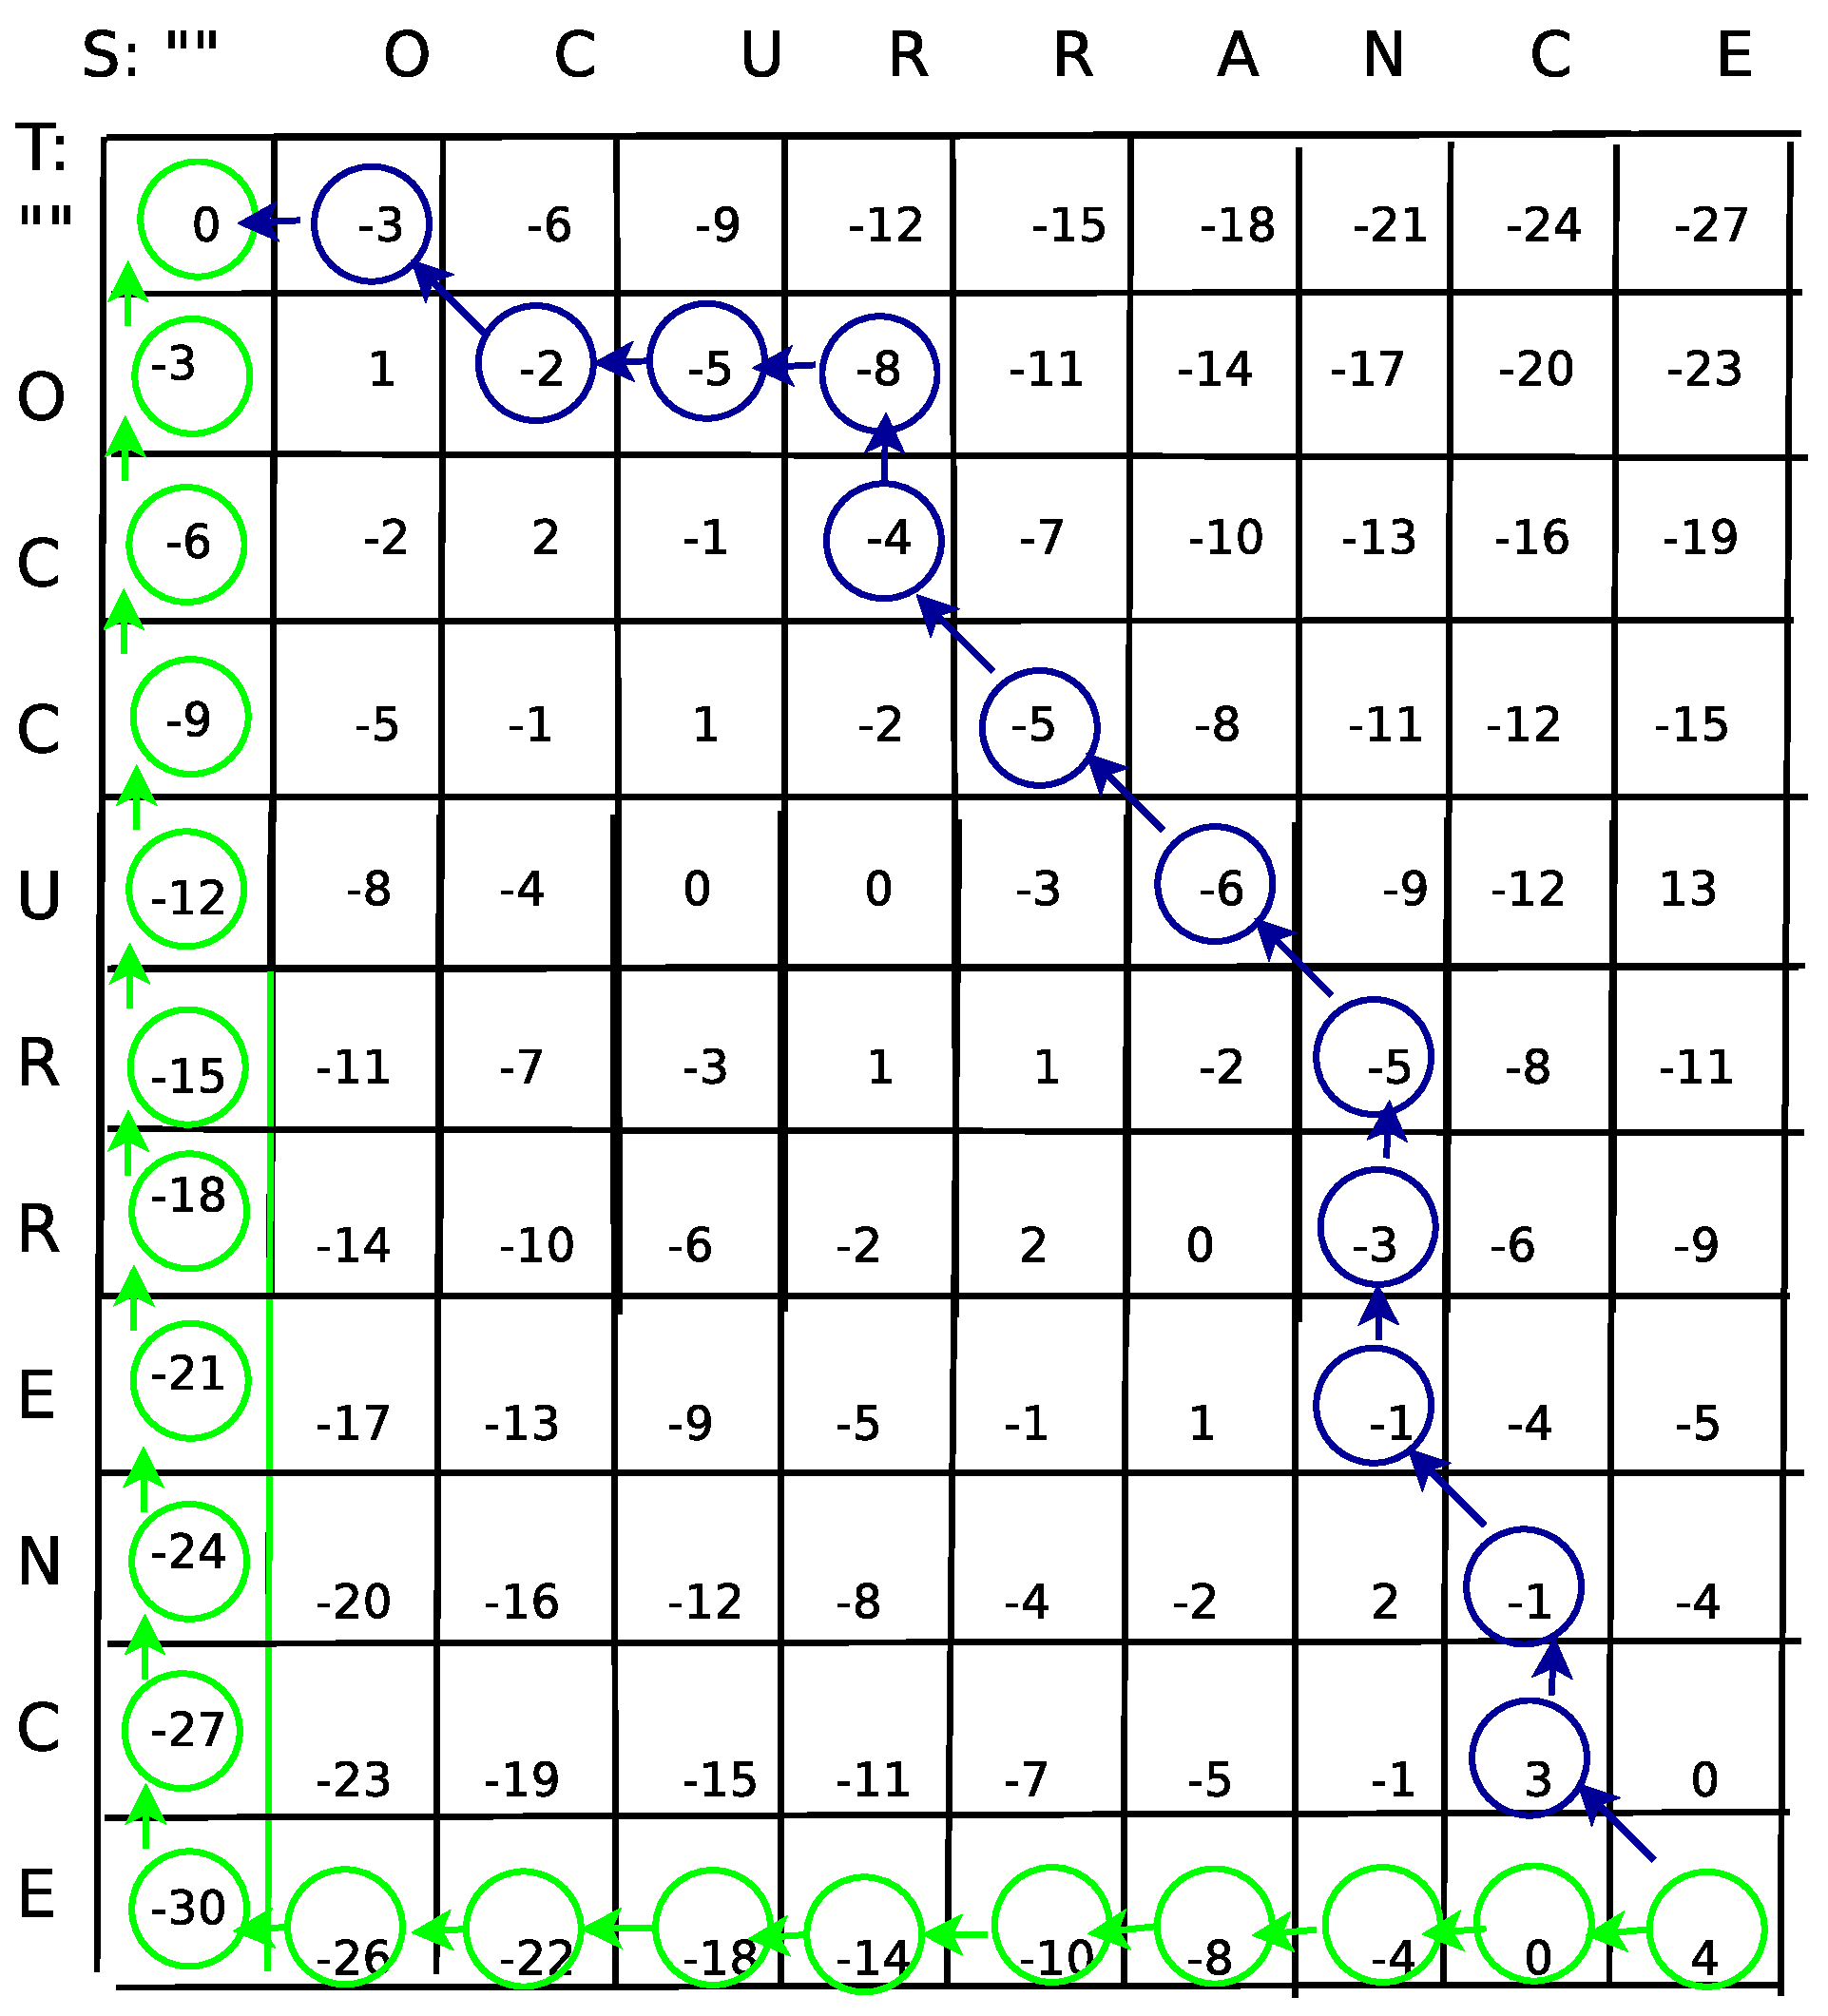
\includegraphics[width=2.in]{L6-occurence-alignments.eps}
%  \end{figure}
%  
%  \begin{tiny}
%  \begin{table}
%  \begin{tabular}{ll||ll}
%    \textcolor{green}{Alignment 1:}  &  \texttt{S'= ----------OCURRANCE }  & \textcolor{blue}{Alignment 2:}  &  \texttt{S'=OCUR-RAN---C-E } \\ 
%		    &	\texttt{T'=  OCCURRENCE--------- }  &   &\texttt{T'=-O---CCURRENCE } \\
%  \end{tabular} 
%  \end{table}
%  \end{tiny}  
%  Note: there are a total of ${m+n \choose m}$ possible alignments.
%}

\frame{
	\begin{block}{}
	Question: how to find the alignment with the highest score? 
	\end{block}
}

\frame{
\frametitle{Find the optimal alignment via \textcolor{red}{backtracking } }
%  \begin{figure}
%  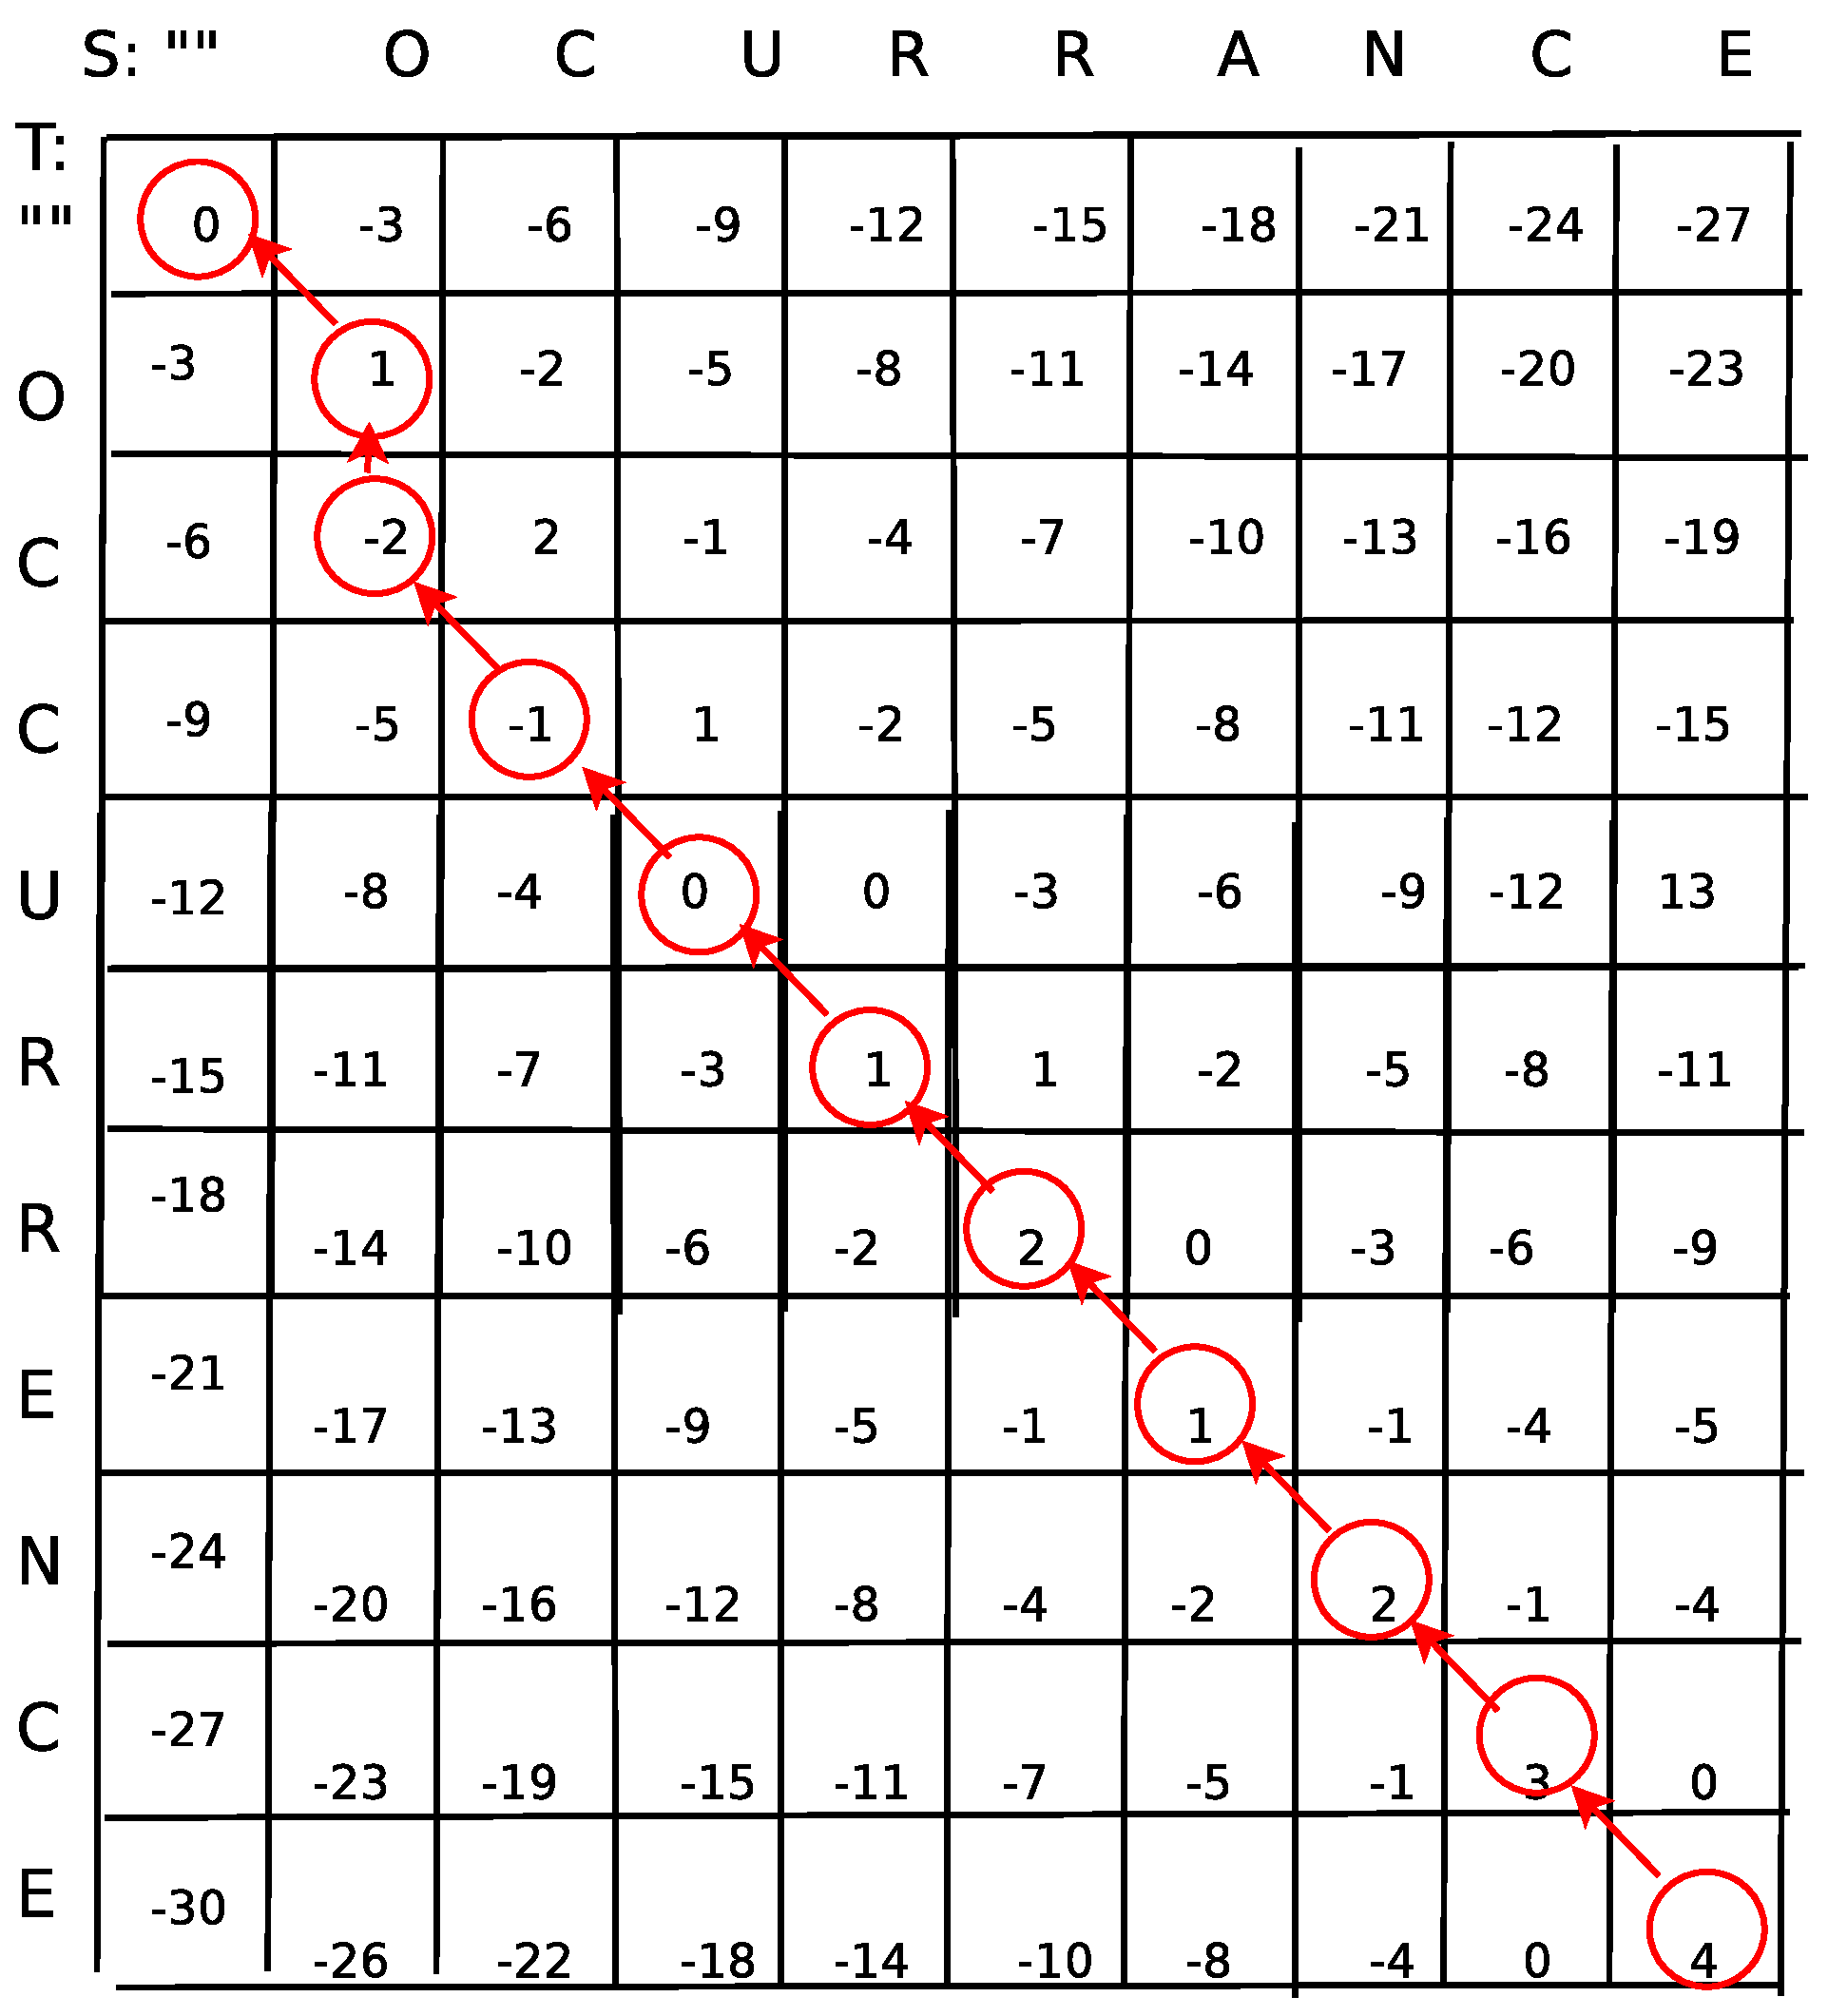
\includegraphics[width=2.1in]{L6-occurence-backtrack.eps}
%  \end{figure}
  
\begin{figure}
    
\begin{tikzpicture}[scale=0.78, auto,swap]
  
  	\def\d{0.7};
	
	%draw index 
 \def\dy{1};
 \def\dx{0};

    \foreach \i/\num/\name in {0/S:\ /, 1/''/s1,2/O/s2,3/C/s3,4/U/s4,5/R/,6/R/,7/A/,8/N/,9/C/,10/E/}{
           \node[blue,thick] (\name) at (\i*\d+\d/2 + \dx*\d - \d, \d/2 + \dy * \d) {\tt \num};
    }

 \def\dy{0};
 \def\dx{0};
    \foreach \i/\num/\name in {1/T:''/s1,2/O/s2,3/C/s3,4/C/s4, 5/U/,6/R/,7/R/,8/E/,9/N/,10/C/,11/E/}{
         \node[blue,thick] (\name) at ( -1*\d+\d/2  - 0.3,  0.0 - \i*\d + \d/2 - \dy * \d + \d){\tt  \num};
    }

    
%score	
 \def\dy{0};
 \def\dx{0};
    \foreach \i/\num/\name in {0/0/C,1/-3/S1,2/-6/S2,3/-9/,4/-12/,5/-15/,6/-18/,7/-21/,8/-24/,9/-27/}{
             \draw[  thick ] (\i*\d + \dx*\d,  0+ \dy*\d) rectangle (\i*\d+\d + \dx*\d, \d + \dy*\d);
         \node (\name) at (\i*\d+\d/2 + \dx*\d, \d/2 + \dy*\d) {\tiny $\num$};
    }
               \draw[red,ultra thick] (C) circle[radius=\d/2];

 \def\dy{-1};
 \def\dx{0};
    \foreach \i/\num/\name in {0/-3/,1/1/C,2/-2/,3/-5/LU,4/-8/U,5/-11/,6/-14/,7/-17/,8/-20/,9/-23/}{
             \draw[  thick ] (\i*\d + \dx*\d,  0+ \dy*\d) rectangle (\i*\d+\d + \dx*\d, \d + \dy*\d);
         \node (\name) at (\i*\d+\d/2 + \dx*\d, \d/2 + \dy*\d) {\tiny $\num$};
    }
                   \draw[red,ultra thick] (C) circle[radius=\d/2];

    
        
 \def\dy{-2};
 \def\dx{0};
    \foreach \i/\num/\name in {0/-6/,1/-2/C,2/2/,3/-1/L,4/-4/,5/-7/,6/-10/,7/-13/,8/-16/,9/-19/}{
             \draw[  thick ] (\i*\d + \dx*\d,  0+ \dy*\d) rectangle (\i*\d+\d + \dx*\d, \d + \dy*\d);
         \node (\name) at (\i*\d+\d/2 + \dx*\d, \d/2 + \dy*\d) {\tiny $\num$};
    }
                   \draw[red,ultra thick] (C) circle[radius=\d/2];



    
 \def\dy{-3};
 \def\dx{0};
    \foreach \i/\num/\name in {0/-9/,1/-5/,2/-1/C,3/1/S3,4/-2/,5/-5/,6/-8/,7/-11/,8/-12/,9/-15/}{
             \draw[  thick ] (\i*\d + \dx*\d,  0+ \dy*\d) rectangle (\i*\d+\d + \dx*\d, \d + \dy*\d);
         \node (\name) at (\i*\d+\d/2 + \dx*\d, \d/2 + \dy*\d) {\tiny $\num$};
    }
                   \draw[red,ultra thick] (C) circle[radius=\d/2];
                   
  \def\dy{-4};
 \def\dx{0};
    \foreach \i/\num/\name in {0/-12/,1/-8/,2/-4/,3/0/C,4/0/,5/-3/,6/-6/,7/-9/,8/-12/,9/-13/}{
             \draw[  thick ] (\i*\d + \dx*\d,  0+ \dy*\d) rectangle (\i*\d+\d + \dx*\d, \d + \dy*\d);
         \node (\name) at (\i*\d+\d/2 + \dx*\d, \d/2 + \dy*\d) {\tiny $\num$};
    }
                   \draw[red,ultra thick] (C) circle[radius=\d/2];
                   
  \def\dy{-5};
 \def\dx{0};
    \foreach \i/\num/\name in {0/-15/,1/-11/,2/-7/,3/-3/S3,4/1/C,5/1/,6/-2/,7/-5/,8/-8/,9/-11/}{
             \draw[  thick ] (\i*\d + \dx*\d,  0+ \dy*\d) rectangle (\i*\d+\d + \dx*\d, \d + \dy*\d);
         \node (\name) at (\i*\d+\d/2 + \dx*\d, \d/2 + \dy*\d) {\tiny $\num$};
    }
                   \draw[red,ultra thick] (C) circle[radius=\d/2];
                   
  \def\dy{-6};
 \def\dx{0};
    \foreach \i/\num/\name in {0/-18/,1/-14/,2/-10/,3/-6/S3,4/-2/,5/2/C,6/0/,7/-3/,8/-6/,9/-9/}{
             \draw[  thick ] (\i*\d + \dx*\d,  0+ \dy*\d) rectangle (\i*\d+\d + \dx*\d, \d + \dy*\d);
         \node (\name) at (\i*\d+\d/2 + \dx*\d, \d/2 + \dy*\d) {\tiny $\num$};
    }
               \draw[red,ultra thick] (C) circle[radius=\d/2];

    
  \def\dy{-7};
 \def\dx{0};
    \foreach \i/\num/\name in {0/-21/,1/-17/,2/-13/,3/-9/S3,4/-5/,5/-1/,6/1/C,7/-1/,8/-4/,9/-5/}{
             \draw[  thick ] (\i*\d + \dx*\d,  0+ \dy*\d) rectangle (\i*\d+\d + \dx*\d, \d + \dy*\d);
         \node (\name) at (\i*\d+\d/2 + \dx*\d, \d/2 + \dy*\d) {\tiny $\num$};
    }
               \draw[red,ultra thick] (C) circle[radius=\d/2];

    
  \def\dy{-8};
 \def\dx{0};
    \foreach \i/\num/\name in {0/-24/,1/-20/,2/-16/,3/-12/S3,4/-8/,5/-4/,6/-2/,7/2/C,8/-1/,9/-4/}{
             \draw[  thick ] (\i*\d + \dx*\d,  0+ \dy*\d) rectangle (\i*\d+\d + \dx*\d, \d + \dy*\d);
         \node (\name) at (\i*\d+\d/2 + \dx*\d, \d/2 + \dy*\d) {\tiny $\num$};
    }
               \draw[red,ultra thick] (C) circle[radius=\d/2];

  \def\dy{-9};
 \def\dx{0};
    \foreach \i/\num/\name in {0/-27/,1/-23/,2/-19/,3/-15/S3,4/-11/,5/-7/,6/-5/,7/-1/,8/3/C,9/0/U}{
             \draw[  thick ] (\i*\d + \dx*\d,  0+ \dy*\d) rectangle (\i*\d+\d + \dx*\d, \d + \dy*\d);
         \node (\name) at (\i*\d+\d/2 + \dx*\d, \d/2 + \dy*\d) {\tiny $\num$};
    }
               \draw[red,ultra thick] (C) circle[radius=\d/2];

  \def\dy{-10};
 \def\dx{0};
    \foreach \i/\num/\name in {0/-30/,1/-26/,2/-22/,3/-18/S3,4/-14/,5/-10/,6/-8/,7/-4/,8/0/L,9/4/C}{
             \draw[  thick ] (\i*\d + \dx*\d,  0+ \dy*\d) rectangle (\i*\d+\d + \dx*\d, \d + \dy*\d);
         \node (\name) at (\i*\d+\d/2 + \dx*\d, \d/2 + \dy*\d) {\tiny $\num$};
    }
           \draw[red,ultra thick] (C) circle[radius=\d/2];
                         


\end{tikzpicture} 
\end{figure}     


  
  \begin{tiny}
 
  \begin{table}
  \begin{tabular}{ll}
    Optimal Alignment:  &  \texttt{S'=  O-CURRANCE } \\ 
   		     &	\texttt{T'=  OCCURRENCE } \\
  \end{tabular} 
  \end{table}
  \end{tiny}  
}

\frame{
	\frametitle{Optimal alignment versus sub-optimal alignments }

\begin{itemize}
	\item  In practice, there are always multiple alignments with nearly the same score as the optimal alignment. Such alignments are called \textcolor{red}{\bf sub-optimal alignments} and can be divided into the following two categories. 
	\begin{itemize}
		\item Similar sub-optimal alignments: Some sub-optimal alignments differ from the optimal alignment in a few positions. Because variations might occur independently at different positions, the number of sub-optimal alignments grow exponentially with the difference to the optimal alignment. The typical sub-optimal alignments can be obtained through \textcolor{red}{\bf sampling} over the dynamic programming matrix. 
		\item Distinct sub-optimal alignments: The other sub-optimal alignments differ completely from the optimal alignment. These sub-optimal alignments frequently appear when one or both sequences have repeats. 
	\end{itemize}
\end{itemize} 
	Please refer to Biological Sequence Analysis: Probabilistic Models of Proteins and Nucleic Acids  for details. 

}

\frame{
	\frametitle{Finding  sub-optimal alignments}
	\begin{itemize}
		\item To find similar sub-optimal alignments, we trace back through the dynamic programming matrix using sampling technique, i.e., instead of taking the highest scoring option at each step, we make probabilistic choices bases on the value of the three options. 
		
		\item To find the next best alignment sharing no aligned residue pairs with the optimal alignment, we can re-calculate the dynamic programming matrix with cells corresponding to the pairs in the optimal alignment set to zero. The resulting matrix can be used to find the second best alignment. Another approach is extending cells of $OPT$ table to store top alignments. 

%		\item Take the example as shown above. We sample out the following alignments: 
%		
%		
%	We can see that alternatives occur  more likely at the beginning while pairings are more stable at the end of the sequences. By averaging over the sample, property of particular interest can be estimated. 
	\end{itemize}
}

%\frame{
%	\frametitle{Finding distinct sub-optimal alignments} 
%	
%	\begin{itemize}
%		\item To find the next best alignment sharing no aligned residue pairs with the optimal alignment, we can re-calculate the dynamic programming matrix with cells corresponding to the pairs in the optimal alignment set to zero. The resulting matrix can be used to find the second best alignment. 
%		
%	\end{itemize}
%}

\frame{
	\frametitle{Advanced DP} 
	
	\begin{itemize}
		\item Once have a basic DP algorithm, it is usually possible to make further improvement by saving running time and space requirement. 
		\item Saving space requirement: 
			\begin{itemize}
				\item In 1975, D. S. Hirschberg proposed to apply {\sc Divide-and-Conquer} technique to calculate optimal sequence alignment using only $O(m+n)$ space. J. Ian Munro improved this algorithm in 1982. 
				\item In 2018, F. Yang et al. proposed to use neural network to reduce the space requirement of {\sc Held-Karp} algorithm
			\end{itemize}

		\item Saving running time: 
			\begin{itemize}
				\item Exploring the \textcolor{red}{\bf location of optimal solution}: banded DP 
				\item Exploring the \textcolor{red}{\bf sparsity of memoization table}: sparse DP 
				\item Exploring the \textcolor{red}{\bf monotonicity of backtracking table} 
			\end{itemize}
	
	\end{itemize}

}

\frame{
\begin{block}{}
Space efficient algorithm: reducing the space requirement from $O(mn)$ to $O(m+n)$ using {\sc Divide-and-Conquer} (D. S. Hirschberg, 1975)
\end{block} 
} 

\frame{
\frametitle{Technique 1: two arrays are enough if only score is needed}
\begin{itemize}
\item Key observation 1: it is easy to calculate \textcolor{blue}{\bf the final score $OPT(T, S)$ only}, i.e. \textcolor{blue}{\bf the alignment information are not recorded.}
\end{itemize}

%  \begin{figure}
%  \includegraphics[width=2.2in]{L6-occurencestep2.eps}
%  \end{figure}
 	\begin{figure}
    
\begin{tikzpicture}[scale=0.78, auto,swap]
  
  	\def\d{0.7};
	
	%draw index 
 \def\dy{1};
 \def\dx{0};

    \foreach \i/\num/\name in {0/S:\ /, 1/''/s1,2/O/s2,3/C/s3,4/U/s4,5/R/,6/R/,7/A/,8/N/,9/C/,10/E/}{
           \node[blue,thick] (\name) at (\i*\d+\d/2 + \dx*\d - \d, \d/2 + \dy * \d) {\tt \num};
    }

 \def\dy{0};
 \def\dx{0};
    \foreach \i/\num/\name in {1/T:''/s1,2/O/s2,3/C/s3,4/C/s4, 5/U/,6/R/,7/R/,8/E/,9/N/,10/C/,11/E/}{
         \node[blue,thick] (\name) at ( -1*\d+\d/2 - 0.3,  0.0 - \i*\d + \d/2 - \dy * \d + \d){\tt  \num};
    }

    
%score	
 \def\dy{0};
 \def\dx{0};
    \foreach \i/\num/\name in {0/0/,1/-3/S1,2/-6/S2,3/-9/,4/-12/,5/-15/,6/-18/,7/-21/,8/-24/,9/-27/}{
             \draw[  thick ] (\i*\d + \dx*\d,  0+ \dy*\d) rectangle (\i*\d+\d + \dx*\d, \d + \dy*\d);
         \node (\name) at (\i*\d+\d/2 + \dx*\d, \d/2 + \dy*\d) {\tiny $\num$};
    }


 \def\dy{-1};
 \def\dx{0};
    \foreach \i/\num/\name in {0/-3/,1/1/,2/-2/C,3/-5/LU,4/-8/U,5/-11/,6/-14/,7/-17/,8/-20/,9/-23/}{
             \draw[  thick ] (\i*\d + \dx*\d,  0+ \dy*\d) rectangle (\i*\d+\d + \dx*\d, \d + \dy*\d);
         \node (\name) at (\i*\d+\d/2 + \dx*\d, \d/2 + \dy*\d) {\tiny $\num$};
    }
    

    
        
 \def\dy{-2};
 \def\dx{0};
    \foreach \i/\num/\name in {0/-6/,1/-2/,2/2/,3/-1/L,4/-4/C,5/-7/,6/-10/,7/-13/,8/-16/,9/-19/}{
             \draw[  thick ] (\i*\d + \dx*\d,  0+ \dy*\d) rectangle (\i*\d+\d + \dx*\d, \d + \dy*\d);
         \node (\name) at (\i*\d+\d/2 + \dx*\d, \d/2 + \dy*\d) {\tiny $\num$};
    }
    



    
 \def\dy{-3};
 \def\dx{0};
    \foreach \i/\num/\name in {0/-9/,1/-5/,2/-1/,3/1/S3,4/-2/,5/-5/,6/-8/,7/-11/,8/-12/,9/-15/}{
             \draw[  thick ] (\i*\d + \dx*\d,  0+ \dy*\d) rectangle (\i*\d+\d + \dx*\d, \d + \dy*\d);
         \node (\name) at (\i*\d+\d/2 + \dx*\d, \d/2 + \dy*\d) {\tiny $\num$};
    }
    
  \def\dy{-4};
 \def\dx{0};
    \foreach \i/\num/\name in {0/-12/,1/-8/,2/-4/,3/0/S3,4/0/,5/-3/,6/-6/,7/-9/,8/-12/,9/-13/}{
             \draw[  thick ] (\i*\d + \dx*\d,  0+ \dy*\d) rectangle (\i*\d+\d + \dx*\d, \d + \dy*\d);
         \node (\name) at (\i*\d+\d/2 + \dx*\d, \d/2 + \dy*\d) {\tiny $\num$};
    }
    
  \def\dy{-5};
 \def\dx{0};
    \foreach \i/\num/\name in {0/-15/,1/-11/,2/-7/,3/-3/S3,4/1/,5/1/,6/-2/,7/-5/,8/-8/,9/-11/}{
             \draw[  thick ] (\i*\d + \dx*\d,  0+ \dy*\d) rectangle (\i*\d+\d + \dx*\d, \d + \dy*\d);
         \node (\name) at (\i*\d+\d/2 + \dx*\d, \d/2 + \dy*\d) {\tiny $\num$};
    }
    
  \def\dy{-6};
 \def\dx{0};
    \foreach \i/\num/\name in {0/-18/,1/-14/,2/-10/,3/-6/S3,4/-2/,5/2/,6/0/,7/-3/,8/-6/,9/-9/}{
             \draw[  thick ] (\i*\d + \dx*\d,  0+ \dy*\d) rectangle (\i*\d+\d + \dx*\d, \d + \dy*\d);
         \node (\name) at (\i*\d+\d/2 + \dx*\d, \d/2 + \dy*\d) {\tiny $\num$};
    }
    
  \def\dy{-7};
 \def\dx{0};
    \foreach \i/\num/\name in {0/-21/,1/-17/,2/-13/,3/-9/S3,4/-5/,5/-1/,6/1/,7/-1/,8/-4/,9/-5/}{
             \draw[  thick ] (\i*\d + \dx*\d,  0+ \dy*\d) rectangle (\i*\d+\d + \dx*\d, \d + \dy*\d);
         \node (\name) at (\i*\d+\d/2 + \dx*\d, \d/2 + \dy*\d) {\tiny $\num$};
    }
    
  \def\dy{-8};
 \def\dx{0};
    \foreach \i/\num/\name in {0/-24/,1/-20/,2/-16/,3/-12/S3,4/-8/,5/-4/,6/-2/,7/2/,8/-1/,9/-4/}{
             \draw[  thick ] (\i*\d + \dx*\d,  0+ \dy*\d) rectangle (\i*\d+\d + \dx*\d, \d + \dy*\d);
         \node (\name) at (\i*\d+\d/2 + \dx*\d, \d/2 + \dy*\d) {\tiny $\num$};
    }
    
  \def\dy{-9};
 \def\dx{0};
    \foreach \i/\num/\name in {0/-27/,1/-23/,2/-19/,3/-15/S3,4/-11/,5/-7/,6/-5/,7/-1/,8/3/LU,9/0/U}{
             \draw[  thick ] (\i*\d + \dx*\d,  0+ \dy*\d) rectangle (\i*\d+\d + \dx*\d, \d + \dy*\d);
         \node (\name) at (\i*\d+\d/2 + \dx*\d, \d/2 + \dy*\d) {\tiny $\num$};
    }
    
  \def\dy{-10};
 \def\dx{0};
    \foreach \i/\num/\name in {0/-30/,1/-26/,2/-22/,3/-18/S3,4/-14/,5/-10/,6/-8/,7/-4/,8/0/L,9/4/C}{
             \draw[  thick ] (\i*\d + \dx*\d,  0+ \dy*\d) rectangle (\i*\d+\d + \dx*\d, \d + \dy*\d);
         \node (\name) at (\i*\d+\d/2 + \dx*\d, \d/2 + \dy*\d) {\tiny $\num$};
    }
    
    
           \draw[red,ultra thick] (C) circle[radius=\d/2];
%   \draw[blue,ultra thick] (U) circle[radius=\d/2];
%   \draw[blue,ultra thick] (LU) circle[radius=\d/2];
%   \draw[blue,ultra thick] (L) circle[radius=\d/2];                                


\end{tikzpicture} 
\end{figure}     


} 

\frame{
\frametitle{Technique 1: two arrays are enough if only score is needed}
\begin{itemize}
\item \begin{small}  Why? Only column $j-1$ is needed to calculate column $j$. Thus, we use two arrays $score[1..m]$ and $newscore[1..m]$ instead of the matrix $OPT[1..m,1..n]$. \end{small} 
\end{itemize}

%  \begin{figure}
%  \includegraphics[width=2.2in]{L6-occurencespaceefficientstep0.eps}
%  \end{figure}

 \begin{figure}
 \begin{tikzpicture}[scale=0.78, auto,swap]
  
  	\def\d{0.7};
	
	%draw index 
 \def\dy{1};
 \def\dx{0};

    \foreach \i/\num/\name in {-0.5/\ S:\ /, 1/''/s1,2/O/s2,3/C/s3,4/U/s4,5/R/,6/R/,7/A/,8/N/,9/C/,10/E/}{
           \node[blue,thick] (\name) at (\i*\d+\d/2 + \dx*\d - \d, \d/2 + \dy * \d) {\tt \num};
    }

 \def\dy{0};
 \def\dx{0};
    \foreach \i/\num/\name in {1/T:\ ''/s1,2/O/s2,3/C/s3,4/C/s4, 5/U/,6/R/,7/R/,8/E/,9/N/,10/C/,11/E/}{
         \node[blue,thick] (\name) at ( -1*\d+\d/2-0.3,  0.0 - \i*\d + \d/2 - \dy * \d + \d){\tt  \num};
    }

    
%score	
 \def\dy{0};
 \def\dx{0};
    \foreach \i/\num/\name/\color in {0/0/S00/green,1/-3/S01/blue!20,2/-6/S2/white,3/-9//white,4/-12//white,5/-15//white,6/-18//white,7/-21//white,8/-24//white,9/-27//white}{
             \draw[  thick, fill=\color ] (\i*\d + \dx*\d,  0+ \dy*\d) rectangle (\i*\d+\d + \dx*\d, \d + \dy*\d);
         \node (\name) at (\i*\d+\d/2 + \dx*\d, \d/2 + \dy*\d) {\tiny $\num$};
    }


 \def\dy{-1};
 \def\dx{0};
    \foreach \i/\num/\name/\color in {0/-3//green,1/1//blue!20,2/-2/C/white,3/-5/LU/white,4/-8/U/white,5/-11//white,6/-14//white,7/-17//white,8/-20//white,9/-23//white}{
             \draw[  thick, fill=\color ] (\i*\d + \dx*\d,  0+ \dy*\d) rectangle (\i*\d+\d + \dx*\d, \d + \dy*\d);
         \node (\name) at (\i*\d+\d/2 + \dx*\d, \d/2 + \dy*\d) {\tiny $\num$};
    }
    

    
        
 \def\dy{-2};
 \def\dx{0};
    \foreach \i/\num/\name/\color in {0/-6//green,1/-2//blue!20,2/2//white,3/-1/L/white,4/-4/C/white,5/-7//white,6/-10//white,7/-13//white,8/-16//white,9/-19//white}{
             \draw[  thick, fill=\color ] (\i*\d + \dx*\d,  0+ \dy*\d) rectangle (\i*\d+\d + \dx*\d, \d + \dy*\d);
         \node (\name) at (\i*\d+\d/2 + \dx*\d, \d/2 + \dy*\d) {\tiny $\num$};
    }
    



    
 \def\dy{-3};
 \def\dx{0};
    \foreach \i/\num/\name/\color in {0/-9//green,1/-5//blue!20,2/-1//white,3/1/S3/white,4/-2/white,5/-5//white,6/-8//white,7/-11//white,8/-12//white,9/-15//white}{
             \draw[  thick, fill=\color ] (\i*\d + \dx*\d,  0+ \dy*\d) rectangle (\i*\d+\d + \dx*\d, \d + \dy*\d);
         \node (\name) at (\i*\d+\d/2 + \dx*\d, \d/2 + \dy*\d) {\tiny $\num$};
    }
    
  \def\dy{-4};
 \def\dx{0};
    \foreach \i/\num/\name/\color in {0/-12//green,1/-8//blue!20,2/-4//white,3/0/S3/white,4/0//white,5/-3//white,6/-6//white,7/-9//white,8/-12//white,9/-13//white}{
             \draw[  thick, fill=\color ] (\i*\d + \dx*\d,  0+ \dy*\d) rectangle (\i*\d+\d + \dx*\d, \d + \dy*\d);
         \node (\name) at (\i*\d+\d/2 + \dx*\d, \d/2 + \dy*\d) {\tiny $\num$};
    }
    
  \def\dy{-5};
 \def\dx{0};
    \foreach \i/\num/\name/\color in {0/-15//green,1/-11//blue!20,2/-7//white,3/-3/S3/white,4/1//white,5/1//white,6/-2//white,7/-5//white,8/-8//white,9/-11//white}{
             \draw[  thick, fill=\color ] (\i*\d + \dx*\d,  0+ \dy*\d) rectangle (\i*\d+\d + \dx*\d, \d + \dy*\d);
         \node (\name) at (\i*\d+\d/2 + \dx*\d, \d/2 + \dy*\d) {\tiny $\num$};
    }
    
  \def\dy{-6};
 \def\dx{0};
    \foreach \i/\num/\name/\color in {0/-18//green,1/-14//blue!20,2/-10//white,3/-6/S3/white,4/-2//white,5/2//white,6/0//white,7/-3//white,8/-6//white,9/-9//white}{
             \draw[  thick, fill=\color ] (\i*\d + \dx*\d,  0+ \dy*\d) rectangle (\i*\d+\d + \dx*\d, \d + \dy*\d);
         \node (\name) at (\i*\d+\d/2 + \dx*\d, \d/2 + \dy*\d) {\tiny $\num$};
    }
    
  \def\dy{-7};
 \def\dx{0};
    \foreach \i/\num/\name/\color in {0/-21//green,1/-17//blue!20,2/-13//white,3/-9/S3/white,4/-5//white,5/-1//white,6/1//white,7/-1//white,8/-4//white,9/-5//white}{
             \draw[  thick, fill=\color ] (\i*\d + \dx*\d,  0+ \dy*\d) rectangle (\i*\d+\d + \dx*\d, \d + \dy*\d);
         \node (\name) at (\i*\d+\d/2 + \dx*\d, \d/2 + \dy*\d) {\tiny $\num$};
    }
    
  \def\dy{-8};
 \def\dx{0};
    \foreach \i/\num/\name/\color in {0/-24//green,1/-20//blue!20,2/-16//white,3/-12/S3/white,4/-8//white,5/-4//white,6/-2//white,7/2//white,8/-1//white,9/-4//white}{
             \draw[  thick, fill=\color ] (\i*\d + \dx*\d,  0+ \dy*\d) rectangle (\i*\d+\d + \dx*\d, \d + \dy*\d);
         \node (\name) at (\i*\d+\d/2 + \dx*\d, \d/2 + \dy*\d) {\tiny $\num$};
    }
    
  \def\dy{-9};
 \def\dx{0};
    \foreach \i/\num/\name/\color in {0/-27//green,1/-23//blue!20,2/-19//white,3/-15/S3/white,4/-11//white,5/-7//white,6/-5//white,7/-1//white,8/3/LU/white,9/0/U/white}{
             \draw[  thick, fill=\color ] (\i*\d + \dx*\d,  0+ \dy*\d) rectangle (\i*\d+\d + \dx*\d, \d + \dy*\d);
         \node (\name) at (\i*\d+\d/2 + \dx*\d, \d/2 + \dy*\d) {\tiny $\num$};
    }
    
  \def\dy{-10};
 \def\dx{0};
    \foreach \i/\num/\name/\color in {0/-30/Sn0/green,1/-26/Sn1/blue!20,2/-22//white,3/-18/S3/white,4/-14//white,5/-10//white,6/-8//white,7/-4//white,8/0/L/white,9/4/C/white}{
             \draw[  thick, fill=\color ] (\i*\d + \dx*\d,  0+ \dy*\d) rectangle (\i*\d+\d + \dx*\d, \d + \dy*\d);
         \node (\name) at (\i*\d+\d/2 + \dx*\d, \d/2 + \dy*\d) {\tiny $\num$};
    }
    

%    \draw[green, thick] (S00.north west) rectangle (Sn0.south east);
%     \draw[blue, thick] (S01.north west) rectangle (Sn1.south east);
     
     
\end{tikzpicture} 
\end{figure}     


} 

\frame{
\frametitle{Technique 1: two arrays are enough if only score is needed}
\begin{itemize}
\item \begin{small}  Why? Only column $j-1$ is needed to calculate column $i$. Thus, we use two arrays $score[1..n]$ and $newscore[1..n]$ instead of the matrix $OPT[1..n,1..m]$. \end{small} 
\end{itemize}

%  \begin{figure}
%  \includegraphics[width=2.2in]{L6-occurencespaceefficientstep1.eps}
%  \end{figure}




 \begin{figure}
 \begin{tikzpicture}[scale=0.78, auto,swap]
  
  	\def\d{0.7};
	
	%draw index 
 \def\dy{1};
 \def\dx{0};

    \foreach \i/\num/\name in {-0.5/\ S:\ /, 1/''/s1,2/O/s2,3/C/s3,4/U/s4,5/R/,6/R/,7/A/,8/N/,9/C/,10/E/}{
           \node[blue,thick] (\name) at (\i*\d+\d/2 + \dx*\d - \d, \d/2 + \dy * \d) {\tt \num};
    }

 \def\dy{0};
 \def\dx{0};
    \foreach \i/\num/\name in {1/T:\ ''/s1,2/O/s2,3/C/s3,4/C/s4, 5/U/,6/R/,7/R/,8/E/,9/N/,10/C/,11/E/}{
         \node[blue,thick] (\name) at ( -1*\d+\d/2-0.3,  0.0 - \i*\d + \d/2 - \dy * \d + \d){\tt  \num};
    }

    
%score	
 \def\dy{0};
 \def\dx{0};
    \foreach \i/\num/\name/\color in {0/0/S00/white,1/-3/S01/green,2/-6/S2/blue!20,3/-9//white,4/-12//white,5/-15//white,6/-18//white,7/-21//white,8/-24//white,9/-27//white}{
             \draw[  thick, fill=\color ] (\i*\d + \dx*\d,  0+ \dy*\d) rectangle (\i*\d+\d + \dx*\d, \d + \dy*\d);
         \node (\name) at (\i*\d+\d/2 + \dx*\d, \d/2 + \dy*\d) {\tiny $\num$};
    }


 \def\dy{-1};
 \def\dx{0};
    \foreach \i/\num/\name/\color in {0/-3//white,1/1//green,2/-2/C/blue!20,3/-5/LU/white,4/-8/U/white,5/-11//white,6/-14//white,7/-17//white,8/-20//white,9/-23//white}{
             \draw[  thick, fill=\color ] (\i*\d + \dx*\d,  0+ \dy*\d) rectangle (\i*\d+\d + \dx*\d, \d + \dy*\d);
         \node (\name) at (\i*\d+\d/2 + \dx*\d, \d/2 + \dy*\d) {\tiny $\num$};
    }
    

    
        
 \def\dy{-2};
 \def\dx{0};
    \foreach \i/\num/\name/\color in {0/-6//white,1/-2//green,2/2//blue!20,3/-1/L/white,4/-4/C/white,5/-7//white,6/-10//white,7/-13//white,8/-16//white,9/-19//white}{
             \draw[  thick, fill=\color ] (\i*\d + \dx*\d,  0+ \dy*\d) rectangle (\i*\d+\d + \dx*\d, \d + \dy*\d);
         \node (\name) at (\i*\d+\d/2 + \dx*\d, \d/2 + \dy*\d) {\tiny $\num$};
    }
    



    
 \def\dy{-3};
 \def\dx{0};
    \foreach \i/\num/\name/\color in {0/-9//white,1/-5//green,2/-1//blue!20,3/1/S3/white,4/-2/white,5/-5//white,6/-8//white,7/-11//white,8/-12//white,9/-15//white}{
             \draw[  thick, fill=\color ] (\i*\d + \dx*\d,  0+ \dy*\d) rectangle (\i*\d+\d + \dx*\d, \d + \dy*\d);
         \node (\name) at (\i*\d+\d/2 + \dx*\d, \d/2 + \dy*\d) {\tiny $\num$};
    }
    
  \def\dy{-4};
 \def\dx{0};
    \foreach \i/\num/\name/\color in {0/-12//white,1/-8//green,2/-4//blue!20,3/0/S3/white,4/0//white,5/-3//white,6/-6//white,7/-9//white,8/-12//white,9/-13//white}{
             \draw[  thick, fill=\color ] (\i*\d + \dx*\d,  0+ \dy*\d) rectangle (\i*\d+\d + \dx*\d, \d + \dy*\d);
         \node (\name) at (\i*\d+\d/2 + \dx*\d, \d/2 + \dy*\d) {\tiny $\num$};
    }
    
  \def\dy{-5};
 \def\dx{0};
    \foreach \i/\num/\name/\color in {0/-15//white,1/-11//green,2/-7//blue!20,3/-3/S3/white,4/1//white,5/1//white,6/-2//white,7/-5//white,8/-8//white,9/-11//white}{
             \draw[  thick, fill=\color ] (\i*\d + \dx*\d,  0+ \dy*\d) rectangle (\i*\d+\d + \dx*\d, \d + \dy*\d);
         \node (\name) at (\i*\d+\d/2 + \dx*\d, \d/2 + \dy*\d) {\tiny $\num$};
    }
    
  \def\dy{-6};
 \def\dx{0};
    \foreach \i/\num/\name/\color in {0/-18//white,1/-14//green,2/-10//blue!20,3/-6/S3/white,4/-2//white,5/2//white,6/0//white,7/-3//white,8/-6//white,9/-9//white}{
             \draw[  thick, fill=\color ] (\i*\d + \dx*\d,  0+ \dy*\d) rectangle (\i*\d+\d + \dx*\d, \d + \dy*\d);
         \node (\name) at (\i*\d+\d/2 + \dx*\d, \d/2 + \dy*\d) {\tiny $\num$};
    }
    
  \def\dy{-7};
 \def\dx{0};
    \foreach \i/\num/\name/\color in {0/-21//white,1/-17//green,2/-13//blue!20,3/-9/S3/white,4/-5//white,5/-1//white,6/1//white,7/-1//white,8/-4//white,9/-5//white}{
             \draw[  thick, fill=\color ] (\i*\d + \dx*\d,  0+ \dy*\d) rectangle (\i*\d+\d + \dx*\d, \d + \dy*\d);
         \node (\name) at (\i*\d+\d/2 + \dx*\d, \d/2 + \dy*\d) {\tiny $\num$};
    }
    
  \def\dy{-8};
 \def\dx{0};
    \foreach \i/\num/\name/\color in {0/-24//white,1/-20//green,2/-16//blue!20,3/-12/S3/white,4/-8//white,5/-4//white,6/-2//white,7/2//white,8/-1//white,9/-4//white}{
             \draw[  thick, fill=\color ] (\i*\d + \dx*\d,  0+ \dy*\d) rectangle (\i*\d+\d + \dx*\d, \d + \dy*\d);
         \node (\name) at (\i*\d+\d/2 + \dx*\d, \d/2 + \dy*\d) {\tiny $\num$};
    }
    
  \def\dy{-9};
 \def\dx{0};
    \foreach \i/\num/\name/\color in {0/-27//white,1/-23//green,2/-19//blue!20,3/-15/S3/white,4/-11//white,5/-7//white,6/-5//white,7/-1//white,8/3/LU/white,9/0/U/white}{
             \draw[  thick, fill=\color ] (\i*\d + \dx*\d,  0+ \dy*\d) rectangle (\i*\d+\d + \dx*\d, \d + \dy*\d);
         \node (\name) at (\i*\d+\d/2 + \dx*\d, \d/2 + \dy*\d) {\tiny $\num$};
    }
    
  \def\dy{-10};
 \def\dx{0};
    \foreach \i/\num/\name/\color in {0/-30/Sn0/white,1/-26/Sn1/green,2/-22//blue!20,3/-18/S3/white,4/-14//white,5/-10//white,6/-8//white,7/-4//white,8/0/L/white,9/4/C/white}{
             \draw[  thick, fill=\color ] (\i*\d + \dx*\d,  0+ \dy*\d) rectangle (\i*\d+\d + \dx*\d, \d + \dy*\d);
         \node (\name) at (\i*\d+\d/2 + \dx*\d, \d/2 + \dy*\d) {\tiny $\num$};
    }
    

%    \draw[green, thick] (S00.north west) rectangle (Sn0.south east);
%     \draw[blue, thick] (S01.north west) rectangle (Sn1.south east);
     
     
\end{tikzpicture} 
\end{figure}     


} 

\frame{
\frametitle{Technique 1: two arrays are enough if only score is needed}
\begin{itemize}
\item \begin{small}  Why? Only column $j-1$ is needed to calculate column $i$. Thus, we use two arrays $score[0..m]$ and $newscore[0..m]$ instead of the matrix $OPT[0..m,0..n]$. \end{small} 
\end{itemize}

%  \begin{figure}
%  \includegraphics[width=2.2in]{L6-occurencespaceefficientstep2.eps}
%  \end{figure}



 \begin{figure}
 \begin{tikzpicture}[scale=0.78, auto,swap]
  
  	\def\d{0.7};
	
	%draw index 
 \def\dy{1};
 \def\dx{0};

    \foreach \i/\num/\name in {-0.5/\ S:\ /, 1/''/s1,2/O/s2,3/C/s3,4/U/s4,5/R/,6/R/,7/A/,8/N/,9/C/,10/E/}{
           \node[blue,thick] (\name) at (\i*\d+\d/2 + \dx*\d - \d, \d/2 + \dy * \d) {\tt \num};
    }

 \def\dy{0};
 \def\dx{0};
    \foreach \i/\num/\name in {1/T:\ ''/s1,2/O/s2,3/C/s3,4/C/s4, 5/U/,6/R/,7/R/,8/E/,9/N/,10/C/,11/E/}{
         \node[blue,thick] (\name) at ( -1*\d+\d/2-0.3,  0.0 - \i*\d + \d/2 - \dy * \d + \d){\tt  \num};
    }

    
%score
 \def\dy{0};
 \def\dx{0};
    \foreach \i/\num/\name/\color in {0/0/S00/white,1/-3/S01/white,2/-6/S2/white,3/-9//white,4/-12//white,5/-15//white,6/-18//white,7/-21//white,8/-24//green,9/-27//blue!20}{
             \draw[  thick, fill=\color ] (\i*\d + \dx*\d,  0+ \dy*\d) rectangle (\i*\d+\d + \dx*\d, \d + \dy*\d);
         \node (\name) at (\i*\d+\d/2 + \dx*\d, \d/2 + \dy*\d) {\tiny $\num$};
    }


 \def\dy{-1};
 \def\dx{0};
    \foreach \i/\num/\name/\color in {0/-3//white,1/1//white,2/-2/C/white,3/-5/LU/white,4/-8/U/white,5/-11//white,6/-14//white,7/-17//white,8/-20//green,9/-23//blue!20}{
             \draw[  thick, fill=\color ] (\i*\d + \dx*\d,  0+ \dy*\d) rectangle (\i*\d+\d + \dx*\d, \d + \dy*\d);
         \node (\name) at (\i*\d+\d/2 + \dx*\d, \d/2 + \dy*\d) {\tiny $\num$};
    }
    

    
        
 \def\dy{-2};
 \def\dx{0};
    \foreach \i/\num/\name/\color in {0/-6//white,1/-2//white,2/2//white,3/-1/L/white,4/-4/C/white,5/-7//white,6/-10//white,7/-13//white,8/-16//green,9/-19//blue!20}{
             \draw[  thick, fill=\color ] (\i*\d + \dx*\d,  0+ \dy*\d) rectangle (\i*\d+\d + \dx*\d, \d + \dy*\d);
         \node (\name) at (\i*\d+\d/2 + \dx*\d, \d/2 + \dy*\d) {\tiny $\num$};
    }
    
    
 \def\dy{-3};
 \def\dx{0};
    \foreach \i/\num/\name/\color in {0/-9//white,1/-5//white,2/-1//white,3/1/S3/white,4/-2/white,5/-5//white,6/-8//white,7/-11//white,8/-12//green,9/-15//blue!20}{
             \draw[  thick, fill=\color ] (\i*\d + \dx*\d,  0+ \dy*\d) rectangle (\i*\d+\d + \dx*\d, \d + \dy*\d);
         \node (\name) at (\i*\d+\d/2 + \dx*\d, \d/2 + \dy*\d) {\tiny $\num$};
    }
    
  \def\dy{-4};
 \def\dx{0};
    \foreach \i/\num/\name/\color in {0/-12//white,1/-8//white,2/-4//white,3/0/S3/white,4/0//white,5/-3//white,6/-6//white,7/-9//white,8/-12//green,9/-13//blue!20}{
             \draw[  thick, fill=\color ] (\i*\d + \dx*\d,  0+ \dy*\d) rectangle (\i*\d+\d + \dx*\d, \d + \dy*\d);
         \node (\name) at (\i*\d+\d/2 + \dx*\d, \d/2 + \dy*\d) {\tiny $\num$};
    }
    
  \def\dy{-5};
 \def\dx{0};
    \foreach \i/\num/\name/\color in {0/-15//white,1/-11//white,2/-7//white,3/-3/S3/white,4/1//white,5/1//white,6/-2//white,7/-5//white,8/-8//green,9/-11//blue!20}{
             \draw[  thick, fill=\color ] (\i*\d + \dx*\d,  0+ \dy*\d) rectangle (\i*\d+\d + \dx*\d, \d + \dy*\d);
         \node (\name) at (\i*\d+\d/2 + \dx*\d, \d/2 + \dy*\d) {\tiny $\num$};
    }
    
  \def\dy{-6};
 \def\dx{0};
    \foreach \i/\num/\name/\color in {0/-18//white,1/-14//white,2/-10//white,3/-6/S3/white,4/-2//white,5/2//white,6/0//white,7/-3//white,8/-6//green,9/-9//blue!20}{
             \draw[  thick, fill=\color ] (\i*\d + \dx*\d,  0+ \dy*\d) rectangle (\i*\d+\d + \dx*\d, \d + \dy*\d);
         \node (\name) at (\i*\d+\d/2 + \dx*\d, \d/2 + \dy*\d) {\tiny $\num$};
    }
    
  \def\dy{-7};
 \def\dx{0};
    \foreach \i/\num/\name/\color in {0/-21//white,1/-17//white,2/-13//white,3/-9/S3/white,4/-5//white,5/-1//white,6/1//white,7/-1//white,8/-4//green,9/-5//blue!20}{
             \draw[  thick, fill=\color ] (\i*\d + \dx*\d,  0+ \dy*\d) rectangle (\i*\d+\d + \dx*\d, \d + \dy*\d);
         \node (\name) at (\i*\d+\d/2 + \dx*\d, \d/2 + \dy*\d) {\tiny $\num$};
    }
    
  \def\dy{-8};
 \def\dx{0};
    \foreach \i/\num/\name/\color in {0/-24//white,1/-20//white,2/-16//white,3/-12/S3/white,4/-8//white,5/-4//white,6/-2//white,7/2//white,8/-1//green,9/-4//blue!20}{
             \draw[  thick, fill=\color ] (\i*\d + \dx*\d,  0+ \dy*\d) rectangle (\i*\d+\d + \dx*\d, \d + \dy*\d);
         \node (\name) at (\i*\d+\d/2 + \dx*\d, \d/2 + \dy*\d) {\tiny $\num$};
    }
    
  \def\dy{-9};
 \def\dx{0};
    \foreach \i/\num/\name/\color in {0/-27//white,1/-23//white,2/-19//white,3/-15/S3/white,4/-11//white,5/-7//white,6/-5//white,7/-1//white,8/3/LU/green,9/0/U/blue!20}{
             \draw[  thick, fill=\color ] (\i*\d + \dx*\d,  0+ \dy*\d) rectangle (\i*\d+\d + \dx*\d, \d + \dy*\d);
         \node (\name) at (\i*\d+\d/2 + \dx*\d, \d/2 + \dy*\d) {\tiny $\num$};
    }
    
  \def\dy{-10};
 \def\dx{0};
    \foreach \i/\num/\name/\color in {0/-30/Sn0/white,1/-26/Sn1/white,2/-22//white,3/-18/S3/white,4/-14//white,5/-10//white,6/-8//white,7/-4//white,8/0/L/green,9/4/C/blue!20}{
             \draw[  thick, fill=\color ] (\i*\d + \dx*\d,  0+ \dy*\d) rectangle (\i*\d+\d + \dx*\d, \d + \dy*\d);
         \node (\name) at (\i*\d+\d/2 + \dx*\d, \d/2 + \dy*\d) {\tiny $\num$};
    }
    

%    \draw[green, thick] (S00.north west) rectangle (Sn0.south east);
%     \draw[blue, thick] (S01.north west) rectangle (Sn1.south east);
     
     
\end{tikzpicture} 
\end{figure}     

} 

%\frame{
%\frametitle{Technique 1: two arrays are enough if only score is needed}
%\begin{itemize}
%\item \begin{small}  Why? Only column $j-1$ is needed to calculate column $i$. Thus, we use two arrays $score[1..m]$ and $newscore[1..m]$ instead of the matrix $OPT[1..m,1..n]$. \end{small} 
%\end{itemize}
%
%  \begin{figure}
%  \includegraphics[width=2.2in]{L6-occurencespaceefficientstep3.eps}
%  \end{figure}
%} 

\frame{
\frametitle{Algorithm}

{\sc Prefix\_Space\_Efficient\_Alignment}$( T, S, score )$
\begin{algorithmic}[1]
\FOR{$i=0$ to $m$}
	\STATE $score[i] = -3*i;$
\ENDFOR 
\FOR{$j=1$ to $n$  }
\STATE $newscore[0] = -3*j;$
\FOR{$i=1$ to $m$  }
\STATE $newscore[i] = \max \{score[i-1] + s(T_i, S_j), score[i] - 3, newscore[i-1] - 3\};$
\ENDFOR
\FOR{$i=1$ to $m$  }
\STATE $score[i] = newscore[i];$
\ENDFOR
\ENDFOR
\RETURN{$score[m]$};
\end{algorithmic}

}

\frame{
\frametitle{Technique 2: aligning suffixes instead of prefixes}
\begin{itemize}
\item Key observation: Similarly, we can align \textcolor{blue}{\bf suffixes} of  $T$ and $S$  instead of \textcolor{blue}{\bf prefixes } and obtain the same score and alignment.
\end{itemize}

\begin{figure}    
\begin{tikzpicture}[scale=0.8, auto,swap]
  
  	\def\d{0.7};
	
	%draw index 
 \def\dy{-11};
 \def\dx{0};

    \foreach \i/\num/\name in {11/S/}{
           \node[blue, thick] (\name) at (\i*\d+\d/2 + \dx*\d - \d, \d/2 + \dy * \d) {\tt \num};
    }
    
    \foreach \i/\num/\name in { 10/''/s1, 1/O/s2,2/C/s3,3/U/s4,4/R/,5/R/,6/A/,7/N/,8/C/,9/E/}{
           \node[blue,thick] (\name) at (\i*\d+\d/2 + \dx*\d - \d, \d/2 + \dy * \d) {\tt \num};
    }

 \def\dy{0};
 \def\dx{10.5};
    \foreach \i/\num/\name in {11/''/s1,1/O/s2,2/C/s3,3/C/s4, 4/U/,5/R/,6/R/,7/E/,8/N/,9/C/,10/E/}{
         \node[blue,thick] (\name) at (\dx*\d+\d/2,  0.0 - \i*\d + \d/2 - \dy * \d + \d){\tt  \num};
    }
    \foreach \i/\num/\name in {11.5/T/}{
             \node[blue, thick] (\name) at (\dx*\d+\d/2,  0.0 - \i*\d + \d/2 - \dy * \d + \d){\tt  \num};
    }
    
%score	
 \def\dy{0};
 \def\dx{0};
    \foreach \i/\num/\name in {0/4/C,1/0/S1,2/-4/,3/-10/,4/-12/,5/-16/,6/-18/,7/-22/,8/-26/,9/-30/}{
             \draw[  thick ] (\i*\d + \dx*\d,  0+ \dy*\d) rectangle (\i*\d+\d + \dx*\d, \d + \dy*\d);
         \node (\name) at (\i*\d+\d/2 + \dx*\d, \d/2 + \dy*\d) {\tiny $\num$};
    }


 \def\dy{-1};
 \def\dx{0};
    \foreach \i/\num/\name in {0/5/S2,1/3/L,2/-1/,3/-7/,4/-9/,5/-13/,6/-15/,7/-19/,8/-23/,9/-27/}{
             \draw[  thick ] (\i*\d + \dx*\d,  0+ \dy*\d) rectangle (\i*\d+\d + \dx*\d, \d + \dy*\d);
         \node (\name) at (\i*\d+\d/2 + \dx*\d, \d/2 + \dy*\d) {\tiny $\num$};
    }
    
    \draw[red,ultra thick] (C) circle[radius=\d/2];
   \draw[blue,ultra thick] (S1) circle[radius=\d/2];
   \draw[blue,ultra thick] (S2) circle[radius=\d/2];
   \draw[blue,ultra thick] (L) circle[radius=\d/2];

    
        
 \def\dy{-2};
 \def\dx{0};
    \foreach \i/\num/\name in {0/3/,1/6/,2/2/,3/-4/S3,4/-6/,5/-10/,6/-12/,7/-16/,8/-20/,9/-24/}{
             \draw[  thick ] (\i*\d + \dx*\d,  0+ \dy*\d) rectangle (\i*\d+\d + \dx*\d, \d + \dy*\d);
         \node (\name) at (\i*\d+\d/2 + \dx*\d, \d/2 + \dy*\d) {\tiny $\num$};
    }
    
 \def\dy{-3};
 \def\dx{0};
    \foreach \i/\num/\name in {0/-1/,1/2/,2/5/,3/-1/S3,4/-3/,5/-7/,6/-9/,7/-13/,8/-17/,9/-21/}{
             \draw[  thick ] (\i*\d + \dx*\d,  0+ \dy*\d) rectangle (\i*\d+\d + \dx*\d, \d + \dy*\d);
         \node (\name) at (\i*\d+\d/2 + \dx*\d, \d/2 + \dy*\d) {\tiny $\num$};
    }
    
  \def\dy{-4};
 \def\dx{0};
    \foreach \i/\num/\name in {0/-5/,1/-2/,2/1/,3/4/S3,4/0/,5/-4/,6/-6/,7/-10/,8/-14/,9/-18/}{
             \draw[  thick ] (\i*\d + \dx*\d,  0+ \dy*\d) rectangle (\i*\d+\d + \dx*\d, \d + \dy*\d);
         \node (\name) at (\i*\d+\d/2 + \dx*\d, \d/2 + \dy*\d) {\tiny $\num$};
    }
    
  \def\dy{-5};
 \def\dx{0};
    \foreach \i/\num/\name in {0/-9/,1/-6/,2/-3/,3/0/S3,4/3/,5/-1/,6/-3/,7/-7/,8/-11/,9/-15/}{
             \draw[  thick ] (\i*\d + \dx*\d,  0+ \dy*\d) rectangle (\i*\d+\d + \dx*\d, \d + \dy*\d);
         \node (\name) at (\i*\d+\d/2 + \dx*\d, \d/2 + \dy*\d) {\tiny $\num$};
    }
    
  \def\dy{-6};
 \def\dx{0};
    \foreach \i/\num/\name in {0/-13/,1/-10/,2/-7/,3/-4/S3,4/-1/,5/2/,6/0/,7/-4/,8/-8/,9/-12/}{
             \draw[  thick ] (\i*\d + \dx*\d,  0+ \dy*\d) rectangle (\i*\d+\d + \dx*\d, \d + \dy*\d);
         \node (\name) at (\i*\d+\d/2 + \dx*\d, \d/2 + \dy*\d) {\tiny $\num$};
    }
    
  \def\dy{-7};
 \def\dx{0};
    \foreach \i/\num/\name in {0/-15/,1/-12/,2/-9/,3/-6/S3,4/-3/,5/0/,6/3/,7/-1/,8/-5/,9/-9/}{
             \draw[  thick ] (\i*\d + \dx*\d,  0+ \dy*\d) rectangle (\i*\d+\d + \dx*\d, \d + \dy*\d);
         \node (\name) at (\i*\d+\d/2 + \dx*\d, \d/2 + \dy*\d) {\tiny $\num$};
    }
    
  \def\dy{-8};
 \def\dx{0};
    \foreach \i/\num/\name in {0/-19/,1/-16/,2/-13/,3/-10/S3,4/-7/,5/-4/,6/-1/,7/2/,8/-2/,9/-6/}{
             \draw[  thick ] (\i*\d + \dx*\d,  0+ \dy*\d) rectangle (\i*\d+\d + \dx*\d, \d + \dy*\d);
         \node (\name) at (\i*\d+\d/2 + \dx*\d, \d/2 + \dy*\d) {\tiny $\num$};
    }
    
  \def\dy{-9};
 \def\dx{0};
    \foreach \i/\num/\name in {0/-23/,1/-20/,2/-17/,3/-14/S3,4/-11/,5/-8/,6/-5/,7/-2/,8/1/,9/-3/}{
             \draw[  thick ] (\i*\d + \dx*\d,  0+ \dy*\d) rectangle (\i*\d+\d + \dx*\d, \d + \dy*\d);
         \node (\name) at (\i*\d+\d/2 + \dx*\d, \d/2 + \dy*\d) {\tiny $\num$};
    }
    
  \def\dy{-10};
 \def\dx{0};
    \foreach \i/\num/\name in {0/-27/,1/-24/,2/-21/,3/-18/S3,4/-15/,5/-12/,6/-9/,7/-6/,8/-3/,9/0/}{
             \draw[  thick ] (\i*\d + \dx*\d,  0+ \dy*\d) rectangle (\i*\d+\d + \dx*\d, \d + \dy*\d);
         \node (\name) at (\i*\d+\d/2 + \dx*\d, \d/2 + \dy*\d) {\tiny $\num$};
    }
    
    
                                   


\end{tikzpicture} 
\end{figure}     
%  \begin{figure}
%  \includegraphics[width=1.3in]{L6-occurencespaceefficientsuffixes.eps}
%  \end{figure}
} 


\frame{
\frametitle{Final difficulty: identify optimal alignment besides score}
\begin{enumerate}
 \item However,  the optimal alignment cannot be restored via  \textcolor{blue}{\bf backtracking} since \textcolor{blue}{\bf only the recent two columns} of the matrix were kept.
 \item A clever idea: Suppose we have already obtained the optimal alignment. Let's consider the position \textcolor{blue}{\bf where   $S_{[\tfrac{n}{2}]}$ is aligned to} (denoted as $q$). This leads to another division of $S$:
\begin{small}
\[
OPT(T,S) = OPT(T[1..q], S[1..\tfrac{n}{2}]) + OPT(T[q+1..m], S[\tfrac{n}{2}+1..n])  
\]
\end{small}
\item The equality holds due to the linearity of $OPT(T, S)$, and  $\tfrac{n}{2}$ is chosen for the sake of time-complexity analysis. 
\end{enumerate}

 

\begin{figure}
\begin{tikzpicture}[scale=0.8, auto,swap]
    % Draw a 7,11 network
    % First we draw the vertices


%case 1
   \def\d{0.3};
   \def\dx{0};
   \def\dy{0};
   
   \node[ultra thick] at (5*\d + \dx, \dy + 3* \d) {$\tfrac{n}{2}$} ;
    \foreach \i/\name/\id in {{-1/{S:}/}, {1/O\ /S1}, {2/C\ /}, {3/U\ /}, {4/R\ /S4}, {5/\ /}, {6/R\ /}, {7/A\ /}, {8/N\ /}, {9/C\ /SC}, {10/E\ /SE}}
        \node (\id) at (\i*\d + \dx,  \dy) {\tt \name };

   \def\dy{-1};
     \foreach \i/\name/\id in {{-1/{T:}/}, {1/O\ /T1}, {2/C\ /}, {3/C\ /}, {4/U\ /}, {5/R\ /T4}, {6/\ /}, {7/R\ /}, {8/E\ /}, {9/N\ /}, {10/C\ /TC}, {11/E\ /TE}}
        \node (\id) at (\i*\d + \dx,  \dy) {\tt \name };
      

    \draw[blue,  thick] (S1.south west) rectangle (S4.north east);
    \draw[blue,  thick] (T1.south west) rectangle (T4.north east);

    \draw[red,  thick] (S4.north east) rectangle (SE.south east);
     \draw[red,  thick] (T4.north east) rectangle (TE.south east);

    \node[ultra thick] at (5*\d + \dx, \dy - 2* \d) {$1\leq q \leq m$} ;
     
   \end{tikzpicture}
\end{figure}



} 


\frame{
\frametitle{Hirschberg's algorithm for alignment} 


{\sc Linear\_Space\_Alignment( T, S )}
\begin{algorithmic}[1]
\STATE Allocate two arrays $f$ and $b$; each array has a size of $m$ .
\STATE {\sc Prefix\_Space\_Efficient\_Alignment}$(T,  S[1..\frac{n}{2}],  f)$; 
\STATE {\sc Suffix\_Space\_Efficient\_Alignment}$( T, S[\frac{n}{2}+1..n], b)$; 
\STATE Let $q = argmax_i ( f[i] + b[i] )$; 
\STATE Free arrays $f$ and $b$;
\STATE Record aligned-position $<\frac{n}{2}, q>$ in an array $A$;
\STATE {\sc Linear\_Space\_Alignment}$(T[1..q], S[1..\frac{n}{2}])$;
\STATE {\sc Linear\_Space\_Alignment}$(T[q+1..m], S[\frac{n}{2}+1..n])$;
\RETURN $A$;
\end{algorithmic}

\begin{itemize} 
 \item Key observation: at each iteration step, only $2m$ space is needed.  
 \item How to determine $q$? \textcolor{blue}{\bf Identifying the largest entry in $f[i] + b[i]$.} 
\end{itemize}
}

\frame{
\frametitle{Step 1: Determine the optimal aligned position of $S_{[\frac{n}{2}]}$ } 
\begin{figure}    
\begin{tikzpicture}[scale=0.8, auto,swap]
  
  	\def\d{0.7};
	
	%draw index 
 \def\dy{1};
 \def\dx{-3.5};

    \foreach \i/\num/\name in {-0.5/\ S:\ /, 1/''/s1,2/O/s2,3/C/s3,4/U/s4,5/R/}{
           \node[blue,thick] (\name) at (\i*\d+\d/2 + \dx*\d - \d, \d/2 + \dy * \d) {\tt \num};
    }

 \def\dy{0};
    \foreach \i/\num/\name in {1/T:\ ''/s1,2/O/s2,3/C/s3,4/C/s4, 5/U/,6/R/,7/R/,8/E/,9/N/,10/C/,11/E/}{
         \node[blue,thick] (\name) at ( -1*\d+\d/2+\dx+0.5,  0.0 - \i*\d + \d/2 - \dy * \d + \d){\tt  \num};
    }

    
%score
 \def\dy{0};
    \foreach \i/\num/\name/\color in {0/0/S00/white,1/-3/S01/white,2/-6/S2/white,3/-9//green,4/-12//blue!20}{
             \draw[  thick, fill=\color ] (\i*\d + \dx*\d,  0+ \dy*\d) rectangle (\i*\d+\d + \dx*\d, \d + \dy*\d);
         \node (\name) at (\i*\d+\d/2 + \dx*\d, \d/2 + \dy*\d) {\tiny $\num$};
    }


 \def\dy{-1};
    \foreach \i/\num/\name/\color in {0/-3//white,1/1//white,2/-2/C/white,3/-5/LU/green,4/-8/U/blue!20}{
             \draw[  thick, fill=\color ] (\i*\d + \dx*\d,  0+ \dy*\d) rectangle (\i*\d+\d + \dx*\d, \d + \dy*\d);
         \node (\name) at (\i*\d+\d/2 + \dx*\d, \d/2 + \dy*\d) {\tiny $\num$};
    }
    

    
        
 \def\dy{-2};
    \foreach \i/\num/\name/\color in {0/-6//white,1/-2//white,2/2//white,3/-1/L/green,4/-4/C/blue!20}{
             \draw[  thick, fill=\color ] (\i*\d + \dx*\d,  0+ \dy*\d) rectangle (\i*\d+\d + \dx*\d, \d + \dy*\d);
         \node (\name) at (\i*\d+\d/2 + \dx*\d, \d/2 + \dy*\d) {\tiny $\num$};
    }
    
    
 \def\dy{-3};
    \foreach \i/\num/\name/\color in {0/-9//white,1/-5//white,2/-1//white,3/1/S3/green,4/-2/blue!20}{
             \draw[  thick, fill=\color ] (\i*\d + \dx*\d,  0+ \dy*\d) rectangle (\i*\d+\d + \dx*\d, \d + \dy*\d);
         \node (\name) at (\i*\d+\d/2 + \dx*\d, \d/2 + \dy*\d) {\tiny $\num$};
    }
    
  \def\dy{-4};
    \foreach \i/\num/\name/\color in {0/-12//white,1/-8//white,2/-4//white,3/0/S3/green,4/0//blue!20}{
             \draw[  thick, fill=\color ] (\i*\d + \dx*\d,  0+ \dy*\d) rectangle (\i*\d+\d + \dx*\d, \d + \dy*\d);
         \node (\name) at (\i*\d+\d/2 + \dx*\d, \d/2 + \dy*\d) {\tiny $\num$};
    }
    
  \def\dy{-5};
    \foreach \i/\num/\name/\color in {0/-15//white,1/-11//white,2/-7//white,3/-3/S3/green,4/1//blue!20}{
             \draw[  thick, fill=\color ] (\i*\d + \dx*\d,  0+ \dy*\d) rectangle (\i*\d+\d + \dx*\d, \d + \dy*\d);
         \node (\name) at (\i*\d+\d/2 + \dx*\d, \d/2 + \dy*\d) {\tiny $\num$};
    }
    
  \def\dy{-6};
    \foreach \i/\num/\name/\color in {0/-18//white,1/-14//white,2/-10//white,3/-6/S3/green,4/-2//blue!20}{
             \draw[  thick, fill=\color ] (\i*\d + \dx*\d,  0+ \dy*\d) rectangle (\i*\d+\d + \dx*\d, \d + \dy*\d);
         \node (\name) at (\i*\d+\d/2 + \dx*\d, \d/2 + \dy*\d) {\tiny $\num$};
    }
    
  \def\dy{-7};
    \foreach \i/\num/\name/\color in {0/-21//white,1/-17//white,2/-13//white,3/-9/S3/green,4/-5//blue!20}{
             \draw[  thick, fill=\color ] (\i*\d + \dx*\d,  0+ \dy*\d) rectangle (\i*\d+\d + \dx*\d, \d + \dy*\d);
         \node (\name) at (\i*\d+\d/2 + \dx*\d, \d/2 + \dy*\d) {\tiny $\num$};
    }
    
  \def\dy{-8};
    \foreach \i/\num/\name/\color in {0/-24//white,1/-20//white,2/-16//white,3/-12/S3/green,4/-8//blue!20}{
             \draw[  thick, fill=\color ] (\i*\d + \dx*\d,  0+ \dy*\d) rectangle (\i*\d+\d + \dx*\d, \d + \dy*\d);
         \node (\name) at (\i*\d+\d/2 + \dx*\d, \d/2 + \dy*\d) {\tiny $\num$};
    }
    
  \def\dy{-9};
    \foreach \i/\num/\name/\color in {0/-27//white,1/-23//white,2/-19//white,3/-15/S3/green,4/-11//blue!20}{
             \draw[  thick, fill=\color ] (\i*\d + \dx*\d,  0+ \dy*\d) rectangle (\i*\d+\d + \dx*\d, \d + \dy*\d);
         \node (\name) at (\i*\d+\d/2 + \dx*\d, \d/2 + \dy*\d) {\tiny $\num$};
    }
    
  \def\dy{-10};
    \foreach \i/\num/\name/\color in {0/-30/Sn0/white,1/-26/Sn1/white,2/-22//white,3/-18/S3/green,4/-14//blue!20}{
             \draw[  thick, fill=\color ] (\i*\d + \dx*\d,  0+ \dy*\d) rectangle (\i*\d+\d + \dx*\d, \d + \dy*\d);
         \node (\name) at (\i*\d+\d/2 + \dx*\d, \d/2 + \dy*\d) {\tiny $\num$};
    }



%RIGHT 

  	\def\d{0.7};
	
	%draw index 
 \def\dy{-11};
 \def\dx{0};

    \foreach \i/\num/\name in {11/S/}{
           \node[blue, thick] (\name) at (\i*\d+\d/2 + \dx*\d - \d, \d/2 + \dy * \d) {\tt \num};
    }
    
    \foreach \i/\num/\name in { 10/''/s1,5/R/,6/A/,7/N/,8/C/,9/E/}{
           \node[blue,thick] (\name) at (\i*\d+\d/2 + \dx*\d - \d, \d/2 + \dy * \d) {\tt \num};
    }

 \def\dy{0};
 \def\dx{10.5};
    \foreach \i/\num/\name in {11/''/s1,1/O/s2,2/C/s3,3/C/s4, 4/U/,5/R/,6/R/,7/E/,8/N/,9/C/,10/E/}{
         \node[blue,thick] (\name) at (\dx*\d+\d/2,  0.0 - \i*\d + \d/2 - \dy * \d + \d){\tt  \num};
    }
    \foreach \i/\num/\name in {11.5/T/}{
             \node[blue, thick] (\name) at (\dx*\d+\d/2,  0.0 - \i*\d + \d/2 - \dy * \d + \d){\tt  \num};
    }
    
%score	
 \def\dy{0};
 \def\dx{0};
    \foreach \i/\num/\name in {4/-12/,5/-16/,6/-18/,7/-22/,8/-26/,9/-30/}{
	    \def\color{white};
             \ifthenelse{\i = 4} {\def\color{blue!20}} {};
             \ifthenelse{\i = 5} {\def\color{green}} {};
             \draw[  thick, fill=\color ] (\i*\d + \dx*\d,  0+ \dy*\d) rectangle (\i*\d+\d + \dx*\d, \d + \dy*\d);
         \node (\name) at (\i*\d+\d/2 + \dx*\d, \d/2 + \dy*\d) {\tiny $\num$};
    }


 \def\dy{-1};
 \def\dx{0};
    \foreach \i/\num/\name in {4/-9/,5/-13/,6/-15/,7/-19/,8/-23/,9/-27/}{
	    \def\color{white};
             \ifthenelse{\i = 4} {\def\color{blue!20}} {};
             \ifthenelse{\i = 5} {\def\color{green}} {};
             \draw[  thick, fill=\color ] (\i*\d + \dx*\d,  0+ \dy*\d) rectangle (\i*\d+\d + \dx*\d, \d + \dy*\d);
         \node (\name) at (\i*\d+\d/2 + \dx*\d, \d/2 + \dy*\d) {\tiny $\num$};
    }
    
%    \draw[red,ultra thick] (C) circle[radius=\d/2];
%   \draw[blue,ultra thick] (S1) circle[radius=\d/2];
%   \draw[blue,ultra thick] (S2) circle[radius=\d/2];
%   \draw[blue,ultra thick] (L) circle[radius=\d/2];

    
        
 \def\dy{-2};
 \def\dx{0};
    \foreach \i/\num/\name in {4/-6/,5/-10/,6/-12/,7/-16/,8/-20/,9/-24/}{
	    \def\color{white};
             \ifthenelse{\i = 4} {\def\color{blue!20}} {};
             \ifthenelse{\i = 5} {\def\color{green}} {};
             \draw[  thick , fill=\color] (\i*\d + \dx*\d,  0+ \dy*\d) rectangle (\i*\d+\d + \dx*\d, \d + \dy*\d);
         \node (\name) at (\i*\d+\d/2 + \dx*\d, \d/2 + \dy*\d) {\tiny $\num$};
    }
    
 \def\dy{-3};
 \def\dx{0};
    \foreach \i/\num/\name in {4/-3/,5/-7/,6/-9/,7/-13/,8/-17/,9/-21/}{
	    \def\color{white};
             \ifthenelse{\i = 4} {\def\color{blue!20}} {};
             \ifthenelse{\i = 5} {\def\color{green}} {};
             \draw[  thick , fill=\color] (\i*\d + \dx*\d,  0+ \dy*\d) rectangle (\i*\d+\d + \dx*\d, \d + \dy*\d);
         \node (\name) at (\i*\d+\d/2 + \dx*\d, \d/2 + \dy*\d) {\tiny $\num$};
    }
    
  \def\dy{-4};
 \def\dx{0};
    \foreach \i/\num/\name in {4/0/,5/-4/,6/-6/,7/-10/,8/-14/,9/-18/}{
	    \def\color{white};
             \ifthenelse{\i = 4} {\def\color{blue!20}} {};
             \ifthenelse{\i = 5} {\def\color{green}} {};
             \draw[  thick, fill=\color ] (\i*\d + \dx*\d,  0+ \dy*\d) rectangle (\i*\d+\d + \dx*\d, \d + \dy*\d);
         \node (\name) at (\i*\d+\d/2 + \dx*\d, \d/2 + \dy*\d) {\tiny $\num$};
    }
    
  \def\dy{-5};
 \def\dx{0};
    \foreach \i/\num/\name in {4/3/,5/-1/,6/-3/,7/-7/,8/-11/,9/-15/}{
	    \def\color{white};
             \ifthenelse{\i = 4} {\def\color{blue!20}} {};
             \ifthenelse{\i = 5} {\def\color{green}} {};
             \draw[  thick, fill=\color ] (\i*\d + \dx*\d,  0+ \dy*\d) rectangle (\i*\d+\d + \dx*\d, \d + \dy*\d);
         \node (\name) at (\i*\d+\d/2 + \dx*\d, \d/2 + \dy*\d) {\tiny $\num$};
    }
    
  \def\dy{-6};
 \def\dx{0};
    \foreach \i/\num/\name in {4/-1/,5/2/,6/0/,7/-4/,8/-8/,9/-12/}{
	    \def\color{white};
             \ifthenelse{\i = 4} {\def\color{blue!20}} {};
             \ifthenelse{\i = 5} {\def\color{green}} {};
             \draw[  thick, fill=\color ] (\i*\d + \dx*\d,  0+ \dy*\d) rectangle (\i*\d+\d + \dx*\d, \d + \dy*\d);
         \node (\name) at (\i*\d+\d/2 + \dx*\d, \d/2 + \dy*\d) {\tiny $\num$};
    }
    
  \def\dy{-7};
 \def\dx{0};
    \foreach \i/\num/\name in {4/-3/,5/0/,6/3/,7/-1/,8/-5/,9/-9/}{
	    \def\color{white};
             \ifthenelse{\i = 4} {\def\color{blue!20}} {};
             \ifthenelse{\i = 5} {\def\color{green}} {};
             \draw[  thick, fill=\color ] (\i*\d + \dx*\d,  0+ \dy*\d) rectangle (\i*\d+\d + \dx*\d, \d + \dy*\d);
         \node (\name) at (\i*\d+\d/2 + \dx*\d, \d/2 + \dy*\d) {\tiny $\num$};
    }
    
  \def\dy{-8};
 \def\dx{0};
    \foreach \i/\num/\name in {4/-7/,5/-4/,6/-1/,7/2/,8/-2/,9/-6/}{
	    \def\color{white};
             \ifthenelse{\i = 4} {\def\color{blue!20}} {};
             \ifthenelse{\i = 5} {\def\color{green}} {};
             \draw[  thick , fill=\color] (\i*\d + \dx*\d,  0+ \dy*\d) rectangle (\i*\d+\d + \dx*\d, \d + \dy*\d);
         \node (\name) at (\i*\d+\d/2 + \dx*\d, \d/2 + \dy*\d) {\tiny $\num$};
    }
    
  \def\dy{-9};
 \def\dx{0};
    \foreach \i/\num/\name in {4/-11/,5/-8/,6/-5/,7/-2/,8/1/,9/-3/}{
	    \def\color{white};
             \ifthenelse{\i = 4} {\def\color{blue!20}} {};
             \ifthenelse{\i = 5} {\def\color{green}} {};
             \draw[  thick, fill=\color ] (\i*\d + \dx*\d,  0+ \dy*\d) rectangle (\i*\d+\d + \dx*\d, \d + \dy*\d);
         \node (\name) at (\i*\d+\d/2 + \dx*\d, \d/2 + \dy*\d) {\tiny $\num$};
    }
    
  \def\dy{-10};
 \def\dx{0};
    \foreach \i/\num/\name in {4/-15/,5/-12/,6/-9/,7/-6/,8/-3/,9/0/}{
	    \def\color{white};
             \ifthenelse{\i = 4} {\def\color{blue!20}} {};
             \ifthenelse{\i = 5} {\def\color{green}} {};
             \draw[  thick, fill=\color ] (\i*\d + \dx*\d,  0+ \dy*\d) rectangle (\i*\d+\d + \dx*\d, \d + \dy*\d);
         \node (\name) at (\i*\d+\d/2 + \dx*\d, \d/2 + \dy*\d) {\tiny $\num$};
    }
    

%f+b    
 \def\dy{0};
 \def\dx{1.6};
    \foreach \i/\num/\name in {0/-24/,1/-17/,2/-10/,3/-5/,4/0/,5/4/, 6/-3/, 7/-8/, 8/-15/, 9/-22/, 10/-25/}{
             \draw[  thick, fill=yellow ] ( \dx,  \dy- \d*\i) rectangle (\dx+\d,  \dy + \d - \d*\i);
         \node (\name) at (\dx + \d/2,  \dy - \d*\i + \d/2) {\tiny $\num$};
    }

    \foreach \i/\num/\name in {5/4/}{
             \draw[  thick, fill=red ] ( \dx,  \dy- \d*\i) rectangle (\dx+\d,  \dy + \d - \d*\i);
         \node (\name) at (\dx + \d/2,  \dy - \d*\i + \d/2) {\tiny $\num$};
    }                                   

         \node at (\dx + \d/2 - 1.8*\d,  \dy - \d*11.5 + \d/2) {\textcolor{blue!20}{\bf $f$}};
         \node at (\dx + \d/2 ,  \dy - \d*11.5 + \d/2) {\textcolor{yellow}{\bf $f+b$}};
         \node at (\dx + \d/2 + 1.8*\d,  \dy - \d*11.5 + \d/2) {\textcolor{blue!20}{\bf $b$}};

\end{tikzpicture} 
\end{figure}     
 
  \begin{small}
   The \textcolor{red}{\bf value} of the largest item is 4, which is actually the 
   optimal score  $OPT(S, T)$. 
\end{small}
 } 

\frame{
\frametitle{Step 2: Recursively solve sub-problems} 
\begin{figure}    
\begin{tikzpicture}[scale=0.8, auto,swap]
  
  	\def\d{0.7};
	
	%draw index 
 \def\dy{1};
 \def\dx{-3.5};

    \foreach \i/\num/\name in {-0.5/\ S:\ /, 1/''/s1,2/O/s2,3/C/s3,4/U/s4,5/R/}{
           \node[blue,thick] (\name) at (\i*\d+\d/2 + \dx*\d - \d, \d/2 + \dy * \d) {\tt \num};
    }

 \def\dy{0};
    \foreach \i/\num/\name in {1/T:\ ''/s1,2/O/s2,3/C/s3,4/C/s4, 5/U/,6/R/,7/R/,8/E/,9/N/,10/C/,11/E/}{
         \node[blue,thick] (\name) at ( -1*\d+\d/2+\dx+0.5,  0.0 - \i*\d + \d/2 - \dy * \d + \d){\tt  \num};
    }

    
%score
 \def\dy{0};
    \foreach \i/\num/\name/\color in {0/0/S00/white,1/-3/S01/white,2/-6/S2/white,3/-9//green,4/-12//blue!20}{
             \draw[  thick ] (\i*\d + \dx*\d,  0+ \dy*\d) rectangle (\i*\d+\d + \dx*\d, \d + \dy*\d);
         \node (\name) at (\i*\d+\d/2 + \dx*\d, \d/2 + \dy*\d) {\tiny $\num$};
    }


 \def\dy{-1};
    \foreach \i/\num/\name/\color in {0/-3//white,1/1//white,2/-2/C/white,3/-5/LU/green,4/-8/U/blue!20}{
             \draw[  thick ] (\i*\d + \dx*\d,  0+ \dy*\d) rectangle (\i*\d+\d + \dx*\d, \d + \dy*\d);
         \node (\name) at (\i*\d+\d/2 + \dx*\d, \d/2 + \dy*\d) {\tiny $\num$};
    }
    

    
        
 \def\dy{-2};
    \foreach \i/\num/\name/\color in {0/-6//white,1/-2//white,2/2//white,3/-1/L/green,4/-4/C/blue!20}{
             \draw[  thick ] (\i*\d + \dx*\d,  0+ \dy*\d) rectangle (\i*\d+\d + \dx*\d, \d + \dy*\d);
         \node (\name) at (\i*\d+\d/2 + \dx*\d, \d/2 + \dy*\d) {\tiny $\num$};
    }
    
    
 \def\dy{-3};
    \foreach \i/\num/\name/\color in {0/-9//white,1/-5//white,2/-1//white,3/1/S3/green,4/-2/blue!20}{
             \draw[  thick ] (\i*\d + \dx*\d,  0+ \dy*\d) rectangle (\i*\d+\d + \dx*\d, \d + \dy*\d);
         \node (\name) at (\i*\d+\d/2 + \dx*\d, \d/2 + \dy*\d) {\tiny $\num$};
    }
    
  \def\dy{-4};
    \foreach \i/\num/\name/\color in {0/-12//white,1/-8//white,2/-4//white,3/0/S3/green,4/0//blue!20}{
             \draw[  thick ] (\i*\d + \dx*\d,  0+ \dy*\d) rectangle (\i*\d+\d + \dx*\d, \d + \dy*\d);
         \node (\name) at (\i*\d+\d/2 + \dx*\d, \d/2 + \dy*\d) {\tiny $\num$};
    }
    
  \def\dy{-5};
    \foreach \i/\num/\name/\color in {0/-15//white,1/-11//white,2/-7//white,3/-3/S3/green,4/1//blue!20}{
             \draw[  thick ] (\i*\d + \dx*\d,  0+ \dy*\d) rectangle (\i*\d+\d + \dx*\d, \d + \dy*\d);
         \node (\name) at (\i*\d+\d/2 + \dx*\d, \d/2 + \dy*\d) {\tiny $\num$};
    }
    
  \def\dy{-6};
    \foreach \i/\num/\name/\color in {0/-18//white,1/-14//white,2/-10//white,3/-6/S3/green,4/-2//blue!20}{
             \draw[  thick ] (\i*\d + \dx*\d,  0+ \dy*\d) rectangle (\i*\d+\d + \dx*\d, \d + \dy*\d);
         \node (\name) at (\i*\d+\d/2 + \dx*\d, \d/2 + \dy*\d) {\tiny $\num$};
    }
    
  \def\dy{-7};
    \foreach \i/\num/\name/\color in {0/-21//white,1/-17//white,2/-13//white,3/-9/S3/green,4/-5//blue!20}{
             \draw[  thick ] (\i*\d + \dx*\d,  0+ \dy*\d) rectangle (\i*\d+\d + \dx*\d, \d + \dy*\d);
         \node (\name) at (\i*\d+\d/2 + \dx*\d, \d/2 + \dy*\d) {\tiny $\num$};
    }
    
  \def\dy{-8};
    \foreach \i/\num/\name/\color in {0/-24//white,1/-20//white,2/-16//white,3/-12/S3/green,4/-8//blue!20}{
             \draw[  thick ] (\i*\d + \dx*\d,  0+ \dy*\d) rectangle (\i*\d+\d + \dx*\d, \d + \dy*\d);
         \node (\name) at (\i*\d+\d/2 + \dx*\d, \d/2 + \dy*\d) {\tiny $\num$};
    }
    
  \def\dy{-9};
    \foreach \i/\num/\name/\color in {0/-27//white,1/-23//white,2/-19//white,3/-15/S3/green,4/-11//blue!20}{
             \draw[  thick ] (\i*\d + \dx*\d,  0+ \dy*\d) rectangle (\i*\d+\d + \dx*\d, \d + \dy*\d);
         \node (\name) at (\i*\d+\d/2 + \dx*\d, \d/2 + \dy*\d) {\tiny $\num$};
    }
    
  \def\dy{-10};
    \foreach \i/\num/\name/\color in {0/-30/Sn0/white,1/-26/Sn1/white,2/-22//white,3/-18/S3/green,4/-14//blue!20}{
             \draw[  thick ] (\i*\d + \dx*\d,  0+ \dy*\d) rectangle (\i*\d+\d + \dx*\d, \d + \dy*\d);
         \node (\name) at (\i*\d+\d/2 + \dx*\d, \d/2 + \dy*\d) {\tiny $\num$};
    }

\draw[ ultra thick, red ] (0 + \dx*\d,  +\d) rectangle (5*\d + \dx*\d, \d - 6*\d);


%RIGHT 

  	\def\d{0.7};
	
	%draw index 
 \def\dy{-11};
 \def\dx{0};

    \foreach \i/\num/\name in {11/S/}{
           \node[blue, thick] (\name) at (\i*\d+\d/2 + \dx*\d - \d, \d/2 + \dy * \d) {\tt \num};
    }
    
    \foreach \i/\num/\name in { 10/''/s1,5/R/,6/A/,7/N/,8/C/,9/E/}{
           \node[blue,thick] (\name) at (\i*\d+\d/2 + \dx*\d - \d, \d/2 + \dy * \d) {\tt \num};
    }

 \def\dy{0};
 \def\dx{10.5};
    \foreach \i/\num/\name in {11/''/s1,1/O/s2,2/C/s3,3/C/s4, 4/U/,5/R/,6/R/,7/E/,8/N/,9/C/,10/E/}{
         \node[blue,thick] (\name) at (\dx*\d+\d/2,  0.0 - \i*\d + \d/2 - \dy * \d + \d){\tt  \num};
    }
    \foreach \i/\num/\name in {11.5/T/}{
             \node[blue, thick] (\name) at (\dx*\d+\d/2,  0.0 - \i*\d + \d/2 - \dy * \d + \d){\tt  \num};
    }
    
%score	
 \def\dy{0};
 \def\dx{0};
    \foreach \i/\num/\name in {4/-12/,5/-16/,6/-18/,7/-22/,8/-26/,9/-30/}{
	    \def\color{white};
             \ifthenelse{\i = 4} {\def\color{blue!20}} {};
             \ifthenelse{\i = 5} {\def\color{green}} {};
             \draw[  thick ] (\i*\d + \dx*\d,  0+ \dy*\d) rectangle (\i*\d+\d + \dx*\d, \d + \dy*\d);
         \node (\name) at (\i*\d+\d/2 + \dx*\d, \d/2 + \dy*\d) {\tiny $\num$};
    }


 \def\dy{-1};
 \def\dx{0};
    \foreach \i/\num/\name in {4/-9/,5/-13/,6/-15/,7/-19/,8/-23/,9/-27/}{
	    \def\color{white};
             \ifthenelse{\i = 4} {\def\color{blue!20}} {};
             \ifthenelse{\i = 5} {\def\color{green}} {};
             \draw[  thick ] (\i*\d + \dx*\d,  0+ \dy*\d) rectangle (\i*\d+\d + \dx*\d, \d + \dy*\d);
         \node (\name) at (\i*\d+\d/2 + \dx*\d, \d/2 + \dy*\d) {\tiny $\num$};
    }
    
%    \draw[red,ultra thick] (C) circle[radius=\d/2];
%   \draw[blue,ultra thick] (S1) circle[radius=\d/2];
%   \draw[blue,ultra thick] (S2) circle[radius=\d/2];
%   \draw[blue,ultra thick] (L) circle[radius=\d/2];

    
        
 \def\dy{-2};
 \def\dx{0};
    \foreach \i/\num/\name in {4/-6/,5/-10/,6/-12/,7/-16/,8/-20/,9/-24/}{
	    \def\color{white};
             \ifthenelse{\i = 4} {\def\color{blue!20}} {};
             \ifthenelse{\i = 5} {\def\color{green}} {};
             \draw[  thick ] (\i*\d + \dx*\d,  0+ \dy*\d) rectangle (\i*\d+\d + \dx*\d, \d + \dy*\d);
         \node (\name) at (\i*\d+\d/2 + \dx*\d, \d/2 + \dy*\d) {\tiny $\num$};
    }
    
 \def\dy{-3};
 \def\dx{0};
    \foreach \i/\num/\name in {4/-3/,5/-7/,6/-9/,7/-13/,8/-17/,9/-21/}{
	    \def\color{white};
             \ifthenelse{\i = 4} {\def\color{blue!20}} {};
             \ifthenelse{\i = 5} {\def\color{green}} {};
             \draw[  thick] (\i*\d + \dx*\d,  0+ \dy*\d) rectangle (\i*\d+\d + \dx*\d, \d + \dy*\d);
         \node (\name) at (\i*\d+\d/2 + \dx*\d, \d/2 + \dy*\d) {\tiny $\num$};
    }
    
  \def\dy{-4};
 \def\dx{0};
    \foreach \i/\num/\name in {4/0/,5/-4/,6/-6/,7/-10/,8/-14/,9/-18/}{
	    \def\color{white};
             \ifthenelse{\i = 4} {\def\color{blue!20}} {};
             \ifthenelse{\i = 5} {\def\color{green}} {};
             \draw[  thick ] (\i*\d + \dx*\d,  0+ \dy*\d) rectangle (\i*\d+\d + \dx*\d, \d + \dy*\d);
         \node (\name) at (\i*\d+\d/2 + \dx*\d, \d/2 + \dy*\d) {\tiny $\num$};
    }
    
  \def\dy{-5};
 \def\dx{0};
    \foreach \i/\num/\name in {4/3/,5/-1/,6/-3/,7/-7/,8/-11/,9/-15/}{
	    \def\color{white};
             \ifthenelse{\i = 4} {\def\color{blue!20}} {};
             \ifthenelse{\i = 5} {\def\color{green}} {};
             \draw[  thick ] (\i*\d + \dx*\d,  0+ \dy*\d) rectangle (\i*\d+\d + \dx*\d, \d + \dy*\d);
         \node (\name) at (\i*\d+\d/2 + \dx*\d, \d/2 + \dy*\d) {\tiny $\num$};
    }
    
  \def\dy{-6};
 \def\dx{0};
    \foreach \i/\num/\name in {4/-1/,5/2/,6/0/,7/-4/,8/-8/,9/-12/}{
	    \def\color{white};
             \ifthenelse{\i = 4} {\def\color{blue!20}} {};
             \ifthenelse{\i = 5} {\def\color{green}} {};
             \draw[  thick ] (\i*\d + \dx*\d,  0+ \dy*\d) rectangle (\i*\d+\d + \dx*\d, \d + \dy*\d);
         \node (\name) at (\i*\d+\d/2 + \dx*\d, \d/2 + \dy*\d) {\tiny $\num$};
    }
    
  \def\dy{-7};
 \def\dx{0};
    \foreach \i/\num/\name in {4/-3/,5/0/,6/3/,7/-1/,8/-5/,9/-9/}{
	    \def\color{white};
             \ifthenelse{\i = 4} {\def\color{blue!20}} {};
             \ifthenelse{\i = 5} {\def\color{green}} {};
             \draw[  thick ] (\i*\d + \dx*\d,  0+ \dy*\d) rectangle (\i*\d+\d + \dx*\d, \d + \dy*\d);
         \node (\name) at (\i*\d+\d/2 + \dx*\d, \d/2 + \dy*\d) {\tiny $\num$};
    }
    
  \def\dy{-8};
 \def\dx{0};
    \foreach \i/\num/\name in {4/-7/,5/-4/,6/-1/,7/2/,8/-2/,9/-6/}{
	    \def\color{white};
             \ifthenelse{\i = 4} {\def\color{blue!20}} {};
             \ifthenelse{\i = 5} {\def\color{green}} {};
             \draw[  thick] (\i*\d + \dx*\d,  0+ \dy*\d) rectangle (\i*\d+\d + \dx*\d, \d + \dy*\d);
         \node (\name) at (\i*\d+\d/2 + \dx*\d, \d/2 + \dy*\d) {\tiny $\num$};
    }
    
  \def\dy{-9};
 \def\dx{0};
    \foreach \i/\num/\name in {4/-11/,5/-8/,6/-5/,7/-2/,8/1/,9/-3/}{
	    \def\color{white};
             \ifthenelse{\i = 4} {\def\color{blue!20}} {};
             \ifthenelse{\i = 5} {\def\color{green}} {};
             \draw[  thick ] (\i*\d + \dx*\d,  0+ \dy*\d) rectangle (\i*\d+\d + \dx*\d, \d + \dy*\d);
         \node (\name) at (\i*\d+\d/2 + \dx*\d, \d/2 + \dy*\d) {\tiny $\num$};
    }
    
  \def\dy{-10};
 \def\dx{0};
    \foreach \i/\num/\name in {4/-15/,5/-12/,6/-9/,7/-6/,8/-3/,9/0/}{
	    \def\color{white};
             \ifthenelse{\i = 4} {\def\color{blue!20}} {};
             \ifthenelse{\i = 5} {\def\color{green}} {};
             \draw[  thick ] (\i*\d + \dx*\d,  0+ \dy*\d) rectangle (\i*\d+\d + \dx*\d, \d + \dy*\d);
         \node (\name) at (\i*\d+\d/2 + \dx*\d, \d/2 + \dy*\d) {\tiny $\num$};
    }

\draw[  ultra thick, red ] (10*\d,  -10*\d) rectangle (4*\d, -4*\d);
    

%f+b    
 \def\dy{0};
 \def\dx{1.6};
    \foreach \i/\num/\name in {0/-24/,1/-17/,2/-10/,3/-5/,4/0/,5/4/, 6/-3/, 7/-8/, 8/-15/, 9/-22/, 10/-25/}{
             \draw[  thick, fill=yellow ] ( \dx,  \dy- \d*\i) rectangle (\dx+\d,  \dy + \d - \d*\i);
         \node (\name) at (\dx + \d/2,  \dy - \d*\i + \d/2) {\tiny $\num$};
    }

    \foreach \i/\num/\name in {5/4/}{
             \draw[  thick, fill=red ] ( \dx,  \dy- \d*\i) rectangle (\dx+\d,  \dy + \d - \d*\i);
         \node (\name) at (\dx + \d/2,  \dy - \d*\i + \d/2) {\tiny $\num$};
    }                                   

         \node at (\dx + \d/2 - 1.8*\d,  \dy - \d*11.5 + \d/2) {\textcolor{blue!20}{\bf $f$}};
         \node at (\dx + \d/2 ,  \dy - \d*11.5 + \d/2) {\textcolor{yellow}{\bf $f+b$}};
         \node at (\dx + \d/2 + 1.8*\d,  \dy - \d*11.5 + \d/2) {\textcolor{blue!20}{\bf $b$}};

\end{tikzpicture} 
\end{figure}     

We generate two sub-problems according to the \textcolor{red}{position} $q$. 
} 


\frame{
	\frametitle{An example}
	\begin{itemize}
		\item We obtained $A$:  
\begin{small}
A=[\text{\tt <5, 4>, <3, 2>, <1, 1>, <4,3>, <7,6>, <6,5>, <8,7>, <9,8>}].
\end{small}
	\end{itemize}
	\begin{figure}
		\includegraphics[width=3.3in]{L6-Hirschberg-Example.png}
	\end{figure}

}


\frame{
\frametitle{Space complexity analysis}

\begin{itemize}
 	\item	The total space requirement: $O(m+n)$. 
	\begin{itemize}
 		\item {\sc Prefix\_Space\_Efficient\_Alignment}$( T, S[1..\tfrac{n}{2}], f)$ needs only $O(m)$ space; 
 		\item {\sc Suffix\_Space\_Efficient\_Alignment}$( T, S[\tfrac{n}{2}+1..n],  b)$ needs only $O(m)$ space; 
 		\item Line 4 (Record $<\frac{n}{2}, q>$ in array $A$) needs only $O(n)$ space; 
 %\item Note: Temporary space used in a recursion execution can be re-used in other recursions.
	\end{itemize}
\end{itemize}
}

\frame{
\frametitle{Time complexity analysis}
\begin{footnotesize}
 
\begin{Theorem}
 Algorithm {\sc Linear\_Space\_Alignment( S, T )} still takes $O(mn)$ time.
\end{Theorem}
\begin{Proof}
 \begin{itemize}
  \item The algorithm implies the following recursion: 
  	\begin{center}
		$T(m,n) = cmn + T( q, \tfrac{n}{2}) + T( m-q, \tfrac{n}{2})$
	\end{center}
  \item Difficulty: we have no idea of $q$ before algorithm ends; thus, the master theorem cannot apply directly. \textcolor{red}{\textbf{Guess and substitution, or unrolling the recursion to find some pattern!}}
  \item Guess: $T(m',n') \leq km'n'$ follows for any $m'<m$ and $n'<n$.
  \item Verification: 
 \begin{eqnarray}
 T(m,n) & = & cm n+ T( q, \tfrac{n}{2}) + T( m-q, \tfrac{n}{2})  \nonumber \\
      &\leq &  cm n+  k q  \tfrac{n}{2} + k (m-q) \tfrac{n}{2}  \nonumber\\
%      &=& cm n+  k q  \frac{m}{2} + k n \frac{m}{2} - k q \frac{m}{2}  \\
      &\leq& (c + \frac{k}{2}) mn \nonumber \\
      &=& kmn  \qquad \qquad  (set\ k=2c) \nonumber
 \end{eqnarray}
 \end{itemize}
\end{Proof}

\end{footnotesize}
}

\frame{
	\frametitle{Generalization to other DP algorithms}
	
	\begin{itemize}
		\item It should be pointed out that Hirschberg's {\sc Divide-and-Conquer} technique can apply for almost all DP algorithms. 
		\item In other words, once we have a DP algorithm to calculate optimal solution value, it is usually possible to construct the optimal solution within the same time and space bound. 
	\end{itemize}
}

\frame{
	\begin{block}{}
	Further improvement by J. Ian Munro
	\end{block}
}

\frame{
	\frametitle{J. Ian Munro's algorithm [1982]}
	
	\begin{itemize}
		\item Basic idea: Calculate $q$ recursively 
		\item Let's define $R_{i,j}$ the row number at which 
		the optimal alignment of $T[1..i]$ and $S[1..j]$ passes by the column $\frac{n}{2}$. Then we have: 
\begin{small}
		\[
	R_{i,j} = \begin{cases} 
%		\infty & \text{如果} j < \lfloor \tfrac{n}{2} \rfloor  \\ 
	         i       & \text{if } j = \lfloor \tfrac{n}{2} \rfloor \\ 
	        R_{i-1,j}    & \text{if } j > \lfloor \tfrac{n}{2} \rfloor \text{ and } OPT[i,j] \text{ derived from } OPT[i-1, j] \\	
	        R_{i-1,j-1}    &  \text{if } j > \lfloor \tfrac{n}{2} \rfloor \text{ and } OPT[i,j] \text{ derived from }  OPT[i-1, j-1] \\	
	        R_{i,j-1}    & \text{if } j > \lfloor \tfrac{n}{2} \rfloor \text{ and } OPT[i,j] \text{ derived from }  OPT[i, j-1] 
	\end{cases}
\]
\end{small}

	\end{itemize}
}

%\frame{
%	\frametitle{An example} 
%
%
%\begin{figure}[h]\centering
%    
% \begin{tikzpicture}[scale=0.89, auto,swap]
%  
%  	\def\d{0.7};
%	
%	%draw index 
% \def\dy{1};
% \def\dx{0};
%
%    \foreach \i/\num/\name in {0/S:\ /, 1/''/s1,2/O/s2,3/C/s3,4/U/s4,5/R/,6/R/,7/A/,8/N/,9/C/,10/E/}{
%           \node[blue,thick] (\name) at (\i*\d+\d/2 + \dx*\d - \d, \d/2 + \dy * \d) {\tt \num};
%   }
%
%%    \foreach \i/\num/\name in {0/Y:\ /}{
%%           \node[blue,thick] (\name) at (\i*\d+\d/2 + \dx*\d - \d, \d/2 + \dy * \d) {$\mathrm{\num}$};
%%   }
%
%
% \def\dy{0};
% \def\dx{0};
%    \foreach \i/\num/\name in {1/T:''/s1,2/O/s2,3/C/s3,4/C/s4, 5/U/,6/R/,7/R/,8/E/,9/N/,10/C/,11/E/}{
%         \node[blue,thick] (\name) at ( -1*\d+\d/2  - 0.3,  0.0 - \i*\d + \d/2 - \dy * \d + \d){\tt  \num};
%   }
%
%%    \foreach \i/\num/\name in {1/X:''/s1}{
%%         \node[blue,thick] (\name) at ( -1*\d+\d/2  - 0.3,  0.0 - \i*\d + \d/2 - \dy * \d + \d){ $\mathrm{ \num}$};
%%   }
%%
%    
%%score	
% \def\dy{0};
% \def\dx{0};
%    \foreach \i/\num/\name in {0/-/LU,1/-/U,2/-/S2,3/-/,4/0/,5/0/,6/0/,7/0/,8/0/,9/0/}{
%             \draw[  thick ] (\i*\d + \dx*\d,  0+ \dy*\d) rectangle (\i*\d+\d + \dx*\d, \d + \dy*\d);
%         \node (\name) at (\i*\d+\d/2 + \dx*\d, \d/2 + \dy*\d) {\tiny $\num$};
%   }
%
%
% \def\dy{-1};
% \def\dx{0};
%    \foreach \i/\num/\name in {0/-/L,1/-/C,2/-/,3/-/,4/1/,5/1/,6/1/,7/1/,8/1/,9/1/}{
%             \draw[  thick ] (\i*\d + \dx*\d,  0+ \dy*\d) rectangle (\i*\d+\d + \dx*\d, \d + \dy*\d);
%         \node (\name) at (\i*\d+\d/2 + \dx*\d, \d/2 + \dy*\d) {\tiny $\num$};
%   }
%    
%%
%%   \draw[red,ultra thick] (C) circle[radius=\d/2];
%%   \draw[blue,ultra thick] (U) circle[radius=\d/2];
%%   \draw[blue,ultra thick] (LU) circle[radius=\d/2];
%%   \draw[blue,ultra thick] (L) circle[radius=\d/2];                                
%
%   
%        
% \def\dy{-2};
% \def\dx{0};
%    \foreach \i/\num/\name in {0/-/,1/-/,2/-/,3/-/L,4/2/C,5/2/,6/2/,7/2/,8/2/,9/2/}{
%             \draw[  thick ] (\i*\d + \dx*\d,  0+ \dy*\d) rectangle (\i*\d+\d + \dx*\d, \d + \dy*\d);
%         \node (\name) at (\i*\d+\d/2 + \dx*\d, \d/2 + \dy*\d) {\tiny $\num$};
%   }
%    
%
%
%
%    
% \def\dy{-3};
% \def\dx{0};
%    \foreach \i/\num/\name in {0/-/,1/-/,2/-/,3/-/S3,4/3/,5/3/,6/3/,7/3/,8/2/,9/2/}{
%             \draw[  thick ] (\i*\d + \dx*\d,  0+ \dy*\d) rectangle (\i*\d+\d + \dx*\d, \d + \dy*\d);
%         \node (\name) at (\i*\d+\d/2 + \dx*\d, \d/2 + \dy*\d) {\tiny $\num$};
%   }
%    
%  \def\dy{-4};
% \def\dx{0};
%    \foreach \i/\num/\name in {0/-/,1/-/,2/-/,3/-/S3,4/4/,5/4/,6/4/,7/4/,8/4/,9/2/}{
%             \draw[  thick ] (\i*\d + \dx*\d,  0+ \dy*\d) rectangle (\i*\d+\d + \dx*\d, \d + \dy*\d);
%         \node (\name) at (\i*\d+\d/2 + \dx*\d, \d/2 + \dy*\d) {\tiny $\num$};
%   }
%    
%  \def\dy{-5};
% \def\dx{0};
%    \foreach \i/\num/\name in {0/-/,1/-/,2/-/,3/-/S3,4/5/,5/5/,6/5/,7/5/,8/5/,9/5/}{
%             \draw[  thick ] (\i*\d + \dx*\d,  0+ \dy*\d) rectangle (\i*\d+\d + \dx*\d, \d + \dy*\d);
%         \node (\name) at (\i*\d+\d/2 + \dx*\d, \d/2 + \dy*\d) {\tiny $\num$};
%   }
%    
%  \def\dy{-6};
% \def\dx{0};
%    \foreach \i/\num/\name in {0/-/,1/-/,2/-/,3/-/S3,4/6/,5/5/,6/5/,7/5/,8/5/,9/5/}{
%             \draw[  thick ] (\i*\d + \dx*\d,  0+ \dy*\d) rectangle (\i*\d+\d + \dx*\d, \d + \dy*\d);
%         \node (\name) at (\i*\d+\d/2 + \dx*\d, \d/2 + \dy*\d) {\tiny $\num$};
%   }
%    
%  \def\dy{-7};
% \def\dx{0};
%    \foreach \i/\num/\name in {0/-/,1/-/,2/-/,3/-/S3,4/7/,5/5/,6/5/,7/5/,8/5/,9/5/}{
%             \draw[  thick ] (\i*\d + \dx*\d,  0+ \dy*\d) rectangle (\i*\d+\d + \dx*\d, \d + \dy*\d);
%         \node (\name) at (\i*\d+\d/2 + \dx*\d, \d/2 + \dy*\d) {\tiny $\num$};
%   }
%    
%  \def\dy{-8};
% \def\dx{0};
%    \foreach \i/\num/\name in {0/-/,1/-/,2/-/,3/-/S3,4/8/,5/5/,6/5/,7/5/,8/5/,9/5/}{
%             \draw[  thick ] (\i*\d + \dx*\d,  0+ \dy*\d) rectangle (\i*\d+\d + \dx*\d, \d + \dy*\d);
%         \node (\name) at (\i*\d+\d/2 + \dx*\d, \d/2 + \dy*\d) {\tiny $\num$};
%   }
%    
%  \def\dy{-9};
% \def\dx{0};
%    \foreach \i/\num/\name in {0/-/,1/-/,2/-/,3/-/S3,4/9/,5/5/,6/5/,7/5/,8/5/LU,9/5/U}{
%             \draw[  thick ] (\i*\d + \dx*\d,  0+ \dy*\d) rectangle (\i*\d+\d + \dx*\d, \d + \dy*\d);
%         \node (\name) at (\i*\d+\d/2 + \dx*\d, \d/2 + \dy*\d) {\tiny $\num$};
%   }
%    
%  \def\dy{-10};
% \def\dx{0};
%    \foreach \i/\num/\name in {0/-/,1/-/,2/-/,3/-/S3,4/10/,5/5/,6/5/,7/5/,8/5/L,9/5/C}{
%             \draw[  thick ] (\i*\d + \dx*\d,  0+ \dy*\d) rectangle (\i*\d+\d + \dx*\d, \d + \dy*\d);
%         \node (\name) at (\i*\d+\d/2 + \dx*\d, \d/2 + \dy*\d) {\tiny $\num$};
%   }
%    
%    
%     
%   
%   \end{tikzpicture} 
%%\caption{\fangsong 采用递归表达式计算前缀联配位置$R_{i,j}$的运算过程示例。其中,字符串$\mathrm{x}=\text{\tt "OCCURRENCE"}$,$\mathrm{y}=\text{\tt "OCURRANCE"}$,最终计算得出$r= R_{10,9} = 5$} 
%\label{MunroExample}
%\end{figure}
%\begin{itemize}
%	\item 
%Thus we have $q = R_{10,9} = 5$	
%\end{itemize}
%
%}

\frame{
	\frametitle{An example: Step 1}

	\begin{figure}
		\includegraphics[width=3.3in]{L6-IanMunro-Example1.png}
	\end{figure}
\begin{itemize}
	\item 
We have $q  = 5$.	
\end{itemize}
	
} 

\frame{
	\frametitle{An example: Step 2 and 3}

	\begin{figure}
		\includegraphics[width=3.3in]{L6-IanMunro-Example2.png}
	\end{figure}
\begin{itemize}
	\item 
We have $q = 3$, and $1,2$, respectively. 	
\end{itemize}
	
} 



\frame{
	\frametitle{Building sequence alignment}
	\begin{itemize}
		\item We obtained $A$:  
\begin{small}
A=[\text{\tt <5, 4>, <3, 2>, <1, 1>, <4,3>, <7,6>, <6,5>, <8,7>, <9,8>}].
\end{small}
	\end{itemize}
	\begin{figure}
		\includegraphics[width=3.3in]{L6-Hirschberg-Example.png}
	\end{figure}

}


\frame{
	\begin{block}{}
	Saving space requirement using neural network [Yang 2018]
	\end{block}
}
	



\frame{
	\begin{block}{}
	Saving running time: Banded DP reduces time complexity from $O(mn)$ to $O(\alpha \max\{m, n\})$ under assumption of small number of {\tt Indels} 
	\end{block}
}

%\frame{
%	\begin{figure}
%    
%\begin{tikzpicture}[scale=0.78, auto,swap]
%  
%  	\def\d{0.7};
%	
%	%draw index 
% \def\dy{1};
% \def\dx{0};
%
%    \foreach \i/\num/\name in {0/S:\ /, 1/''/s1,2/O/s2,3/C/s3,4/U/s4,5/R/,6/R/,7/A/,8/N/,9/C/,10/E/}{
%           \node[blue,thick] (\name) at (\i*\d+\d/2 + \dx*\d - \d, \d/2 + \dy * \d) {\tt \num};
%    }
%
% \def\dy{0};
% \def\dx{0};
%    \foreach \i/\num/\name in {1/T:''/s1,2/O/s2,3/C/s3,4/C/s4, 5/U/,6/R/,7/R/,8/E/,9/N/,10/C/,11/E/}{
%         \node[blue,thick] (\name) at ( -1*\d+\d/2  - 0.3,  0.0 - \i*\d + \d/2 - \dy * \d + \d){\tt  \num};
%    }
%
%    
%%score	
% \def\dy{0};
% \def\dx{0};
%    \foreach \i/\num/\name in {0/0/C,1/-3/S1,2/-6/S2,3/-9/,4/-12/,5/-15/,6/-18/,7/-21/,8/-24/,9/-27/}{
%             \draw[  thick ] (\i*\d + \dx*\d,  0+ \dy*\d) rectangle (\i*\d+\d + \dx*\d, \d + \dy*\d);
%         \node (\name) at (\i*\d+\d/2 + \dx*\d, \d/2 + \dy*\d) {\tiny $\num$};
%    }
%               \draw[red,ultra thick] (C) circle[radius=\d/2];
%
% \def\dy{-1};
% \def\dx{0};
%    \foreach \i/\num/\name in {0/-3/,1/1/C,2/-2/,3/-5/LU,4/-8/U,5/-11/,6/-14/,7/-17/,8/-20/,9/-23/}{
%             \draw[  thick ] (\i*\d + \dx*\d,  0+ \dy*\d) rectangle (\i*\d+\d + \dx*\d, \d + \dy*\d);
%         \node (\name) at (\i*\d+\d/2 + \dx*\d, \d/2 + \dy*\d) {\tiny $\num$};
%    }
%                   \draw[red,ultra thick] (C) circle[radius=\d/2];
%
%    
%        
% \def\dy{-2};
% \def\dx{0};
%    \foreach \i/\num/\name in {0/-6/,1/-2/C,2/2/,3/-1/L,4/-4/,5/-7/,6/-10/,7/-13/,8/-16/,9/-19/}{
%             \draw[  thick ] (\i*\d + \dx*\d,  0+ \dy*\d) rectangle (\i*\d+\d + \dx*\d, \d + \dy*\d);
%         \node (\name) at (\i*\d+\d/2 + \dx*\d, \d/2 + \dy*\d) {\tiny $\num$};
%    }
%                   \draw[red,ultra thick] (C) circle[radius=\d/2];
%
%
%
%    
% \def\dy{-3};
% \def\dx{0};
%    \foreach \i/\num/\name in {0/-9/,1/-5/,2/-1/C,3/1/S3,4/-2/,5/-5/,6/-8/,7/-11/,8/-12/,9/-15/}{
%             \draw[  thick ] (\i*\d + \dx*\d,  0+ \dy*\d) rectangle (\i*\d+\d + \dx*\d, \d + \dy*\d);
%         \node (\name) at (\i*\d+\d/2 + \dx*\d, \d/2 + \dy*\d) {\tiny $\num$};
%    }
%                   \draw[red,ultra thick] (C) circle[radius=\d/2];
%                   
%  \def\dy{-4};
% \def\dx{0};
%    \foreach \i/\num/\name in {0/-12/,1/-8/,2/-4/,3/0/C,4/0/,5/-3/,6/-6/,7/-9/,8/-12/,9/-13/}{
%             \draw[  thick ] (\i*\d + \dx*\d,  0+ \dy*\d) rectangle (\i*\d+\d + \dx*\d, \d + \dy*\d);
%         \node (\name) at (\i*\d+\d/2 + \dx*\d, \d/2 + \dy*\d) {\tiny $\num$};
%    }
%                   \draw[red,ultra thick] (C) circle[radius=\d/2];
%                   
%  \def\dy{-5};
% \def\dx{0};
%    \foreach \i/\num/\name in {0/-15/,1/-11/,2/-7/,3/-3/S3,4/1/C,5/1/,6/-2/,7/-5/,8/-8/,9/-11/}{
%             \draw[  thick ] (\i*\d + \dx*\d,  0+ \dy*\d) rectangle (\i*\d+\d + \dx*\d, \d + \dy*\d);
%         \node (\name) at (\i*\d+\d/2 + \dx*\d, \d/2 + \dy*\d) {\tiny $\num$};
%    }
%                   \draw[red,ultra thick] (C) circle[radius=\d/2];
%                   
%  \def\dy{-6};
% \def\dx{0};
%    \foreach \i/\num/\name in {0/-18/,1/-14/,2/-10/,3/-6/S3,4/-2/,5/2/C,6/0/,7/-3/,8/-6/,9/-9/}{
%             \draw[  thick ] (\i*\d + \dx*\d,  0+ \dy*\d) rectangle (\i*\d+\d + \dx*\d, \d + \dy*\d);
%         \node (\name) at (\i*\d+\d/2 + \dx*\d, \d/2 + \dy*\d) {\tiny $\num$};
%    }
%               \draw[red,ultra thick] (C) circle[radius=\d/2];
%
%    
%  \def\dy{-7};
% \def\dx{0};
%    \foreach \i/\num/\name in {0/-21/,1/-17/,2/-13/,3/-9/S3,4/-5/,5/-1/,6/1/C,7/-1/,8/-4/,9/-5/}{
%             \draw[  thick ] (\i*\d + \dx*\d,  0+ \dy*\d) rectangle (\i*\d+\d + \dx*\d, \d + \dy*\d);
%         \node (\name) at (\i*\d+\d/2 + \dx*\d, \d/2 + \dy*\d) {\tiny $\num$};
%    }
%               \draw[red,ultra thick] (C) circle[radius=\d/2];
%
%    
%  \def\dy{-8};
% \def\dx{0};
%    \foreach \i/\num/\name in {0/-24/,1/-20/,2/-16/,3/-12/S3,4/-8/,5/-4/,6/-2/,7/2/C,8/-1/,9/-4/}{
%             \draw[  thick ] (\i*\d + \dx*\d,  0+ \dy*\d) rectangle (\i*\d+\d + \dx*\d, \d + \dy*\d);
%         \node (\name) at (\i*\d+\d/2 + \dx*\d, \d/2 + \dy*\d) {\tiny $\num$};
%    }
%               \draw[red,ultra thick] (C) circle[radius=\d/2];
%
%  \def\dy{-9};
% \def\dx{0};
%    \foreach \i/\num/\name in {0/-27/,1/-23/,2/-19/,3/-15/S3,4/-11/,5/-7/,6/-5/,7/-1/,8/3/C,9/0/U}{
%             \draw[  thick ] (\i*\d + \dx*\d,  0+ \dy*\d) rectangle (\i*\d+\d + \dx*\d, \d + \dy*\d);
%         \node (\name) at (\i*\d+\d/2 + \dx*\d, \d/2 + \dy*\d) {\tiny $\num$};
%    }
%               \draw[red,ultra thick] (C) circle[radius=\d/2];
%
%  \def\dy{-10};
% \def\dx{0};
%    \foreach \i/\num/\name in {0/-30/,1/-26/,2/-22/,3/-18/S3,4/-14/,5/-10/,6/-8/,7/-4/,8/0/L,9/4/C}{
%             \draw[  thick ] (\i*\d + \dx*\d,  0+ \dy*\d) rectangle (\i*\d+\d + \dx*\d, \d + \dy*\d);
%         \node (\name) at (\i*\d+\d/2 + \dx*\d, \d/2 + \dy*\d) {\tiny $\num$};
%    }
%           \draw[red,ultra thick] (C) circle[radius=\d/2];
%                         
%
%
%\end{tikzpicture} 
%\end{figure}     
%}

\frame{
	\frametitle{Let's examine an example first}
	
\begin{figure}
	\includegraphics[width=2.5in]{L6-Banded-DP-motivation.png}
\end{figure}
	
%	\begin{figure}
%    
%\begin{tikzpicture}[scale=0.78, auto,swap]
%  
%  	\def\d{0.7};
%	
%	%draw index 
% \def\dy{1};
% \def\dx{0};
%
%    \foreach \i/\num/\name in {0/S:\ /, 1/''/s1,2/O/s2,3/C/s3,4/U/s4,5/R/,6/R/,7/A/,8/N/,9/C/,10/E/}{
%           \node[blue,thick] (\name) at (\i*\d+\d/2 + \dx*\d - \d, \d/2 + \dy * \d) {\tt \num};
%    }
%
% \def\dy{0};
% \def\dx{0};
%    \foreach \i/\num/\name in {1/T:''/s1,2/O/s2,3/C/s3,4/C/s4, 5/U/,6/R/,7/R/,8/E/,9/N/,10/C/,11/E/}{
%         \node[blue,thick] (\name) at ( -1*\d+\d/2  - 0.3,  0.0 - \i*\d + \d/2 - \dy * \d + \d){\tt  \num};
%    }
%
%    
%%score	
% \def\dy{0};
% \def\dx{0};
%    \foreach \i/\num/\name in {0/0/C,1/-3/S1,2/-6/S2,3/-9/,4/-12/,5/-15/,6/-18/,7/-21/,8/-24/,9/-27/}{
%             \draw[  thick ] (\i*\d + \dx*\d,  0+ \dy*\d) rectangle (\i*\d+\d + \dx*\d, \d + \dy*\d);
%         \node (\name) at (\i*\d+\d/2 + \dx*\d, \d/2 + \dy*\d) {\tiny $\num$};
%    }
%               \draw[red,ultra thick] (C) circle[radius=\d/2];
%
% \def\dy{-1};
% \def\dx{0};
%    \foreach \i/\num/\name in {0/-3/,1/1/C,2/-2/,3/-5/LU,4/-8/U,5/-11/,6/-14/,7/-17/,8/-20/,9/-23/}{
%             \draw[  thick ] (\i*\d + \dx*\d,  0+ \dy*\d) rectangle (\i*\d+\d + \dx*\d, \d + \dy*\d);
%         \node (\name) at (\i*\d+\d/2 + \dx*\d, \d/2 + \dy*\d) {\tiny $\num$};
%    }
%                   \draw[red,ultra thick] (C) circle[radius=\d/2];
%
%    
%        
% \def\dy{-2};
% \def\dx{0};
%    \foreach \i/\num/\name in {0/-6/,1/-2/C,2/2/,3/-1/L,4/-4/,5/-7/,6/-10/,7/-13/,8/-16/,9/-19/}{
%             \draw[  thick ] (\i*\d + \dx*\d,  0+ \dy*\d) rectangle (\i*\d+\d + \dx*\d, \d + \dy*\d);
%         \node (\name) at (\i*\d+\d/2 + \dx*\d, \d/2 + \dy*\d) {\tiny $\num$};
%    }
%                   \draw[red,ultra thick] (C) circle[radius=\d/2];
%
%
%
%    
% \def\dy{-3};
% \def\dx{0};
%    \foreach \i/\num/\name in {0/-9/,1/-5/,2/-1/C,3/1/S3,4/-2/,5/-5/,6/-8/,7/-11/,8/-12/,9/-15/}{
%             \draw[  thick ] (\i*\d + \dx*\d,  0+ \dy*\d) rectangle (\i*\d+\d + \dx*\d, \d + \dy*\d);
%         \node (\name) at (\i*\d+\d/2 + \dx*\d, \d/2 + \dy*\d) {\tiny $\num$};
%    }
%                   \draw[red,ultra thick] (C) circle[radius=\d/2];
%                   
%  \def\dy{-4};
% \def\dx{0};
%    \foreach \i/\num/\name in {0/-12/,1/-8/,2/-4/,3/0/C,4/0/,5/-3/,6/-6/,7/-9/,8/-12/,9/-13/}{
%             \draw[  thick ] (\i*\d + \dx*\d,  0+ \dy*\d) rectangle (\i*\d+\d + \dx*\d, \d + \dy*\d);
%         \node (\name) at (\i*\d+\d/2 + \dx*\d, \d/2 + \dy*\d) {\tiny $\num$};
%    }
%                   \draw[red,ultra thick] (C) circle[radius=\d/2];
%                   
%  \def\dy{-5};
% \def\dx{0};
%    \foreach \i/\num/\name in {0/-15/,1/-11/,2/-7/,3/-3/S3,4/1/C,5/1/,6/-2/,7/-5/,8/-8/,9/-11/}{
%             \draw[  thick ] (\i*\d + \dx*\d,  0+ \dy*\d) rectangle (\i*\d+\d + \dx*\d, \d + \dy*\d);
%         \node (\name) at (\i*\d+\d/2 + \dx*\d, \d/2 + \dy*\d) {\tiny $\num$};
%    }
%                   \draw[red,ultra thick] (C) circle[radius=\d/2];
%                   
%  \def\dy{-6};
% \def\dx{0};
%    \foreach \i/\num/\name in {0/-18/,1/-14/,2/-10/,3/-6/S3,4/-2/,5/2/C,6/0/,7/-3/,8/-6/,9/-9/}{
%             \draw[  thick ] (\i*\d + \dx*\d,  0+ \dy*\d) rectangle (\i*\d+\d + \dx*\d, \d + \dy*\d);
%         \node (\name) at (\i*\d+\d/2 + \dx*\d, \d/2 + \dy*\d) {\tiny $\num$};
%    }
%               \draw[red,ultra thick] (C) circle[radius=\d/2];
%
%    
%  \def\dy{-7};
% \def\dx{0};
%    \foreach \i/\num/\name in {0/-21/,1/-17/,2/-13/,3/-9/S3,4/-5/,5/-1/,6/1/C,7/-1/,8/-4/,9/-5/}{
%             \draw[  thick ] (\i*\d + \dx*\d,  0+ \dy*\d) rectangle (\i*\d+\d + \dx*\d, \d + \dy*\d);
%         \node (\name) at (\i*\d+\d/2 + \dx*\d, \d/2 + \dy*\d) {\tiny $\num$};
%    }
%               \draw[red,ultra thick] (C) circle[radius=\d/2];
%
%    
%  \def\dy{-8};
% \def\dx{0};
%    \foreach \i/\num/\name in {0/-24/,1/-20/,2/-16/,3/-12/S3,4/-8/,5/-4/,6/-2/,7/2/C,8/-1/,9/-4/}{
%             \draw[  thick ] (\i*\d + \dx*\d,  0+ \dy*\d) rectangle (\i*\d+\d + \dx*\d, \d + \dy*\d);
%         \node (\name) at (\i*\d+\d/2 + \dx*\d, \d/2 + \dy*\d) {\tiny $\num$};
%    }
%               \draw[red,ultra thick] (C) circle[radius=\d/2];
%
%  \def\dy{-9};
% \def\dx{0};
%    \foreach \i/\num/\name in {0/-27/,1/-23/,2/-19/,3/-15/S3,4/-11/,5/-7/,6/-5/,7/-1/,8/3/C,9/0/U}{
%             \draw[  thick ] (\i*\d + \dx*\d,  0+ \dy*\d) rectangle (\i*\d+\d + \dx*\d, \d + \dy*\d);
%         \node (\name) at (\i*\d+\d/2 + \dx*\d, \d/2 + \dy*\d) {\tiny $\num$};
%    }
%               \draw[red,ultra thick] (C) circle[radius=\d/2];
%
%  \def\dy{-10};
% \def\dx{0};
%    \foreach \i/\num/\name in {0/-30/,1/-26/,2/-22/,3/-18/S3,4/-14/,5/-10/,6/-8/,7/-4/,8/0/L,9/4/C}{
%             \draw[  thick ] (\i*\d + \dx*\d,  0+ \dy*\d) rectangle (\i*\d+\d + \dx*\d, \d + \dy*\d);
%         \node (\name) at (\i*\d+\d/2 + \dx*\d, \d/2 + \dy*\d) {\tiny $\num$};
%    }
%           \draw[red,ultra thick] (C) circle[radius=\d/2];
%                         
%
%
%\end{tikzpicture} 
%\end{figure}     

\begin{itemize}
	\item The optimal alignment of ``OCURRANCE" and ``OCCURRENCE" has only one gap, and most off-diagonal entries are small.
\end{itemize}
}

\frame{
	\frametitle{Motivation of banded DP}
	
\begin{figure}
	\subfigure{\includegraphics[width=1in]{L6-Banded-DP1.png}}
	\subfigure{\includegraphics[width=1in]{L6-Banded-DP2.png}}
\end{figure}
	
	\begin{itemize}
		\item Observation: When $S$ and $T$ are sufficiently similar, the optimal alignment of them will have few gaps and thus will be close to the diagonal. 
		\item To find such alignment, it suffices to search within a diagonal region of the matrix. If the band has presumed width $\alpha$, then the \textcolor{red}{\bf banded DP will cost only $O(\alpha \max\{m, n\})$}, much faster than $O(mn)$ of the standard DP. 
	\end{itemize}
}

\frame{
	\frametitle{Banded DP [Fickett, 1984]}
\begin{small}
{\sc Banded-DP}$( T, S, \alpha )$
\begin{algorithmic}[1]
\FOR{$i=0$ to $m$}  
	\STATE $OPT[i,0] = -3*i;$
\ENDFOR 
\FOR{$j=0$ to $n$}
	\STATE $OPT[0,j] = -3*j;$
\ENDFOR 
\FOR{each entry $(i, j)$ within the $\alpha$-wide band }
                 \STATE{Set $L = OPT[i-1, j] - 3$ if $(i-1, j)$ within the $\alpha$-wide band and $L = -\infty$ otherwise;}
                 \STATE{Set $U = OPT[i, j-1] - 3$ if $(i, j-1)$ within the $\alpha$-wide band and $U = -\infty$ otherwise;}
		\STATE $OPT[i,j] = \max \{OPT[i-1, j-1] + s(S_i,T_j), L, U\};$
\ENDFOR
\RETURN{$OPT[m,n]$ };
\end{algorithmic}
\end{small}
}

\frame{
	\frametitle{An example: set $\alpha = 4$} 

	\begin{figure}
    
\begin{tikzpicture}[scale=0.78, auto,swap]
  
  	\def\d{0.7};
	
	%draw index 
 \def\dy{1};
 \def\dx{0};

    \foreach \i/\num/\name in {0/S:\ /, 1/''/s1,2/O/s2,3/C/s3,4/U/s4,5/R/,6/R/,7/A/,8/N/,9/C/,10/E/}{
           \node[blue,thick] (\name) at (\i*\d+\d/2 + \dx*\d - \d, \d/2 + \dy * \d) {\tt \num};
    }

 \def\dy{0};
 \def\dx{0};
    \foreach \i/\num/\name in {1/T:''/s1,2/O/s2,3/C/s3,4/C/s4, 5/U/,6/R/,7/R/,8/E/,9/N/,10/C/,11/E/}{
         \node[blue,thick] (\name) at ( -1*\d+\d/2  - 0.3,  0.0 - \i*\d + \d/2 - \dy * \d + \d){\tt  \num};
    }

    
%score	
 \def\dy{-1};
   \foreach \dy in {0, -1, -2, -3, -4, -5, -6, -7, -8, -9, -10} {
    \foreach \i/\num/\name in {0/-3/,1/1/C,2/-2/,3/-5/LU,4//U, 5//, 6//, 7//, 8//, 9//}{
             \draw[  thick ] (\i*\d + \dx*\d,  0+ \dy*\d) rectangle (\i*\d+\d + \dx*\d, \d + \dy*\d);
    }
 }

 \def\dy{0};
 \def\dx{0};
    \foreach \i/\num/\name in {0/0/C,1/-3/S1,2/-6/S2}{
             \draw[  thick ] (\i*\d + \dx*\d,  0+ \dy*\d) rectangle (\i*\d+\d + \dx*\d, \d + \dy*\d);
  	     \node (\name) at (\i*\d+\d/2 + \dx*\d, \d/2 + \dy*\d) {\tiny $\num$};
   }
               \draw[red,ultra thick] (C) circle[radius=\d/2];
    
 \def\dy{-1};
 \def\dx{0};
    \foreach \i/\num/\name in {0/-3/,1/1/C,2/-2/,3/-5/LU}{
             \draw[  thick ] (\i*\d + \dx*\d,  0+ \dy*\d) rectangle (\i*\d+\d + \dx*\d, \d + \dy*\d);
         \node (\name) at (\i*\d+\d/2 + \dx*\d, \d/2 + \dy*\d) {\tiny $\num$};
    }
                   \draw[red,ultra thick] (C) circle[radius=\d/2];

    
        
 \def\dy{-2};
 \def\dx{0};
    \foreach \i/\num/\name in {0/-6/,1/-2/C,2/2/,3/-1/L,4/-4/}{
             \draw[  thick ] (\i*\d + \dx*\d,  0+ \dy*\d) rectangle (\i*\d+\d + \dx*\d, \d + \dy*\d);
         \node (\name) at (\i*\d+\d/2 + \dx*\d, \d/2 + \dy*\d) {\tiny $\num$};
    }
                   \draw[red,ultra thick] (C) circle[radius=\d/2];



    
 \def\dy{-3};
 \def\dx{0};
    \foreach \i/\num/\name in {0/-9/,1/-5/,2/-1/C,3/1/S3,4/-2/,5/-5/}{
             \draw[  thick ] (\i*\d + \dx*\d,  0+ \dy*\d) rectangle (\i*\d+\d + \dx*\d, \d + \dy*\d);
         \node (\name) at (\i*\d+\d/2 + \dx*\d, \d/2 + \dy*\d) {\tiny $\num$};
    }
                   \draw[red,ultra thick] (C) circle[radius=\d/2];
                   
  \def\dy{-4};
 \def\dx{0};
    \foreach \i/\num/\name in {1/-8/,2/-4/,3/0/C,4/0/,5/-3/,6/-6/}{
             \draw[  thick ] (\i*\d + \dx*\d,  0+ \dy*\d) rectangle (\i*\d+\d + \dx*\d, \d + \dy*\d);
         \node (\name) at (\i*\d+\d/2 + \dx*\d, \d/2 + \dy*\d) {\tiny $\num$};
    }
                   \draw[red,ultra thick] (C) circle[radius=\d/2];
                   
  \def\dy{-5};
 \def\dx{0};
    \foreach \i/\num/\name in {2/-7/,3/-3/S3,4/1/C,5/1/,6/-2/,7/-5/}{
             \draw[  thick ] (\i*\d + \dx*\d,  0+ \dy*\d) rectangle (\i*\d+\d + \dx*\d, \d + \dy*\d);
         \node (\name) at (\i*\d+\d/2 + \dx*\d, \d/2 + \dy*\d) {\tiny $\num$};
    }
                   \draw[red,ultra thick] (C) circle[radius=\d/2];
                   
  \def\dy{-6};
 \def\dx{0};
    \foreach \i/\num/\name in {3/-6/S3,4/-2/,5/2/C,6/0/,7/-3/,8/-6/}{
             \draw[  thick ] (\i*\d + \dx*\d,  0+ \dy*\d) rectangle (\i*\d+\d + \dx*\d, \d + \dy*\d);
         \node (\name) at (\i*\d+\d/2 + \dx*\d, \d/2 + \dy*\d) {\tiny $\num$};
    }
               \draw[red,ultra thick] (C) circle[radius=\d/2];

    
  \def\dy{-7};
 \def\dx{0};
    \foreach \i/\num/\name in {4/-5/,5/-1/,6/1/C,7/-1/,8/-4/,9/-5/}{
             \draw[  thick ] (\i*\d + \dx*\d,  0+ \dy*\d) rectangle (\i*\d+\d + \dx*\d, \d + \dy*\d);
         \node (\name) at (\i*\d+\d/2 + \dx*\d, \d/2 + \dy*\d) {\tiny $\num$};
    }
               \draw[red,ultra thick] (C) circle[radius=\d/2];

    
  \def\dy{-8};
 \def\dx{0};
    \foreach \i/\num/\name in {5/-4/,6/-2/,7/2/C,8/-1/,9/-4/}{
             \draw[  thick ] (\i*\d + \dx*\d,  0+ \dy*\d) rectangle (\i*\d+\d + \dx*\d, \d + \dy*\d);
         \node (\name) at (\i*\d+\d/2 + \dx*\d, \d/2 + \dy*\d) {\tiny $\num$};
    }
               \draw[red,ultra thick] (C) circle[radius=\d/2];

  \def\dy{-9};
 \def\dx{0};
    \foreach \i/\num/\name in {6/-5/,7/-1/,8/3/C,9/0/U}{
             \draw[  thick ] (\i*\d + \dx*\d,  0+ \dy*\d) rectangle (\i*\d+\d + \dx*\d, \d + \dy*\d);
         \node (\name) at (\i*\d+\d/2 + \dx*\d, \d/2 + \dy*\d) {\tiny $\num$};
    }
               \draw[red,ultra thick] (C) circle[radius=\d/2];

  \def\dy{-10};
 \def\dx{0};
    \foreach \i/\num/\name in {7/-4/,8/0/L,9/4/C}{
             \draw[  thick ] (\i*\d + \dx*\d,  0+ \dy*\d) rectangle (\i*\d+\d + \dx*\d, \d + \dy*\d);
         \node (\name) at (\i*\d+\d/2 + \dx*\d, \d/2 + \dy*\d) {\tiny $\num$};
    }
           \draw[red,ultra thick] (C) circle[radius=\d/2];
                         
\end{tikzpicture} 
\end{figure}     

}



\frame{

\begin{block}{}
Saving running time: Sparse DP explores the sparsity in memoization table
\end{block}
}

\frame{
	\frametitle{ {\sc Longest Common Subsequence} problem}
	
	\begin{itemize}
		\item The alignment of two sequences $S[1..m]$ and $T[1..n]$ reduces to finding the  {\sc Longest Common Subsequence} of them when mutations are not allowed. 
		\item Solution: the longest common subsequence of $S$ and $T$. Let's describe the solving process as multi-stage decision-making process. At each stage, we decide whether align a letter $S[i]$ with $T[j]$ or not. 
		\item Let's consider the first decision, i.e., whether we align $S[m]$ with $T[n]$ or not.  We have two options: : 
		\begin{itemize}
			\item Align $S[m]$  and $T[n]$  (when $S[m] = T[n]$):  Then the subproblem is how to find the longest common subsequence of $S[1..m-1]$ and $T[1..n-1]$. 
			\item Do not align them: Then we have two subproblems: find the longest common subsequence of $S[1..m]$ and $T[1..n-1]$, and  find the longest common subsequence of $S[1..m-1]$ and $T[1..n]$.
		\end{itemize}
		\end{itemize}
}			

 \frame{
 	\frametitle{Basic DP algorithm} 
	
	\begin{itemize}
		\item Summarizing these examples, we determine the general form of subproblems as: finding the longest common subsequences of $S[1..i]$ and $T[1..j]$ and denote the optimal value as $OPT(i, j)$. 
		\item Then we have the following recursion: 
\[
	OPT(i, j) = \begin{cases}
			0 & \text{if } i = j = 0 \\ 
			OPT( i-1, j-1) + 1 & \text{if } S[i]=T[j] \\ 
			\max\{OPT( i-1, j), OPT( i, j-1) \} & \text{otherwise}
	\end{cases}
\]
	\end{itemize}
} 

\frame{
	\frametitle{An example} 
\begin{figure}
	\includegraphics[width=2in]{L6-Sparse-DP.png}
\end{figure}
	
	\begin{itemize}
		\item The memoization table contains many cells with identical value, implying that most subproblems will be solved in the same way. 
		\item It suffices to calculate cells at limited \textcolor{red}{\bf matching points}. The entire memoization table could be constructed using these cells. 
		 
	\end{itemize}
}

\frame{
	\frametitle{Sparse DP }
	\begin{itemize}
		\item We simplified the recursion  
\[
	OPT(i, j) = \begin{cases}
			0 & \text{if } i = j = 0 \\ 
			OPT( i-1, j-1) + 1 & \text{if } S[i]=T[j] \\ 
			\max\{OPT( i-1, j), OPT( i, j-1) \} & \text{otherwise}
	\end{cases}
\]
	\item into 
\[
	OPT(i, j) = \begin{cases}
			0 & \text{if } i = j = 0 \\ 
			\max\{OPT( i', j')  | S[i']=T[j'], i'< i, j'<j  \} + 1& \text{if } S[i]=T[j] \\ 
			\max\{OPT( i', j')  | S[i']=T[j'], i'\leq i, j'\leq j  \}& \text{otherwise}
	\end{cases}
\]
	\end{itemize}
}

\frame{
	\frametitle{Sparse DP: Algorithm}

{\bf function} {\sc SparseLCS}$( S[1..m], T[1..n] )$
\begin{algorithmic}[1]
\STATE{ $Matches[1..K] = ${\sc FindMatches}$(S, T)$};
\STATE{$Matches[K+1] = (m+1, n+1)$;}
\STATE{Sort $Matches$ lexicographically;} 
\FOR{$k=1$ to $K$}
	\STATE{$(i, j) = Matches[k]$;}
	\STATE{$OPT[k] = 1;$}
	\FOR{$l = 1$ to $k-1$}
		\STATE{$(i', j') = Matches[l]$;}
		\IF{$i' < i$ and $j' < j$}
			\STATE{$OPT[(k] = \max\{OPT[k], 1+OPT[l]\}$;}
		\ENDIF
	\ENDFOR
\ENDFOR
\RETURN{$OPT[K+1]-1$;}
\end{algorithmic}

\begin{itemize}
	\item Time-complexity: $O(m\log m + n\log n + K^{2})$
\end{itemize}
}




\frame{
	\begin{block}{}
	Extended Reading 1: From global alignment to local alignment 
	\end{block}
}

\frame{
	\frametitle{From global alignment to local alignment: Smith-Waterman algorithm} 
	\begin{itemize}
	       \item Global alignment: to identify similarity between \textcolor{blue}{\bf two entire sequences}. 
		\item Local alignment: It is often that we wish to find \textcolor{blue}{\bf  similar segments (sub-sequences)}.
	\end{itemize}

	\begin{itemize}
		\item  Needleman-Wunsch \textcolor{blue}{\bf global alignment} algorithm was developed by biologists in 1970s, about twenty years later than Bellman-Ford algorithm was developed. Then Smith-Waterman \textcolor{blue}{\bf  local alignment} algorithm was proposed (Please refer to Smith and Waterman1981 for details.).
	\end{itemize}  

\begin{figure}
	\includegraphics[width=1.5in]{SmithWaterman.png}
\end{figure}


}

\frame{
	\frametitle{Local alignment vs. global alignment: two difference}
	
	\begin{itemize}
		\item The objective of local alignment is to identify similar segments of two sequence. The other regions can be treated as independent and thus form ``random matches". 
		 To distinguish random matches and true matches, the scoring schema was designed to assign random matches with negative expected score, i.e., 
\[
		\sum_{a, b} q_a q_b s(a, b) < 0
\]			
		\item The recursion was changed by adding an extra possibility: 
		
		$OPT( i, j) = \max  \left \{\begin{array}{ll}  \textcolor{red}{\bf 0} \\
		s(T_i, S_j) + OPT(i-1, j-1) &  \\  
  s(T_i, `\_', ) + OPT(i-1, j) & \\  
 s(`\_', S_j) + OPT(i, j-1) &  \end{array}  
 \right. $
		\item Taking the option $0$ corresponds to starting a new alignment:  if we obtain a negative score for $OPT(i, j)$,  this means that the subsequences $T[1..i]$ and $S[1..j]$  are independent. Thus, it is better to start a new alignment rather than extend the old one. 
	\end{itemize}
 
}

\frame{
	\frametitle{An example} 
	
	\begin{figure}
	\includegraphics[width=2.3in]{L6-SmithWaterman-forward.png}
\end{figure}

	\begin{itemize}
		\item Note that the consequence of the $0$ option is that the top row and left column are set as 0. 
	\end{itemize}


}

\frame{
	\frametitle{Local alignment vs. global alignment: two difference}

	\begin{figure}
	\includegraphics[width=2in]{L6-SmithWaterman-backtrack.png}
\end{figure}

\begin{itemize}
	\item As the local alignment aims to represent similar segments, it can end at any cell in the matrix. Thus, instead of taking the bottom-right corner in global alignment, we look for the highest value in the matrix and start backtracking from there. 
	\item The backtrack ends when we meets a cell with value 0, which corresponds to the start of an alignment. 
\end{itemize}

}


\frame{
	\begin{block}{}
	Extended Reading 2: How to derive a reasonable scoring schema? 
	\end{block}
}

\frame{
	\frametitle{Profile-HMM: a generative model of multiple-sequence alignment}

\begin{figure}
	\includegraphics[width=2.3in]{L6-ProfileHMM.jpg}
\end{figure}


}


\frame{
\frametitle{PAM250: one of the most popular substitution matrices in Bioinformatics } 
\begin{figure}
	\includegraphics[width=3.3in]{L6-PAM.png}
\end{figure}

Please refer to ``PAM matrix for Blast algorithm'' (by C. Alexander, 2002) for the details to calculate PAM matrix. 
} 


\frame{
	\begin{block}{}
	Extended Reading 3: How to measure the significance of an alignment? 
	\end{block}
}

\frame{
	\frametitle{Measure the significance of a segment pair} 
	\begin{itemize}
	\item When two random sequences of length $m$ and $n$ are compared, the probability of finding a pair of segments with a score greater than or equal to $S$ is $1-e^{-y}$, where $y=K m n e^{-\lambda S}$. 
	\end{itemize}
	Please refer to Altschul1990 for details. 
}



\frame{
	\begin{block}{}
	Extended Reading 4: An FPGA implementation of Smith-Waterman algorithm
	\end{block}
}


\frame{
	\frametitle{The potential parallelity of SmithWaterman algorithm }
	 \begin{figure}
	\includegraphics[width=2.3in]{L6-FPGA-parrallelity.png}
\end{figure}
	For example, in the first cycle, only one element marked as (1) could be calculated. In the second cycle, two elements marked as (2) could be calculated. In the third cycle, three elements marked as (3) could be calculated, etc., and this feature implies that the algorithm has a very good potential parallelity. 
} 

\frame{
	\frametitle{Mapping Smithg-Waterman algorithm on PE }
	 \begin{figure}
	\includegraphics[width=2.3in]{L6-PEs.png}
\end{figure}
 See {\it  Implementation of the Smith-Waterman Algorithm on a Reconfigurable Supercomputing Platform} for details. 
} 


\frame{
	\frametitle{PE design of a card for Dawning 4000L  }
	 \begin{figure}
	\includegraphics[width=3in]{L6-PE.png}
\end{figure}
} 

\frame{
	\frametitle{Smith-Waterman card for Dawning 4000L}
	 \begin{figure}
	\includegraphics[width=3in]{L6-MatrixCard.png}
\end{figure}
} 

\frame{
	\frametitle{Performance of Dawning 4000L}
	 \begin{figure}
	\includegraphics[width=3in]{L6-FPGA-Speedup.png}
\end{figure}

\footnote{Some pictures were excerpted from {\it Introduction to algorithms} }
} 






\frame{

\begin{block}{}
{\sc Bellman-Held-Karp}  algorithm for TSP problem: recursion over \textcolor{red}{\bf graphs}
\end{block}
}


\frame{
	\frametitle{{\sc Travelling Salesman Problem}  } 

	\begin{block}{}
		{\bf INPUT:  } a list of $n$ cities (denoted as $V$),  and the distances between each pair of cities $d_{ij}$ $(1\leq i, j \leq n)$; \\ 
		{\bf OUTPUT: }  the shortest tour that visits each city exactly once and returns to the origin city 
	\end{block} 	
	
\begin{figure}
	\begin{tikzpicture}[scale=1, auto,swap]

    \foreach \pos/ \name in {{(0,0)/1},{(0,2)/2}, {(2,2)/3}, {(2,0)/4}} 
        \node[smallvertex,fill=blue!20] (\name) at \pos{$\name$};

     
    % Connect vertices with edges and draw weights
    \foreach \source/ \dest/\weight in {2/1/{1},   1/4/{3}, 3/2/{5}, 4/3/{3}}
        \path[undirectededge] (\source) -- node[weight] {\small $\weight$} (\dest);
    \foreach \source/ \dest/\weight in  {3/1/{8}, 4/2/{7}}
        \path[undirectededge] (\source) -- node[weight] {\small $\weight$} (\dest);
        
	\end{tikzpicture}
\end{figure}
$\#$Tours:  $6$
\begin{itemize}
	\item Tour 1: $1\rightarrow 2 \rightarrow 3 \rightarrow 4 \rightarrow 1$ (12)
	\item Tour 2: $1\rightarrow 2 \rightarrow 4 \rightarrow 3 \rightarrow 1$ (21)
	\item Tour 3: $1\rightarrow 3 \rightarrow 2 \rightarrow 4 \rightarrow 1$ (23)
	\item ....
\end{itemize}

}


\frame{
	\frametitle{Decompose the original problem into subproblems} 

	
\begin{figure}
	\begin{tikzpicture}[scale=1, auto,swap]

\def\dx{0};
 
     \foreach \pos/ \name in {{(-2 + \dx ,0)/a},{(2+ \dx ,0)/b}, {(-1+ \dx ,1.6)/e}, {(1+ \dx ,1.6)/c}} 
        \node[smallvertex,fill=blue!20] (\name) at \pos{$\name$};
     
    \foreach \source/ \dest/\weight in {a/b/{3},   a/c/{4}, e/a/{7}, b/c/{4}, e/b/{3}, c/e/{8}}
        \path[undirectededge] (\source) -- node[weight] {\small $\weight$} (\dest);
         
    \foreach \source/ \dest/\weight in {a/b/,   b/c/}
        \path[undirectededge, black] (\source) -- node[weight] {$\weight$} (\dest);

    \foreach \source/ \dest/\weight in {a/b/,   e/c/}
        \path[undirectededge, black] (\source) -- node[weight] {$\weight$} (\dest);

    \foreach \source/ \dest/\weight in {b/e/,  a/c/, c/e/, a/b/}
        \path[undirectededge, red] (\source) -- node[weight] {$\weight$} (\dest);

 
 \def\dx{-6};
 
     \foreach \pos/ \name in {{(-2 + \dx ,0)/a},{(2+ \dx ,0)/b}, {(-1+ \dx ,1.6)/e}, {(1+ \dx ,1.6)/c}, {(0+ \dx ,3.2)/d}} 
        \node[smallvertex,fill=blue!20] (\name) at \pos{$\name$};
     
    % Connect vertices with edges and draw weights
     %   \foreach \source/ \dest/\weight in {a/b/{3},   c/a/{4}, e/a/{7}, a/d/{2}, b/c/{4}, b/d/{6}, e/b/{3}, c/d/{5}, c/e/{8}, d/e/{6}}
    \foreach \source/ \dest/\weight in {a/b/{3},   a/c/{4}, e/a/{7}, b/c/{4}, e/b/{3}, c/d/{5}, c/e/{8}, d/e/{6}}
        \path[undirectededge] (\source) -- node[weight] {\small $\weight$} (\dest);
         
    \draw[thick] (a)   to [out=140, in=180] node[above] {2} (d);   
        \draw[thick] (b)   to [out=40, in=0] node[above] {6} (d);   

    \foreach \source/ \dest/\weight in {b/e/,   b/c/,   d/e/, a/c/}
        \path[undirectededge, blue] (\source) -- node[weight] {$\weight$} (\dest);

   \draw[thick, blue] (a)   to [out=140, in=180] node[above] {2} (d);   

 \end{tikzpicture}
\end{figure}

\begin{itemize}

	\item Note that it is not easy to obtain the optimal solution to the original problem (e.g., tour in blue) through the optimal solution to subproblem (e.g., tour in red). 
	
\end{itemize}

}


\frame{
	\frametitle{Consider a tightly-related problem }

	\begin{itemize}
%		\item Note the solution is a tour of the $n$ cities. 
		\item  Let's consider a tightly-related problem: calculating $M(s, S, e)$, the minimum distance, starting from city $s$, visiting each city in $S$ once and exactly once, and ending at city $e$. 
		 \item It is easy to decompose this problem into subproblems, and the original problem could be easily solved if $M(s, S, e)$ were determined for all subset $S\subseteq V$ and $e\in V$.
		
		\begin{figure}
	\begin{tikzpicture}[scale=1, auto,swap]

    \foreach \pos/ \name in {{(0,0)/1},{(0,1.5)/2}, {(1.5,1.5)/3}, {(1.5,0)/4}} 
        \node[smallvertex,fill=blue!20] (\name) at \pos{$\name$};

     
    % Connect vertices with edges and draw weights
    \foreach \source/ \dest/\weight in {2/1/{1},   1/4/{3}, 3/2/{5}, 4/3/{3}}
        \path[undirectededge] (\source) -- node[weight] {$\weight$} (\dest);
    \foreach \source/ \dest/\weight in  {3/1/{}, 4/2/{}}
        \path[undirectededge] (\source) -- node[weight] {$\weight$} (\dest);
     
     \node at (0.6, 0.3) {\small $8$};   
     \node at (0.6, 1.2) {\small $7$};   
          
	\end{tikzpicture}
\end{figure}
		
		\item For example, since there are 3 cases of the city from which we return to $1$, the shortest tour can be calculated as: 
\[ 
\begin{array}{lll}
\min\{ & d_{2,1} + M(1, \{ 3, 4\}, 2), \\ 
              & d_{3,1} + M(1, \{2, 4\}, 3 ), \\ 
              & d_{4,1} + M(1, \{ 2, 3\}, 4 )   \}
\end{array}            
\]
	\end{itemize}

}



\frame{
	\frametitle{Consider the smallest instance of $M(s, S, e)$}


	\begin{itemize}
		\item It is trivial to calculate $M(s, S, e)$ when $S$ consists of only 1 city. 
\begin{figure}
	\begin{tikzpicture}[scale=1, auto,swap]

    \foreach \pos/ \name in {{(0,0)/1},{(0,1.5)/2}, {(1.8,1.5)/3}} 
        \node[smallvertex,fill=blue!20] (\name) at \pos{$\name$};

    % Connect vertices with edges and draw weights
    \foreach \source/ \dest/\weight in {2/1/{1},   3/2/{5}}
        \path[undirectededge] (\source) -- node[weight] {$\weight$} (\dest);
    \foreach \source/ \dest/\weight in  {3/1/{8}}
        \path[undirectededge] (\source) -- node[weight] {$\weight$} (\dest);

    \foreach \source/ \dest/\weight in {2/1/{},   3/2/{}}
        \path[undirectededge, red] (\source) -- node[weight] {$\weight$} (\dest);
        
   \def\dx{5};
   
    \foreach \pos/ \name in {{(0+\dx,0)/1},{(0+\dx,1.5)/2}, {(1.8+\dx,1.5)/3}} 
        \node[smallvertex,fill=blue!20] (\name) at \pos{$\name$};

    % Connect vertices with edges and draw weights
    \foreach \source/ \dest/\weight in {2/1/{1},   3/2/{5}}
        \path[undirectededge] (\source) -- node[weight] {$\weight$} (\dest);
    \foreach \source/ \dest/\weight in  {3/1/{8}}
        \path[undirectededge] (\source) -- node[weight] {$\weight$} (\dest);

    \foreach \source/ \dest/\weight in {2/3/{},   3/1/{}}
        \path[undirectededge, red] (\source) -- node[weight] {$\weight$} (\dest);
        
        
        \node[] at (0, -0.5) {\small $M(1, \{ 2\}, 3) = d_{12} + d_{23}$}; 
        \node[] at (0+\dx, -0.5) {\small $M(1, \{  3\}, 2) = d_{13} + d_{32}$}; 
                
	\end{tikzpicture}


\end{figure}


%		\item $M( \{ 2\}, 3) = d_{12} + d_{23}$ $\qquad$ $M( \{  3\}, 2) = d_{13} + d_{32}$
		\item But how to solve a larger problem, say $M(1, \{2, 3\}, 4)$?
	\end{itemize}
}

%\frame{
%	\frametitle{Sub-instance relationship graph}
%	\begin{figure}
%\begin{tikzpicture}[scale=1.1, auto,swap]
%
%   \draw[fill=green!10, rounded corners] (0, 1)  -- (0,0) -- (5, 0) -- (5, 5) -- (0, 5) -- (0, 1); 
%        
%    \foreach \pos/ \name / \label in {{(2.5,3.5)/D1234/}} 
%        \node[smallvertex,fill=blue!20] (\name) at \pos{};
%    \foreach \pos/ \name / \label in {{(2.5 + 0.1, 3.5)/D1234/M(\{2,3\}, 4)}} 
%	   \node[right] at \pos {\small $\label$}; 
%
%    \foreach \pos/ \name / \label in {{(2,1.5)/D1232/}} 
%        \node[smallvertex,fill=red] (\name) at \pos{};
%    \foreach \pos/ \name / \label in {{(2 - 0.1, 1.5)/D1232/M(\{3\}, 2) }} 
%	   \node[left] at \pos {\small $\label$}; 
%
%    \foreach \pos/ \name / \label in {{(3,1.5)/D1233/}} 
%        \node[smallvertex,fill=red] (\name) at \pos{};
%    \foreach \pos/ \name / \label in {{(3 + 0.1, 1.5)/D1233/M(\{2\}, 3) }} 
%	   \node[right] at \pos {\small $\label$}; 
%
%
%   \node[above] at (2.5, 5.2 ) {Problem instances}; 
%       \end{tikzpicture}
%\end{figure}
%
%}



\frame{
	\frametitle{Divide a large problem into smaller problems }

\begin{figure}
	\begin{tikzpicture}[scale=1, auto,swap]

    \foreach \pos/ \name in {{(0,0)/1},{(0,1.8)/2}, {(1.8,1.8)/3}, {(1.8,0)/4}} 
        \node[smallvertex,fill=blue!20] (\name) at \pos{$\name$};

     
    % Connect vertices with edges and draw weights
    \foreach \source/ \dest/\weight in {2/1/{1},   1/4/{3}, 3/2/{5}, 4/3/{3}}
        \path[undirectededge] (\source) -- node[weight] {$\weight$} (\dest);
    \foreach \source/ \dest/\weight in  {3/1/{}, 4/2/{}}
        \path[undirectededge] (\source) -- node[weight] {$\weight$} (\dest);
     
     \node at (0.6, 0.3) {\small $8$};   
     \node at (0.6, 1.5) {\small $7$};   
        
%red 	
    \foreach \source/ \dest/\weight in  {1/2/{}, 2/3/{}, 4/3/{}}
        \path[undirectededge,red] (\source) -- node[weight] {$\weight$} (\dest);




    \foreach \pos/ \name in {{(4,0)/1},{(4,1.8)/2}, {(5.8,1.8)/3}, {(5.8,0)/4}} 
        \node[smallvertex,fill=blue!20] (\name) at \pos{$\name$};

     
    % Connect vertices with edges and draw weights
    \foreach \source/ \dest/\weight in {2/1/{1},   1/4/{3}, 3/2/{5}, 4/3/{3}}
        \path[undirectededge] (\source) -- node[weight] {$\weight$} (\dest);
    \foreach \source/ \dest/\weight in  {3/1/{}, 4/2/{}}
        \path[undirectededge] (\source) -- node[weight] {$\weight$} (\dest);
     
     \node at (4+0.6, 0.3) {\small $8$};   
     \node at (4+0.6, 1.5) {\small $7$};   
        
%red 	
    \foreach \source/ \dest/\weight in  {1/3/{}, 2/3/{}, 4/2/{}}
        \path[undirectededge,red] (\source) -- node[weight] {$\weight$} (\dest);

        
	\end{tikzpicture}
\end{figure}

	\begin{itemize}
		\item $M(1, \{2, 3\}, 4) = \min\{ d_{34} + M(1, \{2\}, 3), d_{24} + M(1, \{ 3\}, 2)  \} $
	\end{itemize}
}

%\frame{
%	\frametitle{Sub-instance relationship graph }
%	\begin{figure}
%\begin{tikzpicture}[scale=1.1, auto,swap]
%
%   \draw[fill=green!10, rounded corners] (0, 1)  -- (0,0) -- (5, 0) -- (5, 5) -- (0, 5) -- (0, 1); 
%        
%    \foreach \pos/ \name / \label in {{(2.5,3.5)/D1234/}} 
%        \node[smallvertex,fill=blue!20] (\name) at \pos{};
%    \foreach \pos/ \name / \label in {{(2.5 + 0.1, 3.5)/D1234/M(\{2,3\}, 4)}} 
%	   \node[right] at \pos {\small $\label$}; 
%
%    \foreach \pos/ \name / \label in {{(2,1.5)/D1232/}} 
%        \node[smallvertex,fill=red] (\name) at \pos{};
%    \foreach \pos/ \name / \label in {{(2 - 0.1, 1.5)/D1232/M(\{3\}, 2) }} 
%	   \node[left] at \pos {\small $\label$}; 
%
%    \foreach \pos/ \name / \label in {{(3,1.5)/D1233/}} 
%        \node[smallvertex,fill=red] (\name) at \pos{};
%    \foreach \pos/ \name / \label in {{(3 + 0.1, 1.5)/D1233/M(\{2\}, 3) }} 
%	   \node[right] at \pos {\small $\label$}; 
%
%    % Connect vertices with edges and draw weights
%    \foreach \source/ \dest/\weight in {D1234/D1232/{},D1234/D1233/{}}
%        \draw[->] (\source) -- node[weight] {$\weight$} (\dest);
%%       \draw[dashed, ->] (0,0) arc  (120:60:2);
%
%   \node[above] at (2.5, 5.2 ) {Problem instances}; 
%       \end{tikzpicture}
%\end{figure}
%
%\begin{itemize}
%	\item A large problem  can be reduced into smaller subproblems. 
%\end{itemize}
%
%
%}

\frame{
	\frametitle{ Bellman-Held-Karp algorithm [1962]} 

{\bf function} {\sc TSP}$(D)$
\begin{algorithmic}[1]
\RETURN{$\min_{e \in V, e \neq s}{\sc M}(s, V - \{e\}, e) + d_{es}$}; 
\end{algorithmic}
\quad \\
\quad \\
{\bf function} {\sc M}$(s, S, e)$
\begin{algorithmic}[1]
\IF{ $ S = \{v\}$ }
	\STATE {\sc M}$(s, S, e) = d_{sv} + d_{ve}$; 
	\RETURN{{\sc M}$(s, S, e)$}; 
\ENDIF
\RETURN{$\min_{i \in S,\ i \neq e}${\sc M}$(s, S - \{i\}, i) + d_{ei}$}; 
\end{algorithmic}
}

\frame{
	\frametitle{An example} 
	
\begin{figure}
	\includegraphics[width=4in]{L6-Held-Karp-example.png}
\end{figure}
	

\begin{itemize}
	\item Space complexity:  $\sum_{k=2}^{n-1}  k {n-1 \choose k} + n-1= (n-1) 2^{n-2}$
	\item Time complexity: $\sum_{k=2}^{n-1} k(k-1){n-1 \choose k} + n-1 = O( 2^n n^2)$.
	\item In 2018, Feidiao Yang et al. proposed to use DNN to learn the DP function. 
\end{itemize}
	
} 

\frame{
	\frametitle{Learn DP function using DNN [Yang, 2019]}
	
	\begin{figure}
		\includegraphics[width=2.5in]{Feidiao1.png}
	\end{figure}
	\begin{figure}
		\includegraphics[width=2.5in]{Feidiao2.png}
	\end{figure}


}	
	


\frame{
\begin{block}{}
 {\sc SingleSourceShortestPath}  problem: recursion over \textcolor{red}{\bf graphs}
\end{block}
}

\frame{
\frametitle{{\sc SingleSourceShortestPath} problem}

\begin{block}{}
 {\bf INPUT: } \\ 
A directed graph $G=<V, E>$. Each edge $e=(u, v)$ has a weight  or distance $d(u, v)$. Two special nodes: source $s$, and destination $t$; \\
 {\bf OUTPUT: } \\ 
A shortest path from $s$ to $t$; that is, the sum weight of the edges is minimized.  \\

\end{block}

%\begin{figure}
%	\includegraphics[width=2.5in]{L6-negativecycleexample.eps}
%\end{figure}

\begin{figure}
\begin{tikzpicture}[scale=0.8, auto,swap]
 
    \foreach \pos/\name in {{(0,0)/s}, {(2,2)/u}, {(2,-2)/v}, {(6,-2)/t}, {(6,2)/w}}
        \node[middlevertex,fill=blue!20] (\name) at \pos {$\name$};
        
        
    \foreach \source/\dest/\weight in {s/u/5, s/v/5,   u/w/6,  v/w/4, t/s/3, v/t/6}
        \path[edge] (\source) -- node[weight] {\small $\weight$} (\dest);
	
    \draw[->, thick] (u) to[out=-100, in=100] node{2} (v);
    \draw[->, thick] (v) to[out=80, in=-80] node{1} (u);
    
        \draw[->, thick] (w) to[out=-100, in=100] node{2} (t);
    \draw[->, thick] (t) to[out=80, in=-80] node{7} (w);
    
%    
%    \draw[->] (w) to[out=-120, in=-60] (t) {2};
%    \draw[->] (t) to[out=60, in=120] (w) {7};

\end{tikzpicture} 
\end{figure}    
} 

\frame{
\frametitle{{\sc ShortestPath} problem: cycles}


	\begin{figure}
\begin{tikzpicture}[scale=0.8, auto,swap]
 
    \foreach \pos/\name in {{(0,0)/s}, {(2,2)/a}, {(2,0)/c}, {(2,-2)/e}, {(4,2)/b}, {(4,0)/d}, {(4,-2)/f},{(6,0)/t}}
        \node[middlevertex,fill=blue!20] (\name) at \pos {$\name$};
        
        
    \foreach \source/\dest/\weight in {s/a/3, s/c/5,  s/e/2,  a/b/-4, b/t/4, d/t/8, f/t/7}
        \path[edge] (\source) -- node[weight] {\small $\weight$} (\dest);
	
    \draw[->, thick] (c) to[out=60, in=120] node{6} (d);
    \draw[->, thick] (e) to[out=60, in=120] node{3} (f);
    
    \draw[->, thick] (d) to[out=240, in=-60] node{-3} (c);
    \draw[->, thick] (f) to[out=240, in=-60] node{-6} (e);
    
    \foreach \name/\label in {s/0, a/3, c/5, e/{$-\infty$}, f/{$-\infty$},t/{$-\infty$}, b/-1, d/11}
    	\node[blue, thick, above] at (\name.north) {\label};

\end{tikzpicture} 
\end{figure}    

\begin{itemize}
\item Here $d(i, j)$ might be negative; however, there should be \textcolor{blue}{\bf no negative cycle}, i.e. the sum weight of edges in any cycle should be greater than 0. 
\item In fact, a negative cycle means an $-\infty$  shortest-path weight. 
Since $e$ and $f$ form a negative-weight cycle reachable from $s$, they have shortest-path weight of $-\infty$ from $s$. 
\end{itemize}


%\begin{figure}
%	\includegraphics[width=2.5in]{L6-shortestpathexample.png}
%\end{figure}

} 


%Note:\\
%Let a node represent an agent, and the weight represent the cost of a transaction. Then a negative cycle means a chance to gain money.

%
%\frame{
%	\begin{block}{}
%		Trial 1: describing the sub-problem as finding the shortest path in a graph
%	\end{block}
%}
%
%
%\frame{
%\frametitle{Trial 1: recursion over graphs}
%\begin{itemize}
% \item Solution: a path. Describe the solving process as series of decisions. At each decision stage, we need to \textcolor{blue}{\bf determine an edge} to  the subsequent node. 
%% \item Suppose we have already worked out the optimal solution $O$. 
% \item Let's onsider  \textcolor{blue}{\bf the first decision} in the optimal solution $O$. The options are: 
%\begin{itemize}
% \item All edges starting from $s$: Suppose we use an edge $(s, v)$. Then it suffices to calculate the shortest path in graph $G'=<V', E'>$, where node $s$ and related edges are removed. 
%\end{itemize}
%\item Thus, the original problem can be reduced into smaller sub-problems. 
%\item General form of sub-problem: to find the shortest path from node $v$ to  $t$ in graph $G$. 
%\end{itemize}
%} 
%
%\frame{
%\frametitle{Trial 1: recursion over graphs cont'd}
%
%\begin{itemize}
%
%\item General form of sub-problem: to find the shortest path from node $v$ to  $t$ in graph $G$. Denote the optimal solution value as $OPT(G, v)$. 
%
% \item Optimal substructure: 
%$OPT( G, s) = \min_{v: (s, v)\in E} \{OPT( G', v) + d(s, v) \}$ \\
%\end{itemize}
%
%%\begin{figure}
%%	\includegraphics[width=4in]{L6-shortestpathgg.eps}
%%\end{figure}
%
%\begin{figure}
%\begin{tikzpicture}[scale=0.6, auto,swap]
% 
%    \foreach \pos/\name in {{(0,0)/s}, {(2,2)/u}, {(2,-2)/v}, {(6,-2)/t}, {(6,2)/w}}
%        \node[middlevertex,fill=blue!20] (\name) at \pos {$\name$};
%        
%        
%    \foreach \source/\dest/\weight in {s/u/5, s/v/5,   u/w/6,  v/w/4, t/s/3, v/t/6}
%        \path[edge] (\source) -- node[weight] {\small $\weight$} (\dest);
%	
%    \draw[->, thick] (u) to[out=-100, in=100] node{\small 2} (v);
%    \draw[->, thick] (v) to[out=80, in=-80] node{\small 1} (u);
%    
%        \draw[->, thick] (w) to[out=-100, in=100] node{\small 2} (t);
%    \draw[->, thick] (t) to[out=80, in=-80] node{\small 7} (w);
%    
%    \draw[->, ultra thick, green] (7.5,0) -- (9, 0); 
%    
%        \foreach \pos/\name in {{(10,2)/u}, {(10,-2)/v}, {(14,-2)/t}, {(14,2)/w}}
%        \node[middlevertex,fill=blue!20] (\name) at \pos {$\name$};
%        
%        
%    \foreach \source/\dest/\weight in {u/w/6,  v/w/4, v/t/6}
%        \path[edge] (\source) -- node[weight] {\small $\weight$} (\dest);
%	
%    \draw[->, thick] (u) to[out=-100, in=100] node{\small 2} (v);
%    \draw[->, thick] (v) to[out=80, in=-80] node{\small 1} (u);
%    
%        \draw[->, thick] (w) to[out=-100, in=100] node{\small 2} (t);
%    \draw[->, thick] (t) to[out=80, in=-80] node{\small 7} (w);
%    
%    
%    
%%    
%%    \draw[->] (w) to[out=-120, in=-60] (t) {2};
%%    \draw[->] (t) to[out=60, in=120] (w) {7};
%
%\end{tikzpicture} 
%\end{figure}  
%
%\begin{itemize}
%\item 
% \textcolor{blue}{\bf Infeasible!} The number of sub-problems is \textcolor{red}{\bf exponential}. 
%\end{itemize}
%
%} 
%
%\frame{
%	\begin{block}{}
%		Trial 2: another problem form with a new variable 
%	\end{block}
%}

\frame{
	\frametitle{Let's start from a simpler case: DAG}
	
	\begin{figure}
		\includegraphics[width=3in]{L6-DAG-Example.png}
	\end{figure}
	\begin{itemize}
		\item DAG could be linearized to put all nodes into an array. 
	\end{itemize}
}

\frame{
\frametitle{Multi-stage decision process} 
\begin{small}
 
\begin{itemize}
 \item Solution: the shortest path from node $s$ to $t$ is a path.  Let's describe the solving process  as  a process of multistage \textcolor{red}{\bf decisions}; at each decision stage, we decide \textcolor{blue}{\bf the subsequent node} from current node.  
 %\item Suppose we have already worked out the optimal solution $O$. 
 \item Let's consider the first decision in the optimal solution $O$. The feasible options are: 
\begin{itemize}
 \item All adjacent nodes of $s$: Suppose we choose an edge $(s, v)$ to node $v$. Then the left-over is to find the shortest path from $v$ to $t$. 
 \end{itemize} 
 \item Thus the general form of subproblem can be designed as: to find the shortest path from node $v$ to $t$. Denote the optimal solution value as $OPT( v)$.
  \item Optimal substructure: 
  \begin{small} $OPT[v] = 
		\min_{(v, w)\in E} \{OPT[ w ] + d( v, w) \}$ 
		\end{small}
\end{itemize}
\end{small}
}

\frame{
	\frametitle{Algorithm} 
	
	\begin{figure}
		\includegraphics[width=3in]{L6-DAG-Algorithm.png}
	\end{figure}
	
}

\frame{
	\frametitle{An example} 
	
	\begin{figure}
		\includegraphics[width=3in]{L6-DAG-Example2.png}
	\end{figure}
	
}

\frame{
	\frametitle{Difficulty when cycles exists } 
	
	\begin{figure}
		\includegraphics[width=3in]{L6-Cycle-Difficulty.png}
	\end{figure}
	
}



\frame{
\frametitle{Define distance by limiting path length} 
\begin{small}
 
\begin{itemize}
 \item Solution: the shortest path from node $s$ to $t$ is a path with \textcolor{blue}{\bf at most $n$ nodes} (Why? no negative cycle $\Rightarrow$ removing cycles in a path can shorten the path). Let's describe the solving process  as  a process of multistage \textcolor{red}{\bf decisions}; at each decision stage, we decide \textcolor{blue}{\bf the subsequent node} from current node.  
 %\item Suppose we have already worked out the optimal solution $O$. 
 \item Let's consider the first decision in the optimal solution $O$. The feasible options are: 
\begin{itemize}
 \item All adjacent nodes of $s$: Suppose we choose an edge $(s, v)$ to node $v$. Then the left-over is to find the shortest path from $v$ to $t$ via at most $n-2$ edges. 
 \end{itemize} 
 \item Thus the general form of subproblem can be designed as: to find the shortest path from node $v$ to $t$ with \textcolor{red}{\bf at most } $k$ edges ($k\leq n-1$). Denote the optimal solution value as $OPT( v,  k)$.
  \item Optimal substructure: 
  \begin{small} $OPT[v,   k] = \min \begin{cases}
		OPT[ v,  k-1 ], \\
		\min_{(v, w)\in E} \{OPT[ w, k-1 ] + d(v, w) \} 
		\end{cases}$
		\end{small}
 \item Note: the first item $OPT( v, k-1 )$ is introduced to express ``\textcolor{red}{\bf at most}''. 
\end{itemize}
\end{small}
}

\frame{
\frametitle{Bellman-Ford algorithm [1956, 1958] }

{\sc Bellman-Ford}$( G, s, t )$
\begin{algorithmic}[1]
\FOR{each node $v\in V$  }
	\STATE $OPT[v, 0] = \infty;$
\ENDFOR 
\FOR{$k=0$ to $n-1$ }
	\STATE $OPT[t, k] = 0;$
\ENDFOR 
\FOR{$k=1$ to $n-1$ }
	\FORALL{node $v$ (in an arbitrary order) }
		\STATE \begin{small} $OPT[v, k] = \min \begin{cases}
				OPT[v, k-1 ]\\
				\min_{(v,w)\in E} \{OPT[w, k-1 ] + d(v,w) \} 
				\end{cases}$
			\end{small}
	\ENDFOR
\ENDFOR
\RETURN{$OPT[s, n-1]$};
\end{algorithmic}
Note that the algorithm actually finds the shortest path from every possible source to $t$ (or from $s$ to every possible destination). 
% by constructing a \textcolor{red}{shortest path tree}. 
}


\frame{
\frametitle{An example } 
%\begin{figure}
%	\includegraphics[width=1.5in]{L6-shortestpathproblem.eps}
%\end{figure}


\begin{figure}
\begin{tikzpicture}[scale=0.75, auto,swap]
 
    \foreach \pos/\name in {{(0,0)/b}, {(0,2)/s}, {(0,-2)/c}, {(2,-1)/e}, {(2,1)/d}, {(4,0)/t}}
        \node[middlevertex,fill=blue!20] (\name) at \pos {$\name$};
        
        
    \foreach \source/\dest/\weight in {s/b/-4, d/s/6, d/t/4, e/t/2}
        \path[edge] (\source) -- node[weight] {\small $\weight$} (\dest);
        
       \foreach \source/\dest/\weight in {b/e/-2, b/d/-1, e/c/-3}
        \path[edge] (\source) -- node[weight, above] {\small $\weight$} (\dest);

       \foreach \source/\dest/\weight in {c/b/8}
        \path[edge] (\source) -- node[weight, left] {\small $\weight$} (\dest);
             
	
    \draw[->, thick] (s) to[out=20, in=100] node[above]{\small $-3$} (t);
    \draw[->, thick] (c) to[out=-20, in=-100] node[below]{\small $3$} (t);
    

\end{tikzpicture} 
\end{figure}    



\begin{footnotesize}
\begin{table}
\begin{tabular}{|r|r|r|r|r|r|r|}
\hline 
Source node   & $k=0$  & $k=1$ & $k=2$ & $k=3$ & $k=4$ & $k=5$ \\ \hline
$t$ & 0 & 0 & 0 & 0 & 0 & 0 \\ \hline
$s$ & - & -3 & -3 & -4 & -6 & -6 \\ \hline  
$b$ & - & - & 0 & -2 & -2 & -2 \\ \hline 
$c$ & - & 3 & 3 & 3 & 3 & 3 \\ \hline 
$d$ & - & 4 & 3 & 3 & 2 & 0 \\ \hline 
$e$ & - & 2 & 0 & 0 & 0 & 0 \\ \hline
\end{tabular}  
\end{table}
\end{footnotesize}
}


\frame{
\frametitle{Shortest path tree } 
%\begin{figure}
%	\includegraphics[width=1.5in]{L6-shortestpathproblem.eps}
%\end{figure}


\begin{figure}
\begin{tikzpicture}[scale=0.75, auto,swap]
 
    \foreach \pos/\name in {{(0,0)/b}, {(0,2)/s}, {(0,-2)/c}, {(2,-1)/e}, {(2,1)/d}, {(4,0)/t}}
        \node[middlevertex,fill=blue!20] (\name) at \pos {$\name$};
        
        
%    \foreach \source/\dest/\weight in {a/b/-4, c/b/8,  b/e/-2, b/d/-1, d/a/6, d/t/4, e/t/2, e/c/-3}
%        \path[edge] (\source) -- node[weight] {\small $\weight$} (\dest);

    \foreach \source/\dest/\weight in {s/b/-4, d/s/6, d/t/4, e/t/2}
        \path[edge] (\source) -- node[weight] {\small $\weight$} (\dest);
        
       \foreach \source/\dest/\weight in {b/e/-2, b/d/-1, e/c/-3}
        \path[edge] (\source) -- node[weight, above] {\small $\weight$} (\dest);

       \foreach \source/\dest/\weight in {c/b/8}
        \path[edge] (\source) -- node[weight, left] {\small $\weight$} (\dest);
           
	
    \draw[->, thick] (s) to[out=20, in=100] node[above]{$-3$} (t);
    \draw[->, thick] (c) to[out=-20, in=-100] node[below]{$3$} (t);

    \foreach \source/\dest/\weight in {s/b/-4, b/e/-2,  d/s/6, e/c/-3}
       \draw[ ->, line width=2pt, green] (\source) -- (\dest);

    \draw[->, thick, line width=2pt, green] (c) to[out=-20, in=-100]  (t);
    

\end{tikzpicture} 
\end{figure}    
\begin{footnotesize}
\begin{table}
\begin{tabular}{|r|r|r|r|r|r|r|}
\hline 
Source node    & $k=0$  & $k=1$ & $k=2$ & $k=3$ & $k=4$ & $k=5$ \\ \hline
$t$ & 0 & 0 & 0 & 0 & 0 & 0 \\ \hline
$s$ & - & -3 & -3 & -4 & -6 & -6 \\ \hline  
$b$ & - & - & 0 & -2 & -2 & -2 \\ \hline 
$c$ & - & 3 & 3 & 3 & 3 & 3 \\ \hline 
$d$ & - & 4 & 3 & 3 & 2 & 0 \\ \hline 
$e$ & - & 2 & 0 & 0 & 0 & 0 \\ \hline
\end{tabular}  
\end{table}
\end{footnotesize}
Note: the shortest paths from all nodes to $t$ form a {\it shortest path tree}.
}


\frame{
\frametitle{Time complexity }
\begin{enumerate}
 \item Cursory analysis: $O(n^3)$. (There are $n^2$ subproblems, and for each subproblem, we need at most $O(n)$ operations in line 7.
 \item Better analysis: $O(mn)$. (Efficient for sparse graph, i.e.  $m << n^2$.)
\begin{itemize}
\item For each node $v$, line 7 need $O(d_v)$ operations, where $d_v$ denotes the degree of node $v$;
\item Thus \textcolor{blue}{\bf the inner $for$ loop} (lines 6-8) needs $\sum_v d_v = O(m)$ operations; 
\item Thus \textcolor{blue}{\bf the outer $for$ loop} (lines 5-9) needs $O(nm)$ operations. 
\end{itemize}
\end{enumerate}
}

\frame{
	\frametitle{ Solve the cycling recursion: from $d(v)$ to $d(v, k)$}

\begin{figure}
	\includegraphics[width=4in]{L6-Cycle-Difficulty2.png}
\end{figure}

}


\frame{
\begin{block}{} 
{Extension: detecting negative cycle }
\end{block} 
} 

\frame{
%\frametitle{Extension: detecting negative cycle }

\begin{Theorem}
        If $t$ is reachable from node $v$, and $v$ is contained in a negative cycle, then we have: $\lim_{k \rightarrow \infty} OPT(  v,  k ) = - \infty $. 
\end{Theorem}

%\begin{figure}
%	\includegraphics[width=1.5in]{L6-negativecycle-expanding-inf.eps}
%\end{figure}

\begin{figure}
\begin{tikzpicture}[scale=0.8, auto,swap]
 
    \foreach \pos/\name in {{(0,0)/b}, {(0,2)/s}, {(0,-2)/c}, {(2,-1)/e},{(4,0)/t}}
        \node[middlevertex,fill=blue!20] (\name) at \pos {$\name$};
        
        
    \foreach \source/\dest/\weight in {s/b/-4,     e/t/0, b/e/-2}
        \path[edge] (\source) -- node[weight] {\small $\weight$} (\dest);

    \foreach \source/\dest/\weight in {b/t/0}
        \path[edge] (\source) -- node[weight, above] {\small $\weight$} (\dest);

    \foreach \source/\dest/\weight in {c/b/4}
        \path[edge] (\source) -- node[weight, left] {\small $\weight$} (\dest);

    \foreach \source/\dest/\weight in {e/c/-3}
        \path[edge] (\source) -- node[weight, right] {\small $\weight$} (\dest);	
	
	
    \draw[->, thick] (s) to[out=20, in=100] node[above]{$0$} (t);
    \draw[->, thick] (c) to[out=-20, in=-100] node[below]{$0$} (t);
    

\end{tikzpicture} 
\end{figure}    
 

Intuition: a traveling of the negative cycle  leads to a shorter length. Say, 

$length( b \rightarrow t ) = 0$  

$length( b \rightarrow e \rightarrow c \rightarrow b \rightarrow t ) = -1$ 

$length( b \rightarrow e \rightarrow c \rightarrow b \rightarrow e \rightarrow c \rightarrow b \rightarrow t ) = -2$ 

$\cdots \cdots $ 

} 


\frame{
%\frametitle{Extension: detecting negative cycle  cont'd}

\begin{corollary}
        If there is no negative cycle in $G$, then for all node $v$, and $k \geq n$, $OPT(v,  k ) = OPT( v,  n)$.
\end{corollary}
\begin{footnotesize}
\begin{table}
\begin{tabular}{|r|r|r|r|r|r|r|r|r|r|r|r|r|}
\hline 
Source node   & k=0  & k=1 & k=2 & k=3 & k=4 & k=5 & k=6 & k=7 & k=8 & k=9 &k=10& k=11 \\ \hline
$t$ & 0 & 0 & 0 & 0 & 0 & 0 & 0 & 0 & 0 & 0 & 0 & 0\\ \hline
$s$ & - & -3 & -3 & -4 & -6 & -6 & -6 &-6  & -6 & -6 & -6 & -6 \\ \hline  
$b$ & - & - & 0 & -2 & -2 & -2 & -2 & -2 & -2 & -2 & -2 & -2 \\ \hline 
$c$ & - & 3 & 3 & 3 & 3 & 3 &  3&  3&  3&  3&  3&  3\\ \hline 
$d$ & - & 4 & 3 & 3 & 2 & 0 &  0 & 0  & 0  & 0  & 0  & 0  \\ \hline 
$e$ & - & 2 & 0 & 0 & 0 & 0 &  0 &  0 & 0  & 0  &  0 &  0 \\ \hline
\end{tabular}  
\end{table}
\end{footnotesize}
%\begin{figure}
%	\includegraphics[width=1.3in]{L6-shortestpathproblem.eps}
%\end{figure}
\begin{figure}
\begin{tikzpicture}[scale=0.7, auto,swap]
 
    \foreach \pos/\name in {{(0,0)/b}, {(0,2)/s}, {(0,-2)/c}, {(2,-1)/e}, {(2,1)/d}, {(4,0)/t}}
        \node[middlevertex,fill=blue!20] (\name) at \pos {$\name$};
        
        
%    \foreach \source/\dest/\weight in {a/b/-4, c/b/8,  b/e/-2, b/d/-1, d/a/6, d/t/4, e/t/2, e/c/-3}
%        \path[edge] (\source) -- node[weight] {\small $\weight$} (\dest);


    \foreach \source/\dest/\weight in {s/b/-4, d/s/6, d/t/4, e/t/2}
        \path[edge] (\source) -- node[weight] {\small $\weight$} (\dest);
        
       \foreach \source/\dest/\weight in {b/e/-2, b/d/-1, e/c/-3}
        \path[edge] (\source) -- node[weight, above] {\small $\weight$} (\dest);

       \foreach \source/\dest/\weight in {c/b/8}
        \path[edge] (\source) -- node[weight, left] {\small $\weight$} (\dest);
           
	
    \draw[->, thick] (s) to[out=20, in=100] node[above]{$-3$} (t);
    \draw[->, thick] (c) to[out=-20, in=-100] node[below]{$3$} (t);
    

\end{tikzpicture} 
\end{figure}    

} 




\frame{
\frametitle{Detecting negative cycle via adding edges and a node $t$}

\begin{itemize}
\item  Expanding $G$ to $G'$ to guarantee that $t$ is reachable from the negative cycle:
\begin{enumerate}
 \item Adding a new node $t$; 
 \item For each node $v$, adding a new edge $(v,t)$ with $d(v,t)=0$;
\end{enumerate}
\item Property: $G$ has a negative cycle $C$ (say, $b\rightarrow e \rightarrow c \rightarrow b$) $\Rightarrow$ $t$ is reachable from a node in $C$. Thus, the above theorem applies.
\end{itemize} 
 
%\begin{figure}
%	\includegraphics[width=3in]{L6-negativecycle-expanding.eps}
%\end{figure}

\begin{figure}
\begin{tikzpicture}[scale=0.8, auto,swap]
 
     \foreach \pos/\name in {{(-5,0)/b}, {(-5,2)/s}, {(-5,-2)/c}, {(-3,-1)/e}}
        \node[middlevertex,fill=blue!20] (\name) at \pos {$\name$};
        
        
    \foreach \source/\dest/\weight in {s/b/-4, b/e/-2}
        \path[edge] (\source) -- node[weight] {\small $\weight$} (\dest);

    \foreach \source/\dest/\weight in {c/b/4}
        \path[edge] (\source) -- node[weight, left] {\small $\weight$} (\dest);

    \foreach \source/\dest/\weight in {e/c/-3}
        \path[edge] (\source) -- node[weight, right] {\small $\weight$} (\dest);	

	
   
    \draw[red, ->, ultra thick] (-2,0) -- (-1, 0); 
 
 
    \foreach \pos/\name in {{(0,0)/b}, {(0,2)/s}, {(0,-2)/c}, {(2,-1)/e}}
        \node[middlevertex,fill=blue!20] (\name) at \pos {$\name$};

    \foreach \pos/\name in {{(4,0)/t}}
        \node[middlevertex,fill=yellow] (\name) at \pos {$\name$};
        
        
%    \foreach \source/\dest/\weight in {a/b/-4, c/b/4,  b/e/-2, e/t/0, e/c/-3, b/t/0}
%        \path[edge] (\source) -- node[weight] {\small $\weight$} (\dest);


    \foreach \source/\dest/\weight in {s/b/-4,     e/t/0, b/e/-2}
        \path[edge] (\source) -- node[weight] {\small $\weight$} (\dest);

    \foreach \source/\dest/\weight in {b/t/0}
        \path[edge] (\source) -- node[weight, above] {\small $\weight$} (\dest);

    \foreach \source/\dest/\weight in {c/b/4}
        \path[edge] (\source) -- node[weight, left] {\small $\weight$} (\dest);

    \foreach \source/\dest/\weight in {e/c/-3}
        \path[edge] (\source) -- node[weight, right] {\small $\weight$} (\dest);	
	
		
    \draw[->, thick] (s) to[out=20, in=100] node[above]{$0$} (t);
    \draw[->, thick] (c) to[out=-20, in=-100] node[below]{$0$} (t);
    

\end{tikzpicture} 
\end{figure}    


}


\frame{
\frametitle{An example of negative cycle } 
%\begin{figure}
%	\includegraphics[width=1.5in]{L6-negativecycle-expanding-inf.eps}
%\end{figure}

\begin{figure}
\begin{tikzpicture}[scale=0.8, auto,swap]
 
 
    \foreach \pos/\name in {{(0,0)/b}, {(0,2)/s}, {(0,-2)/c}, {(2,-1)/e}}
        \node[middlevertex,fill=blue!20] (\name) at \pos {$\name$};

    \foreach \pos/\name in {{(4,0)/t}}
        \node[middlevertex,fill=yellow] (\name) at \pos {$\name$};
        
        
%    \foreach \source/\dest/\weight in {a/b/-4, c/b/4,  b/e/-2, e/t/0, e/c/-3, b/t/0}
%        \path[edge] (\source) -- node[weight] {\small $\weight$} (\dest);
%


    \foreach \source/\dest/\weight in {s/b/-4,     e/t/0, b/e/-2}
        \path[edge] (\source) -- node[weight] {\small $\weight$} (\dest);

    \foreach \source/\dest/\weight in {b/t/0}
        \path[edge] (\source) -- node[weight, above] {\small $\weight$} (\dest);

    \foreach \source/\dest/\weight in {c/b/4}
        \path[edge] (\source) -- node[weight, left] {\small $\weight$} (\dest);

    \foreach \source/\dest/\weight in {e/c/-3}
        \path[edge] (\source) -- node[weight, right] {\small $\weight$} (\dest);	
	
		
    \draw[->, thick] (s) to[out=20, in=100] node[above]{$0$} (t);
    \draw[->, thick] (c) to[out=-20, in=-100] node[below]{$0$} (t);
    

\end{tikzpicture} 
\end{figure}    


\begin{footnotesize}
\begin{table}
\begin{tabular}{|r|r|r|r|r|r|r|r|r|r|r|r|r|r|}
\hline 
Source node   & k=0  & k=1 & k=2 & k=3 & k=4 & k=5 & k=6 & k=7 & k=8 & $\cdots$ \\ \hline
$t$  &0 & 0 & 0 & 0   &  0 & 0  & 0 & 0 & 0  & $\cdots$\\ \hline
$s$ & - & 0 & -4 & -6 & -9 & -9 & -11 & -11  & -12  & $\cdots$ \\ \hline  
$b$ & - & 0 & -2 & -5 & -5 & -7 &  -7  &  -8  &  -8   & $\cdots$ \\ \hline 
$c$ & - & 0 &  0 &  0 &  -2 & -3 &  -3  &  -3  &  -4  & $\cdots$ \\ \hline 
$e$ & - & 0 & -3 & -3 & -5 & -5 &  -6  &  -6  &  -6  & $\cdots$ \\ \hline
\end{tabular}  
\end{table}
\end{footnotesize}
} 


\frame{
\begin{block}{} 
	Application of Bellman-Ford algorithm: Internet router protocol
\end{block} 
} 

\frame{
\frametitle{Internet router protocol}

Problem statement: 
\begin{itemize}
 \item 
Each node denotes a route, and the weight denotes the \textcolor{blue}{\bf transmission delay} of the link from router $i$ to $j$. 
\item The objective to design a protocol to determine the quickest route when router $s$ wants to send a package to $t$.
\end{itemize}  

\begin{figure}
	\includegraphics[width=2in]{L6-IRP.png}
\end{figure}
} 

\frame{
\frametitle{Internet router protocol: Dijkstra's algo vs. Bellman-Ford algo}
\begin{itemize}
\item 
Choice: Dijkstra algorithm. 
\item However, the algorithm needs \textcolor{blue}{\bf  global knowledge}, i.e.  the knowledge of the whole graph, which is (almost) impossible to obtain.  
\item In contrast, the Bellman-Ford algorithm \textcolor{blue}{\bf needs only local information}, i.e.  the information of its \textcolor{blue}{\bf neighboorhood}  rather than \textcolor{blue}{\bf the whole network.} 
\end{itemize}
} 

\frame{
\frametitle{Application: Internet router protocol}

{\sc AsynchronousShortestPath}$( G,  t )$
\begin{algorithmic}[1]
\STATE Initially, set $OPT[t, t]=0$, and $OPT[v, t]=\infty$;
\STATE Label node $t$ as ``active''; //Here a node $v$ is called ``active'' if $OPT[v, t]$ has been changed; 
\WHILE{exists an active node}
	\STATE Select an active node $w$ arbitrarily; 
	\STATE Remove $w$'s ``active'' label;
	\FORALL{edges  $(v, w)$ (in an arbitrary order) }
		\STATE $OPT[v, t] = \min \begin{cases} OPT[v, t] \\ OPT[w, t]+ d(v,w) \end{cases}$
		\IF{$OPT[v, t]$ was updated }
			\STATE Label $v$ as "active";
		\ENDIF
	\ENDFOR
\ENDWHILE 
\end{algorithmic}
}


%
%\frame{
%\begin{block}{}
%Extension:  {\sc AllPairsShortestPath}  problem
%\end{block}
%}
%
%\frame{
%\frametitle{{\sc AllPairsShortestPath} problem}
%
%\begin{block}{}
% {\bf INPUT: } \\ 
%A graph $G=<V, E>$. Each edge $e=<i, j>$ has a weight  or distance $d(i, j)$ ($d(i, j)$ might be negative)\\
% {\bf OUTPUT: } \\ 
%Shortest paths between all  pairs of nodes. 
%
%\end{block}
%
%%\begin{figure}
%%	\includegraphics[width=2.5in]{L6-negativecycleexample.eps}
%%\end{figure}
%
%\begin{figure}
%\begin{tikzpicture}[scale=0.7, auto,swap]
% 
%    \foreach \pos/\name in {{(0,0)/a}, {(2,2)/b}, {(2,-2)/c}, {(4,0)/d}}
%        \node[middlevertex,fill=blue!20] (\name) at \pos {$\name$};
%        
%        
%    \foreach \source/\dest/\weight in {a/b/4, a/d/3,   c/a/-1,  d/c/-2, b/d/-2}
%        \path[edge] (\source) -- node[weight, above] {\small $\weight$} (\dest);
%	
%\end{tikzpicture} 
%\end{figure}  
%
%  A feasible solution is to run Bellman-Ford for all $n$ possible destination $t$, which  takes $O(mn^2)$ time. 
%  
%  Question: is there a quicker way? 
%  
%} 
%
%
%\frame{
%\frametitle{Trial 1: run  Bellman-Ford algorithm for all node pairs simultaneously}
%\begin{small}
%\begin{itemize}
%	\item Consider a pair of node $i$ and $j$. We attempt to calculate the shortest path from $i$ to $j$.  
%	\item Recall the general form of subproblem in Bellman-Ford algorithm is: 
%	to find the shortest path from node $v$ to $j$ with \textcolor{red}{\bf at most} $k$ edges ($k\leq n-1$). Denote the optimal solution value as $OPT( v, j, k)$.
%  \item Optimal substructure: 
%  \begin{small} $OPT[v, j,  k] = \min \begin{cases}
%		OPT[ v, j,  k-1 ], \\
%		\min_{(v, w)\in E} \{OPT[ w, j,  k-1 ] + d(v, w) \} 
%		\end{cases}$
%\end{small}
%\end{itemize}
%\end{small}
%}
%
%
%\frame{
%\frametitle{Shimble algorithm [1955]} 
%\begin{small}
%{\sc Shimbel}$( G )$
%\begin{algorithmic}[1]
%\FORALL{node $i$ }
%	\FORALL{node $j$ }
%		\IF{$ i = j $ } 
%				\STATE{$OPT[i, j] = 0$;}
%		\ELSE
%				\STATE{$OPT[i, j] = \infty$;}
%		\ENDIF
%	\ENDFOR
%\ENDFOR
%\FOR{$k=1$ to $n-1$} 
%	\FORALL{node $i$ }
%		\FORALL{edge $<v, j> \in E$ }
%			\IF{$OPT[i, j]  > OPT[i, v] + d(v, j)$}
%				\STATE $OPT[i, j]  = OPT[i, v] + d(v, j)$;
%			\ENDIF
%		\ENDFOR
%	\ENDFOR
%\ENDFOR
%\end{algorithmic}
%\end{small}
%
%}
%
%
%



\frame{
	\frametitle{Choice of the name dynamic programming} 
	
	{\it 
	
	What title, what name, could I choose? In the first place I was interested in planning, in decision making, in thinking. But planning, is not a good word for various rea- sons. I decided therefore to use the word, ‘programming.’ I wanted to get across the idea that this was dynamic, this was multistage, this was time-varying—I thought, let’s kill two birds with one stone. Let’s take a word that has an absolutely precise meaning, namely dynamic, in the clas- sical physical sense. It also has a very interesting property as an adjective, and that is it’s impossible to use the word, dynamic, in a pejorative sense. Try thinking of some com- bination that will possibly give it a pejorative meaning. It’s impossible. Thus, I thought dynamic programming was a good name.
	
	\qquad\qquad --- by R. Bellman
	}
	See "Richard Bellman on the birth of dynamic programming" (S. Dreyfus, 2002) and "On the routing problem" (R. Bellman, 1958) for details. 

}



\frame{
\begin{block}{}
A related problem:  {\sc LongestPath}  problem
\end{block}
}

\frame{
\frametitle{{\sc LongestPath} problem }
\begin{block}{}
 {\bf INPUT: }\\  A directed graph $G=<V, E>$. Each edge $(u, v)$ has a distance $d(u, v)$.  Two nodes $s$ and $t$. \\
 {\bf OUTPUT: }\\  The longest simple path from $s$ to $t$. \\
\end{block}

%\begin{figure}
%	\includegraphics[width=0.8in]{L6-longestpath.eps}
%	\end{figure}

\begin{figure}
\begin{tikzpicture}[scale=0.8, auto,swap]
 
    \foreach \pos/\name in {{(0,0)/q}, {(2,0)/r}, {(0,-2)/s}, {(2,-2)/t}}
        \node[middlevertex,fill=blue!20] (\name) at \pos {$\name$};
        
    \draw[->, thick] (q) to[out=30, in=150] (r);
    \draw[->, thick] (r) to[out=210, in=-30]  (q);
   
   
       \draw[->, thick] (s) to[out=30, in=150] (t);
    \draw[->, thick] (t) to[out=210, in=-30]  (s);
     
   
       \draw[->, thick] (q) to[out=-120, in=120] (s);
    \draw[->, thick] (s) to[out=60, in=-60]  (q);
    

       \draw[->, thick] (r) to[out=-120, in=120] (t);
    \draw[->, thick] (t) to[out=60, in=-60]  (r);
    

\end{tikzpicture} 
\end{figure}    

	
	
Hardness: {\sc LongestPath} problem  is NP-hard. (Hint: it is obvious that {\sc LongestPath} problem contains {\sc HamiltonianPath} as its special case. )
}

\frame[allowframebreaks]{
\frametitle{Subtlety: {\sc LongestPath} problem }
\begin{itemize}
 \item 

Divide:  The subproblems are not \textcolor{red}{independent}. 

\item 
Consider dividing problem to find a path from $q$ to $t$ into two subproblems: to find a path from  $q$ to $r$,  and to find a path from $r$ to $t$. 

\begin{figure}
\begin{tikzpicture}[scale=0.8, auto,swap]
 
    \foreach \pos/\name in {{(0,0)/q}, {(2,0)/r}, {(0,-2)/s}, {(2,-2)/t}}
        \node[middlevertex,fill=blue!20] (\name) at \pos {$\name$};
        
    \draw[->, thick] (q) to[out=30, in=150] (r);
    \draw[->, thick] (r) to[out=210, in=-30]  (q);
   
   
       \draw[->, thick] (s) to[out=30, in=150] (t);
    \draw[->, thick] (t) to[out=210, in=-30]  (s);
     
   
       \draw[->, thick] (q) to[out=-120, in=120] (s);
    \draw[->, thick] (s) to[out=60, in=-60]  (q);
    

       \draw[->, thick] (r) to[out=-120, in=120] (t);
    \draw[->, thick] (t) to[out=60, in=-60]  (r);
    

\end{tikzpicture} 
\end{figure}    


\item 
Suppose we have already solved the sub-problems. Let's try to combine the solutions to the two sub-problems:  
\begin{enumerate}
\item 
 $P(q, r) = q\rightarrow s \rightarrow t\rightarrow r$ 
\item 
 $P(r, t) = r \rightarrow q \rightarrow s \rightarrow t$ 
\end{enumerate} 
 We will obtain a path $q\rightarrow s \rightarrow t\rightarrow r \rightarrow q \rightarrow s \rightarrow t$, which is not simple. 

\item 
In other words, the use of $s$ in the first subproblem prevents us from using $s$ in the second subproblem. However, we cannot obtain the optimal solution to the second subproblem without using $s$. 
\end{itemize} 

} 

\frame{
\frametitle{{\sc  LongestPath } versus {\sc ShortestPath } } 
\begin{itemize} 
 
\item 
In contrast, the {\sc ShortestPath} problem does not have this difficulty. 

\item Why? The solutions to the subproblems  \textcolor{blue}{\bf share no node}. Suppose the shortest paths $P(q, r)$ and $P(r, t)$ share a node $w (w\neq r)$. Then there will be a cycle $w\rightarrow \cdots \rightarrow r \rightarrow \cdots \rightarrow w$. Removing this cycle leads to a shorter path (no negative cycle). A contradiction. 

\item 
This means that the two subproblems are independent: the solution of one subproblem does not affect the solution to another subproblem. 
\end{itemize}
}

\frame{
	\begin{block}{}
		A greedy algorithm exists when posing a stricter limit, i.e., all edges have a positive weight.  
	\end{block}
 	We will talk about this in next lectures. 
}

\end{document}
